\documentclass{article}
\usepackage[utf8]{inputenc}
\usepackage[margin=0.70in]{geometry}
\usepackage{hyperref}
\usepackage{graphicx}
\usepackage{authblk}
\usepackage{subfig}
\usepackage{indentfirst}

\title{Project 3: DNN Hyperparameter Optimization via NNI}
\author{Oliver Fowler}
\author{Brian Park}
\affil{North Carolina State University, Computer Science 591/791-025}
\date{October 2022}

\begin{document}
\maketitle


% Go through the Hyper-parameter Optimization chapters in the User Guide and Reference of NNI. Those chapters are marked in red boxes in the attached "hpo.pdf" screenshot. 

% Apply at least three of the hyper-parameter tuners in the list of NNI HPO to one of the example models in this repository. (Hint: this model can be trained quickly; but you don't have to use this one. ) You can decide what hyperparameters to tune, which can be learning rate, batch size, or even some hyperparameter you add into the model. There should be at least two hyperparameters to tune.
% In the application of an HPO method, try at least two different configurations of the HPO to see the differences in the tuning speed and tuning result.

\section{HPO Methods}
%(1) What HPO tuners you have applied to which DNN model.

We use NNI to do hyperparameter optimization \cite{nni}. We tried multiple tuners such as TPE, Evolution, and Hyperband \cite{tpe, evolution, hyperband}. We use a simple shallow multi-layer perceptron on MNIST Fashion dataset. This was an example provided by PyTorch. We chose this due to time constraints as we had issues with setting up and allocating nodes on ARC cluster. Other classes were also doing compute intensive assignments, making it difficult to train a more complex model. When we had time left over after doing the required portions, we used a more resource demanding DNN, VGG-19 on CIFAR-10 \cite{vgg}.


\section{HPO and Hardware Configurations}
%(2) What configurations did you try on each HPO tuner, and what machine(s) you have used, including the CPU and GPU models of the machine(s). 

\subsection{HPO Configurations}
For the tuner configurations we used TPE, Evolution, and Hyperband \cite{tpe, evolution, hyperband}. For hyperparamters to tune, we set the \verb|optimize| mode to \verb|maximize| and let the tuner handle the rest. We set parameters for the learning rate and momentum. For the secondary configuration, we also experimented and treated the number of features and batch size as hyperparameters. Varying both the feature size and batch size will give us a sense of speed. Smaller batches will generally lead to slower training times but higher accuracy, while larger batches will be able to exploit parallelism to get faster training times, but lower accuracy. We capped training at 10 epochs, to conserve experimental training times.

For VGG-19, we repeated the configurations, but number of features is not implemented since we loaded a premade model from PyTorch.

For all configurations, we set the \verb|optimize_mode| to maximize, and the parameter to optimize on would be accuracy. 

The configurations for hyperparameters is as follows:
\begin{itemize}
    \item Learning Rate: Log uniformly sampled between $0.0001, 0.1$
    \item Momentum: Uniformly sampled between $0, 1$
    \item Features: $128, 256, 512, 1024$
    \item Batch Size: $1, 4, 32, 64, 128, 256$
\end{itemize}

We initially forgot to include different \textit{hyperparameter tuner configurations}. We reran the different hyperparamter configurations for MLP again. We initially ran TPE, Evolution, and Hyperband tuners with their default and minimal configurations. To compare against a different hyperparameter configuration, we reran the same suite of hyperparameter tuners on learning rate, momentum, features, and batch size, but on advanced tuner configurations. The advanced configurations are as follows:

\begin{enumerate}
    \item TPE
        \begin{itemize}
            \item Constant Liar Type: Mean
            \item Startup Jobs: 10
            \item $n_{ei}$ Candidates: 20
            \item Linear Forgetting: 50
            \item Prior Weight: 0.9
            \item $\gamma$: 0.1
        \end{itemize}
    \item Evolution
        \begin{itemize}
            \item Population Size: 50
        \end{itemize}
    \item Hyperband
        \begin{itemize}
            \item $R$: 100
            \item ETA: 25
            \item Execute Mode: Parallelism
        \end{itemize}
\end{enumerate}

For reference, the default parameters provided by the API are as follows:
\begin{enumerate}
    \item TPE
        \begin{itemize}
            \item Constant Liar Type: Best
            \item Startup Jobs: 10
            \item $n_{ei}$ Candidates: 24
            \item Linear Forgetting: 25
            \item Prior Weight: 1.0
            \item $\gamma$: 0.25
        \end{itemize}
    \item Evolution
        \begin{itemize}
            \item Population Size: 32
        \end{itemize}
    \item Hyperband
        \begin{itemize}
            \item $R$: 60
            \item ETA: 3
            \item Execute Mode: Parallelism
        \end{itemize}
\end{enumerate}

\subsection{Hardware Configurations}
We had difficulties running the hyperparameter tuner experiments successfully on the ARC cluster \cite{arc}. We were fortunate enough to get access to the PSC's bridges-2 supercomputer, which uses 8 NVIDIA V100 SXM2 per node, part of a DGX system \cite{v100, bridges-2}. The DGX system uses has two Intel(R) Xeon(R) Gold 6148 CPU @ 2.40GHz CPUs. When allocated via the name \verb|GPU-Shared|, we will only connect to 1 CPU and 1 GPU, as only 4 GPUs are connected via PCIe per CPU node. We use a single GPU, as we're not aware if NNI can utilize multiple GPU in a intra-node setting. Oliver used his RTX 3080 Ti and Brian was able to use his M1 Mac to do the hyperparameter search for some tuners and configuration concurrently. Once we reached an agreement that our code was working and correct for a few configurations, we executed all the configurations on the bridges-2 system for consistency on the V100 GPU in a single batch. The experimental results shown will only be from the V100 GPUs.

\section{Experimental Results}
%(3) What results you have obtained, including the hyperparameters the tuner finds at the end and the impact (e.g., the accuracy and speed of the resulting model), and also your explanations of the reasons for the differences in the results from the different methods and configurations.

\begin{table}[ht]
\caption{Hyperparameter Summary for MLP on Fashion MNIST} % title of Table
\centering % used for centering table
\begin{tabular}{c c c c c c c c } % centered columns (8 columns)
\hline\hline %inserts double horizontal lines
HPO Tuner & Trial & Accuracy & Learning Rate & Momentum & Batch Size & Feature Size \\ [0.5ex] % inserts table
%heading
\hline % inserts single horizontal line
TPE                        & 9  & 88.26\% & 0.0763 & 0.5338 & -- & --  \\
Evolution                  & 13 & 87.98\% & 0.0269 & 0.5765 & -- & --  \\
Hyperband                  & 2  & 88.33\% & 0.0855 & 0.6975 & -- & --  \\
TPE batch                  & 6  & 88.26\% & 0.0476 & 0.4535 & 64 & 512 \\
Evolution batch            & 2  & 87.98\% & 0.0794 & 0.4306 & 32 & 512 \\
Hyperband batch            & 6  & 88.14\% & 0.0244 & 0.7010 & 32 & 512 \\
TPE batch (advanced)       & 10 & 87.90\% & 0.0570 & 0.3596 & 32 & 512 \\
Evolution batch (advanced) & 10 & 87.94\% & 0.0012 & 0.7361 & 4 & 512 \\
Hyperband batch (advanced) & 8  & 87.95\% & 0.0034 & 0.7162 & 4 & 128 \\
[1ex] % [1ex] adds vertical space
\hline %inserts single line
\end{tabular}
\label{table:summary} % is used to refer this table in the text
\end{table}


\subsection{MLP HPO Experiments with Learning Rate and Momentum and Defualt HPO Configurations}
Figure \ref{fig:mlp-tpe} shows the result of the MLP with TPE. We observe that Trial 9 has the most optimal parameters with a validation accuracy of 88.26\%. The optimal parameters for this trial are a learning rate of $0.0763$ and a momentum of $0.5338$. We also observe that the duration for all trials is 5:00 minutes. Total time was 5:12 minutes.

Figure \ref{fig:mlp-evolution} shows the result of the MLP with Evolution. We observe that Trial 13 has the most optimal parameters with a validation accuracy of 87.98\%. The optimal parameters for this trial are a learning rate of $0.0269$ and a momentum of $0.5765$. We also observe that the duration for all trials is about 4:47 minutes. Total time was 4:57 minutes.

Figure \ref{fig:mlp-hyperband} shows the result of the MLP with Hyperband. We observe that Trial 2 has the most optimal parameters with a validation accuracy of 88.33\%. The optimal parameters for this trial are a learning rate of $0.0855$ and a momentum of $0.6975$. We also observe that the duration for all trials is also about 4:44 minutes. Total time was 5:02 minutes.

\subsection{MLP HPO Experiments with Learning Rate, Momentum, Feature Size, and Batch Size and Defualt HPO Configurations}
Figure \ref{fig:mlp-tpe-batch} shows the result of the MLP with TPE. We observe that Trial 6 has the most optimal parameters with a validation accuracy of 88.26\%. The optimal parameters for this trial are a learning rate of $0.0476$ and a momentum of $0.4535$. The optimal batch size is 32 and the number of features is 512. Duration for each trial ranged from 4-24 minutes. Trial 6 had a execution time of 5:43 minutes. Total time was 24:46 minutes.

Figure \ref{fig:mlp-evolution-batch} shows the result of the MLP with Evolution. We observe that Trial 2 has the most optimal parameters with a validation accuracy of 87.98\%. The optimal parameters for this trial are a learning rate of $0.0794$ and a momentum of $0.4306$. The optimal batch size is 32 and the number of features is 512. Duration for each trial ranged from 4-21 minutes. Trial 2 had a execution time of 5:01 minutes. Total time was 33:20 minutes.

Figure \ref{fig:mlp-hyperband-batch} shows the result of the MLP with Hyperband. We observe that Trial 6 has the most optimal parameters with a validation accuracy of 88.14\%. The optimal parameters for this trial are a learning rate of $0.0244$ and a momentum of $0.7010$. The optimal batch size is 64 and the number of features is 512. Duration for each trial ranged from 3-33 minutes. Trial 6 had a execution time of 5:01 minutes. Total time was 5:12 minutes.

\subsection{MLP HPO Experiments with Learning Rate, Momentum, Feature Size, and Batch Size and Advanced HPO Configurations}
Figure \ref{fig:mlp-tpe-batch-advanced} shows the result of the MLP with TPE and advanced configurations. We observe that Trial 10 has the most optimal parameters with a validation accuracy of 87.9\%. The optimal parameters for this trial are a learning rate of $0.0570$ and a momentum of $0.3596$. The optimal batch size is 32 and the number of features is 512. Duration for each trial ranged from 4-24 minutes. Trial 10 had a execution time of 5:37 minutes. Total time was 23:34 minutes.

Figure \ref{fig:mlp-evolution-batch-advanced} shows the result of the MLP with Evolution and advanced configurations. We observe that Trial 10 has the most optimal parameters with a validation accuracy of 87.94\%. The optimal parameters for this trial are a learning rate of $0.0012$ and a momentum of $0.7361$. The optimal batch size is 4 and the number of features is 512. Duration for each trial ranged from 4-19 minutes. Trial 10 had a execution time of 9:48 minutes. Total time was 19:43 minutes.

Figure \ref{fig:mlp-hyperband-batch-advanced} shows the result of the MLP with Hyperband and advanced configurations. We observe that Trial 8 has the most optimal parameters with a validation accuracy of 87.95\%. The optimal parameters for this trial are a learning rate of $0.0034$ and a momentum of $0.7162$. The optimal batch size is 4 and the number of features is 128. Duration for each trial ranged from 4-23 minutes. Trial 8 had a execution time of 10:46 minutes. Total time was 23:30 minutes.

\subsection{MLP HPO Experiments Conclusions}
For all of the tuners, we are able to see speed differences now once batch size and feature size were added to the search space. Surprisingly Hyperband at the default configurations an search on only learning rate and momentum still performs the best with a peak validation accuracy of 88.33\%. 

Tree-structured Parzen Estimator (TPE) has the most parameters to tune in its hyperparameter tuner. It's considered the default tuner of NNI, but it has the drawback that it can discover relationships between different hyperparameters unlike others. TPE is an SMBO algorithm. It models $P(x|y)$ and $P(y)$ where $x$ represents hyperparameters and $y$ the evaluation result. $P(x|y)$ is modeled by transforming the generative process of hyperparameters, replacing the distributions of the configuration prior with non-parametric densities \cite{tpe}. Since we capped the trials at 20, we think we couldn't see the effects for larger search spaces such as adding batch size and feature size. These add on to the search space as well as vary the speed of the training process, since smaller batch sizes are generally slower and can't be parallelized compared to larger batch sizes. The same applies for feature sizes.

For Evolution, NNI API documentation claims that the larger population size, the better evolution performance. It seems like the difference from population size of 32 to 50 doesn't make a difference. Interestingly, it decreased the execution time from 33:20 to 19:42 minutes. 
It's also reccomended from NNI to make the concurrency lower than the population size, since evolutionary algorithm requires prior knowledge. With a concurrency set to 20 and population of 50, there's more search that Evolution can benefit or iterate on. From the authors, it seems that Evolution search was also used to search for better architecturs \cite{evolution}. We did not observe this, but it seems like with higher population size, we're able to find a new batch size 4 compared to 32 that can perform about the same in accuracy with Evolution tuner set to default parameter of 32.

The basic idea of Hyperband is to create several buckets, each having $n$ randomly generated hyperparameter configurations, each configuration using $r$ resources. After the $n$ configurations are finished, it chooses the top $\frac{n}{eta}$ configurations and runs them using increased $r\cdot eta$ resources \cite{hyperband}. Maybe more trials and training time is needed to search for better parameters. It seems like the parameters we provided to Hyperband search were not able perform as well as the default, maybe due to less successive halving or not enough trials being fed. Hyperband had the longest individual trial time compared amonst other tuners.


\subsection{VGG-19 HPO Experiments with Learning Rate and Momentum}
Just in case MLP didn't show interesting results, we also ran a few hyperparameter tuners for VGG-19. We couldn't run the whole suite of configurations as it took very long, so we capped our trials at 5 hours. Figure \ref{fig:vgg-all} shows a overall view of our results. Hyperband HPO tuner could not finish, so their results could've been better if ran to completion for a fair evaluation. Evolution HPO tuner had the best hyperparameters with a validation accuracy of 76.15\%. We actually crashed our initial run, because it hit OOM. Lowering down the concurrency from 20 to 5 resolved this issue, as VGG-19 is a much larger model and the NVIDIA V100 has only 32GB of HBM memory. The results are still relatively the same across trials. We didn't experiment with batch size though. We wonder if more interesting results would be shown for more search space, longer runtimes, and deeper networks.

\section{Lessons Learned}
%(4) What lessons you have learned through the project.
NNI fortunately parallelizes the hyperparameter tuning process by enabling concurrent models to be trained at the same time. Unfortunately, we weren't aware of this when switching between hardware when running experiments. Thus we often crashed our own devices or had our devices struggle to operate due to a configuration suited towards high end GPU like the V100. 

We also learned that there are actually many competing hyperparameter optimizers and tuners out there that we were aware of. PyTorch presents Ray Tune in their \href{https://pytorch.org/tutorials/beginner/hyperparameter_tuning_tutorial.html}{documentation} as a recommendation for hyperparameter tuning \cite{ray-tune}. There is also an \href{https://github.com/microsoft/nni/issues/1743}{issue and discussion} about what the differences between the two are, which is positioning. We think the main difference is that NNI is a platform that also eases for other methods like pruning and quantization. So much more hyperparameter tuning frameworks exist like HyperOpt, sklearn's GridSearchCV, Optune, Weights \& Biases, and many more \cite{hyperopt, sklearn_api, optuna}. Some support classical machine learning algorithms, and other can support deep neural networks. But in the end, the tools seem to all serve a similar purpose with different positioning.

\section{GitHub Repository}
%(5) A link to your github repository that contains all the scripts used in this project and a README describing the structure of the repository and how the folders in the repository correspond to the items in the report. The report must be in PDF, with the five required parts clearly marked. 
The GitHub repository for this report is publicly accessible here \cite{proj3-repo}. To reproduce our findings, please read the \verb|README.md| under the \verb|proj3| directory. If there are any setup issues on bridges-2 supercomputer or locally, please contact \href{mailto:bcpark@ncsu.edu}{bcpark@ncsu.edu}.

\bibliographystyle{ieeetr}
\bibliography{references}

\newpage
\section{Appendix}

\begin{figure}
    \centerline{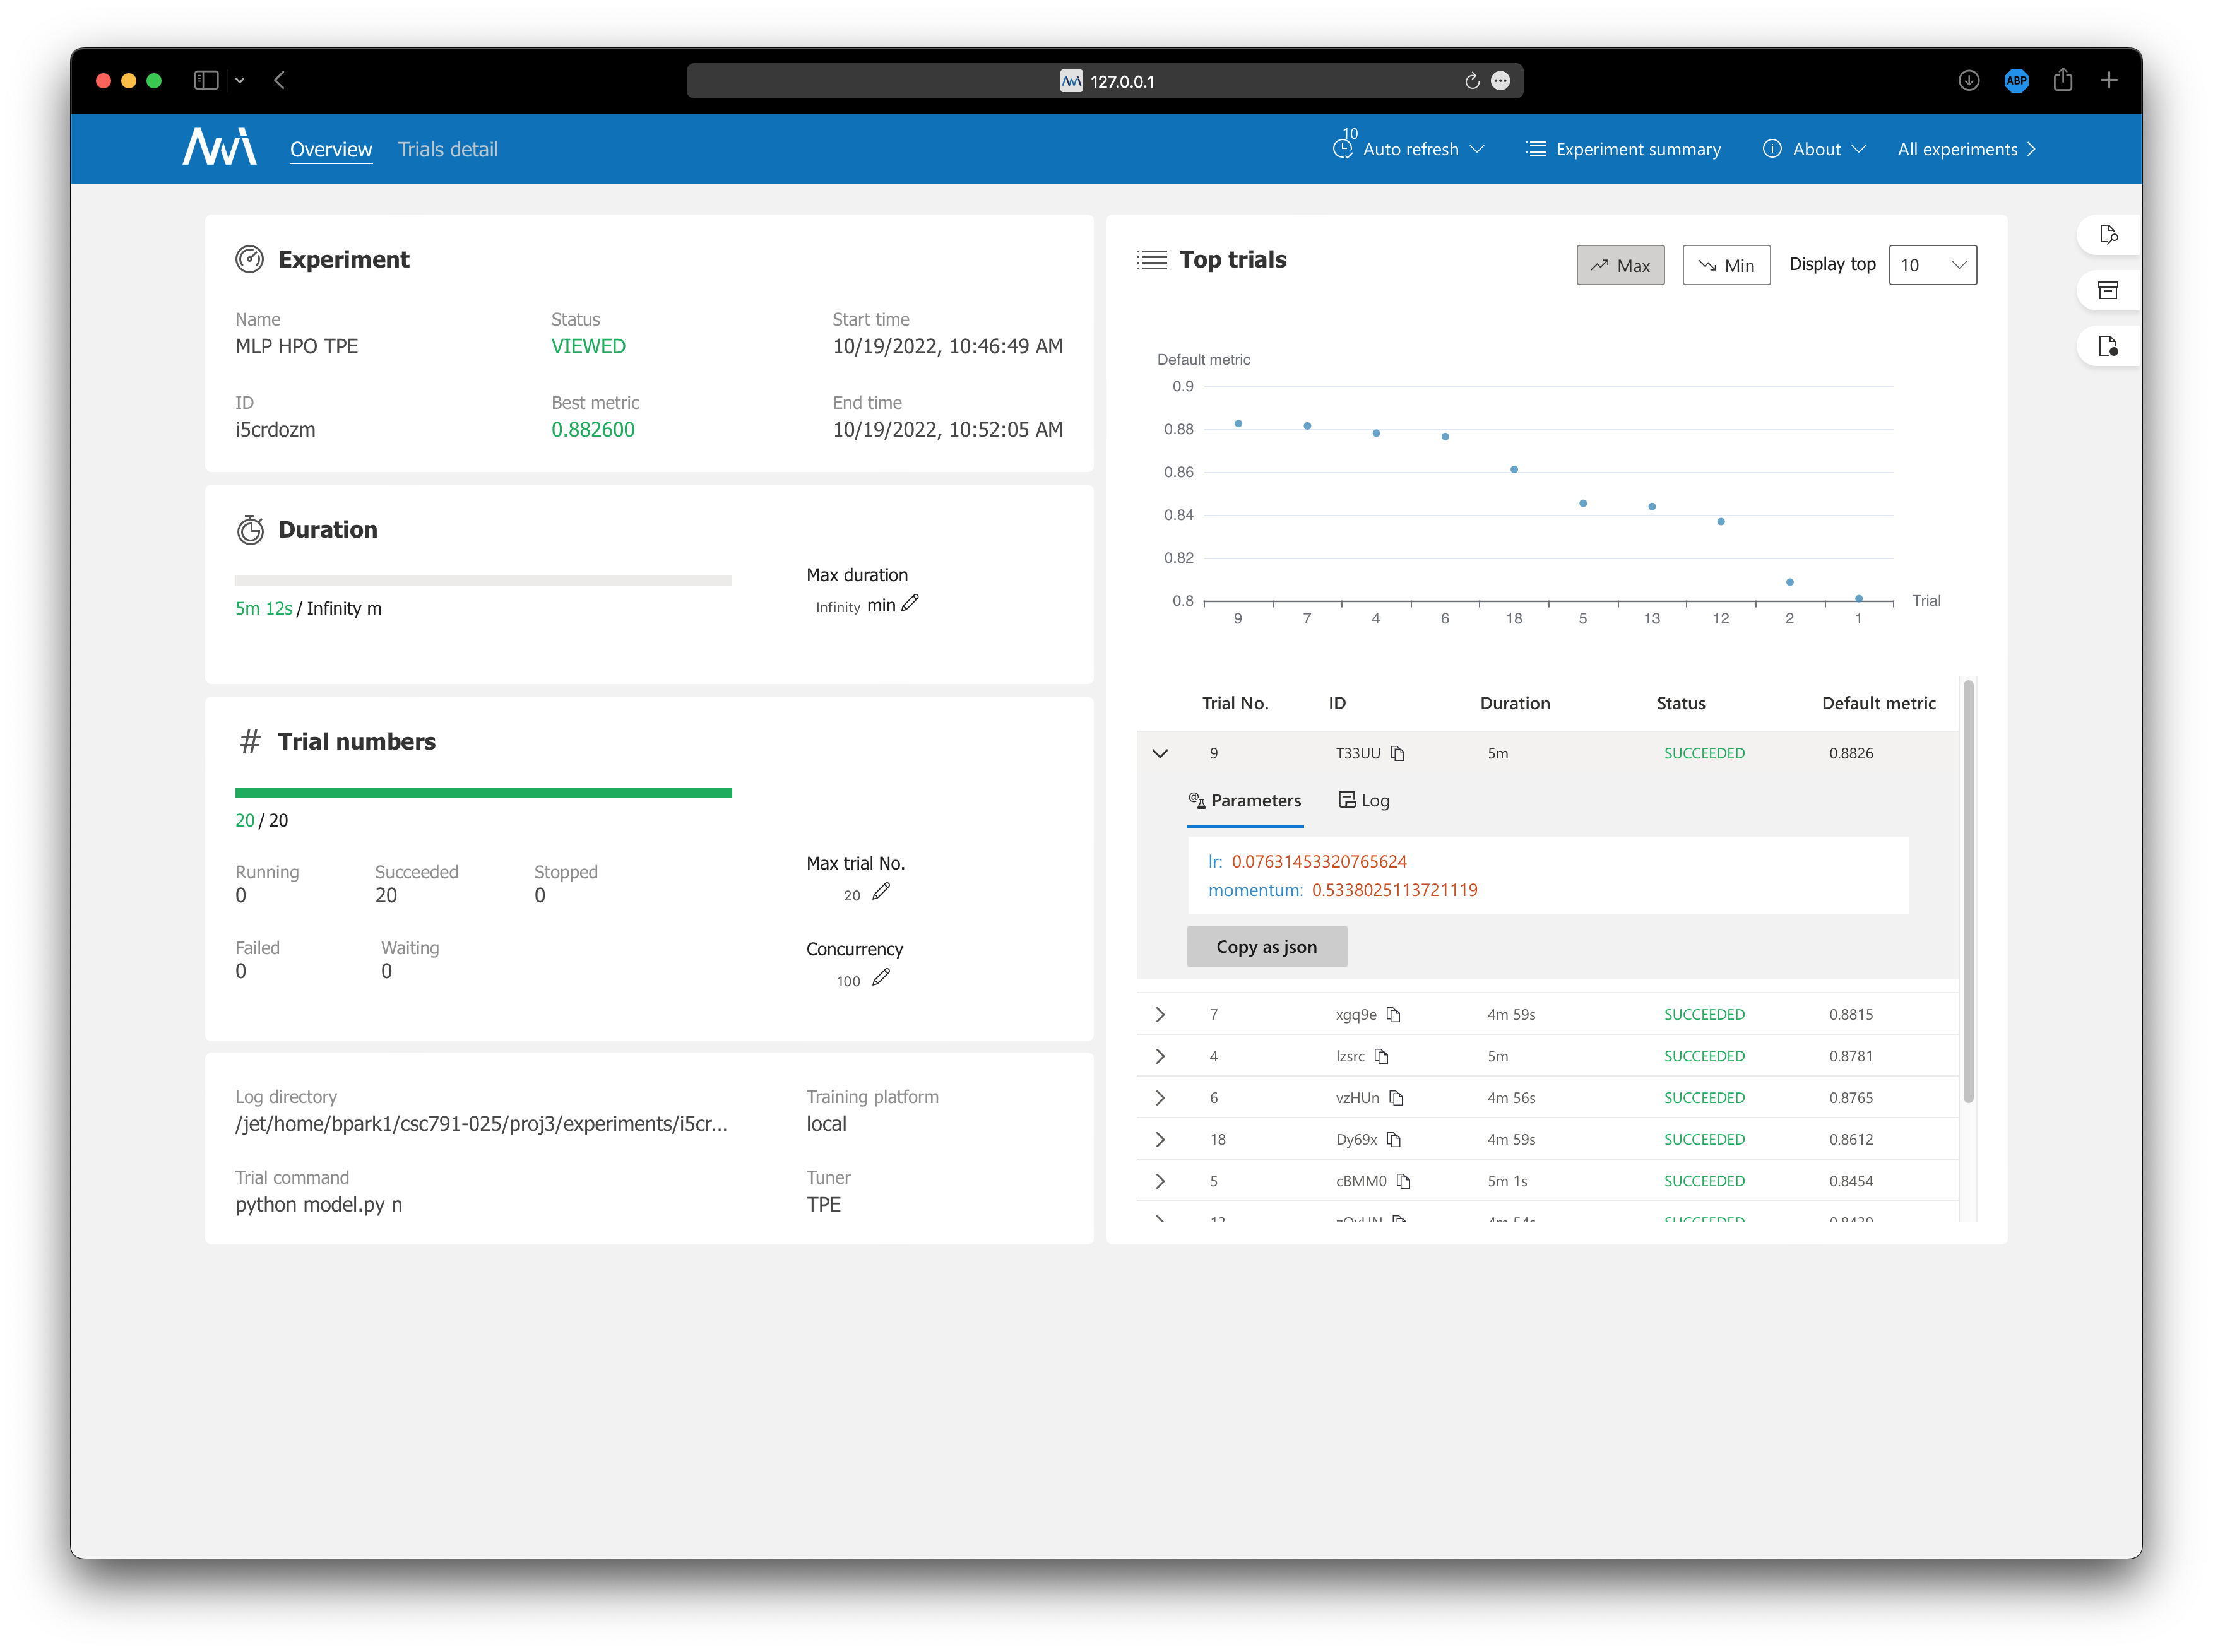
\includegraphics[width=3.5in]{../proj3/figures/mlp_tpe_overview.png}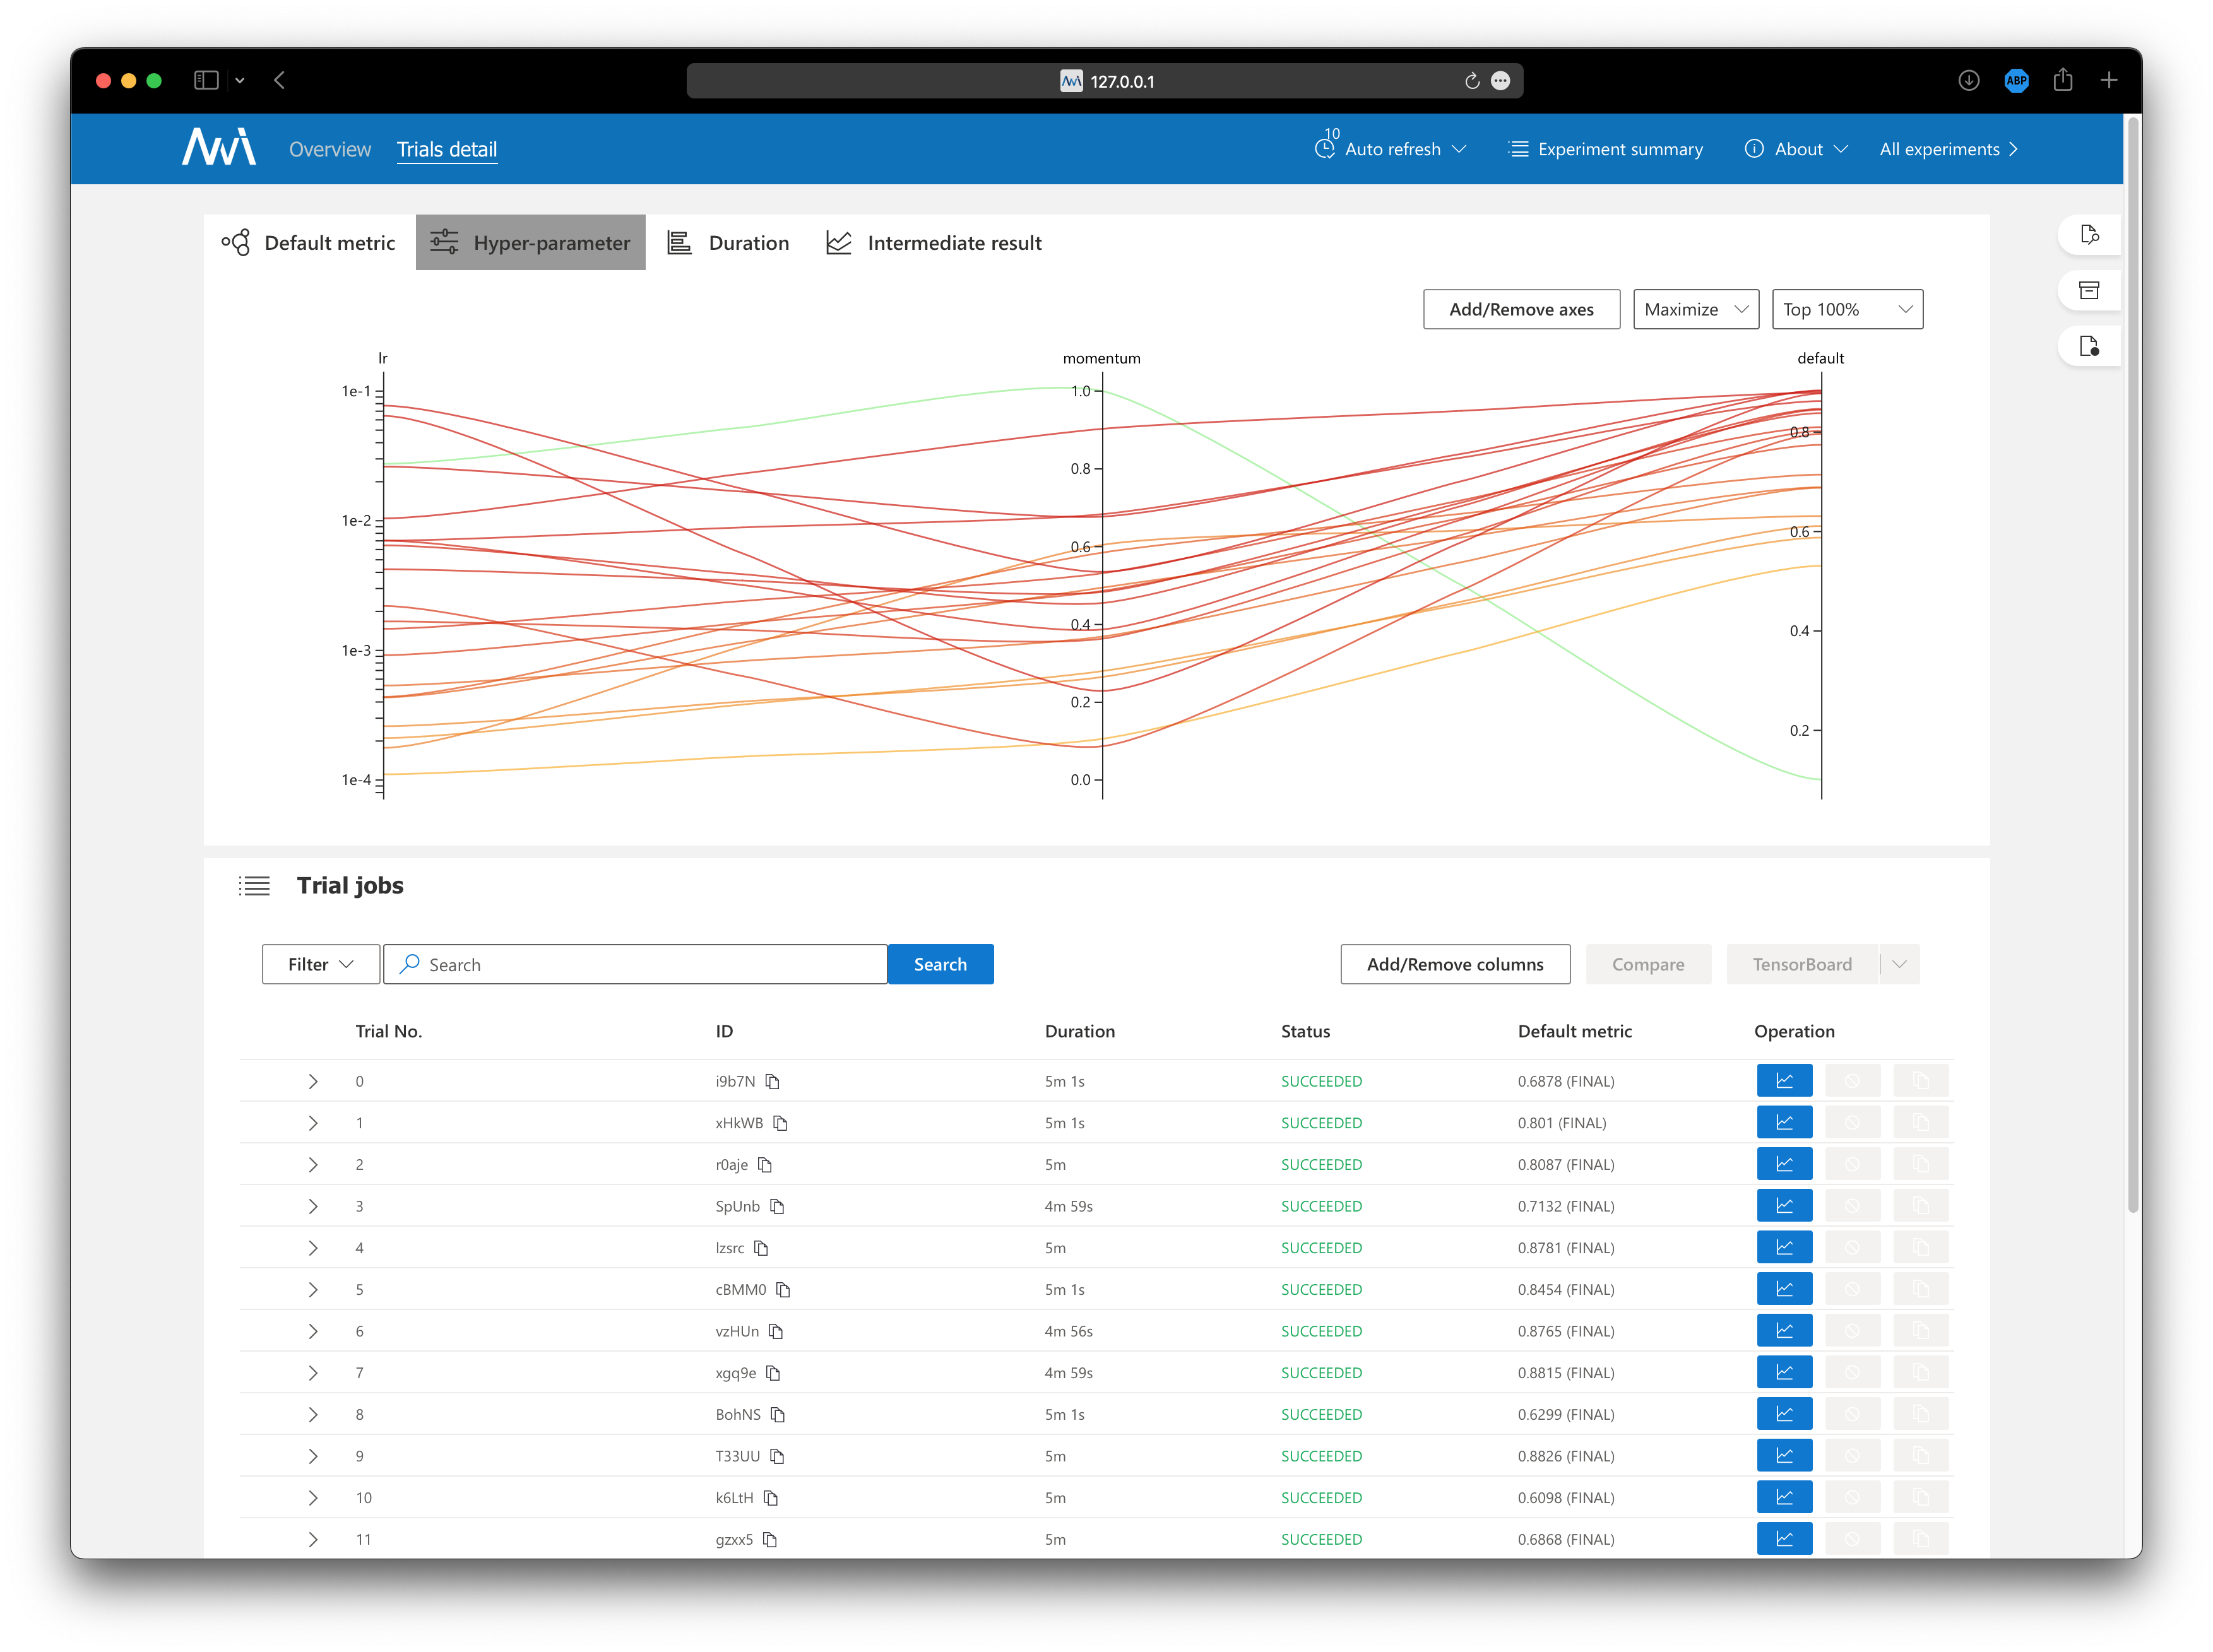
\includegraphics[width=3.5in]{../proj3/figures/mlp_tpe_hyperparameter.png}}
    \centerline{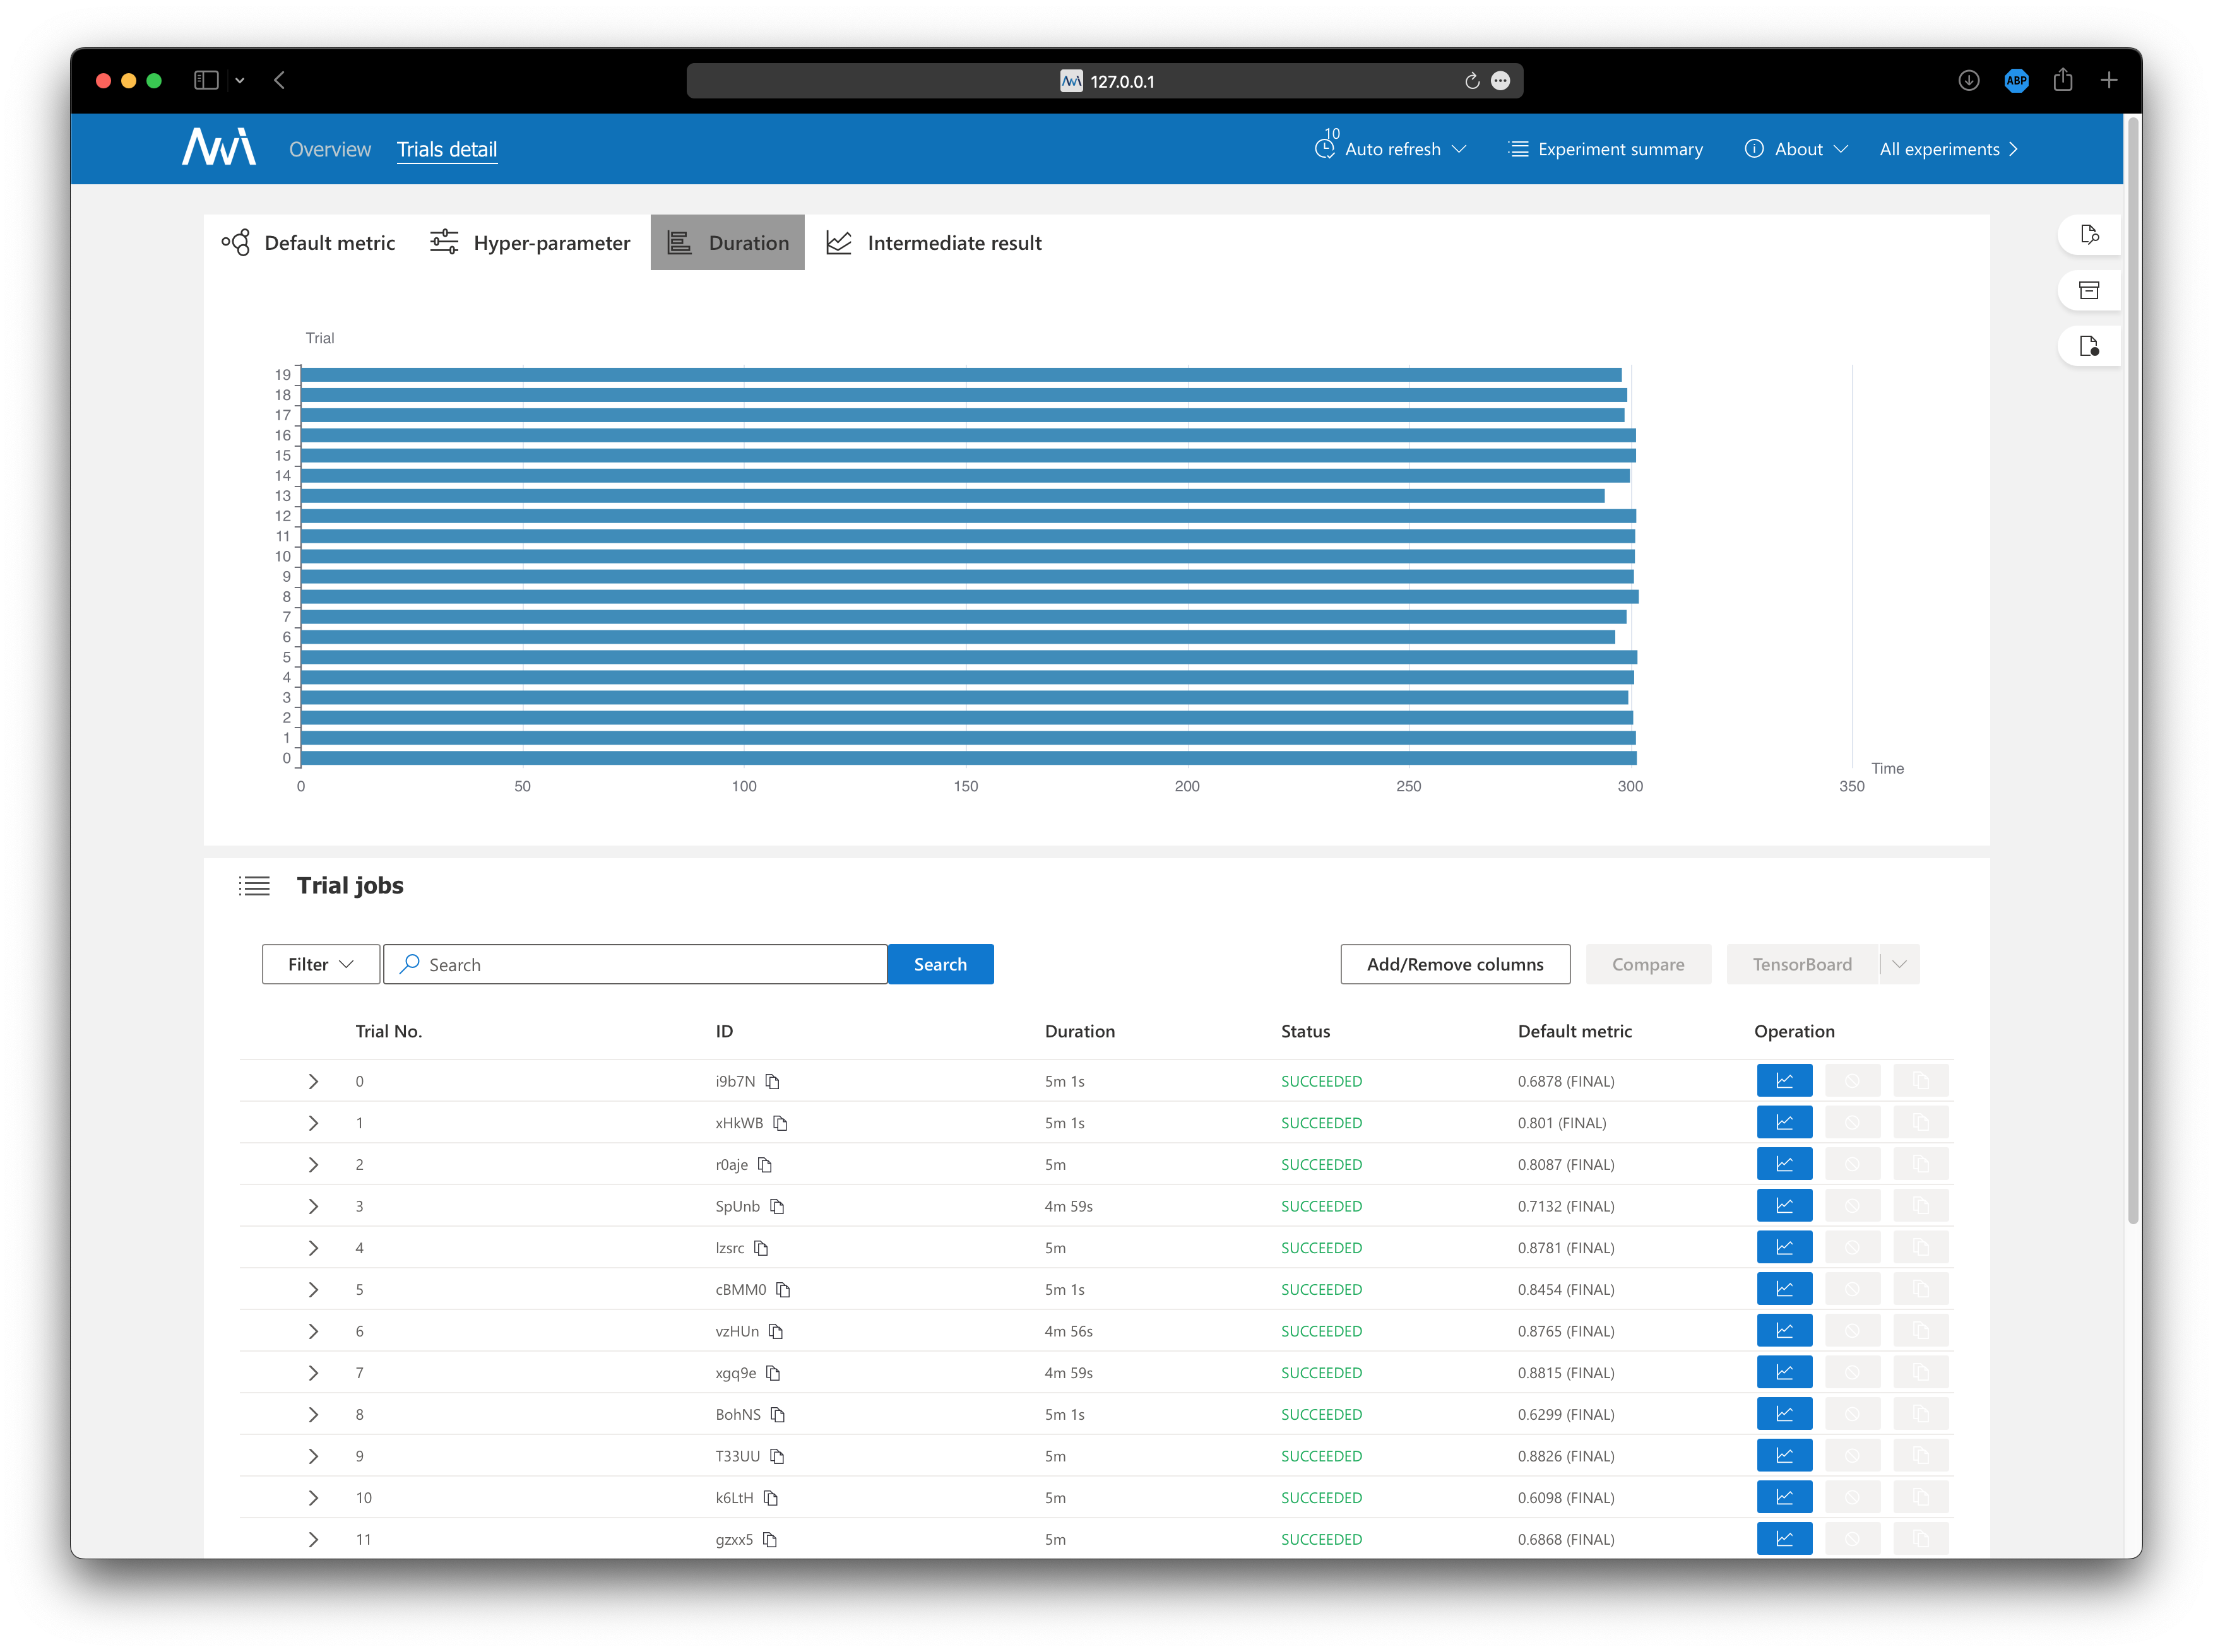
\includegraphics[width=3.5in]{../proj3/figures/mlp_tpe_latency.png}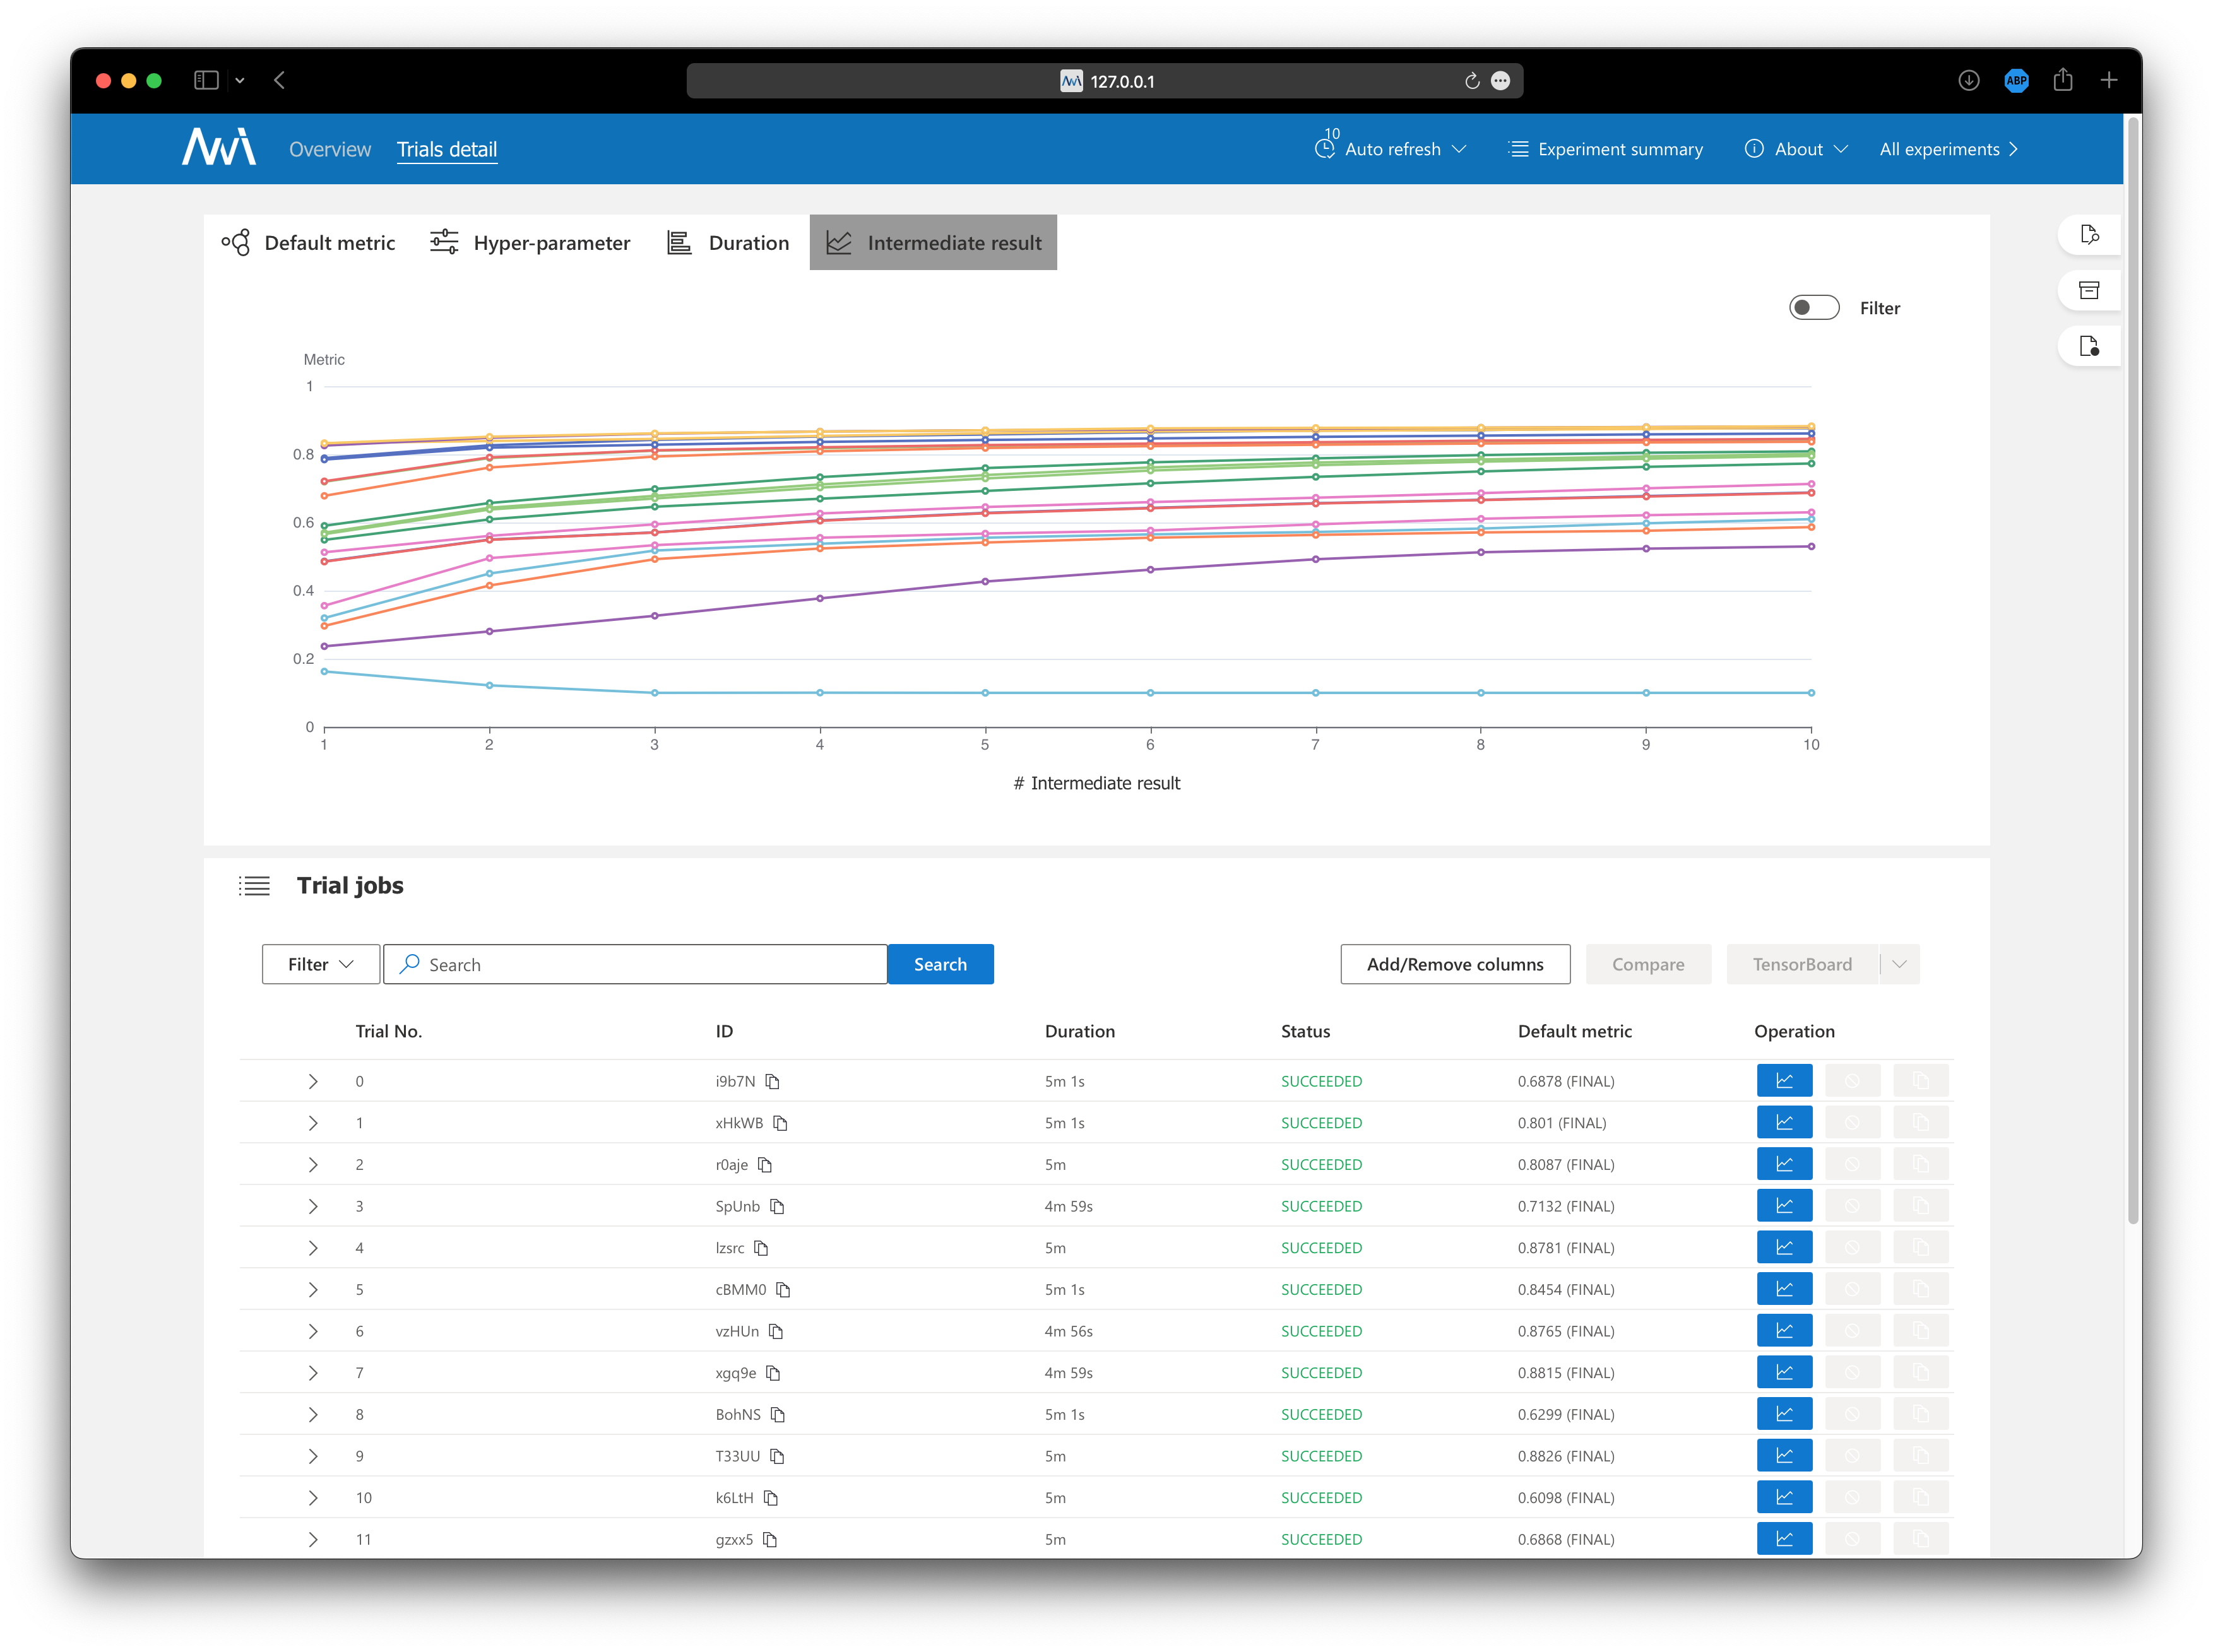
\includegraphics[width=3.5in]{../proj3/figures/mlp_tpe_intermediate.png}}
    \caption{MLP with TPE Tuner on Learning Rate and Momentum}
    \label{fig:mlp-tpe}
\end{figure}

\begin{figure}
    \centerline{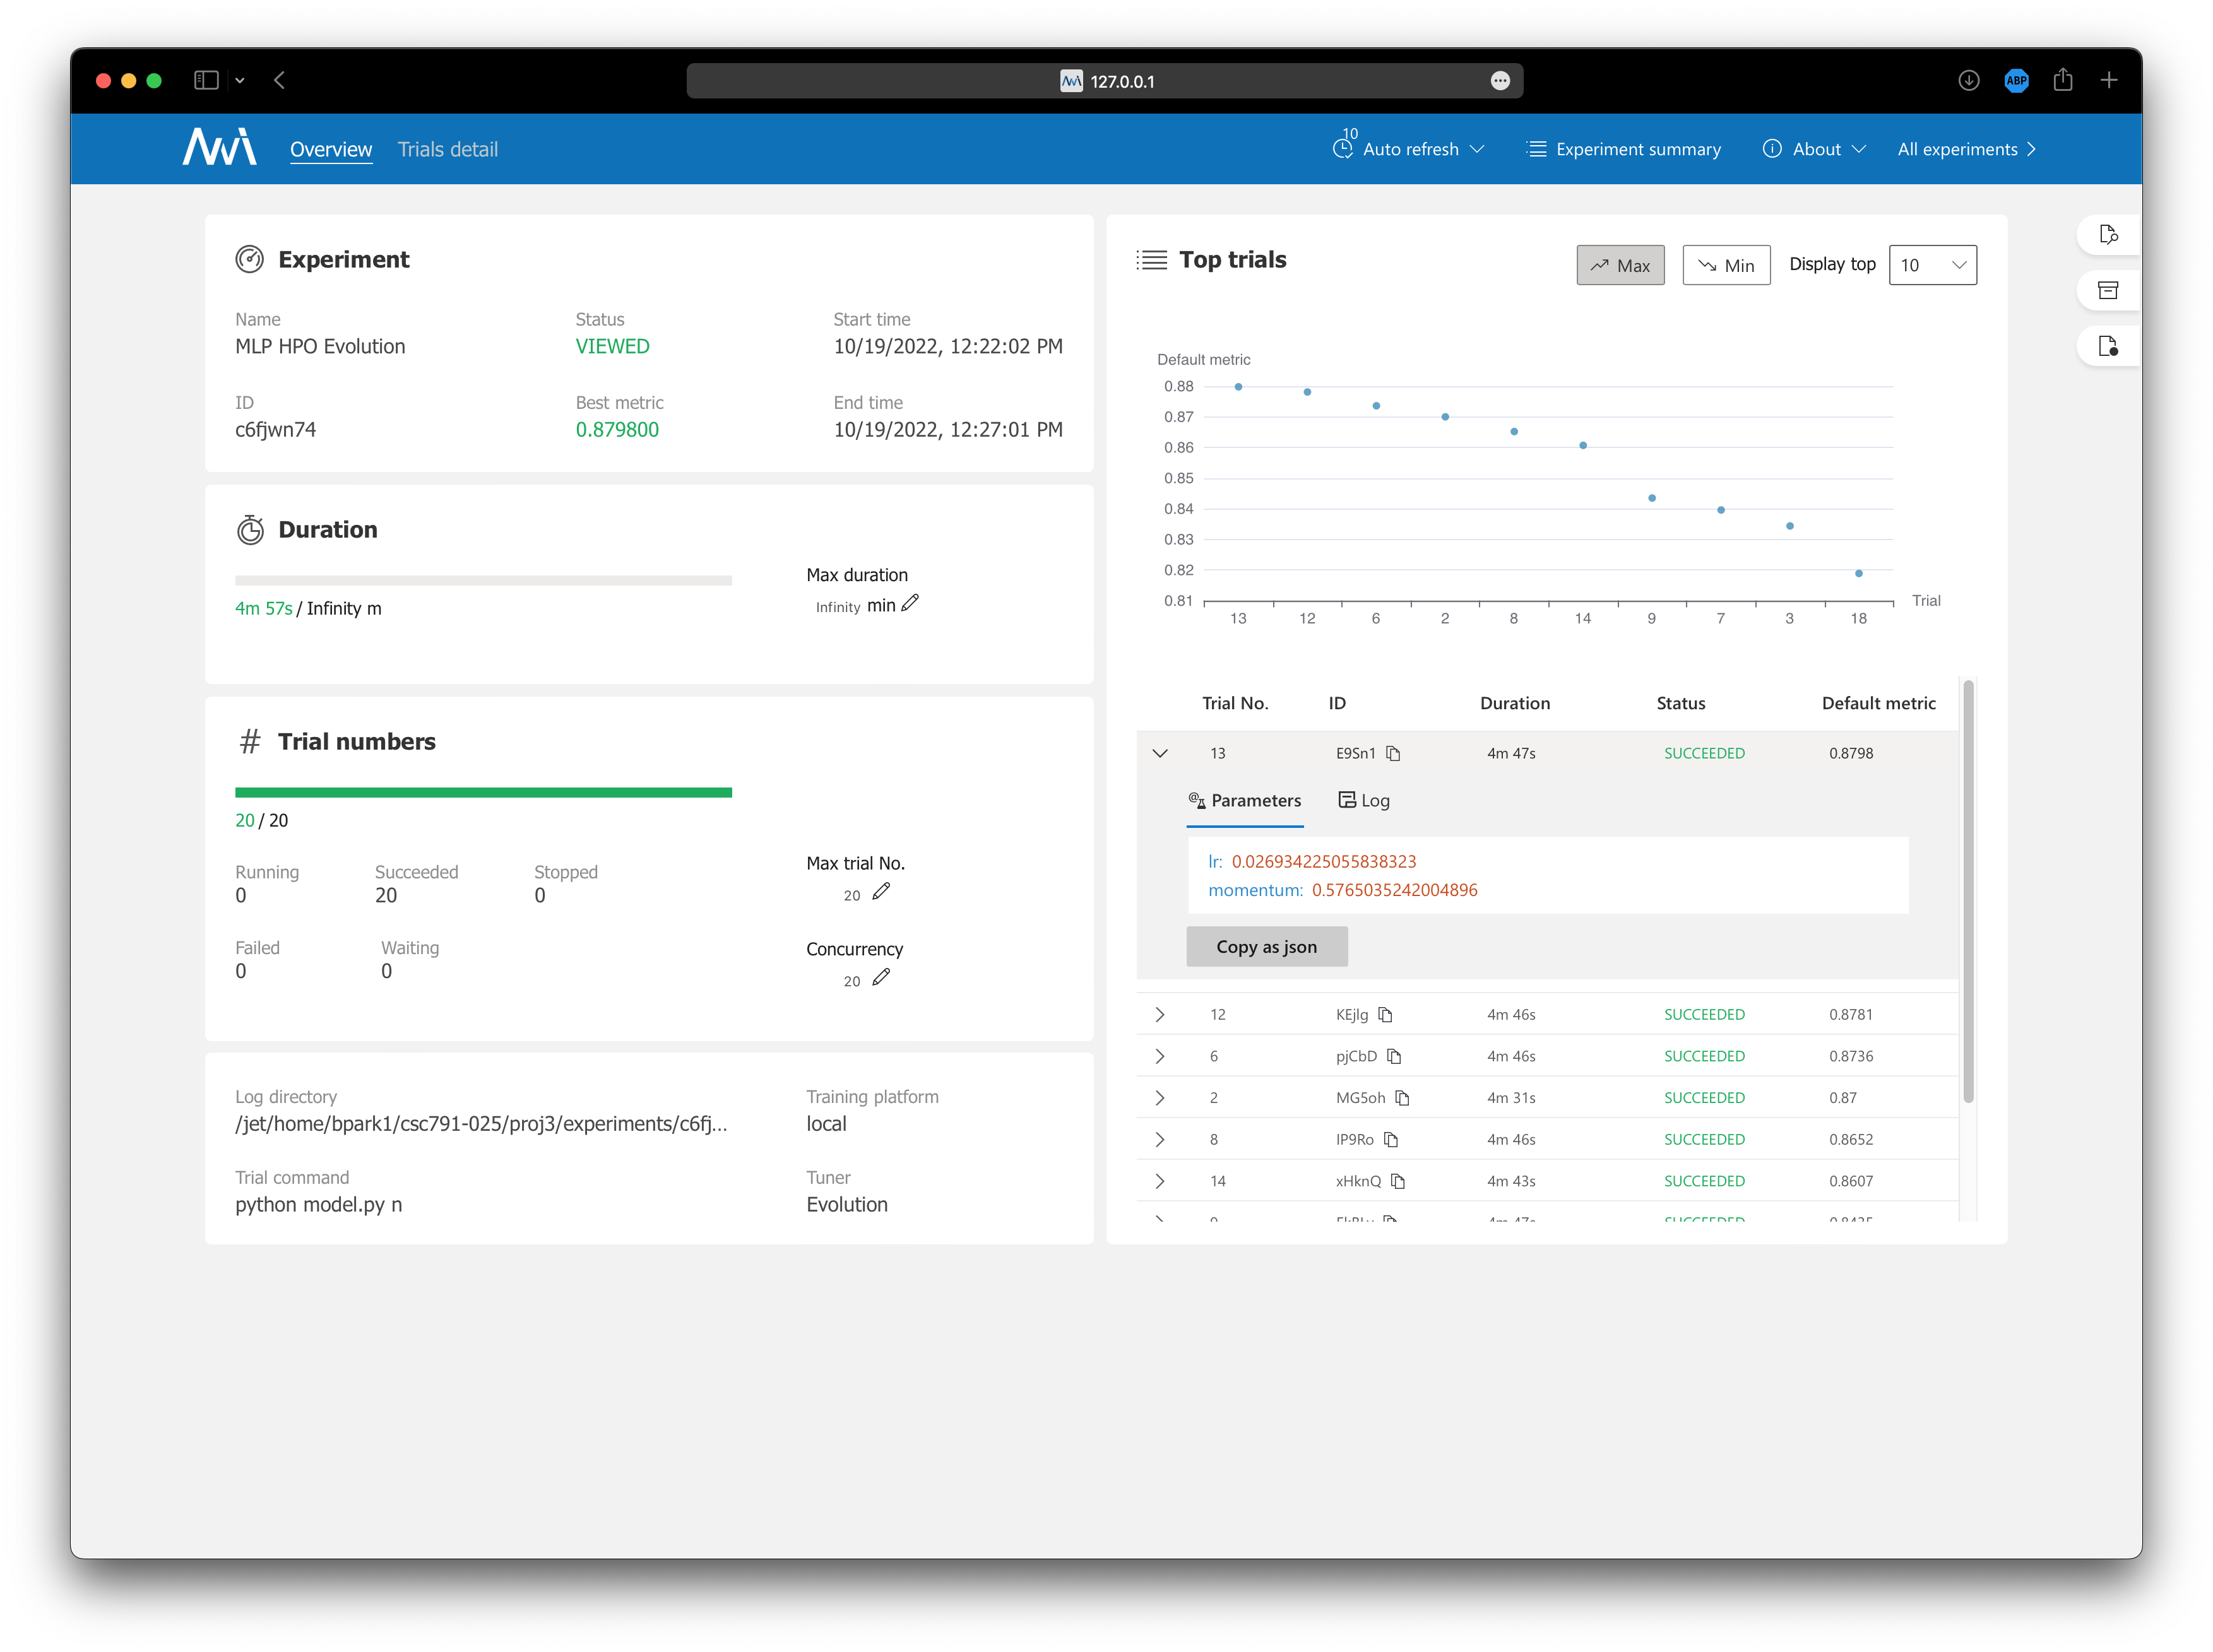
\includegraphics[width=3.5in]{../proj3/figures/mlp_evolution_overview.png}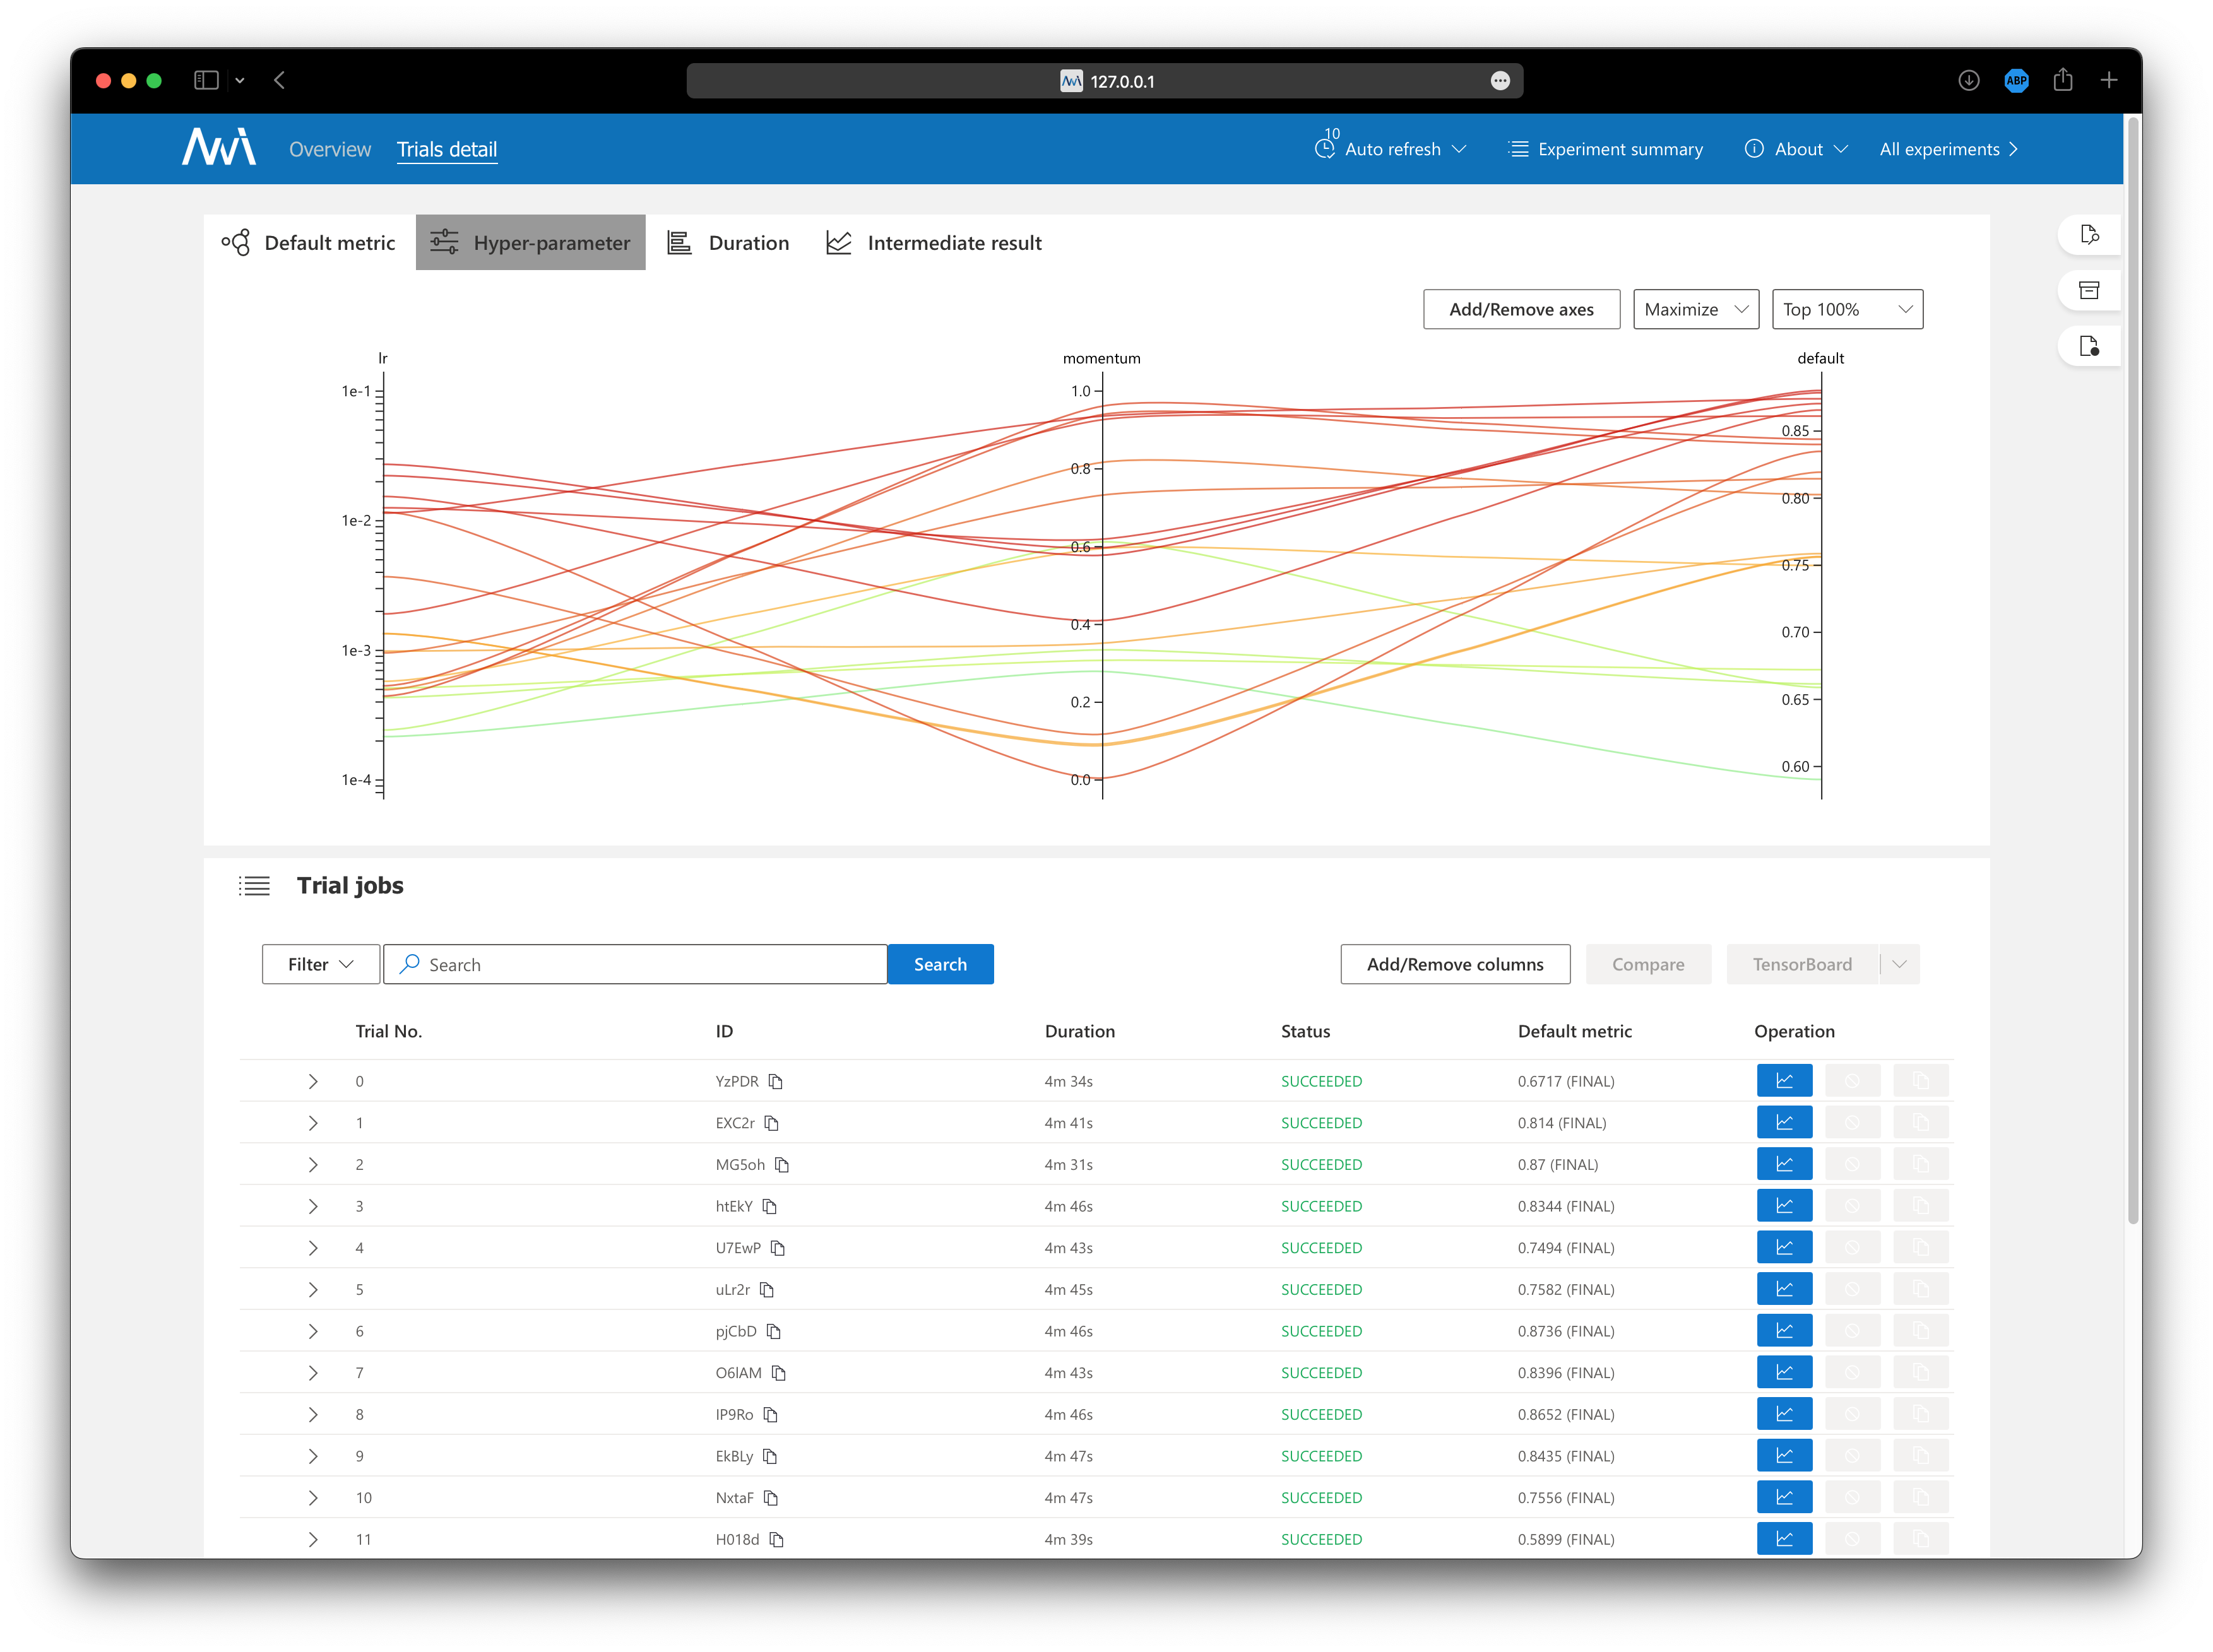
\includegraphics[width=3.5in]{../proj3/figures/mlp_evolution_hyperparameter.png}}
    \centerline{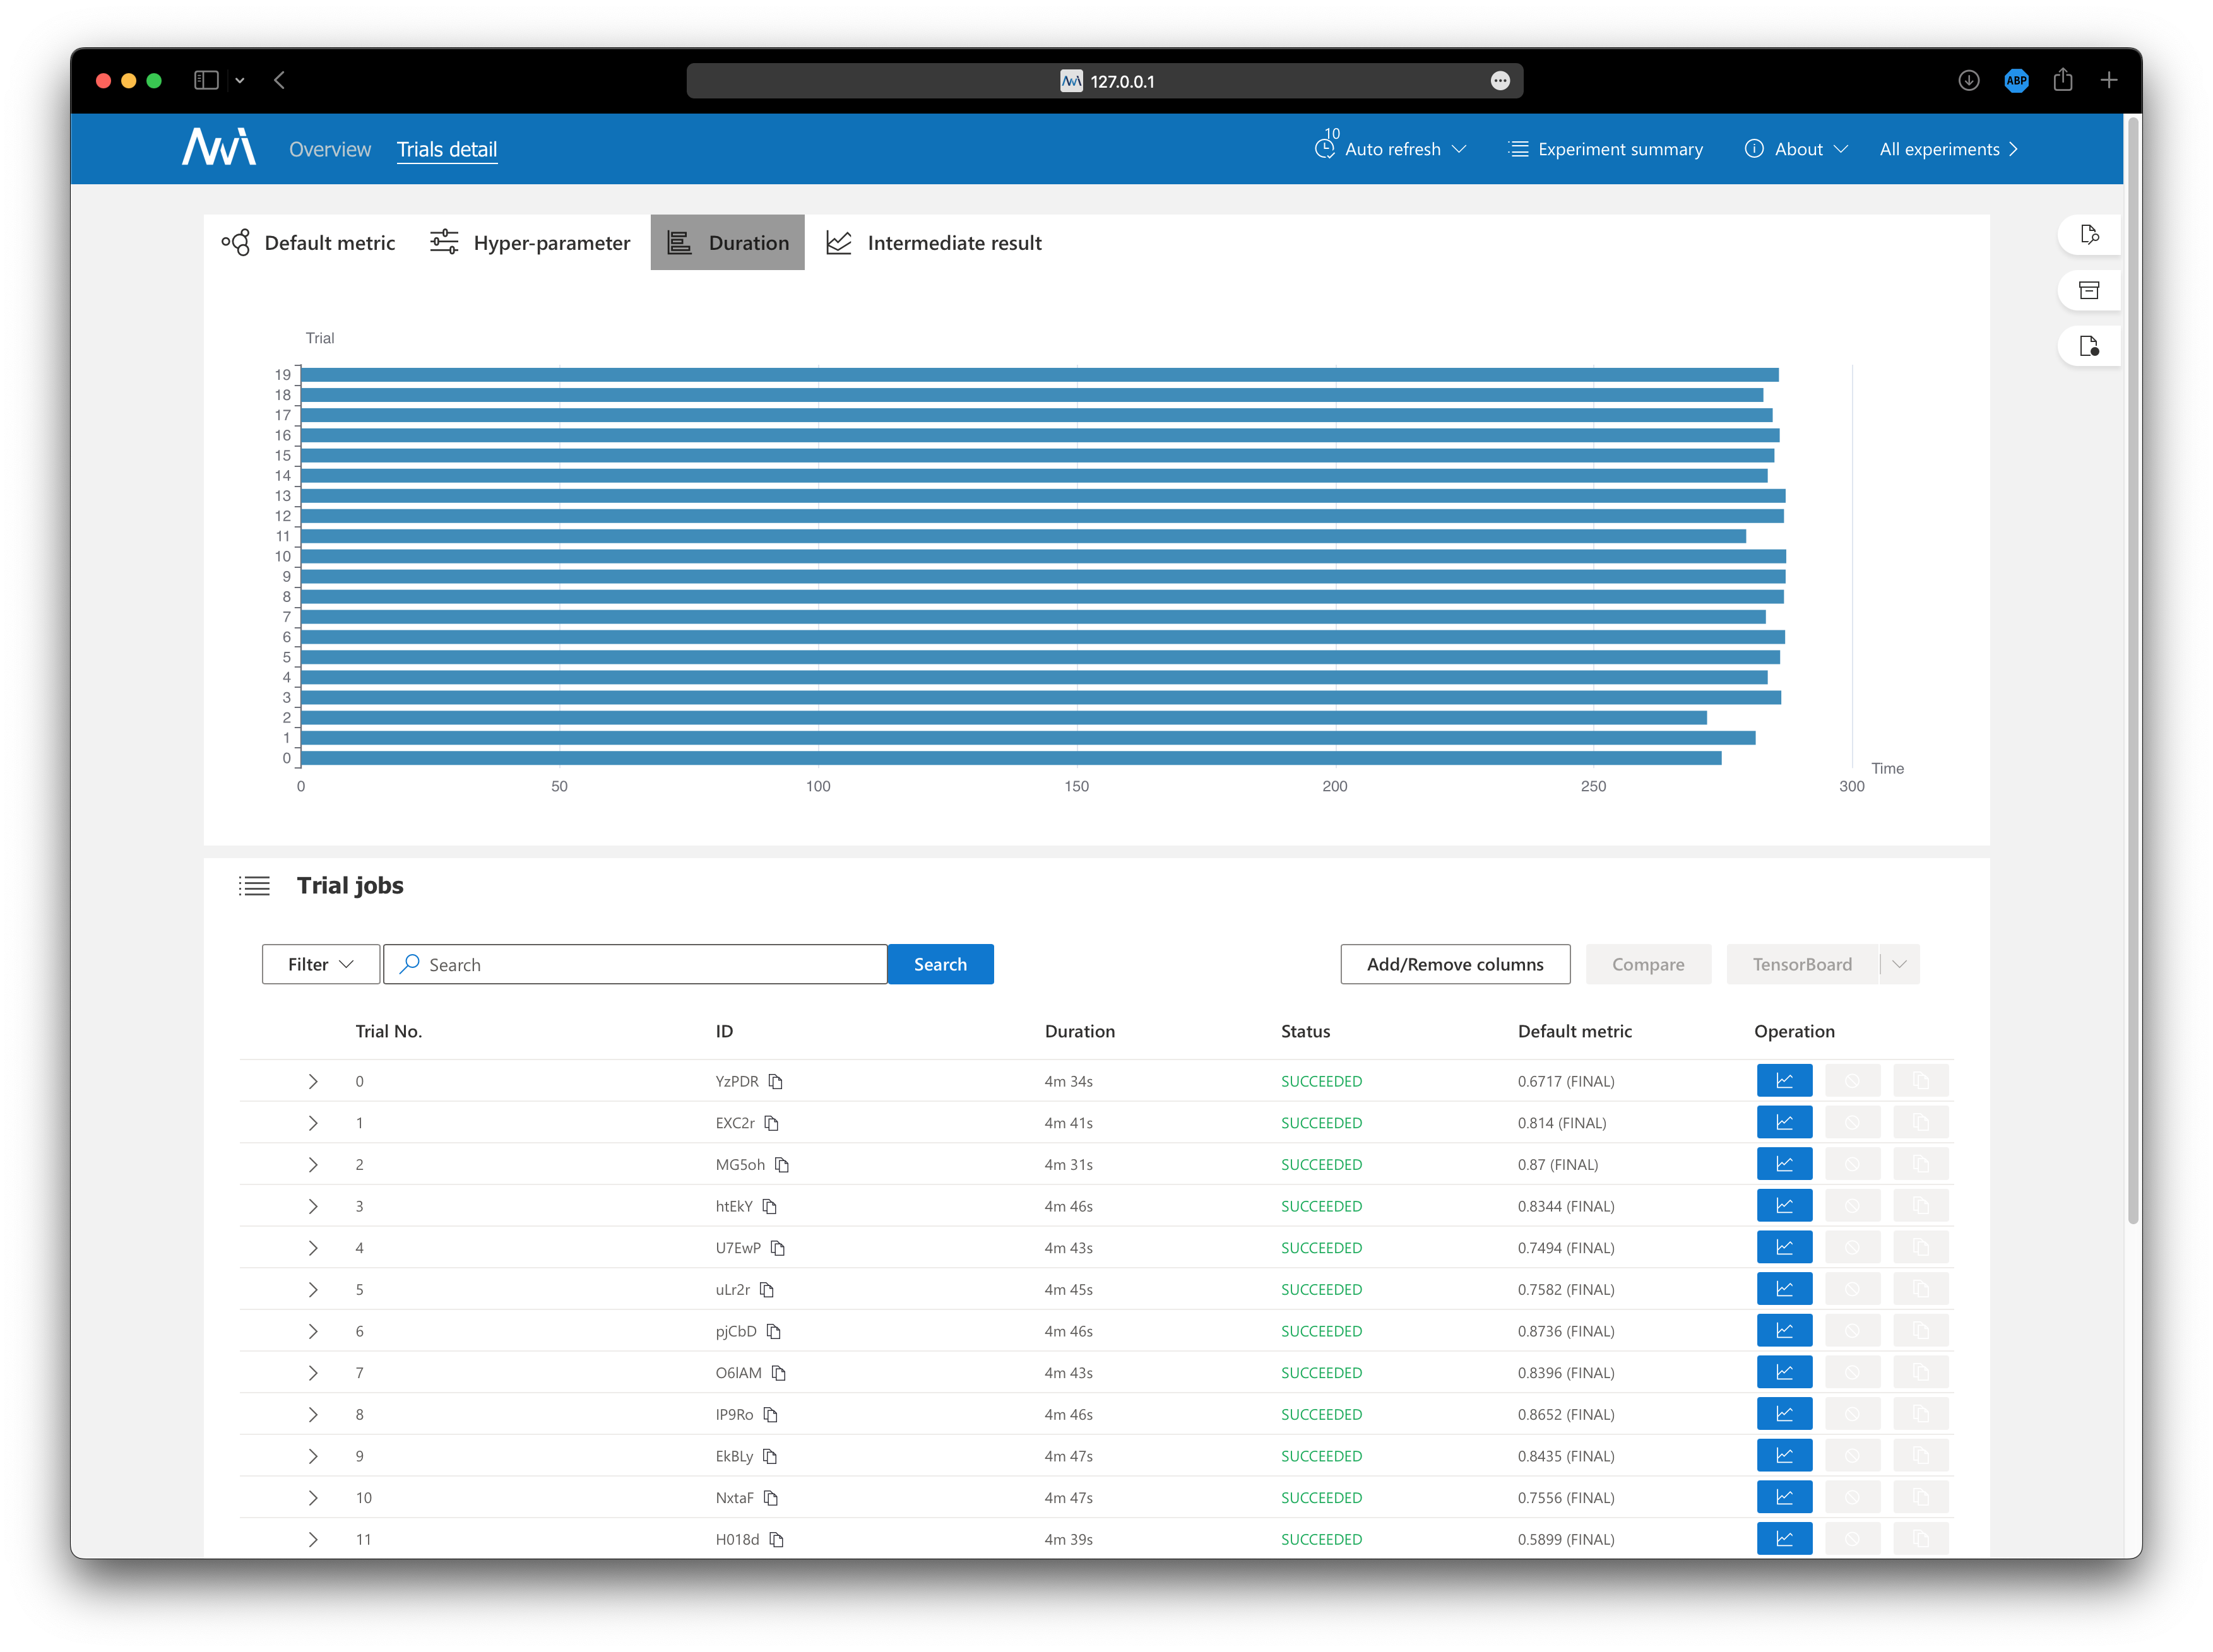
\includegraphics[width=3.5in]{../proj3/figures/mlp_evolution_latency.png}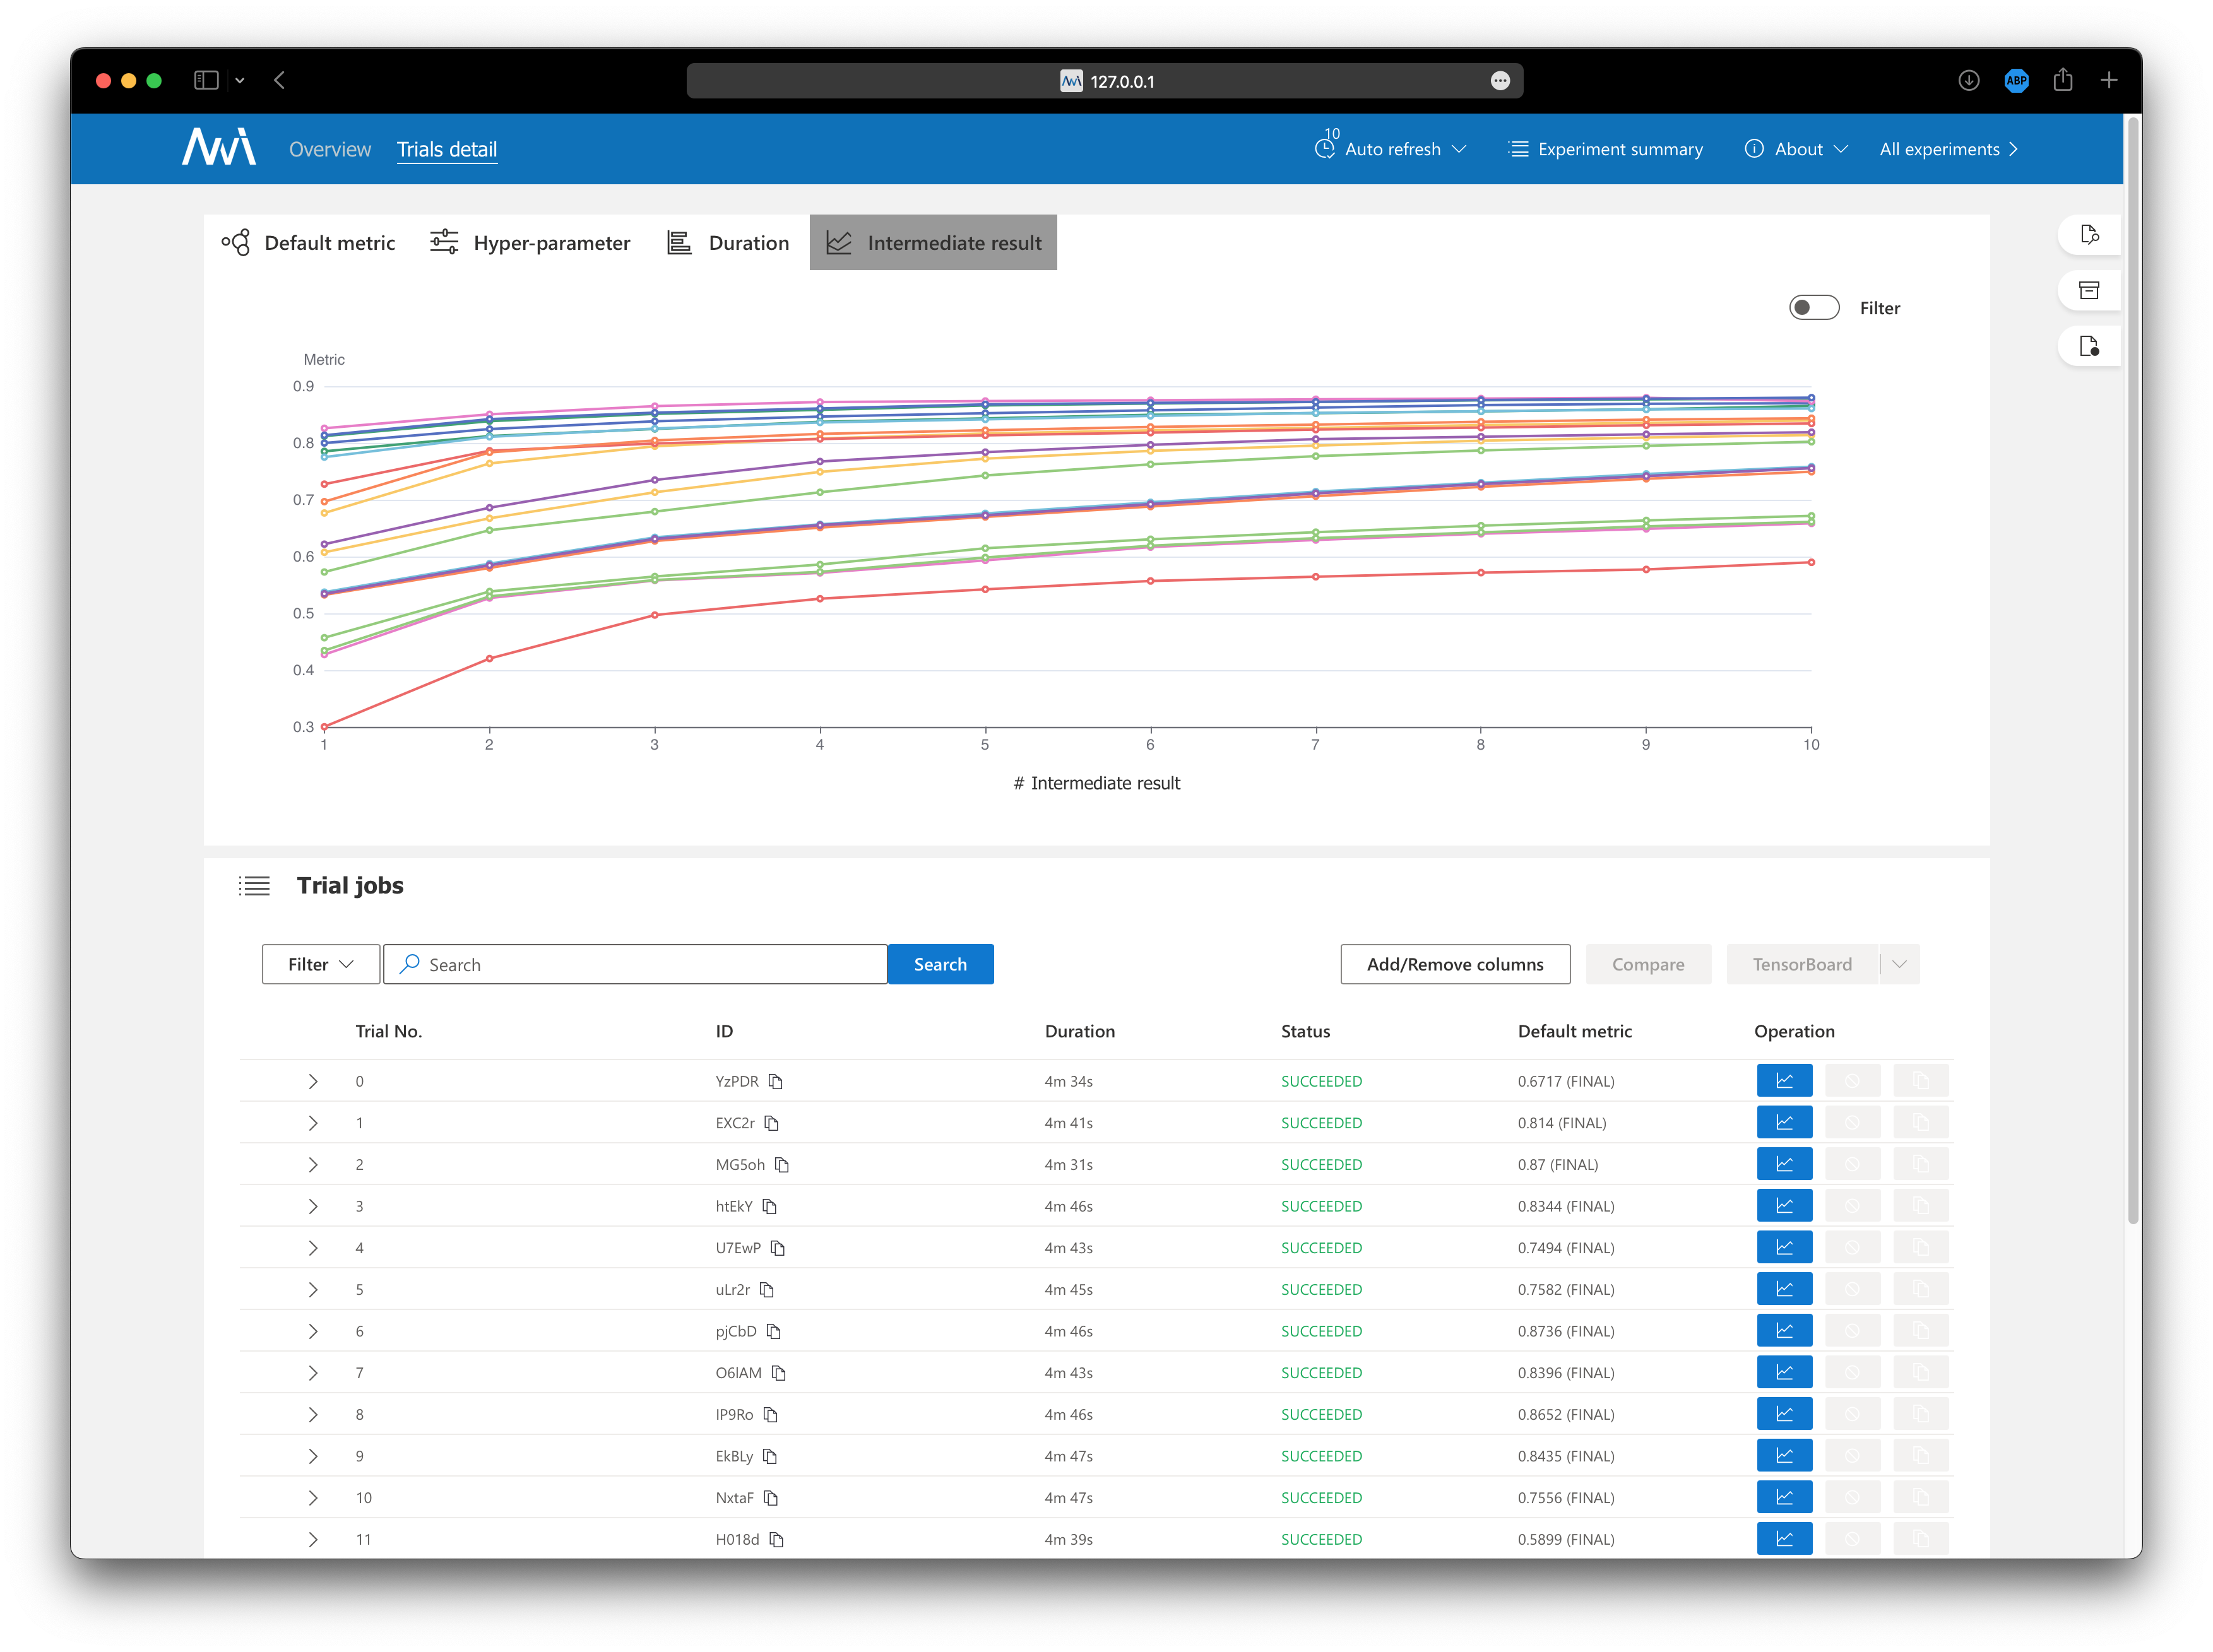
\includegraphics[width=3.5in]{../proj3/figures/mlp_evolution_intermediate.png}}
    \caption{MLP with Evolution Tuner on Learning Rate and Momentum}
    \label{fig:mlp-evolution}
\end{figure}

\begin{figure}
    \centerline{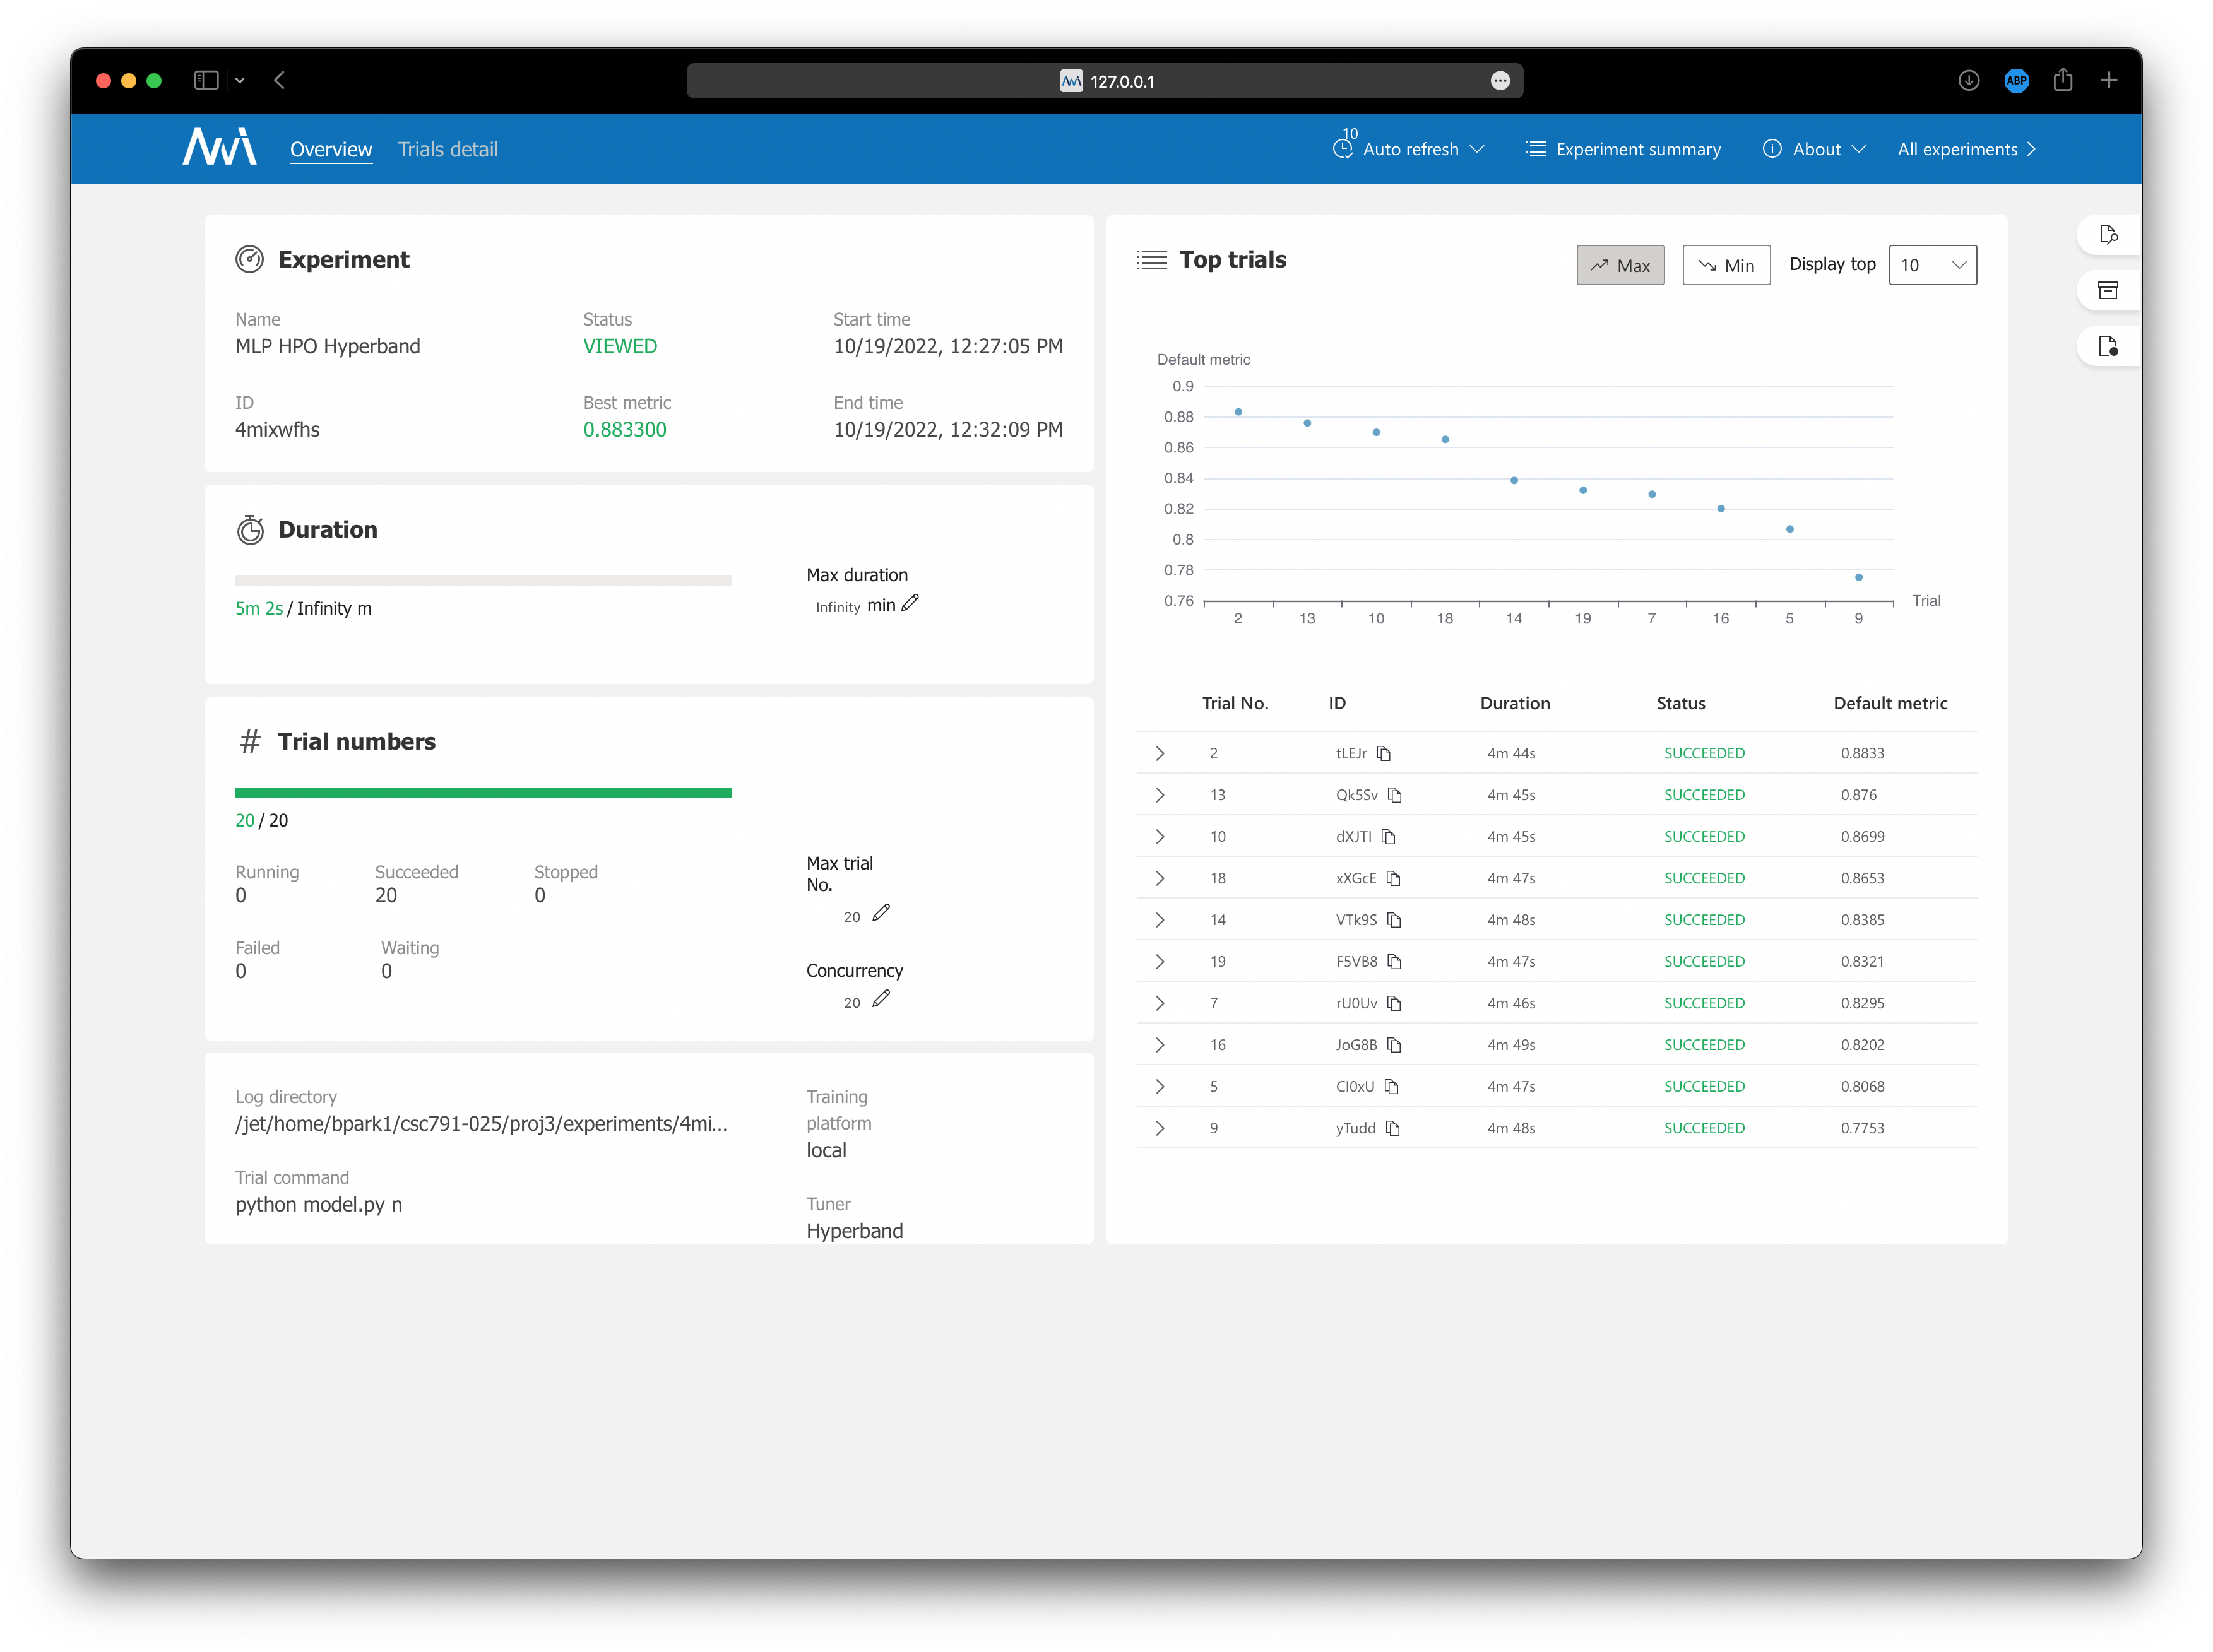
\includegraphics[width=3.5in]{../proj3/figures/mlp_hyperband_overview.png}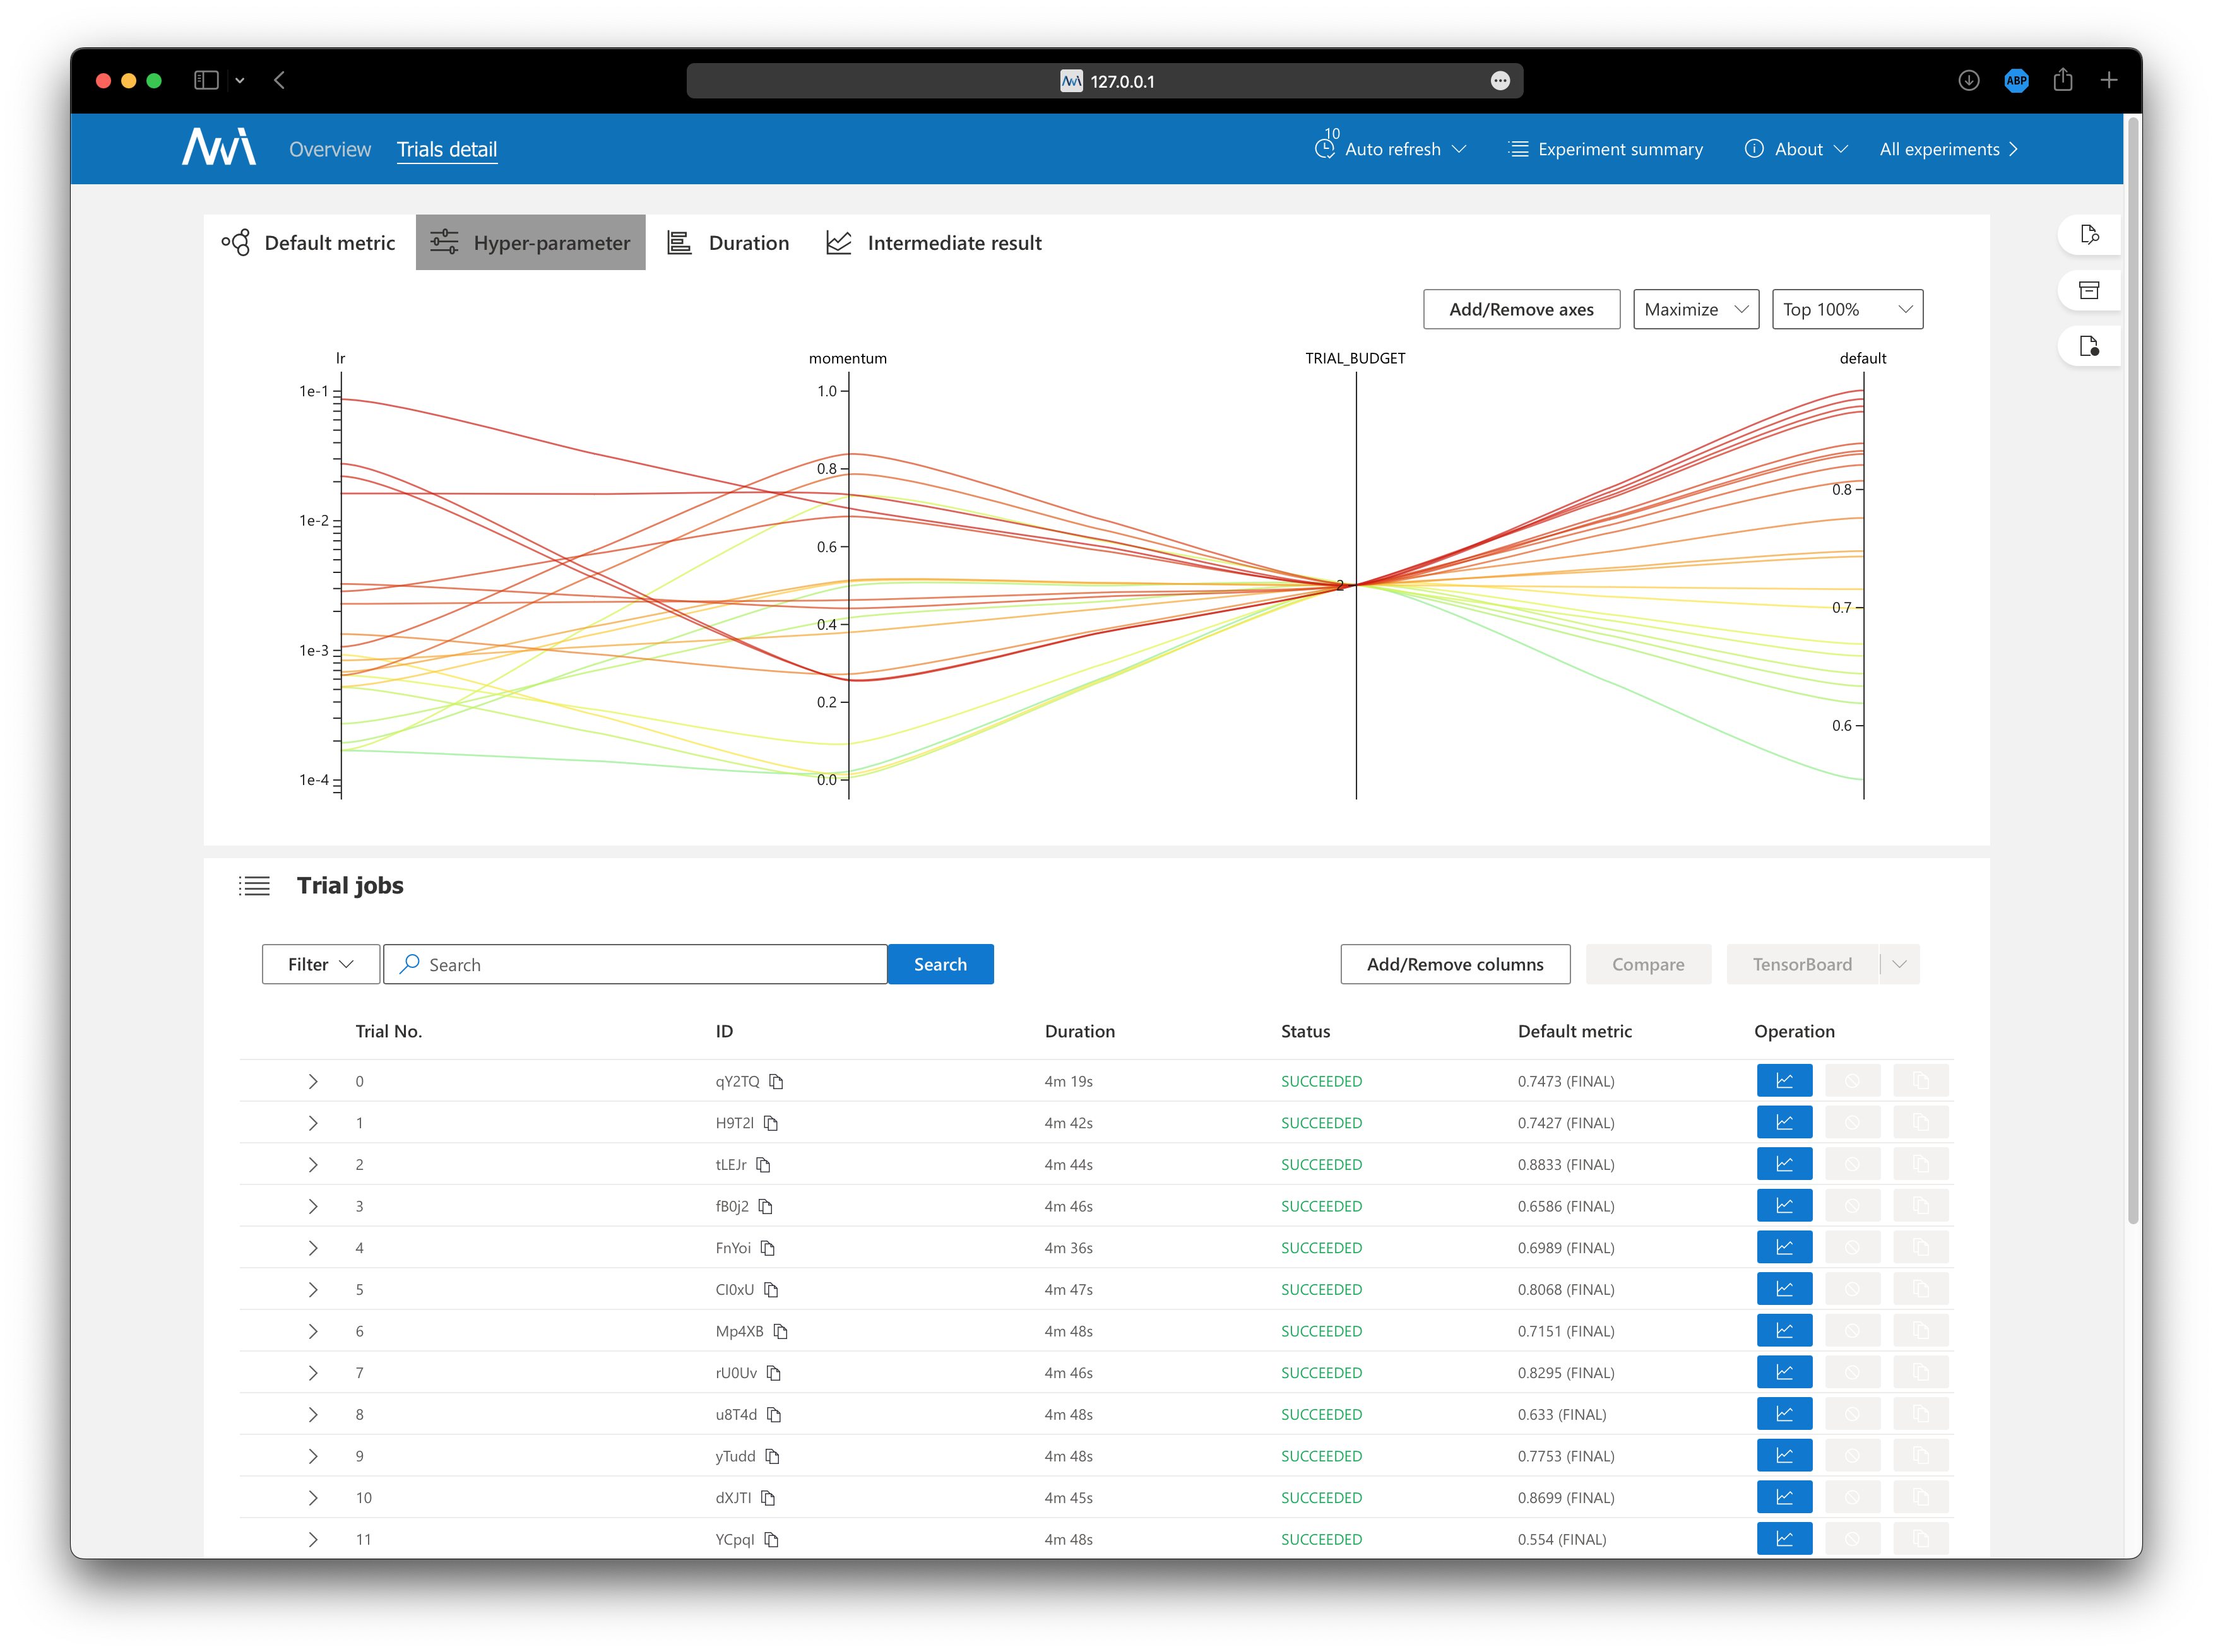
\includegraphics[width=3.5in]{../proj3/figures/mlp_hyperband_hyperparameter.png}}
    \centerline{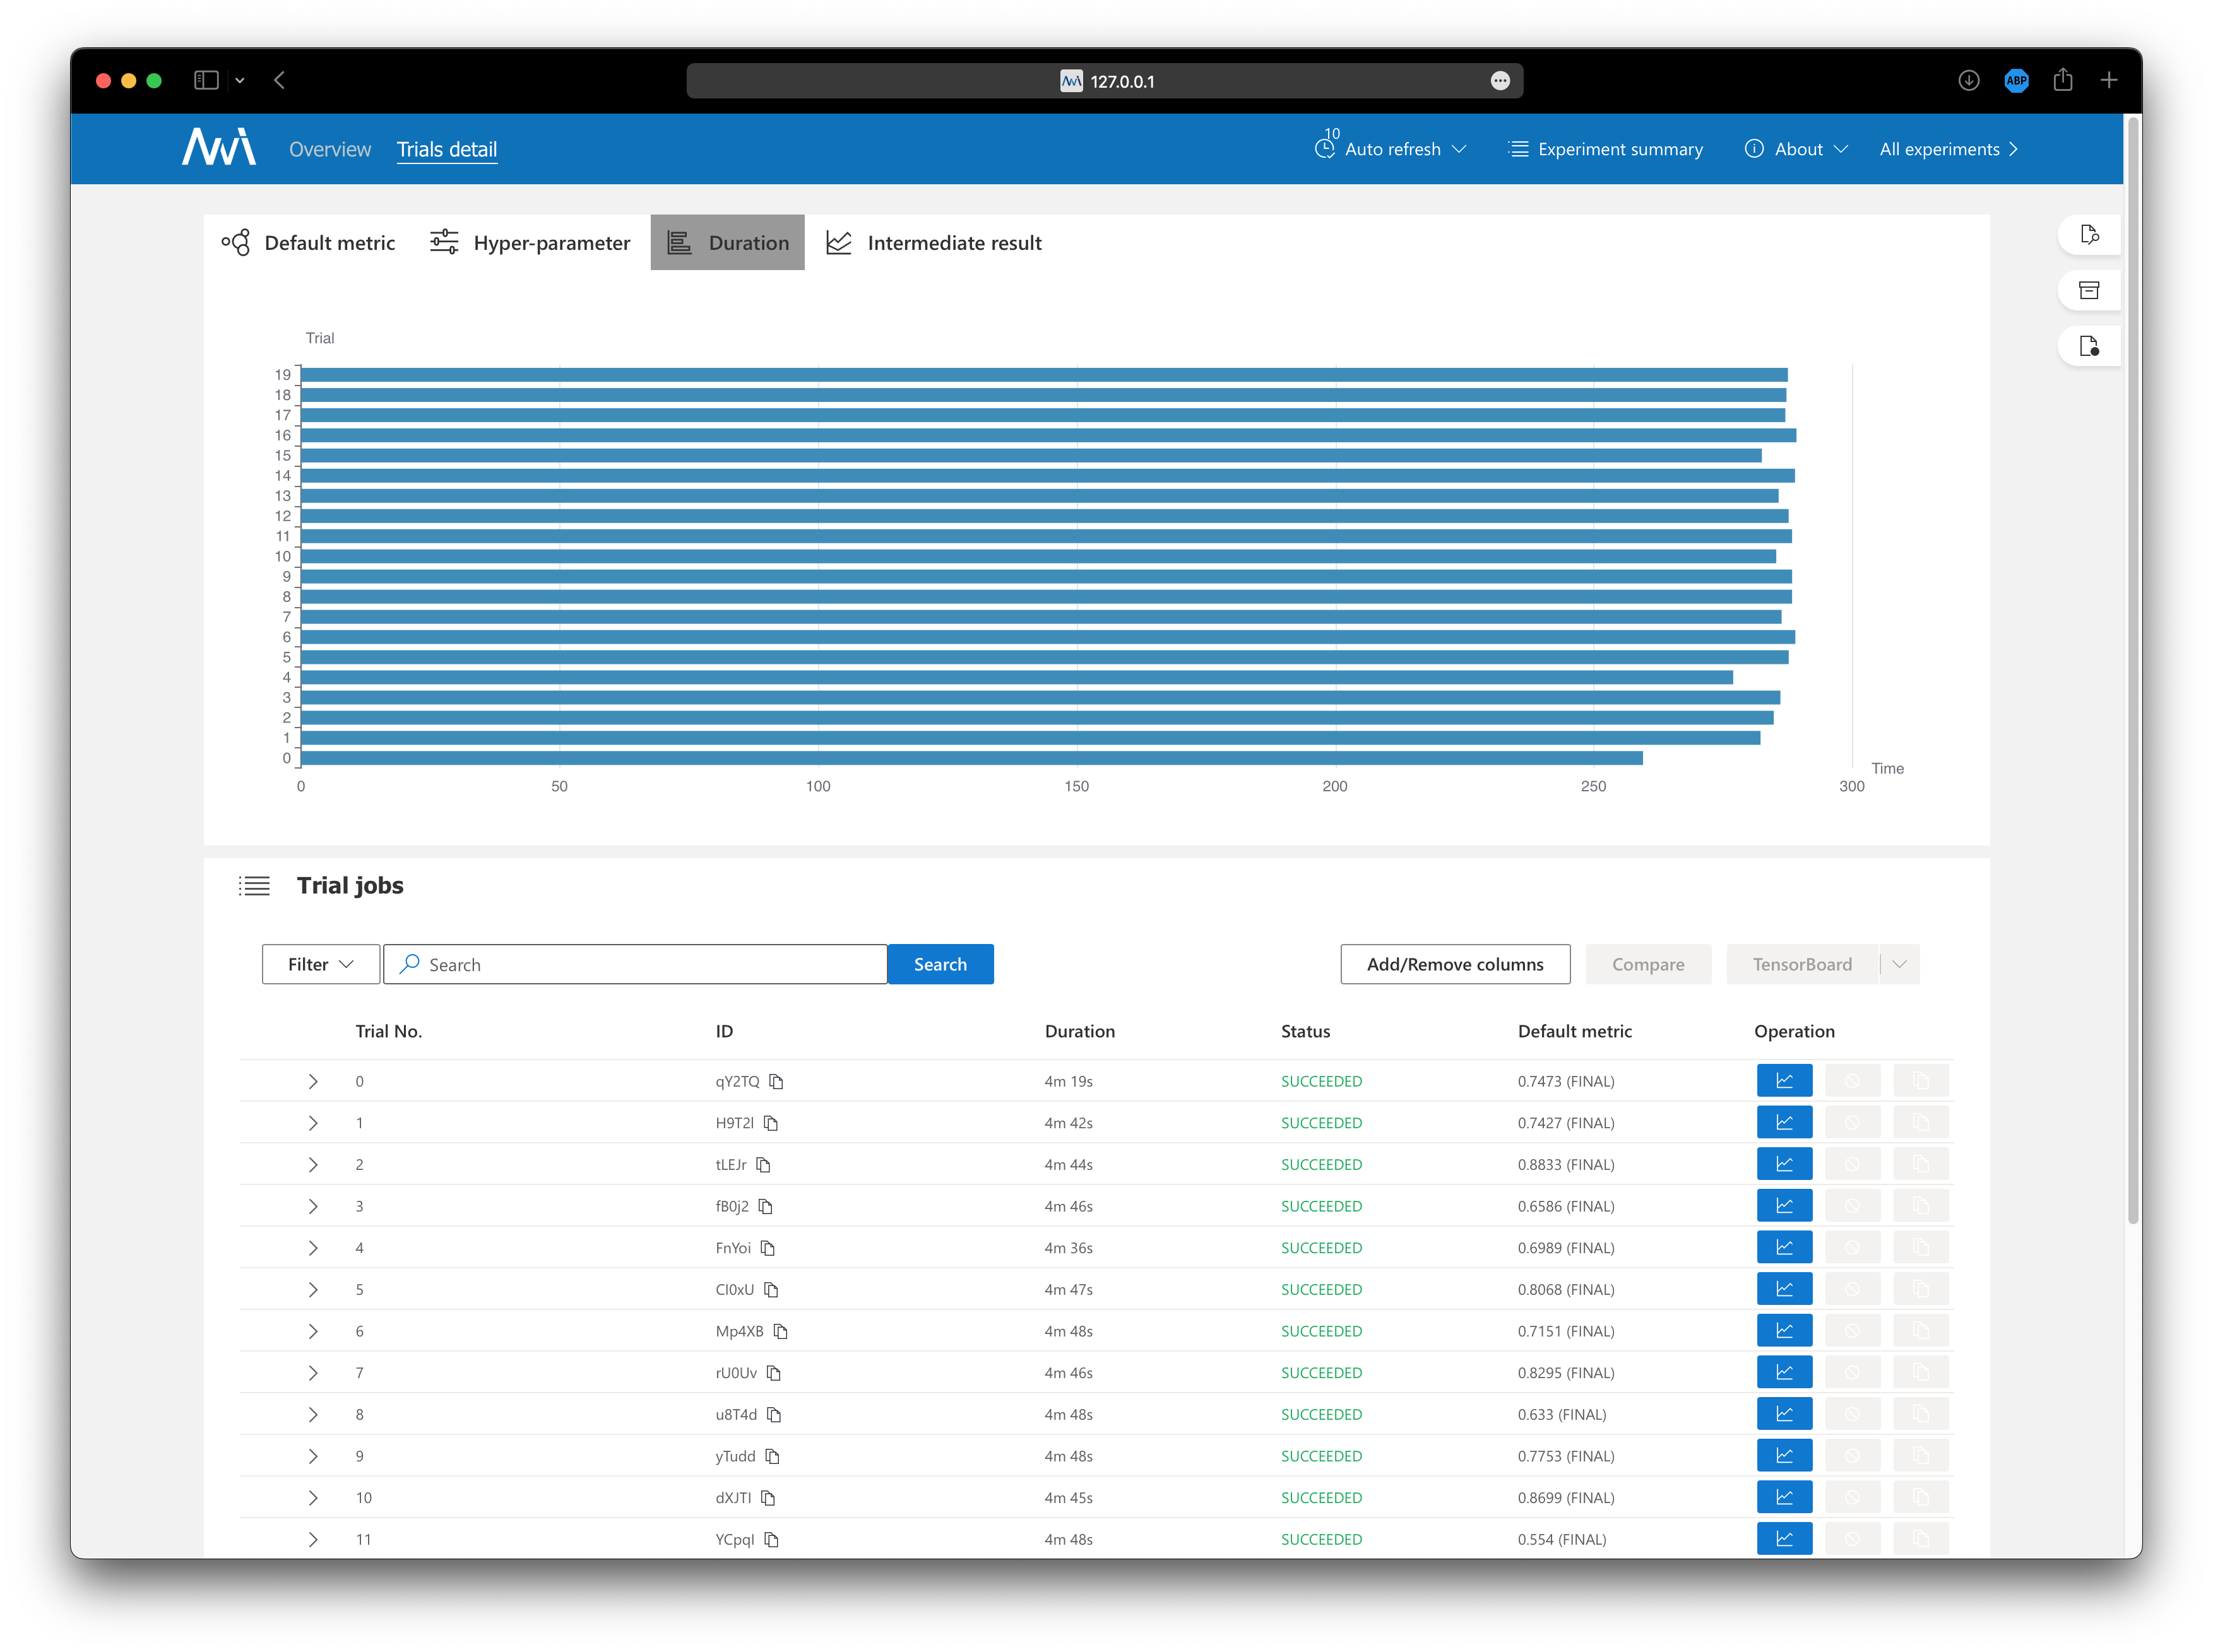
\includegraphics[width=3.5in]{../proj3/figures/mlp_hyperband_latency.png}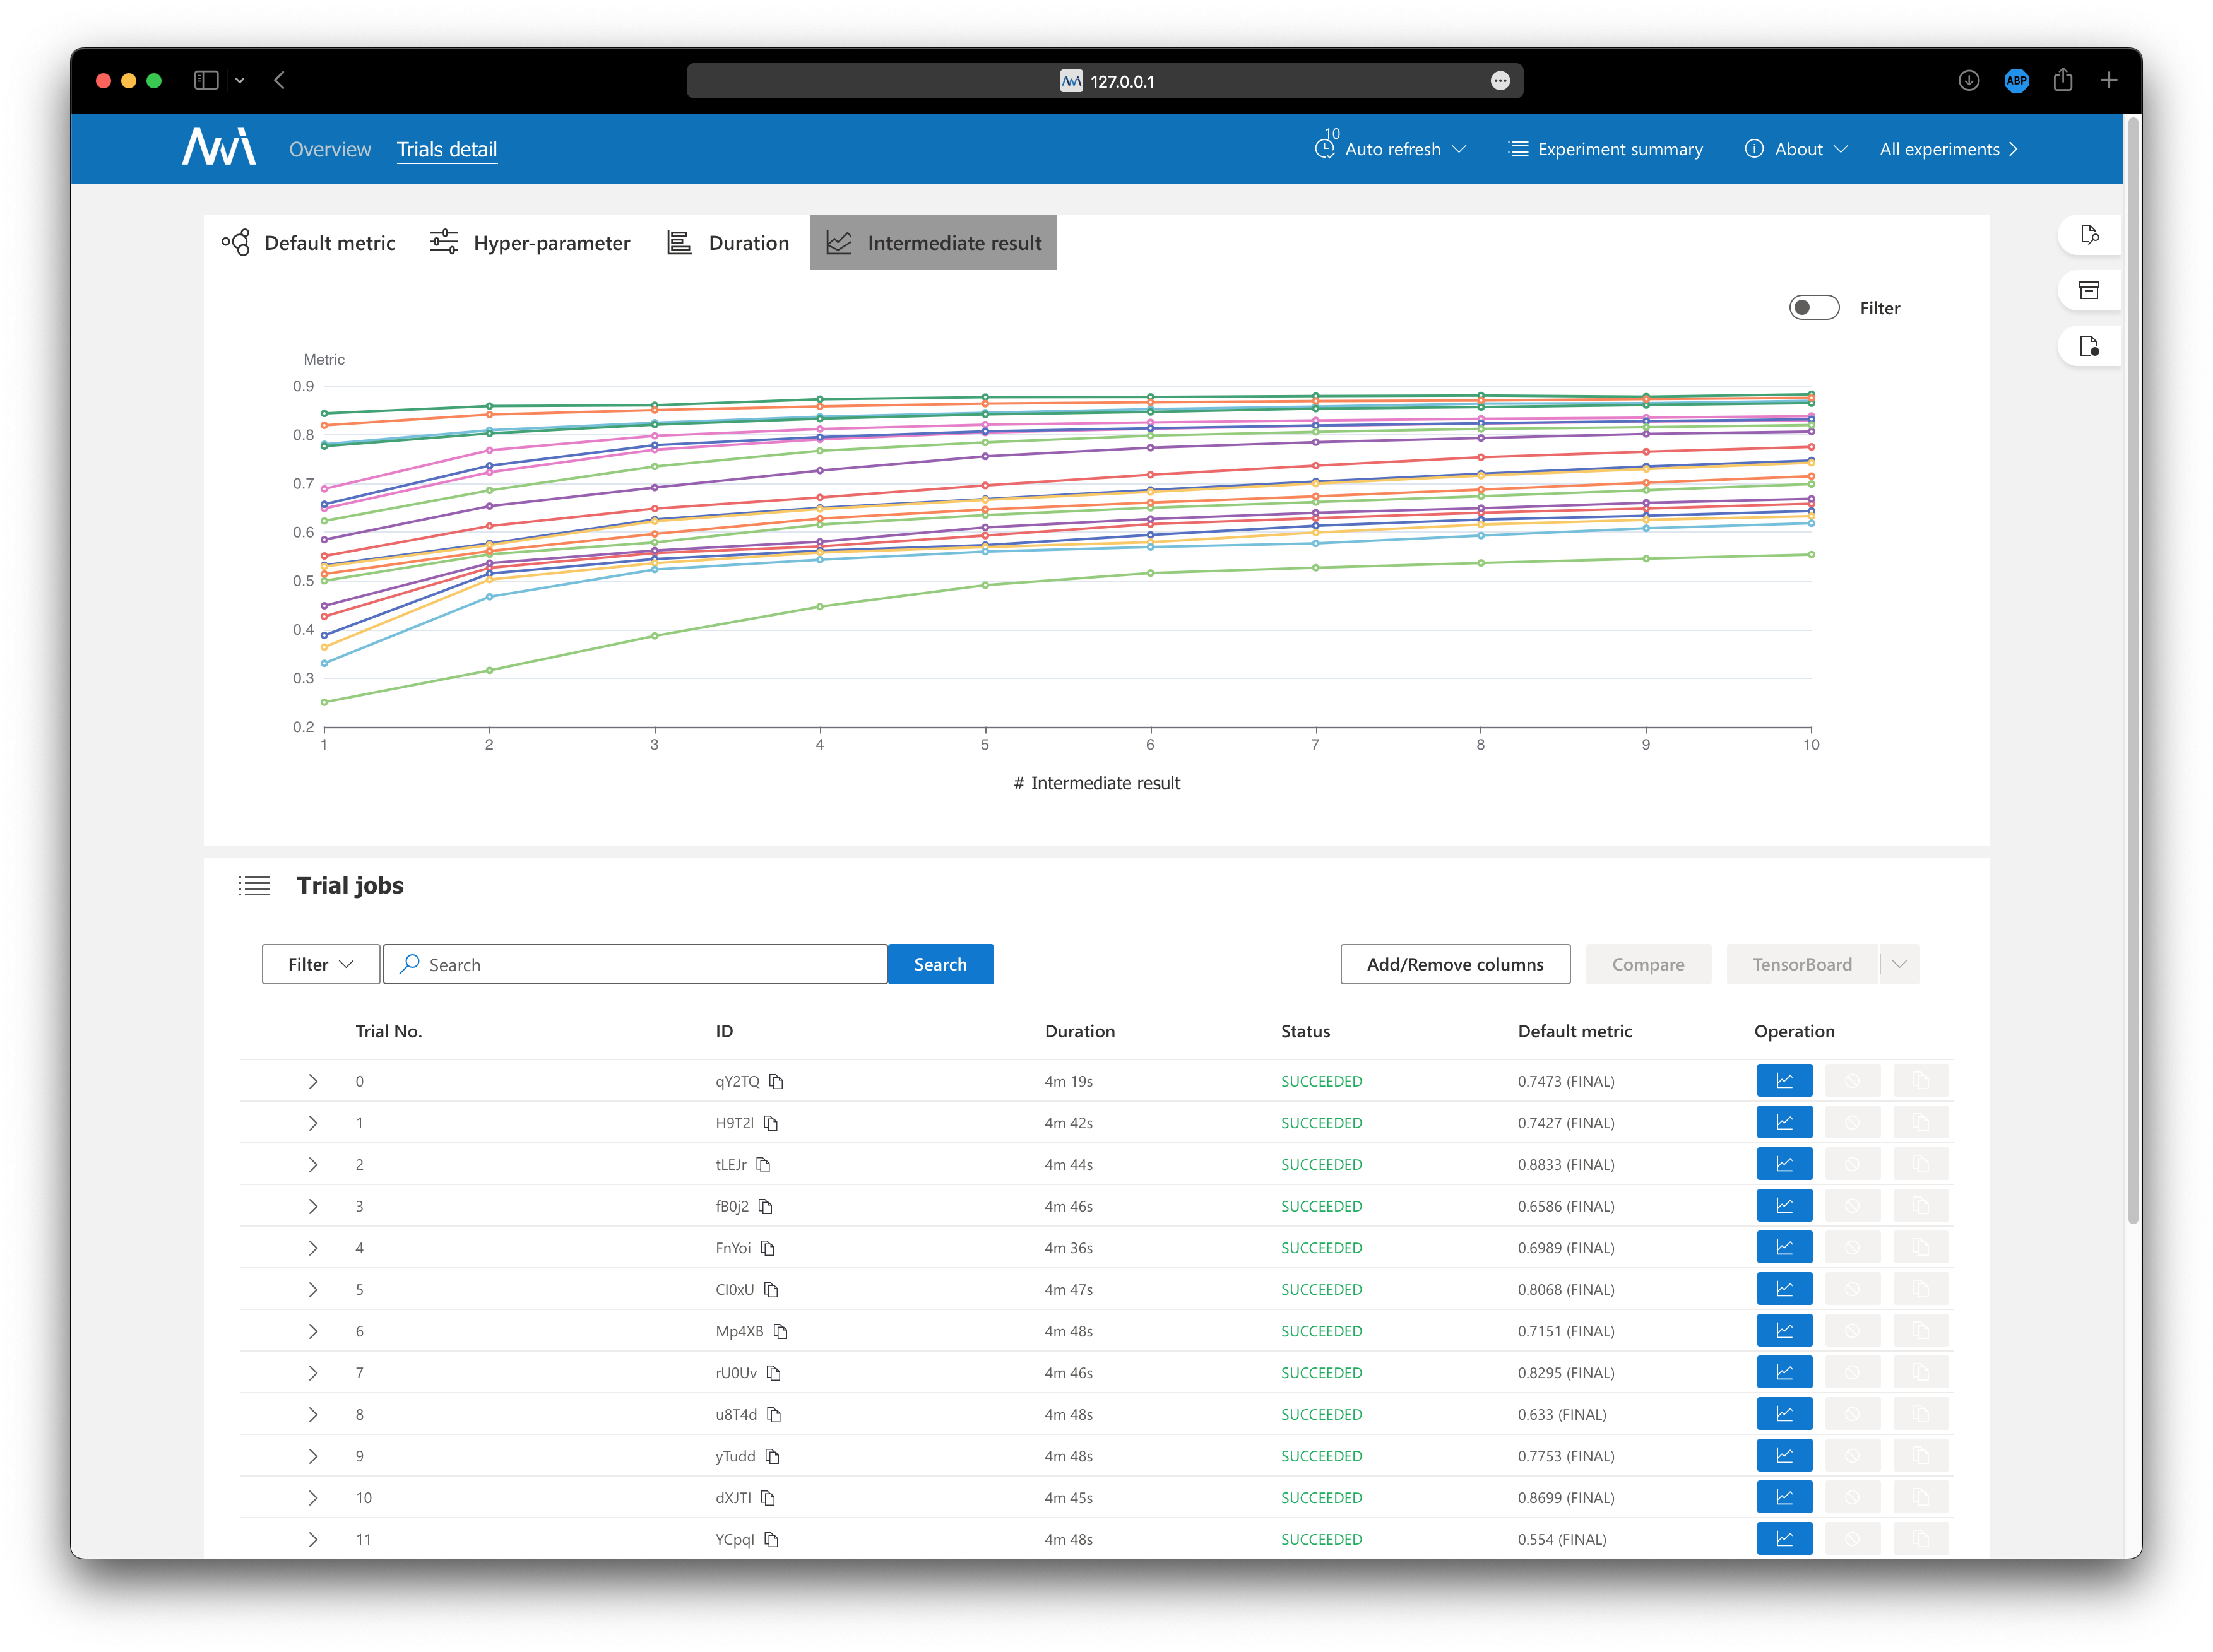
\includegraphics[width=3.5in]{../proj3/figures/mlp_hyperband_intermediate.png}}
    \caption{MLP with Hyperband Tuner on Learning Rate and Momentum}
    \label{fig:mlp-hyperband}
\end{figure}
\begin{figure}
    \centerline{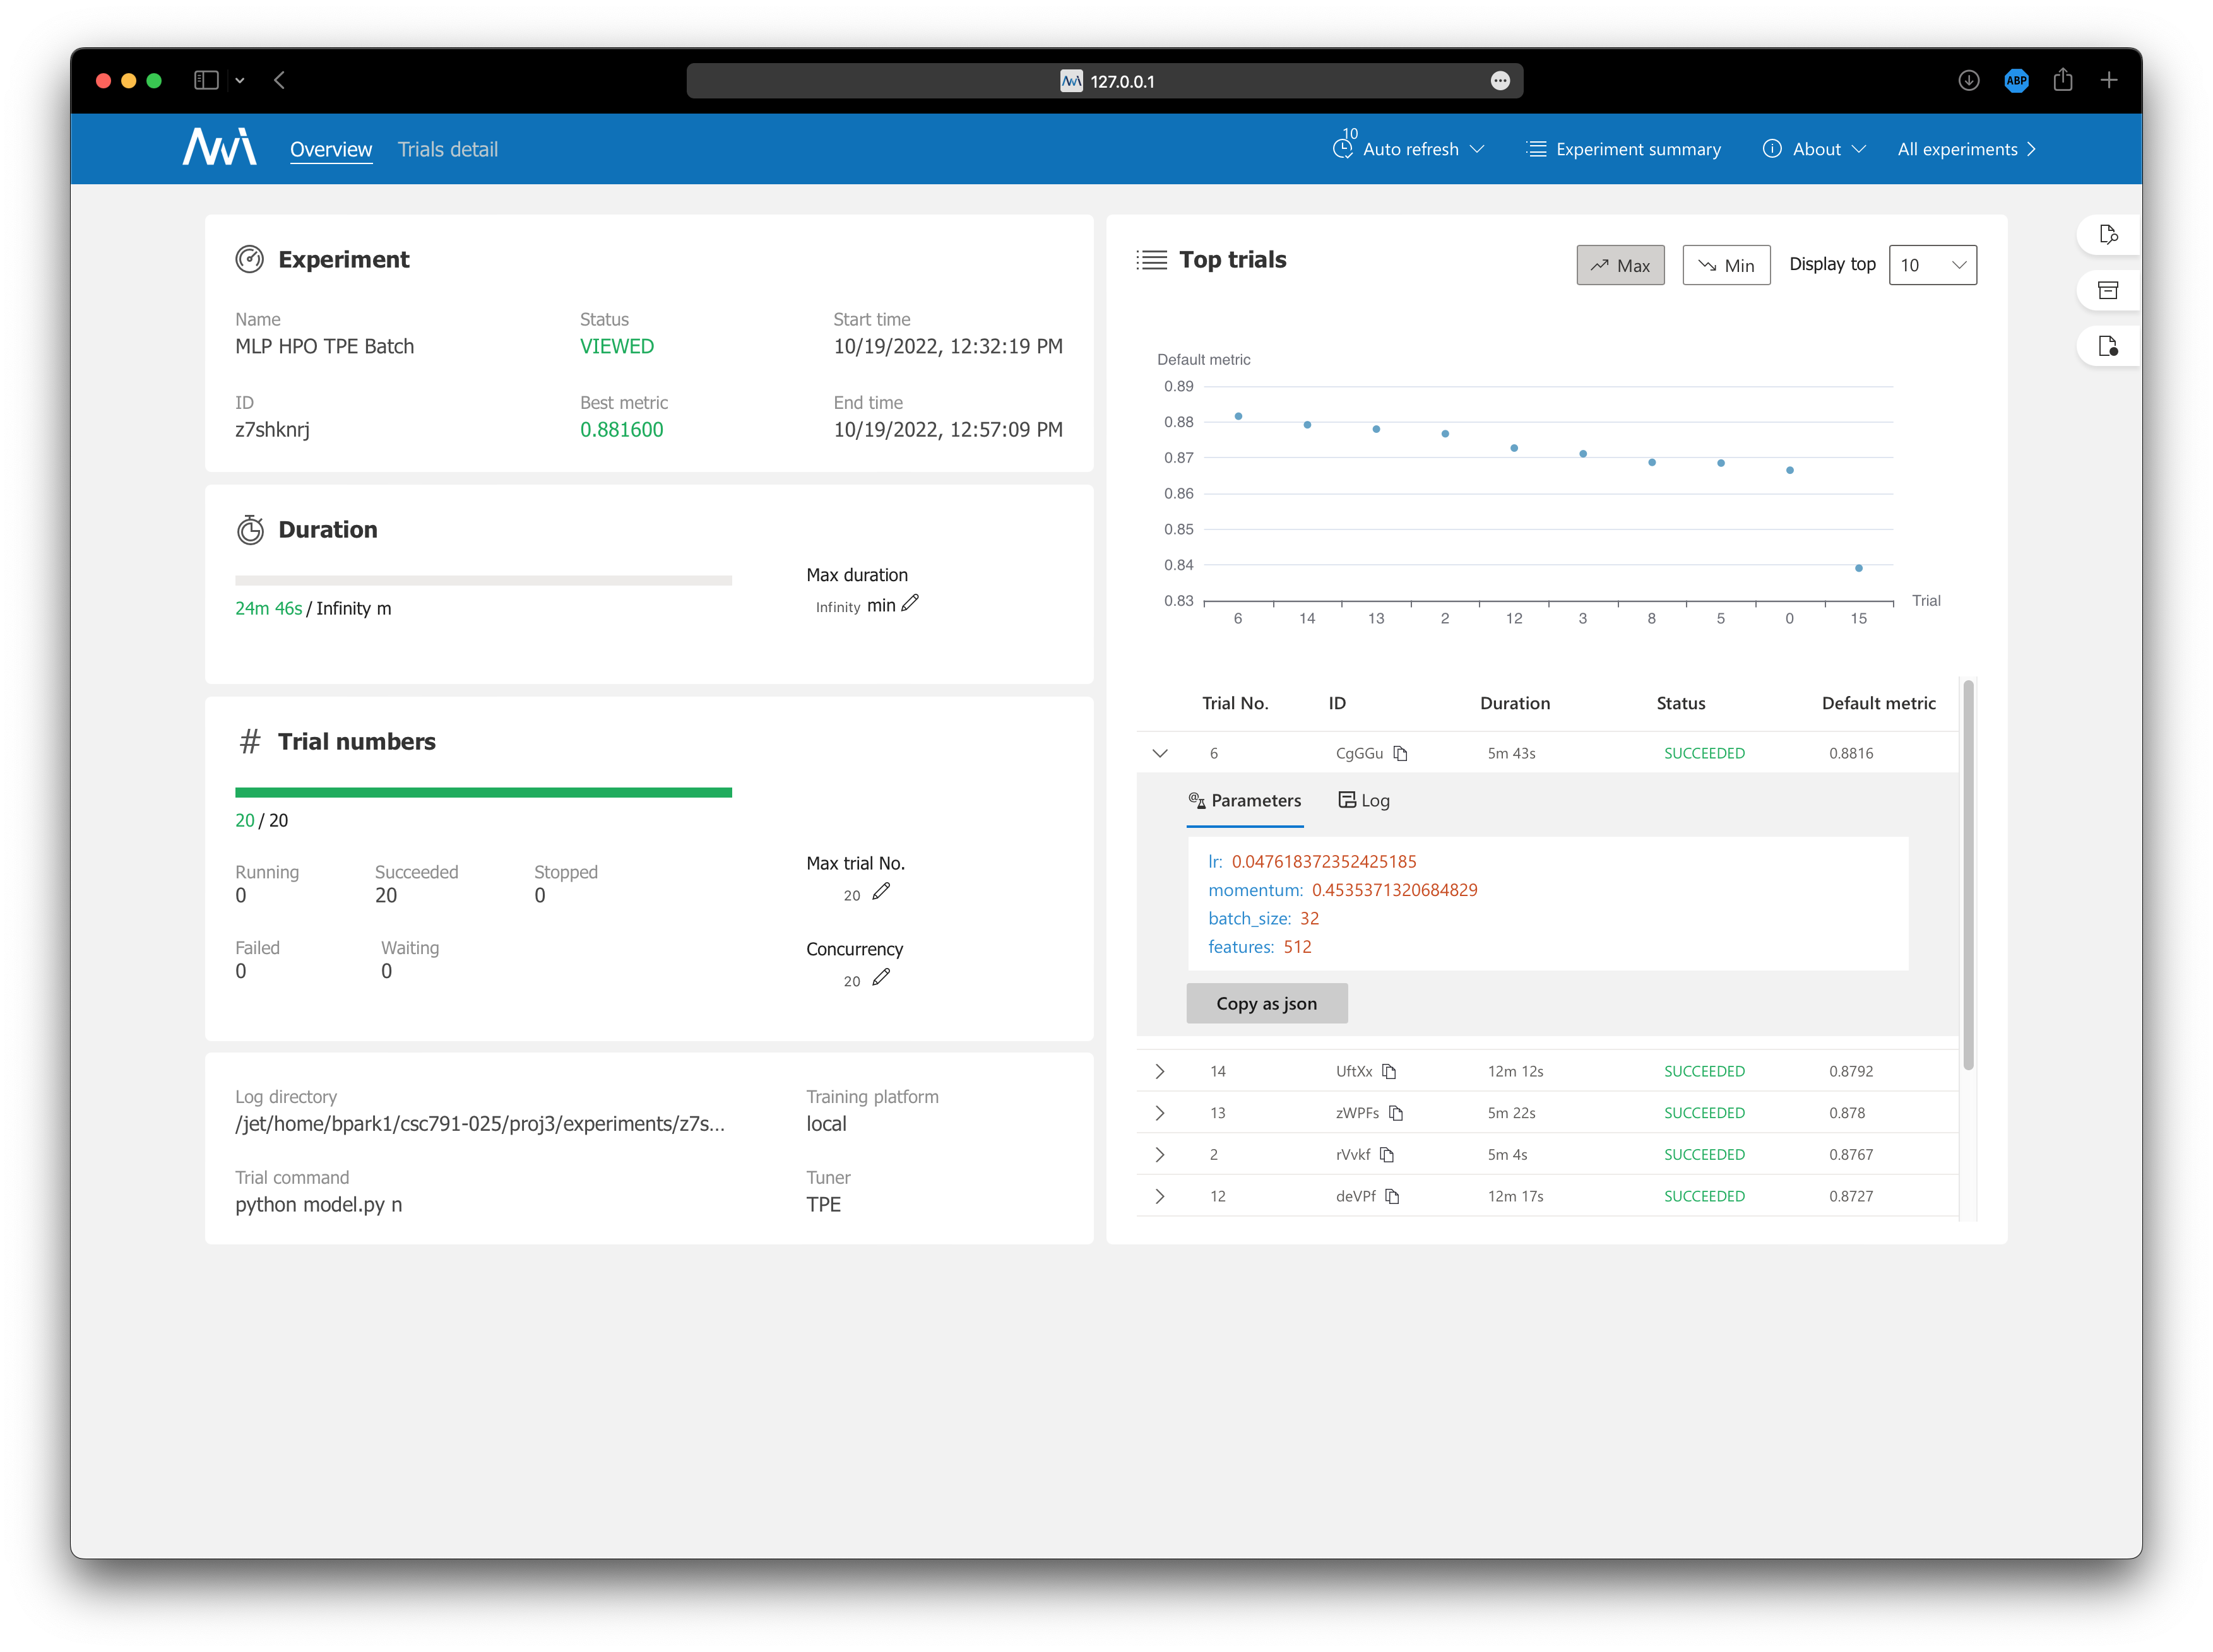
\includegraphics[width=3.5in]{../proj3/figures/mlp_tpe_batch_overview.png}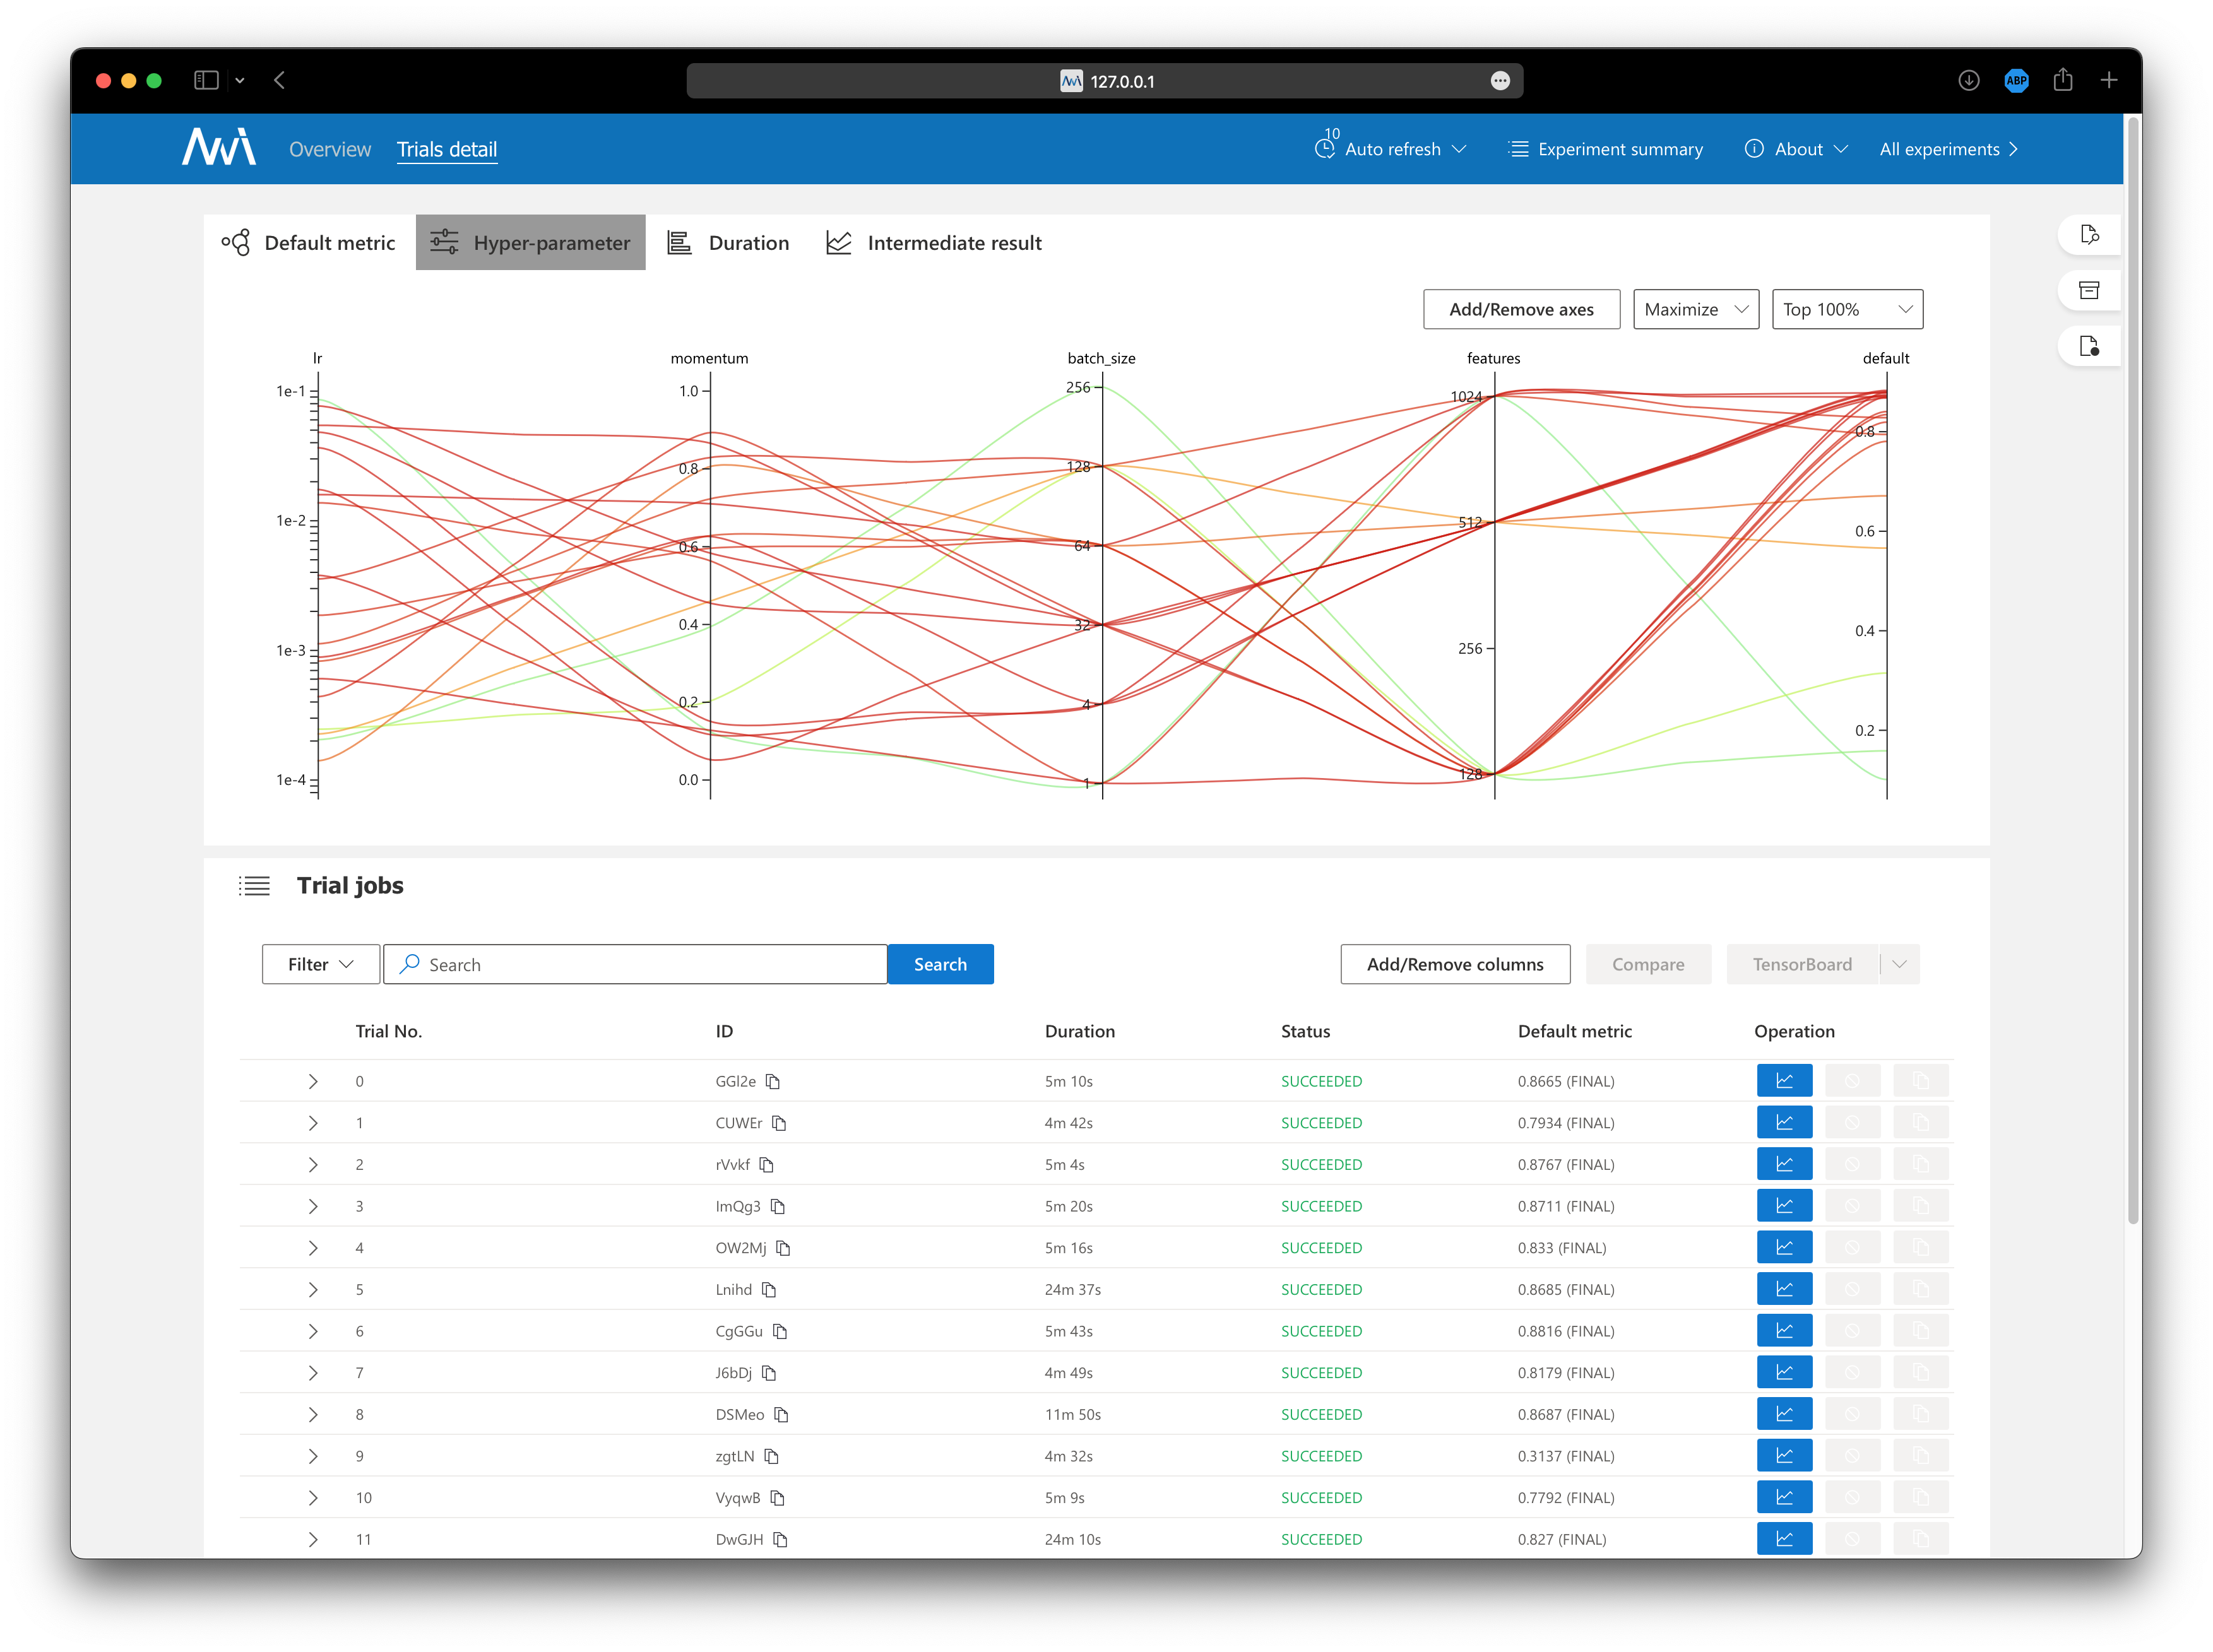
\includegraphics[width=3.5in]{../proj3/figures/mlp_tpe_batch_hyperparameter.png}}
    \centerline{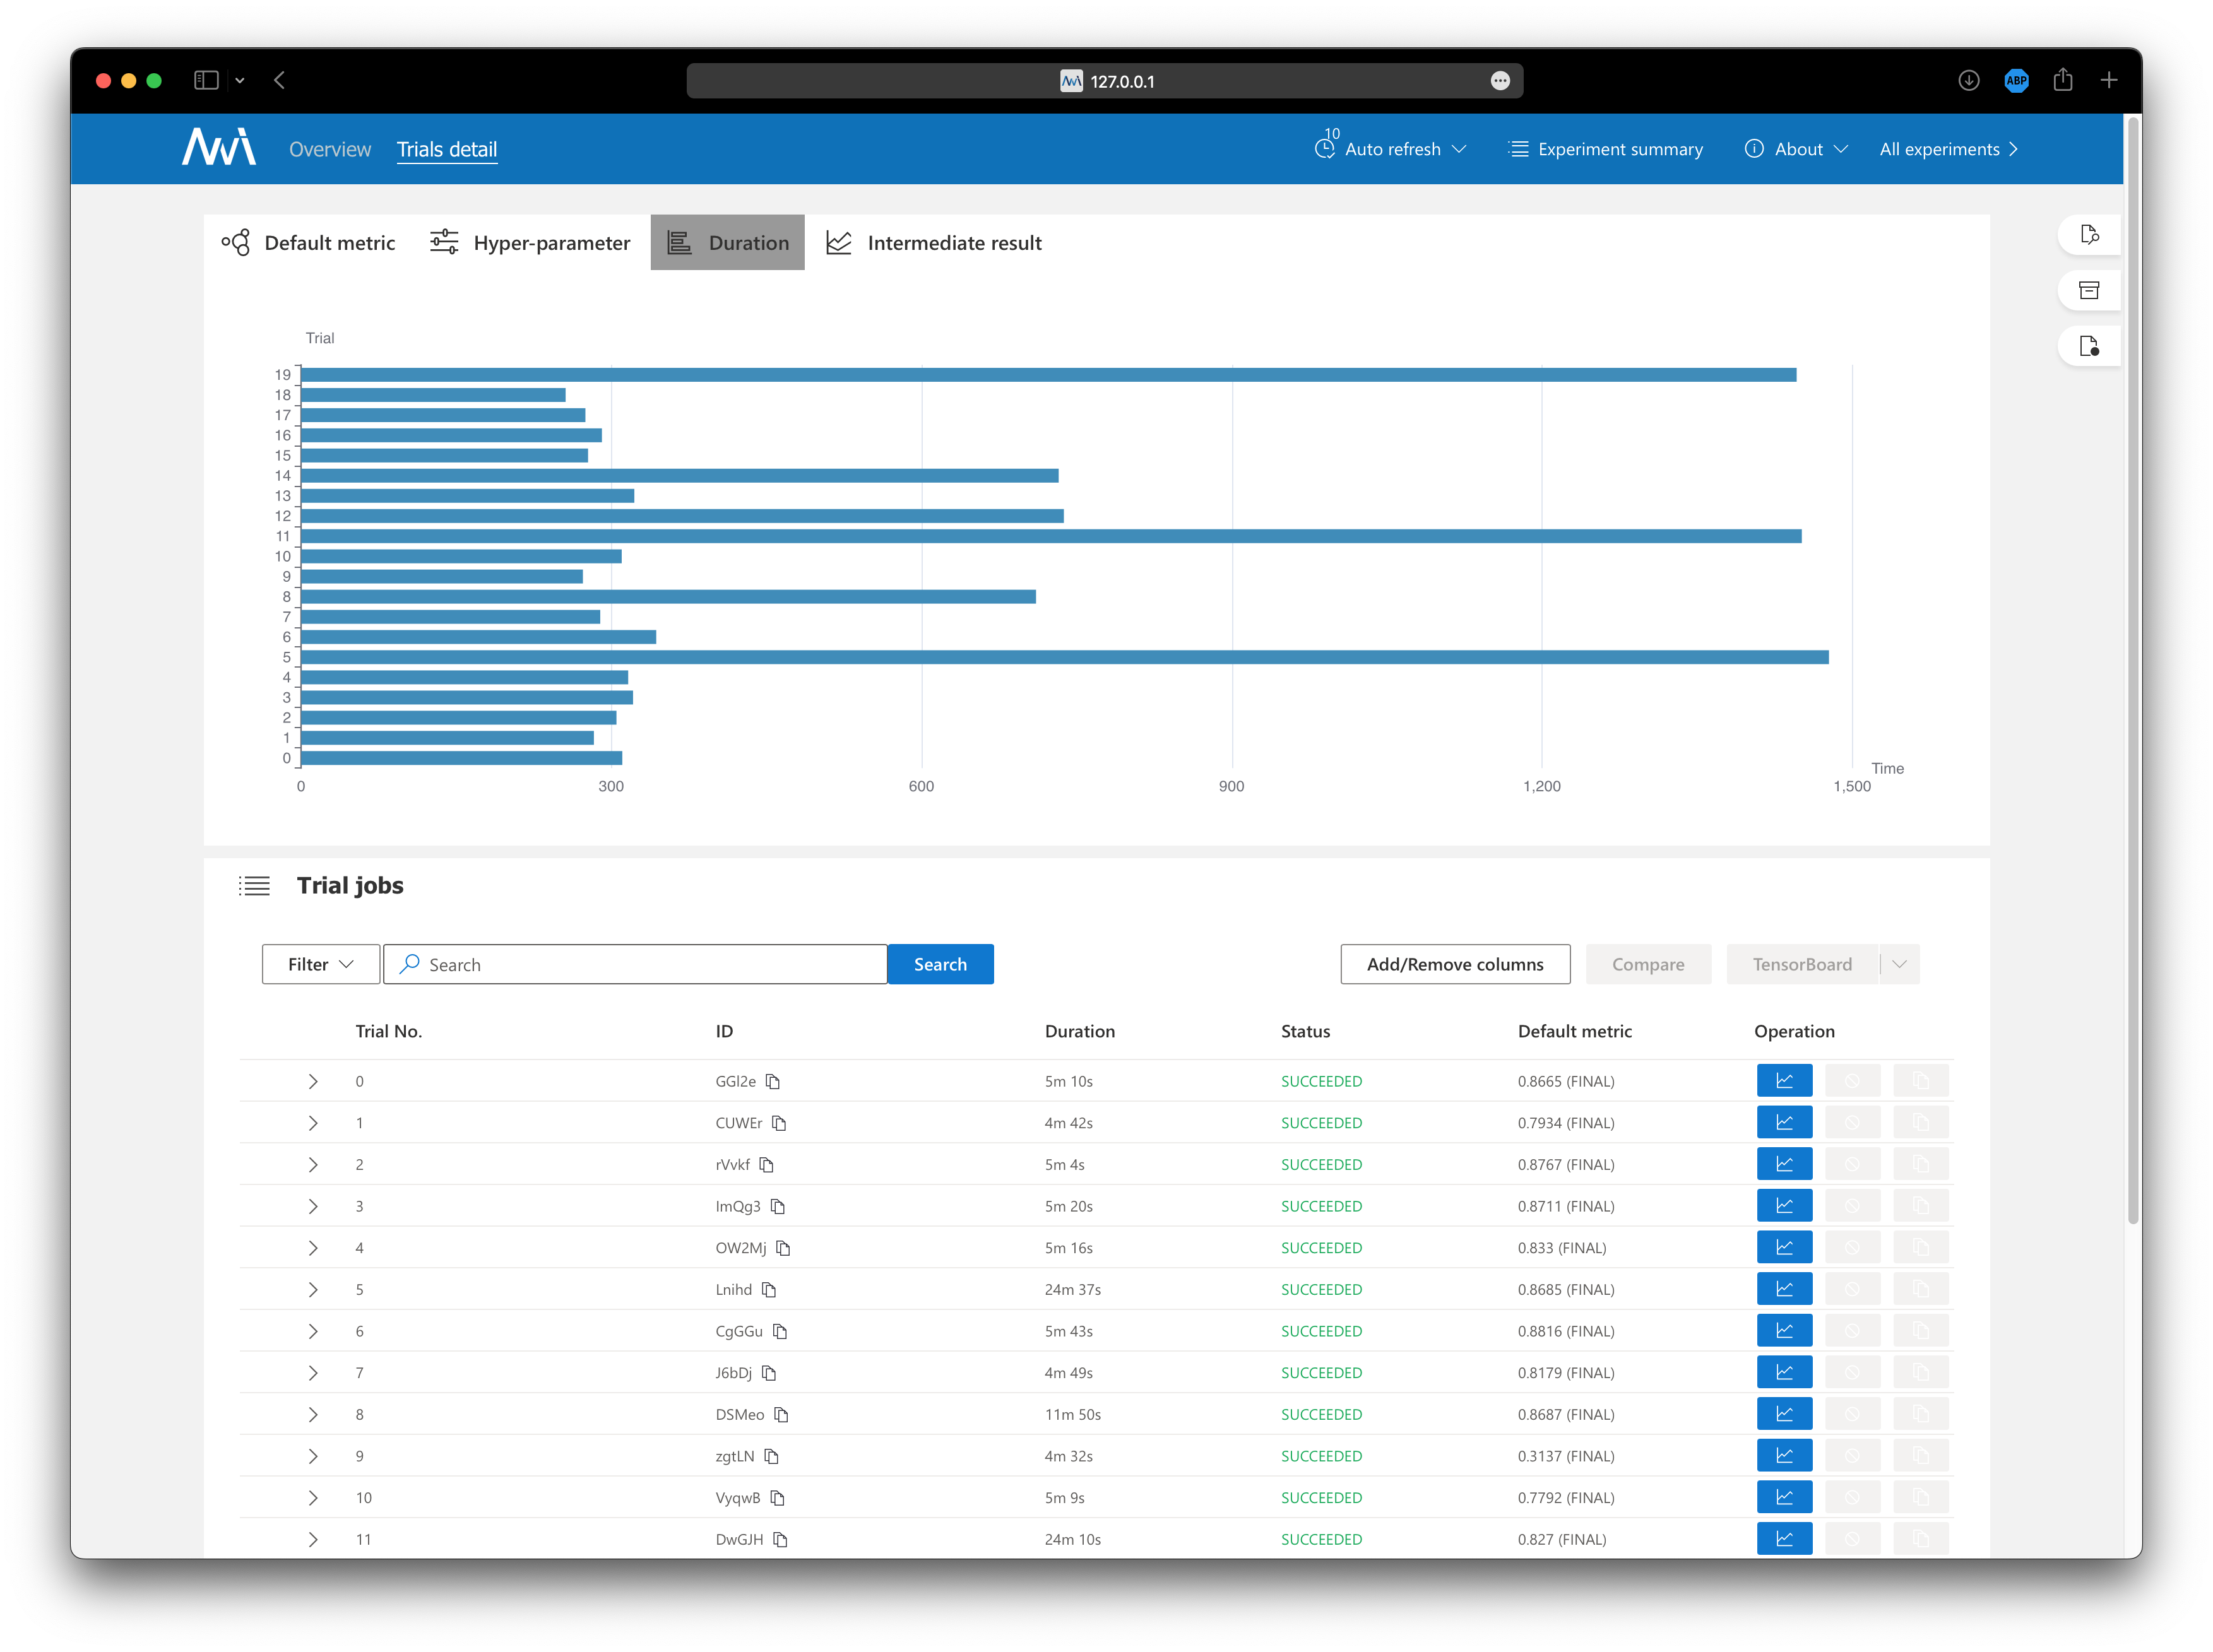
\includegraphics[width=3.5in]{../proj3/figures/mlp_tpe_batch_latency.png}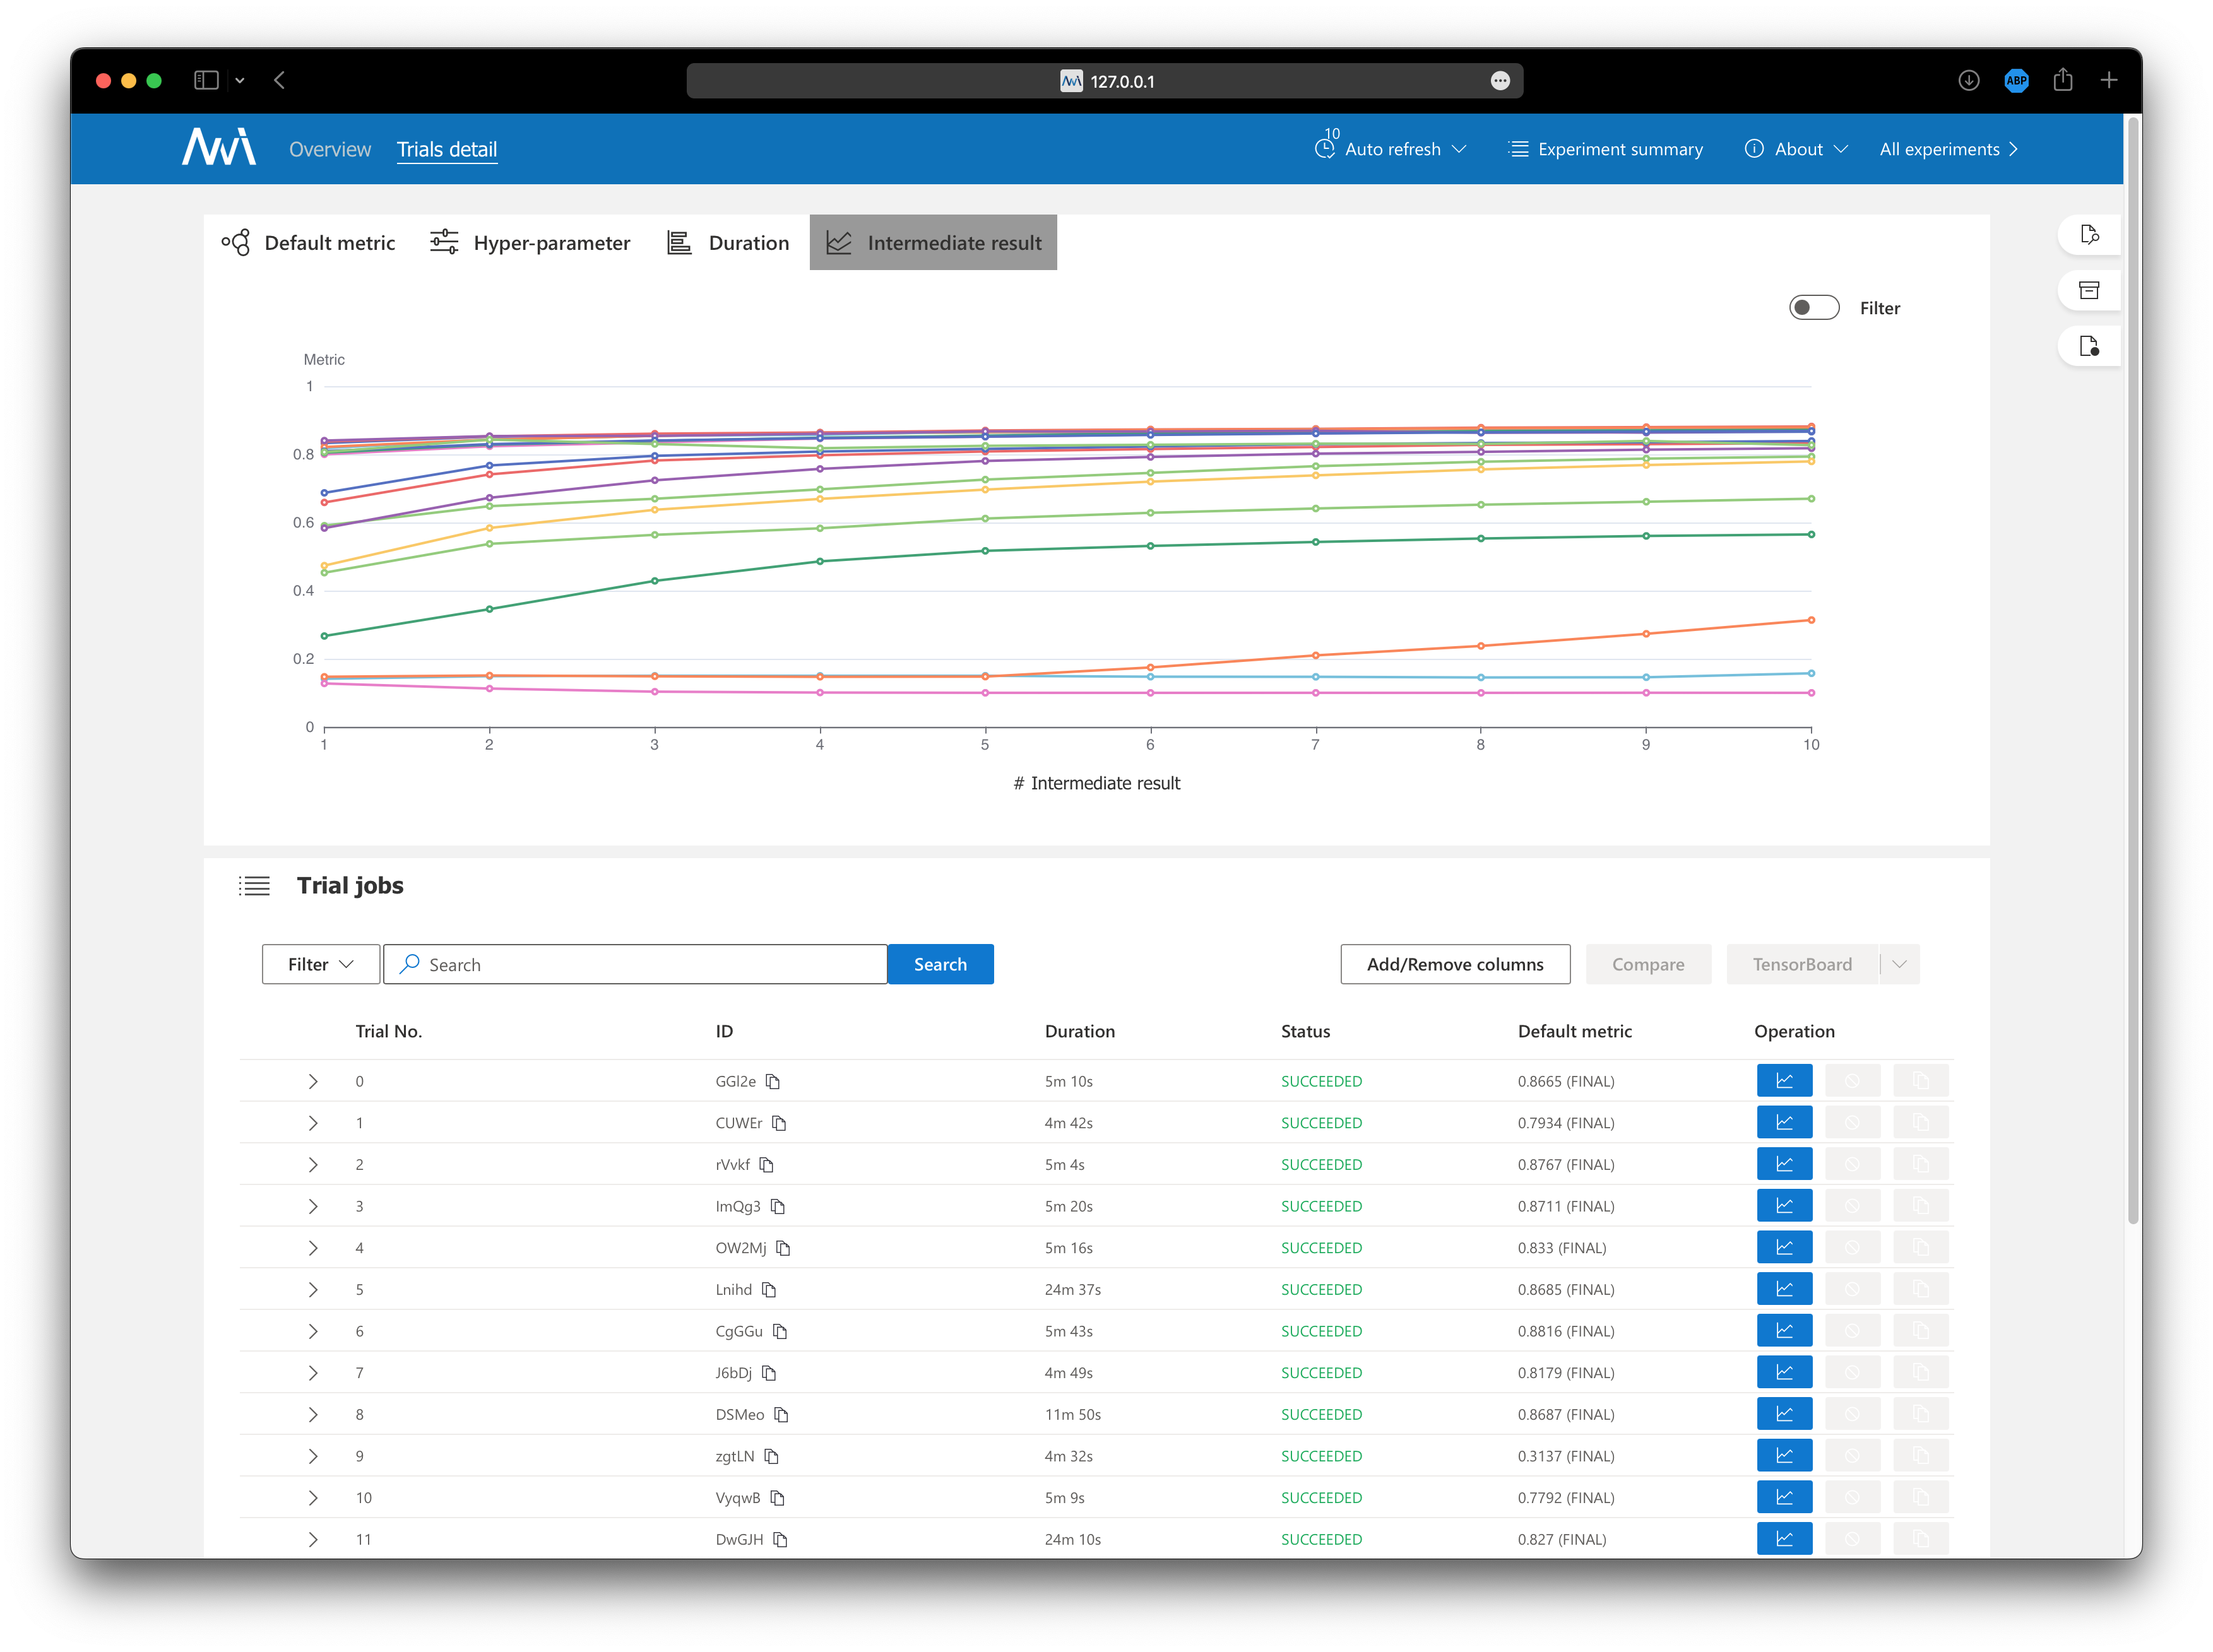
\includegraphics[width=3.5in]{../proj3/figures/mlp_tpe_batch_intermediate.png}}
    \caption{MLP with TPE Tuner on Learning Rate, Momentum, Feature Size, and Batch Size}
    \label{fig:mlp-tpe-batch}
\end{figure}
\begin{figure}
    \centerline{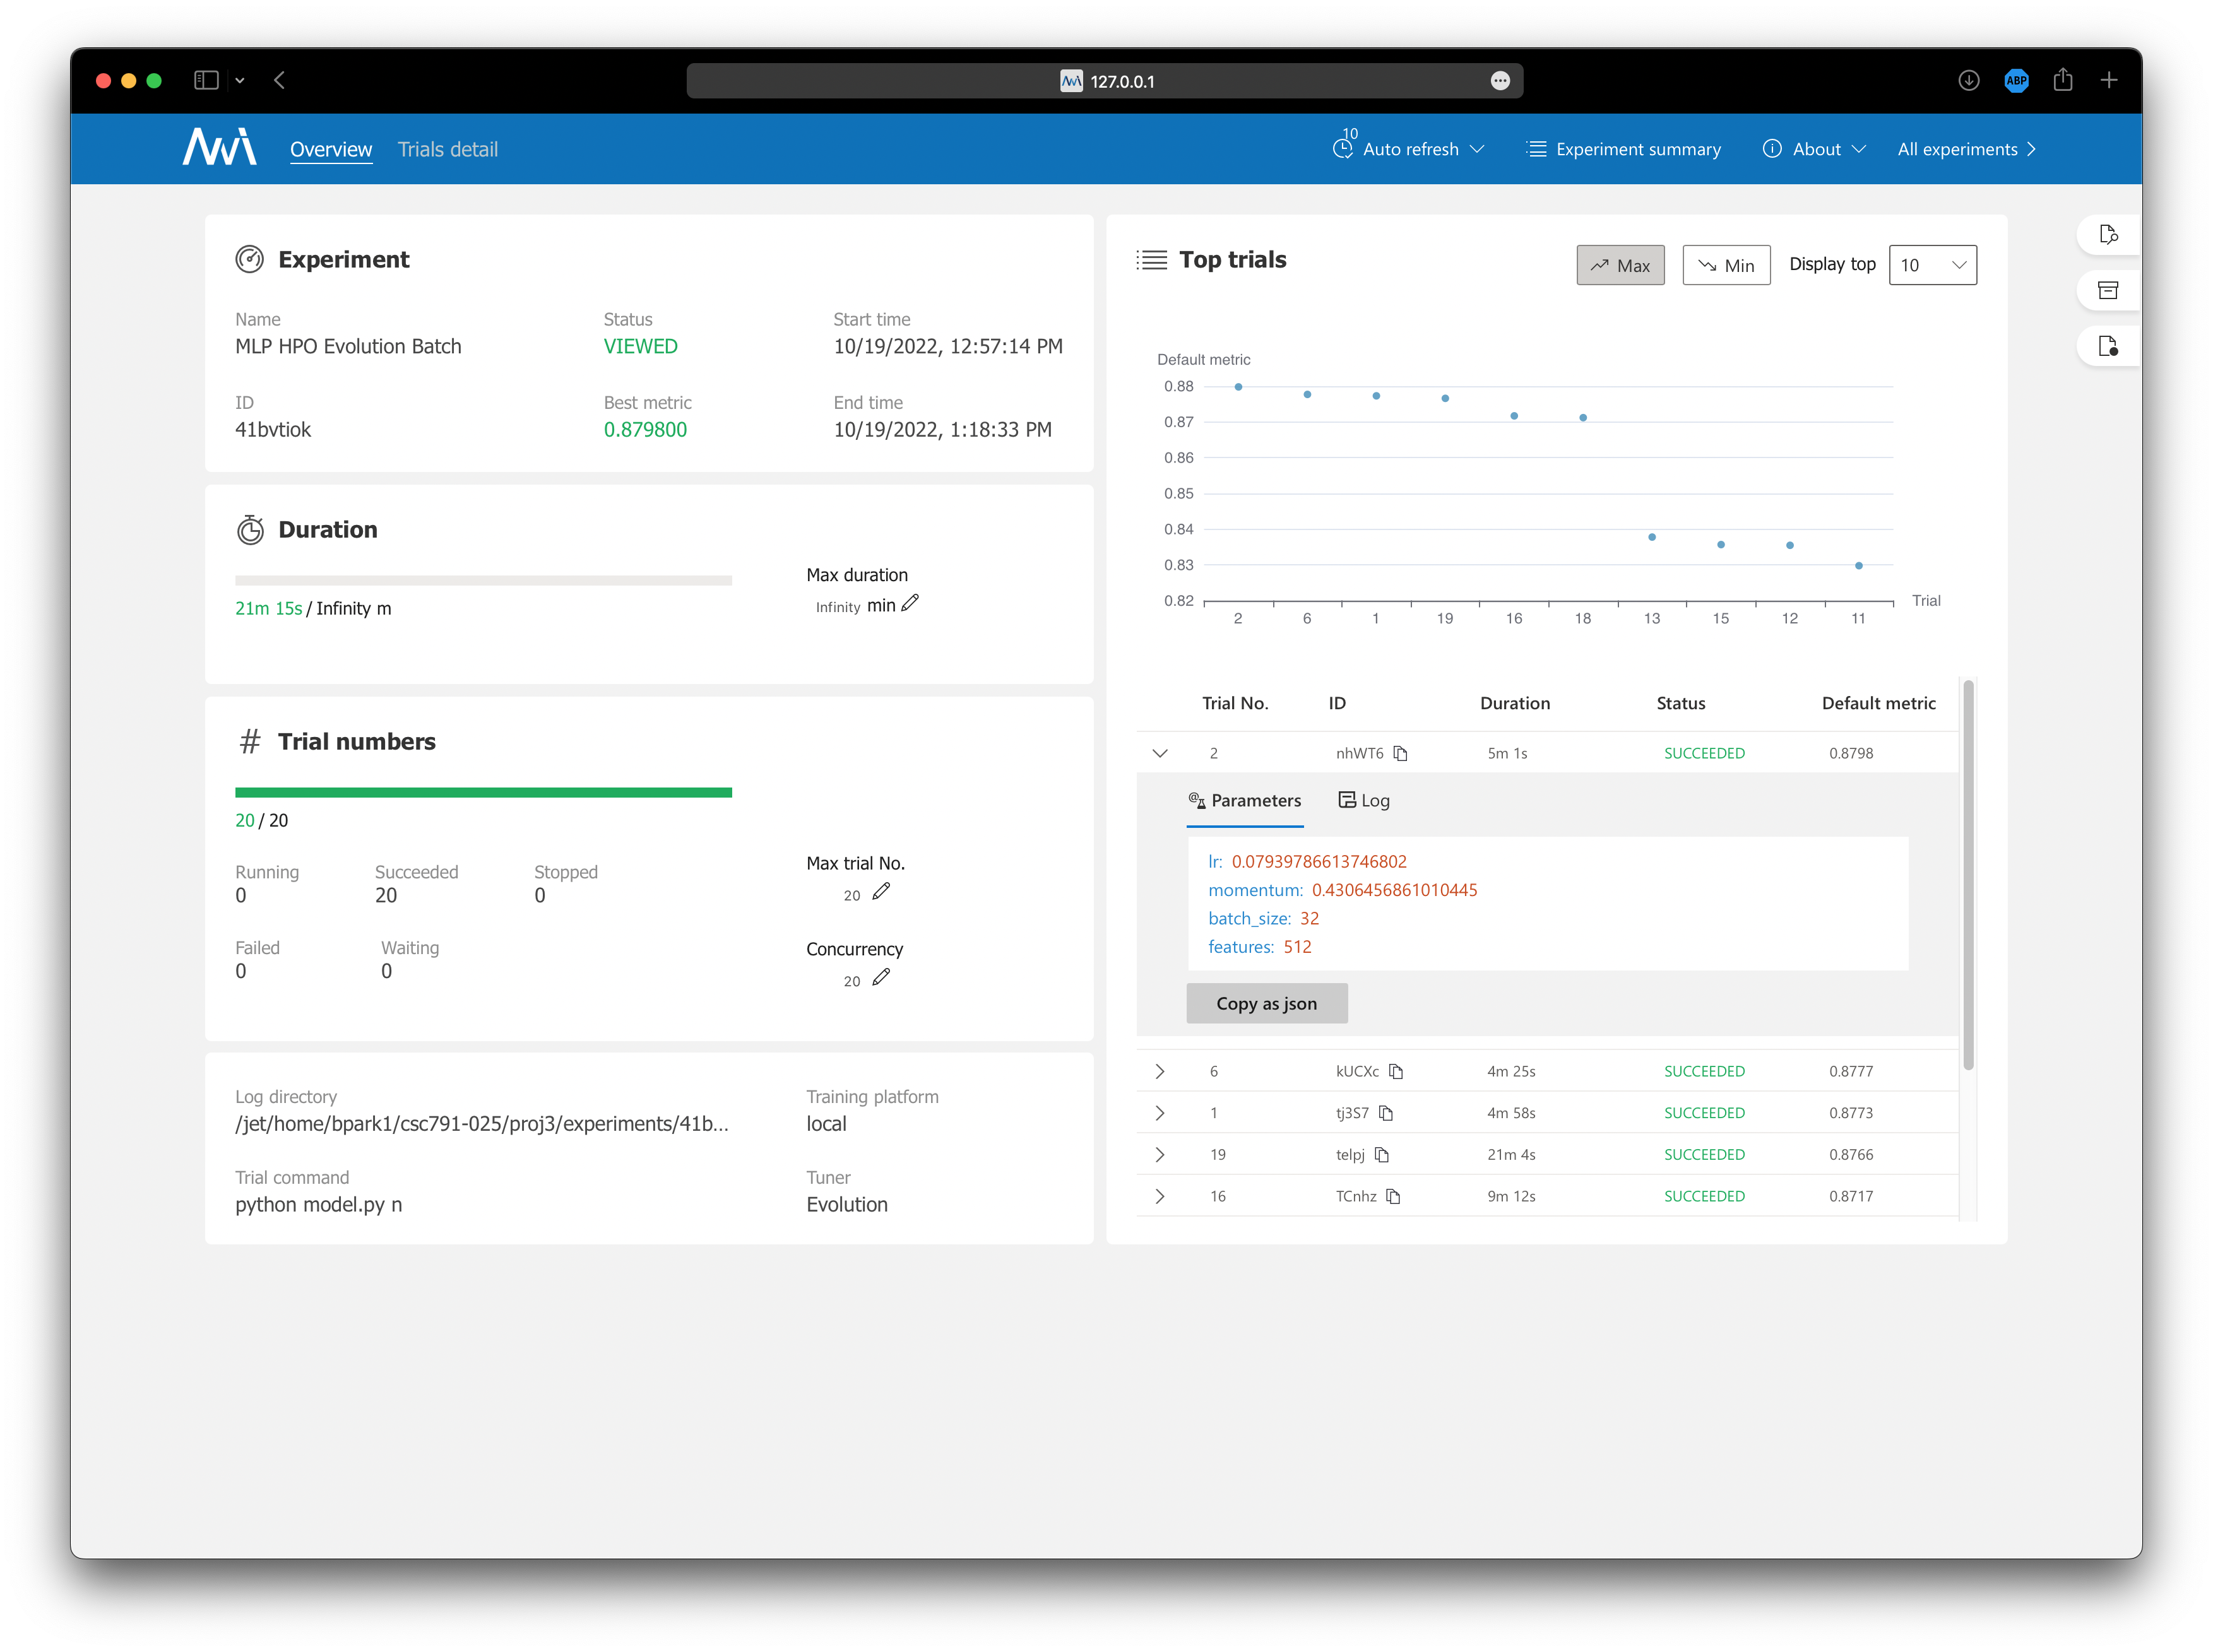
\includegraphics[width=3.5in]{../proj3/figures/mlp_evolution_batch_overview.png}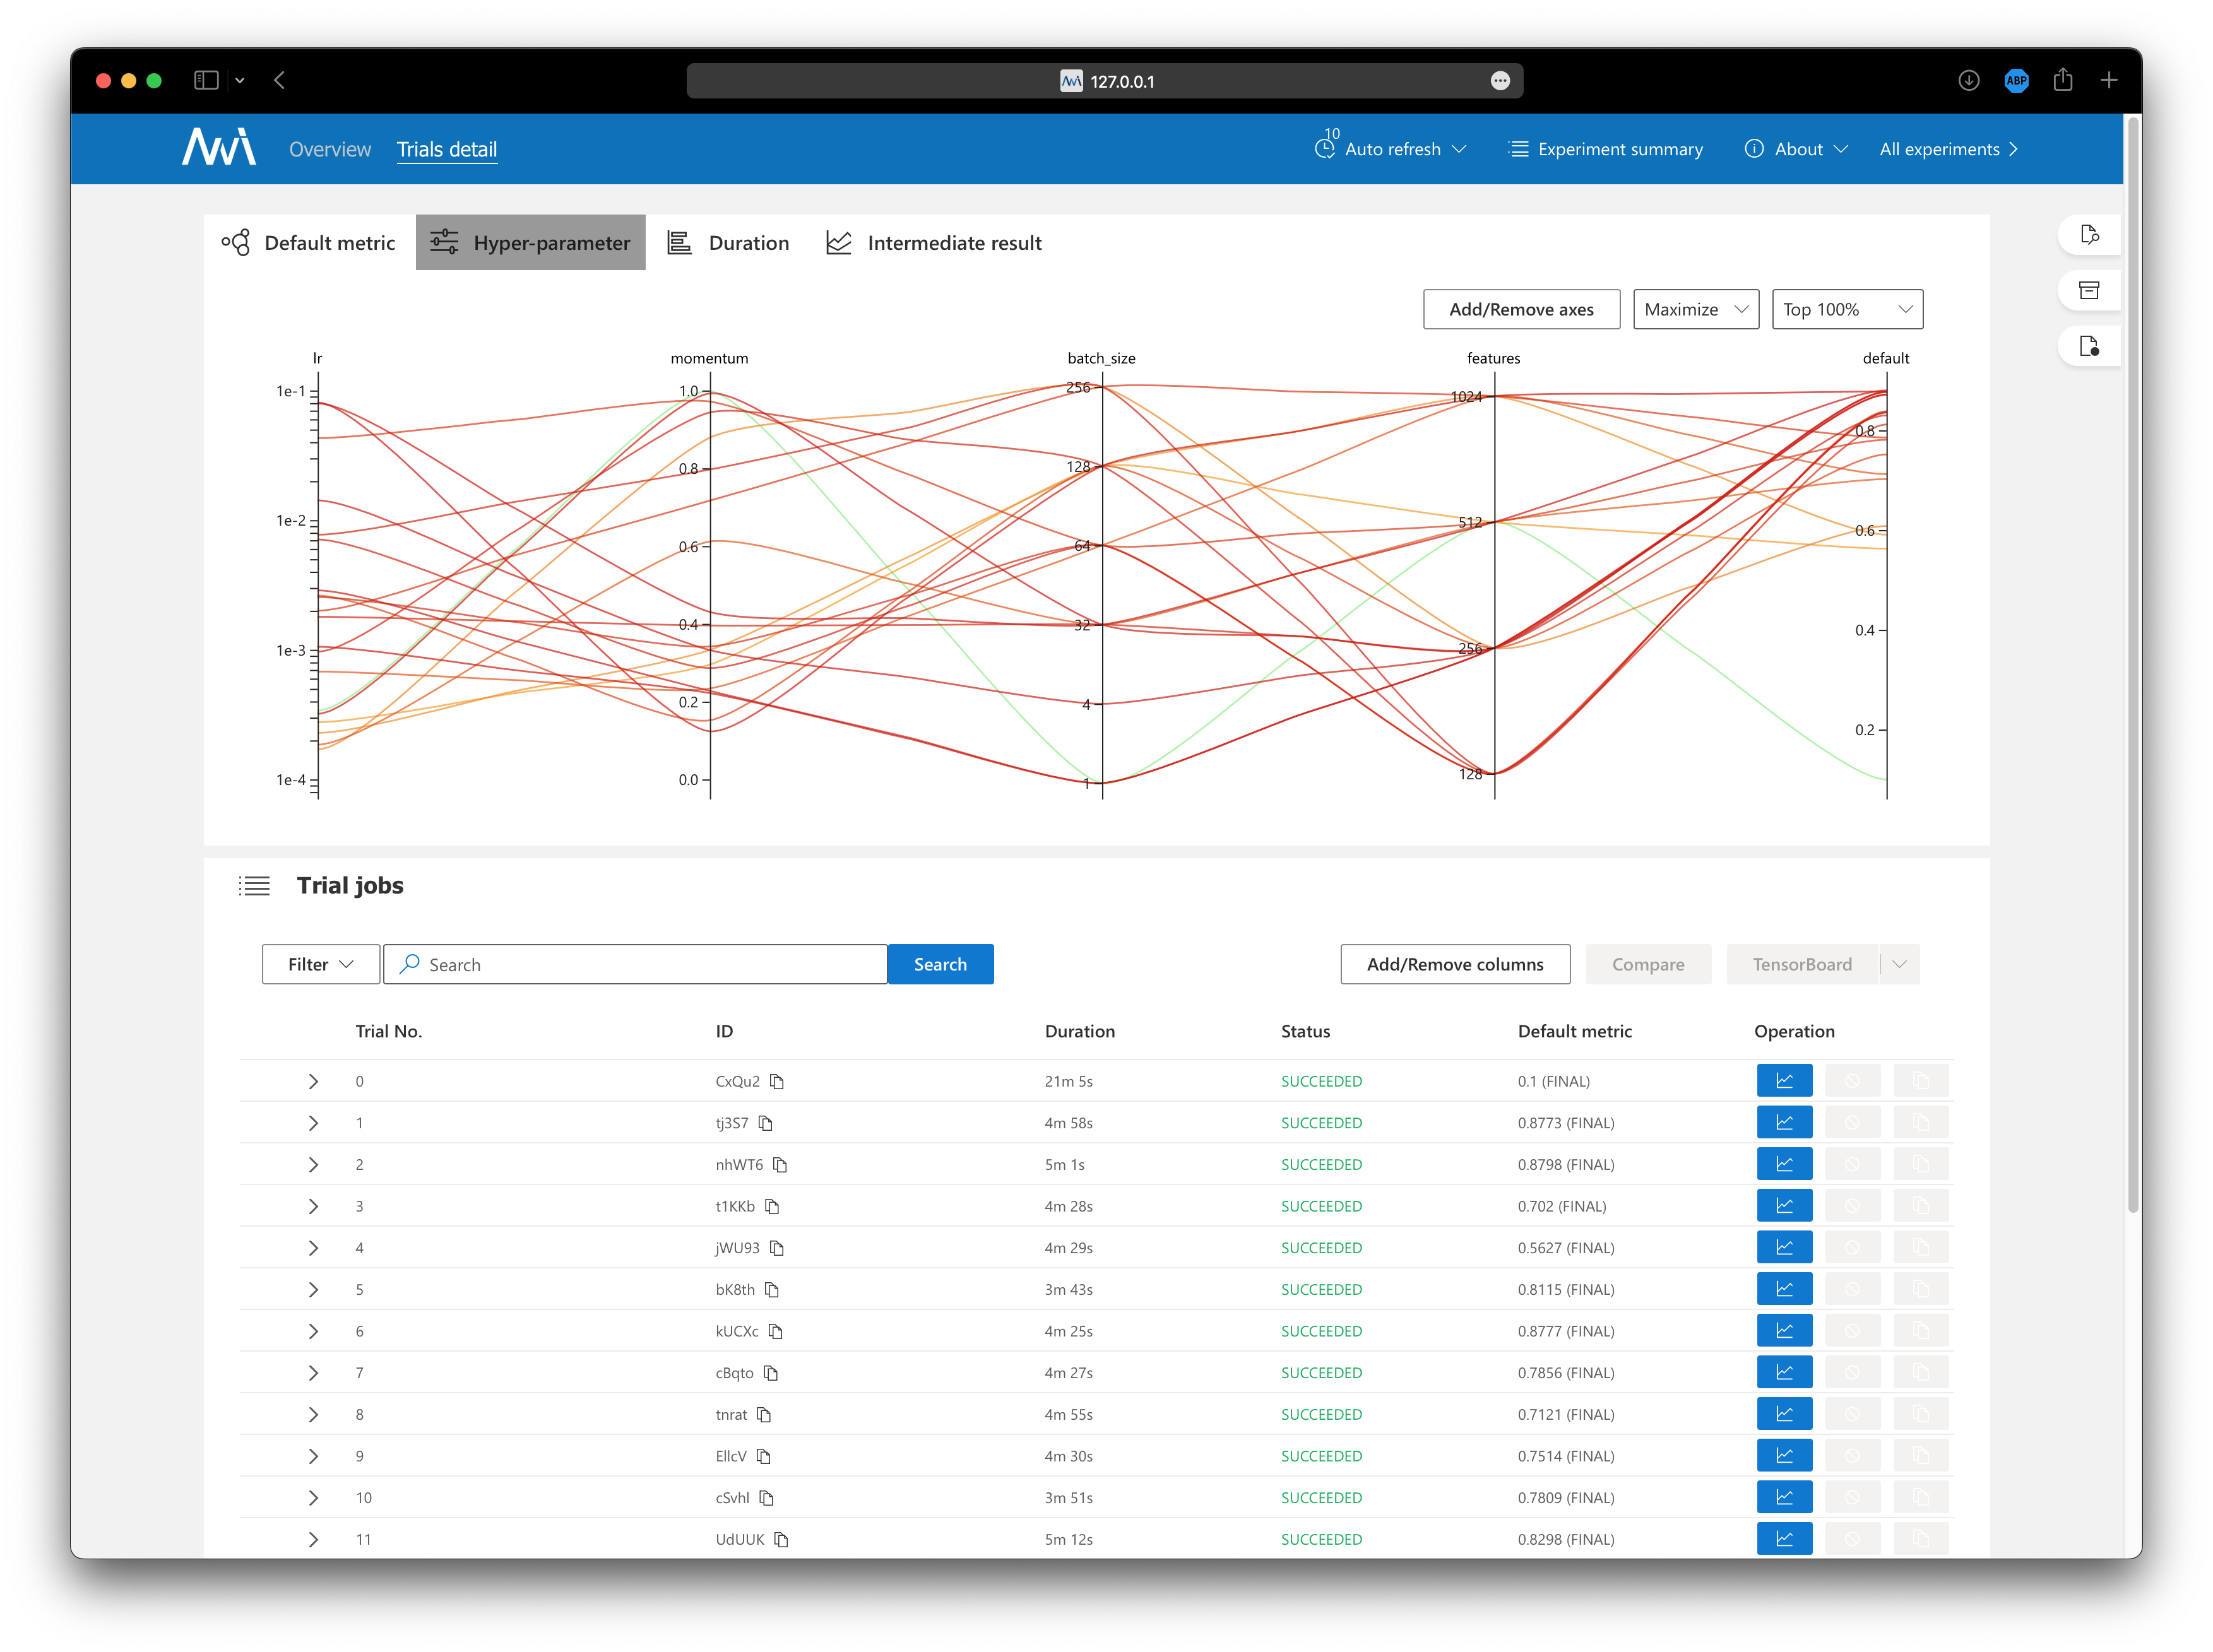
\includegraphics[width=3.5in]{../proj3/figures/mlp_evolution_batch_hyperparameter.png}}
    \centerline{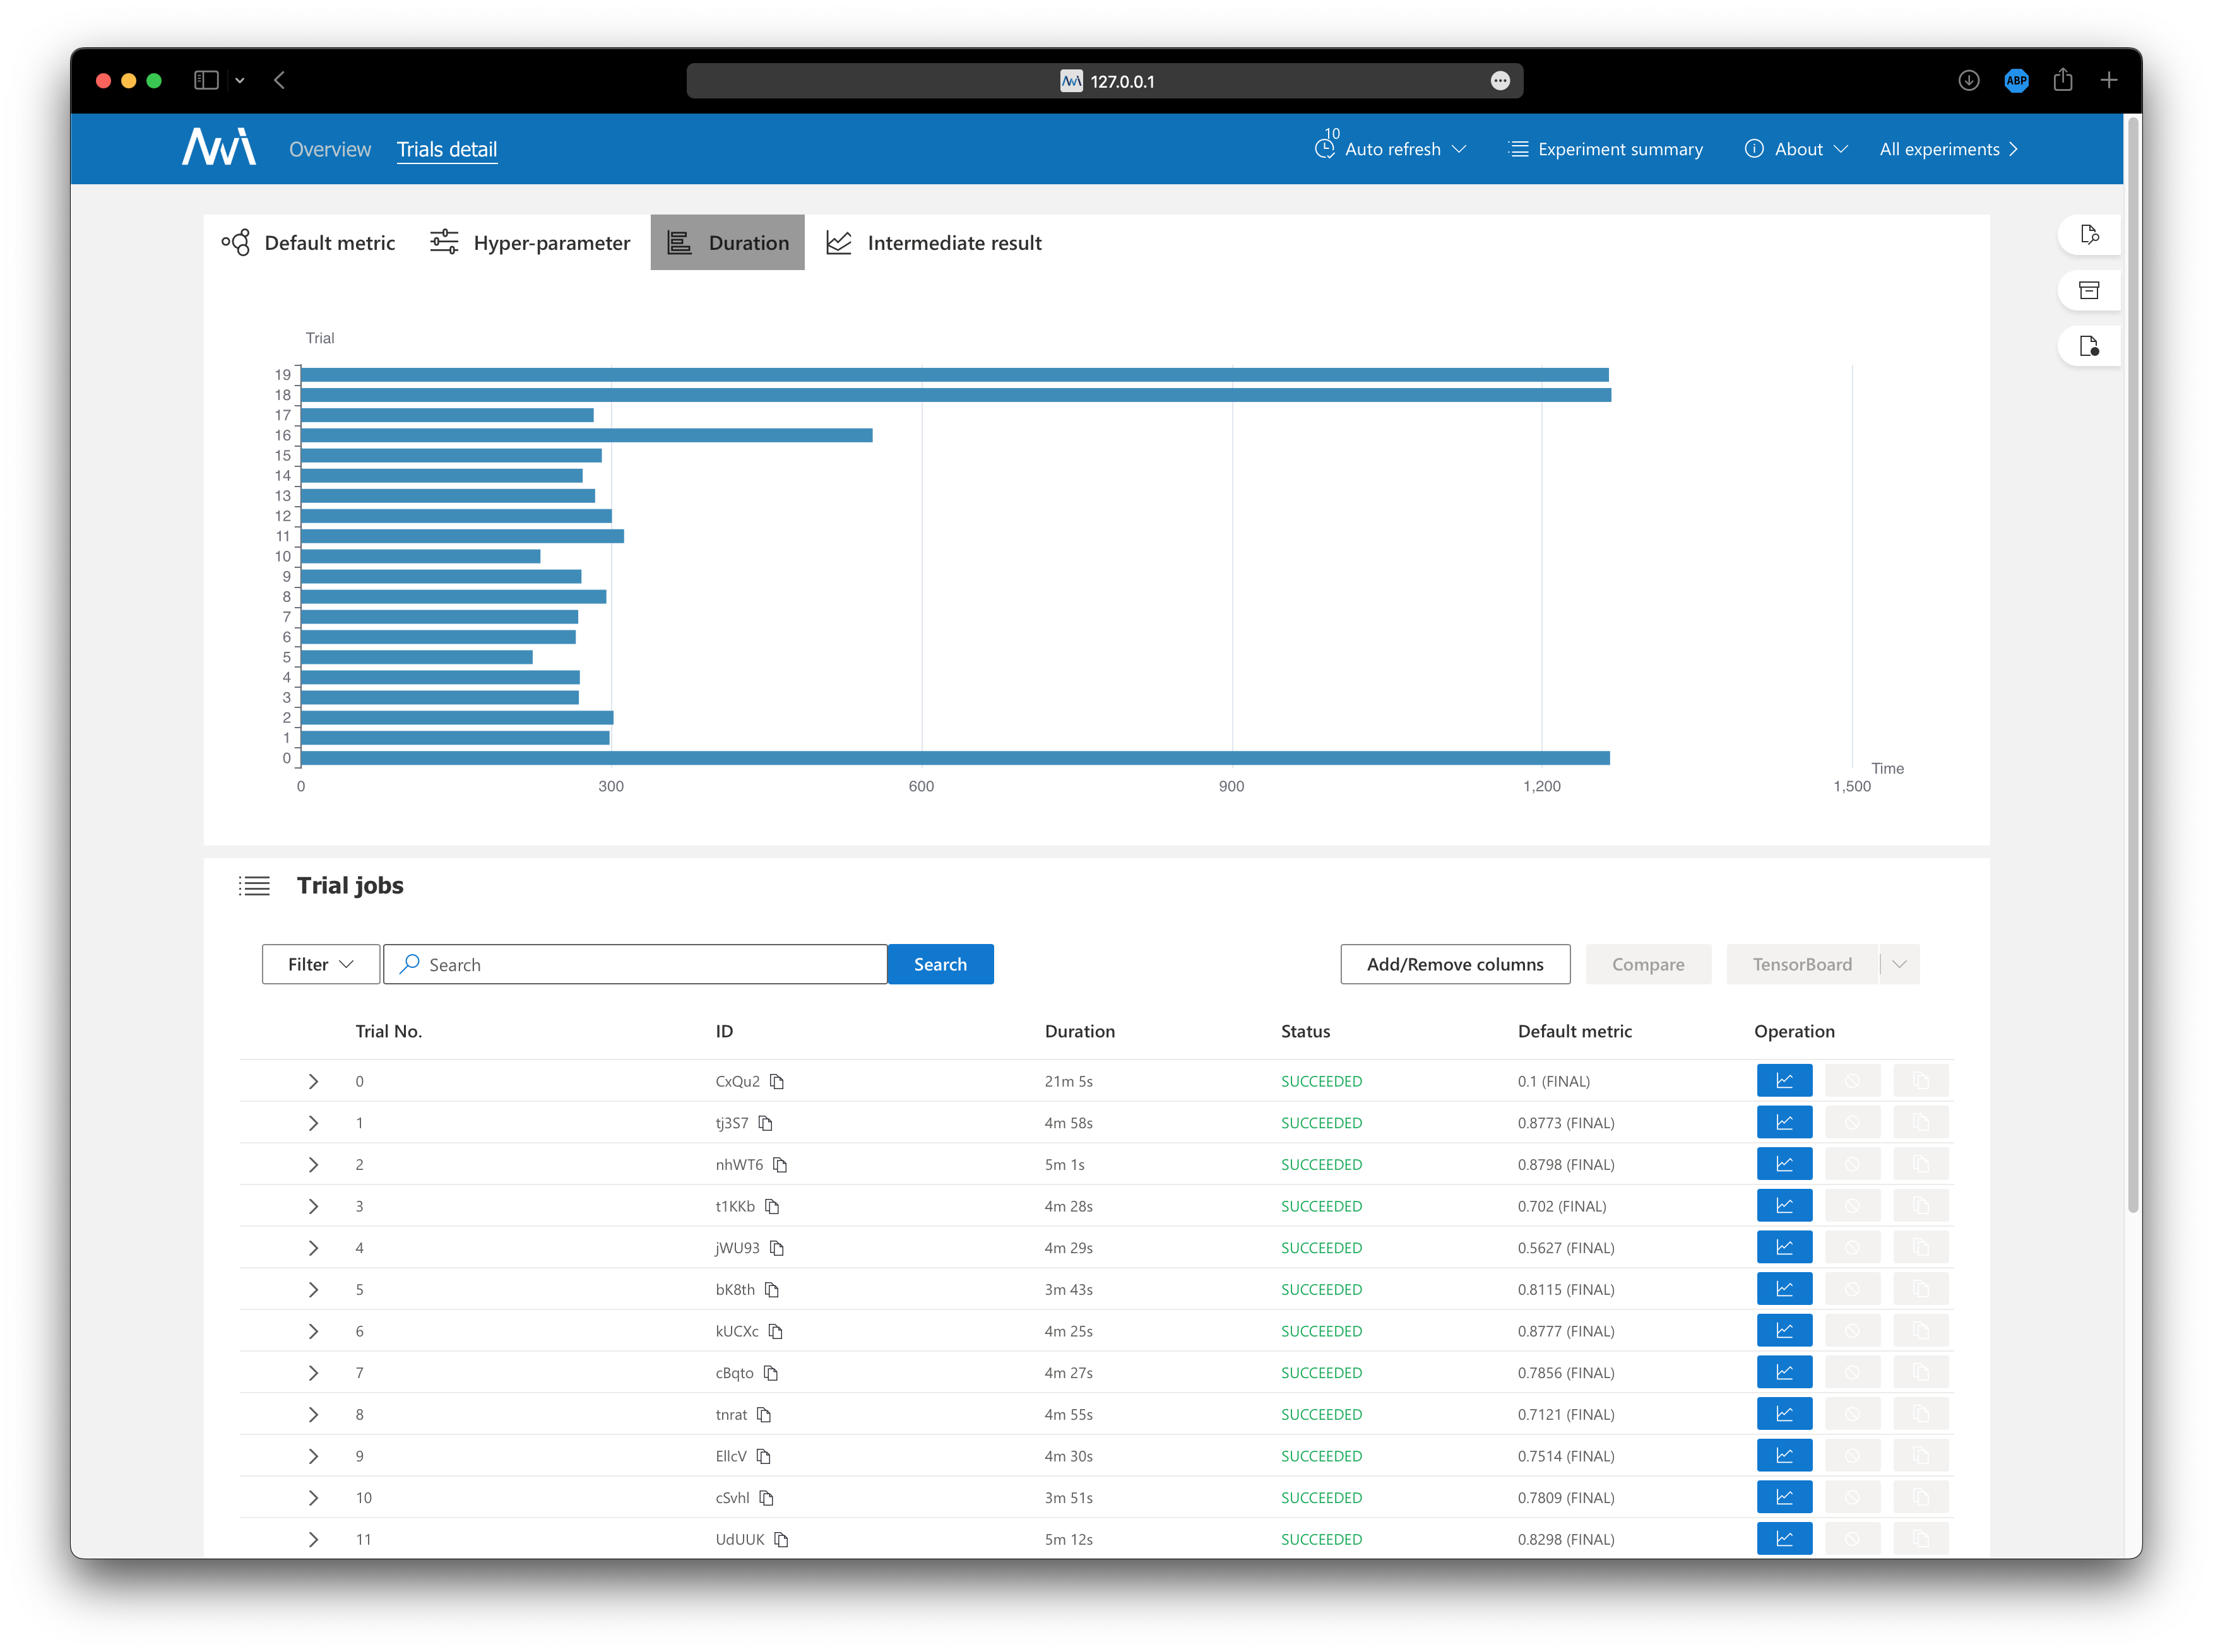
\includegraphics[width=3.5in]{../proj3/figures/mlp_evolution_batch_latency.png}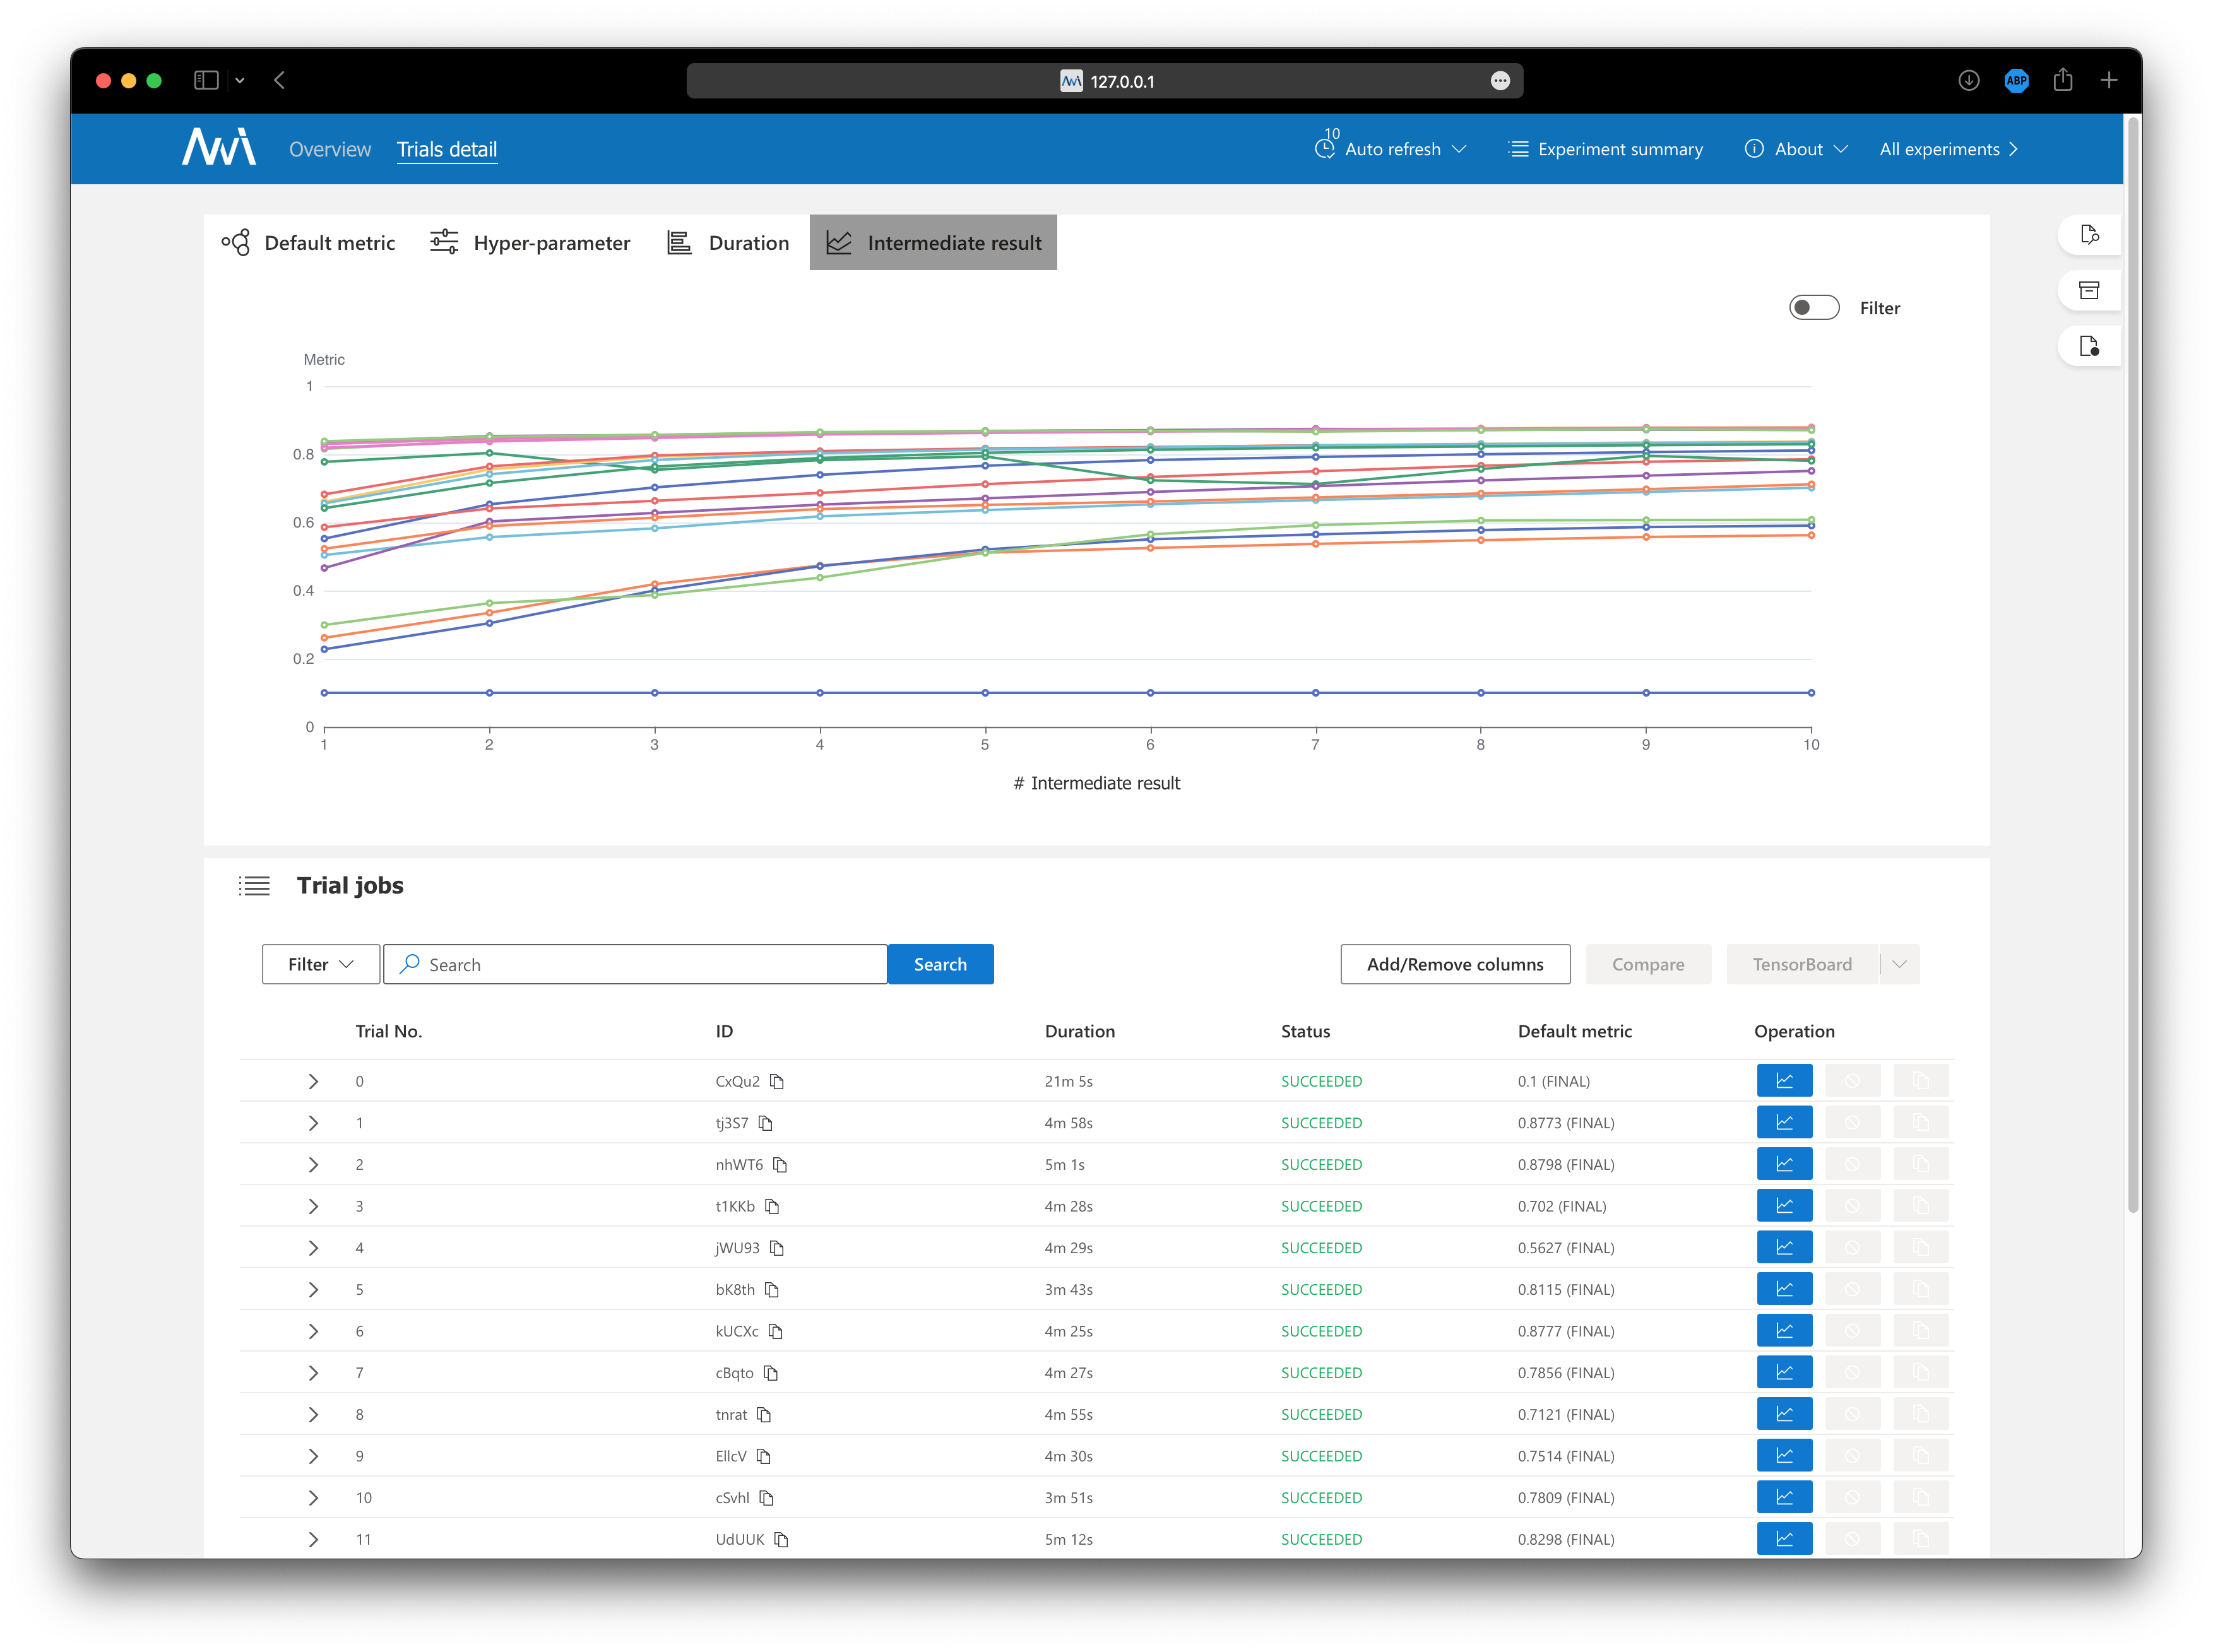
\includegraphics[width=3.5in]{../proj3/figures/mlp_evolution_batch_intermediate.png}}
    \caption{MLP with Evolution Tuner on Learning Rate, Momentum, Feature Size, and Batch Size}
    \label{fig:mlp-evolution-batch}
\end{figure}
\begin{figure}
    \centerline{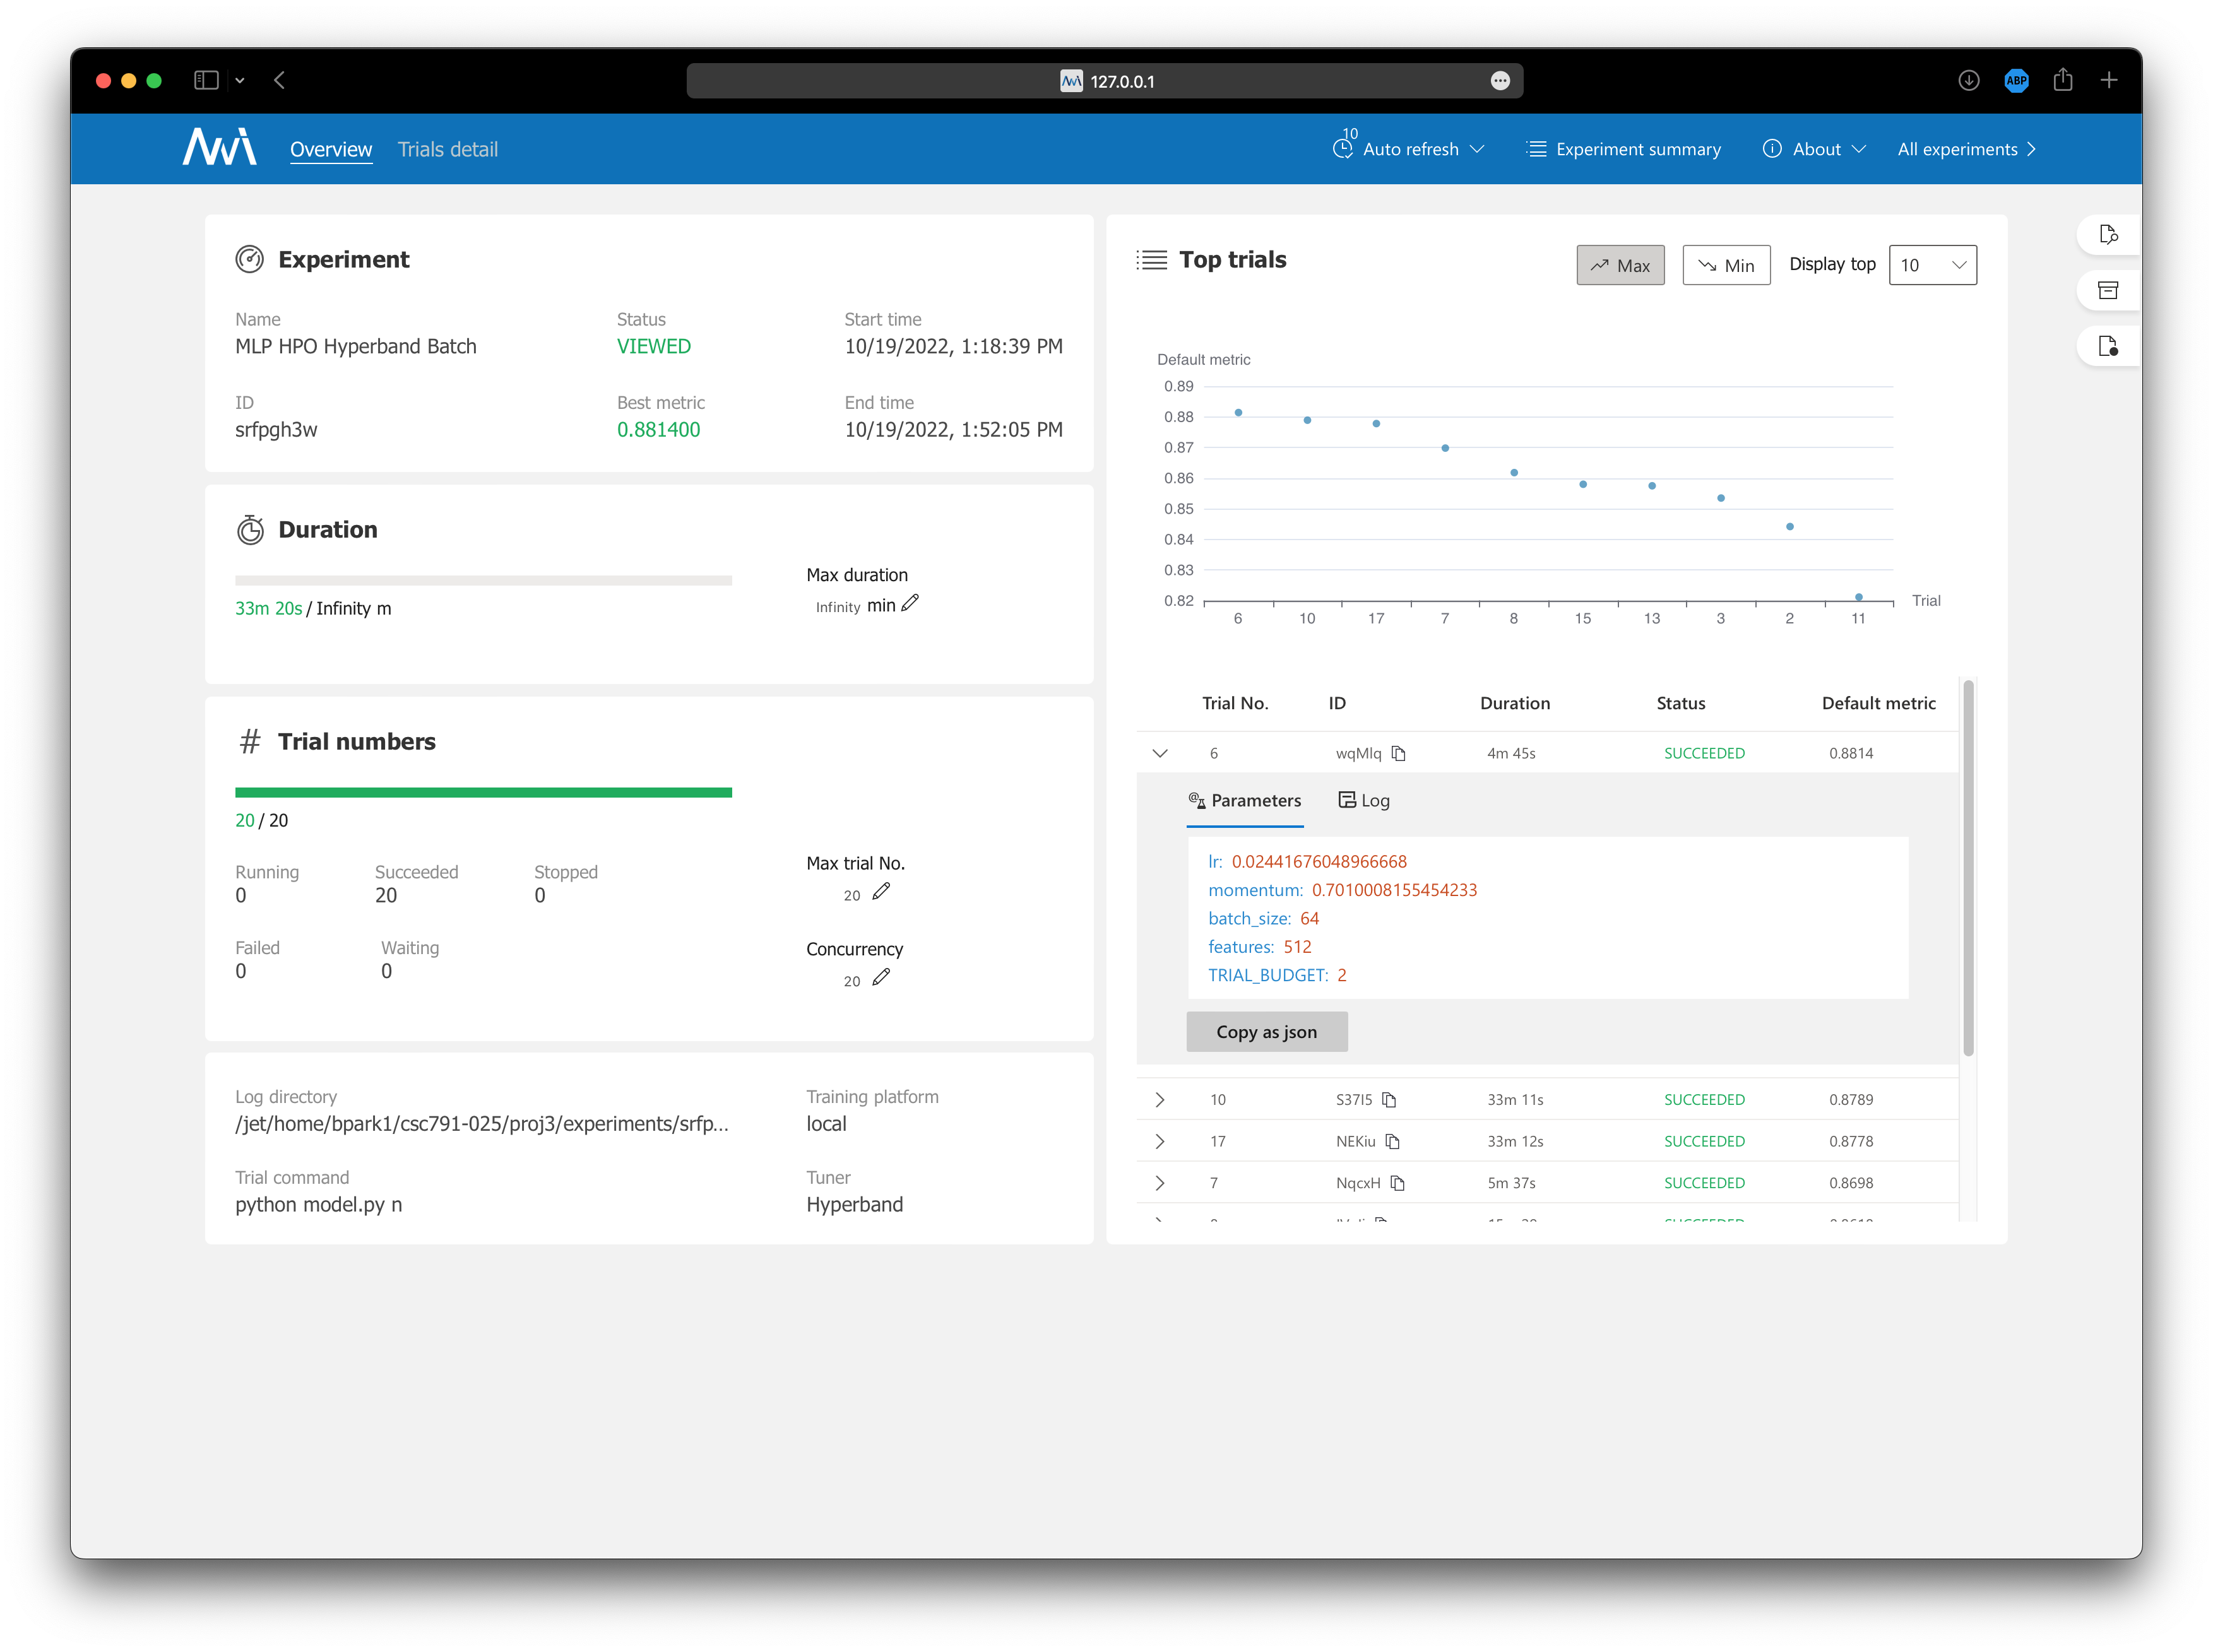
\includegraphics[width=3.5in]{../proj3/figures/mlp_hyperband_batch_overview.png}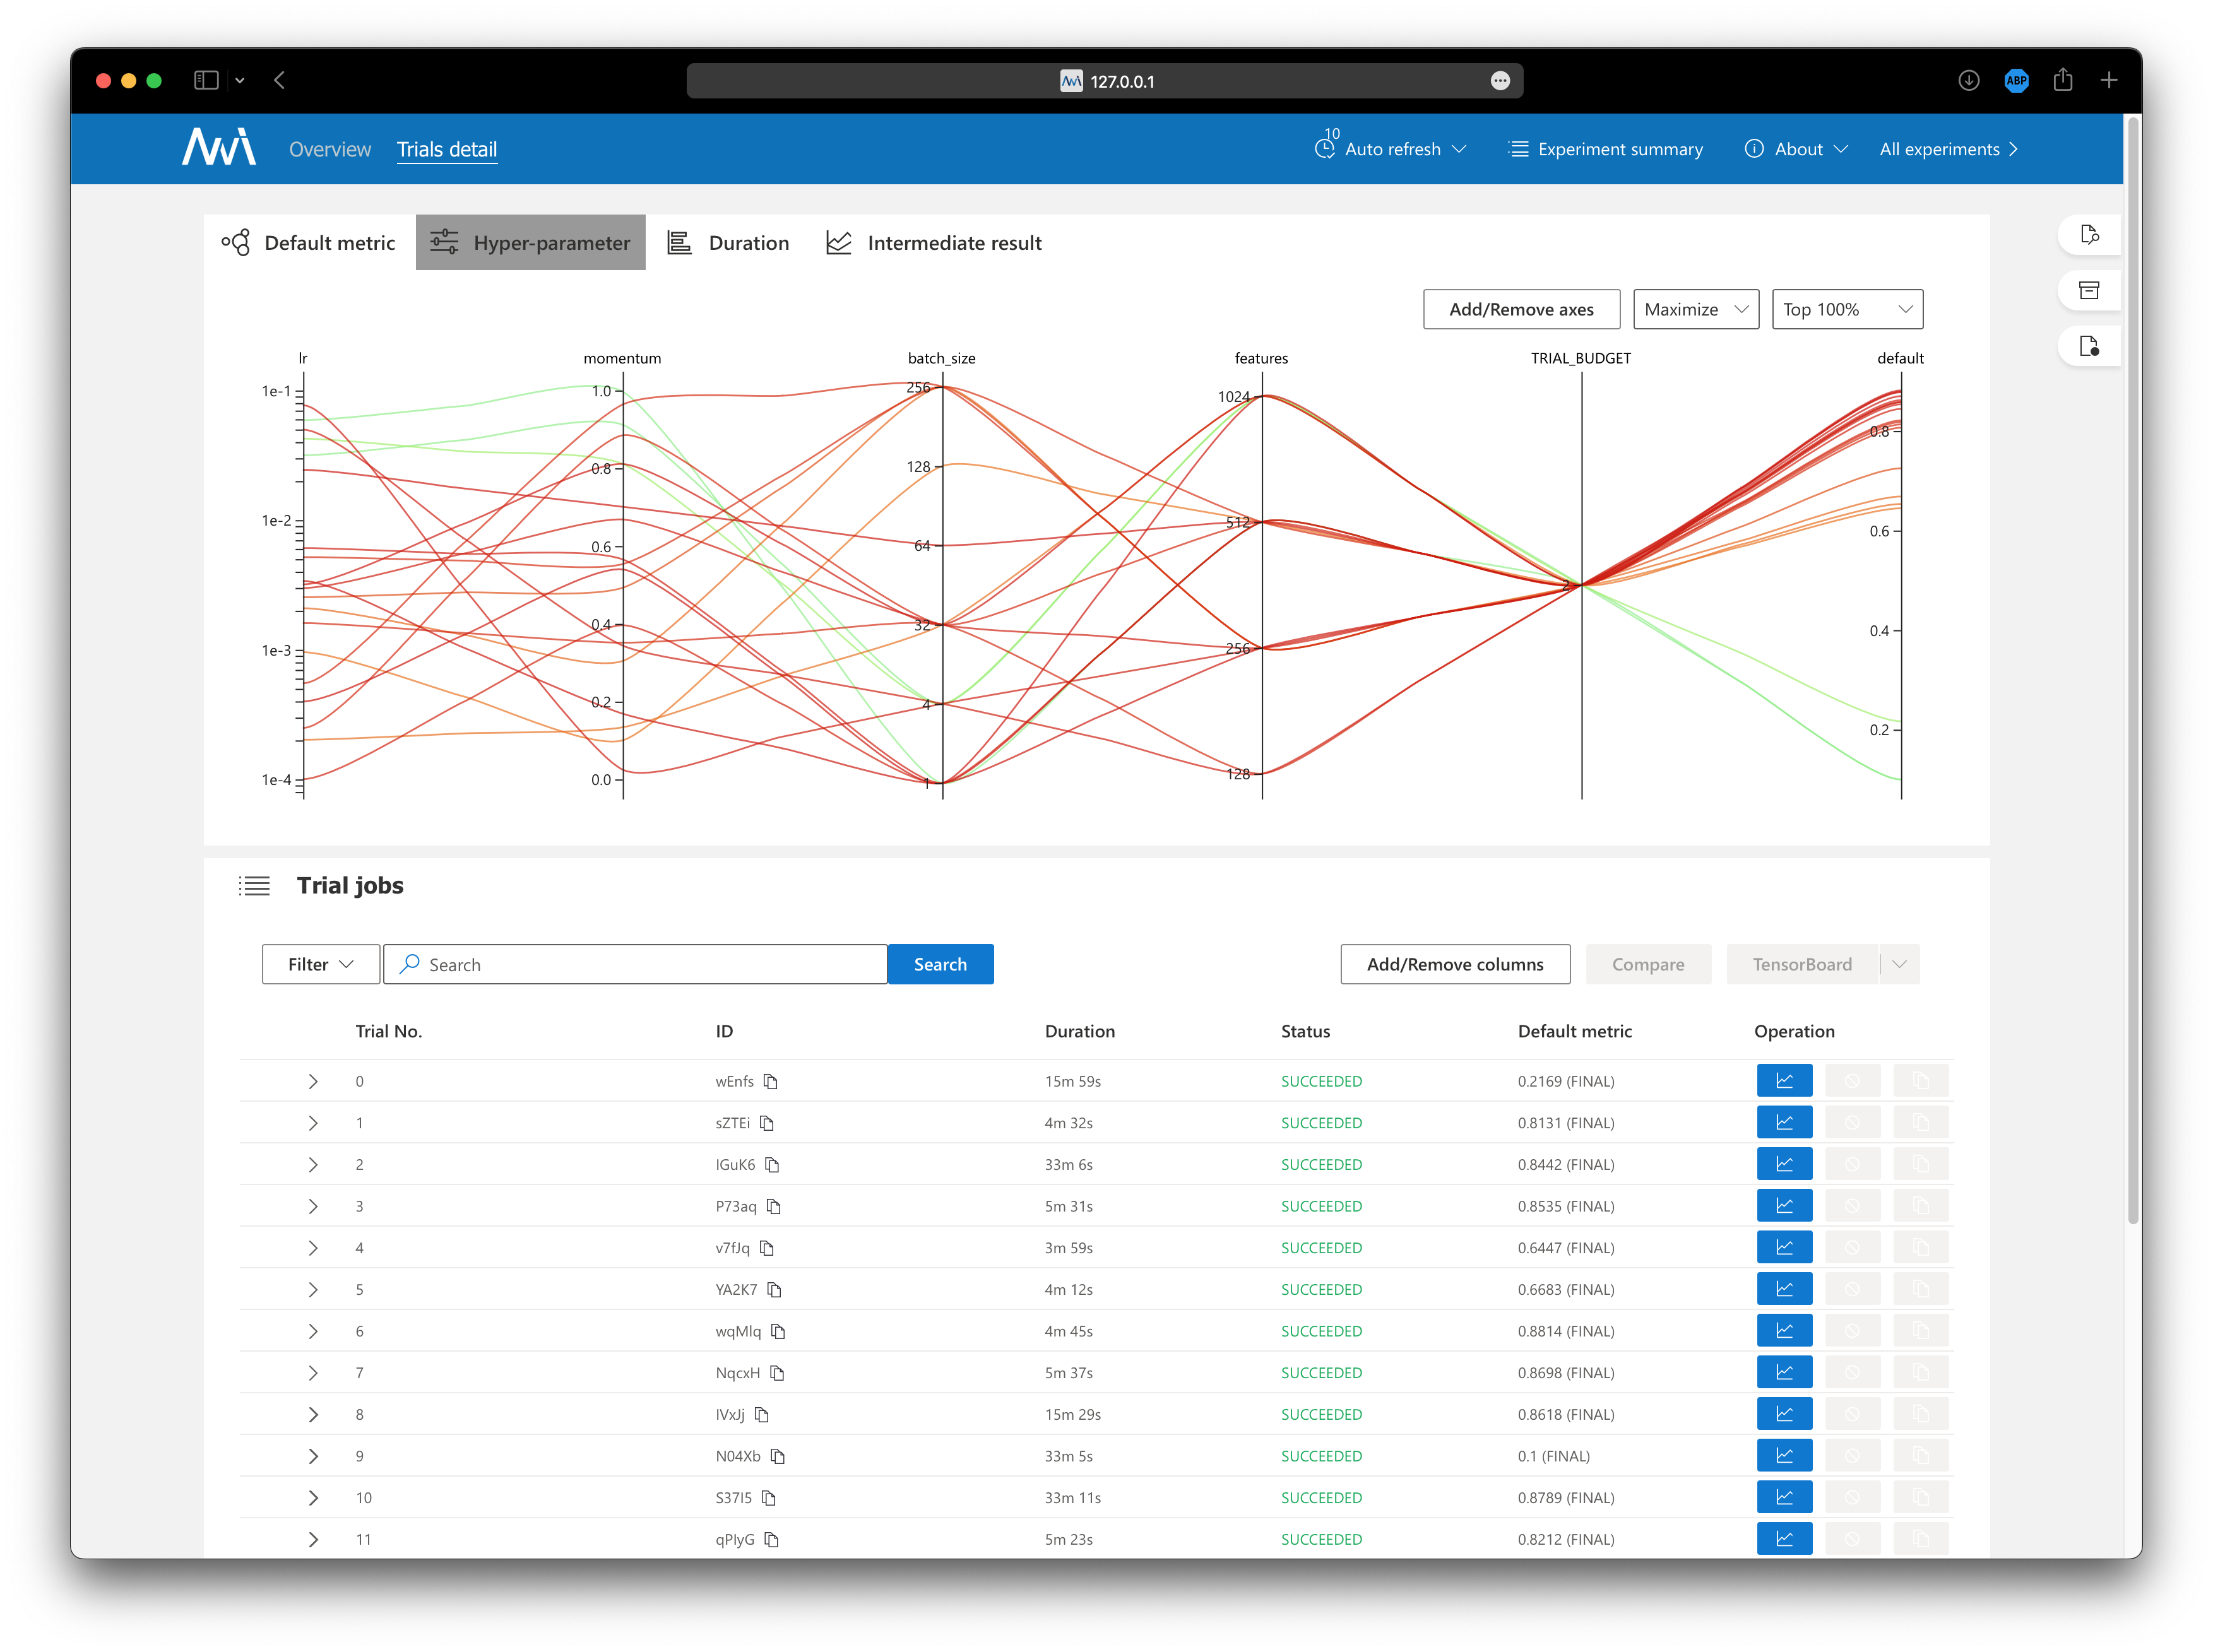
\includegraphics[width=3.5in]{../proj3/figures/mlp_hyperband_batch_hyperparameter.png}}
    \centerline{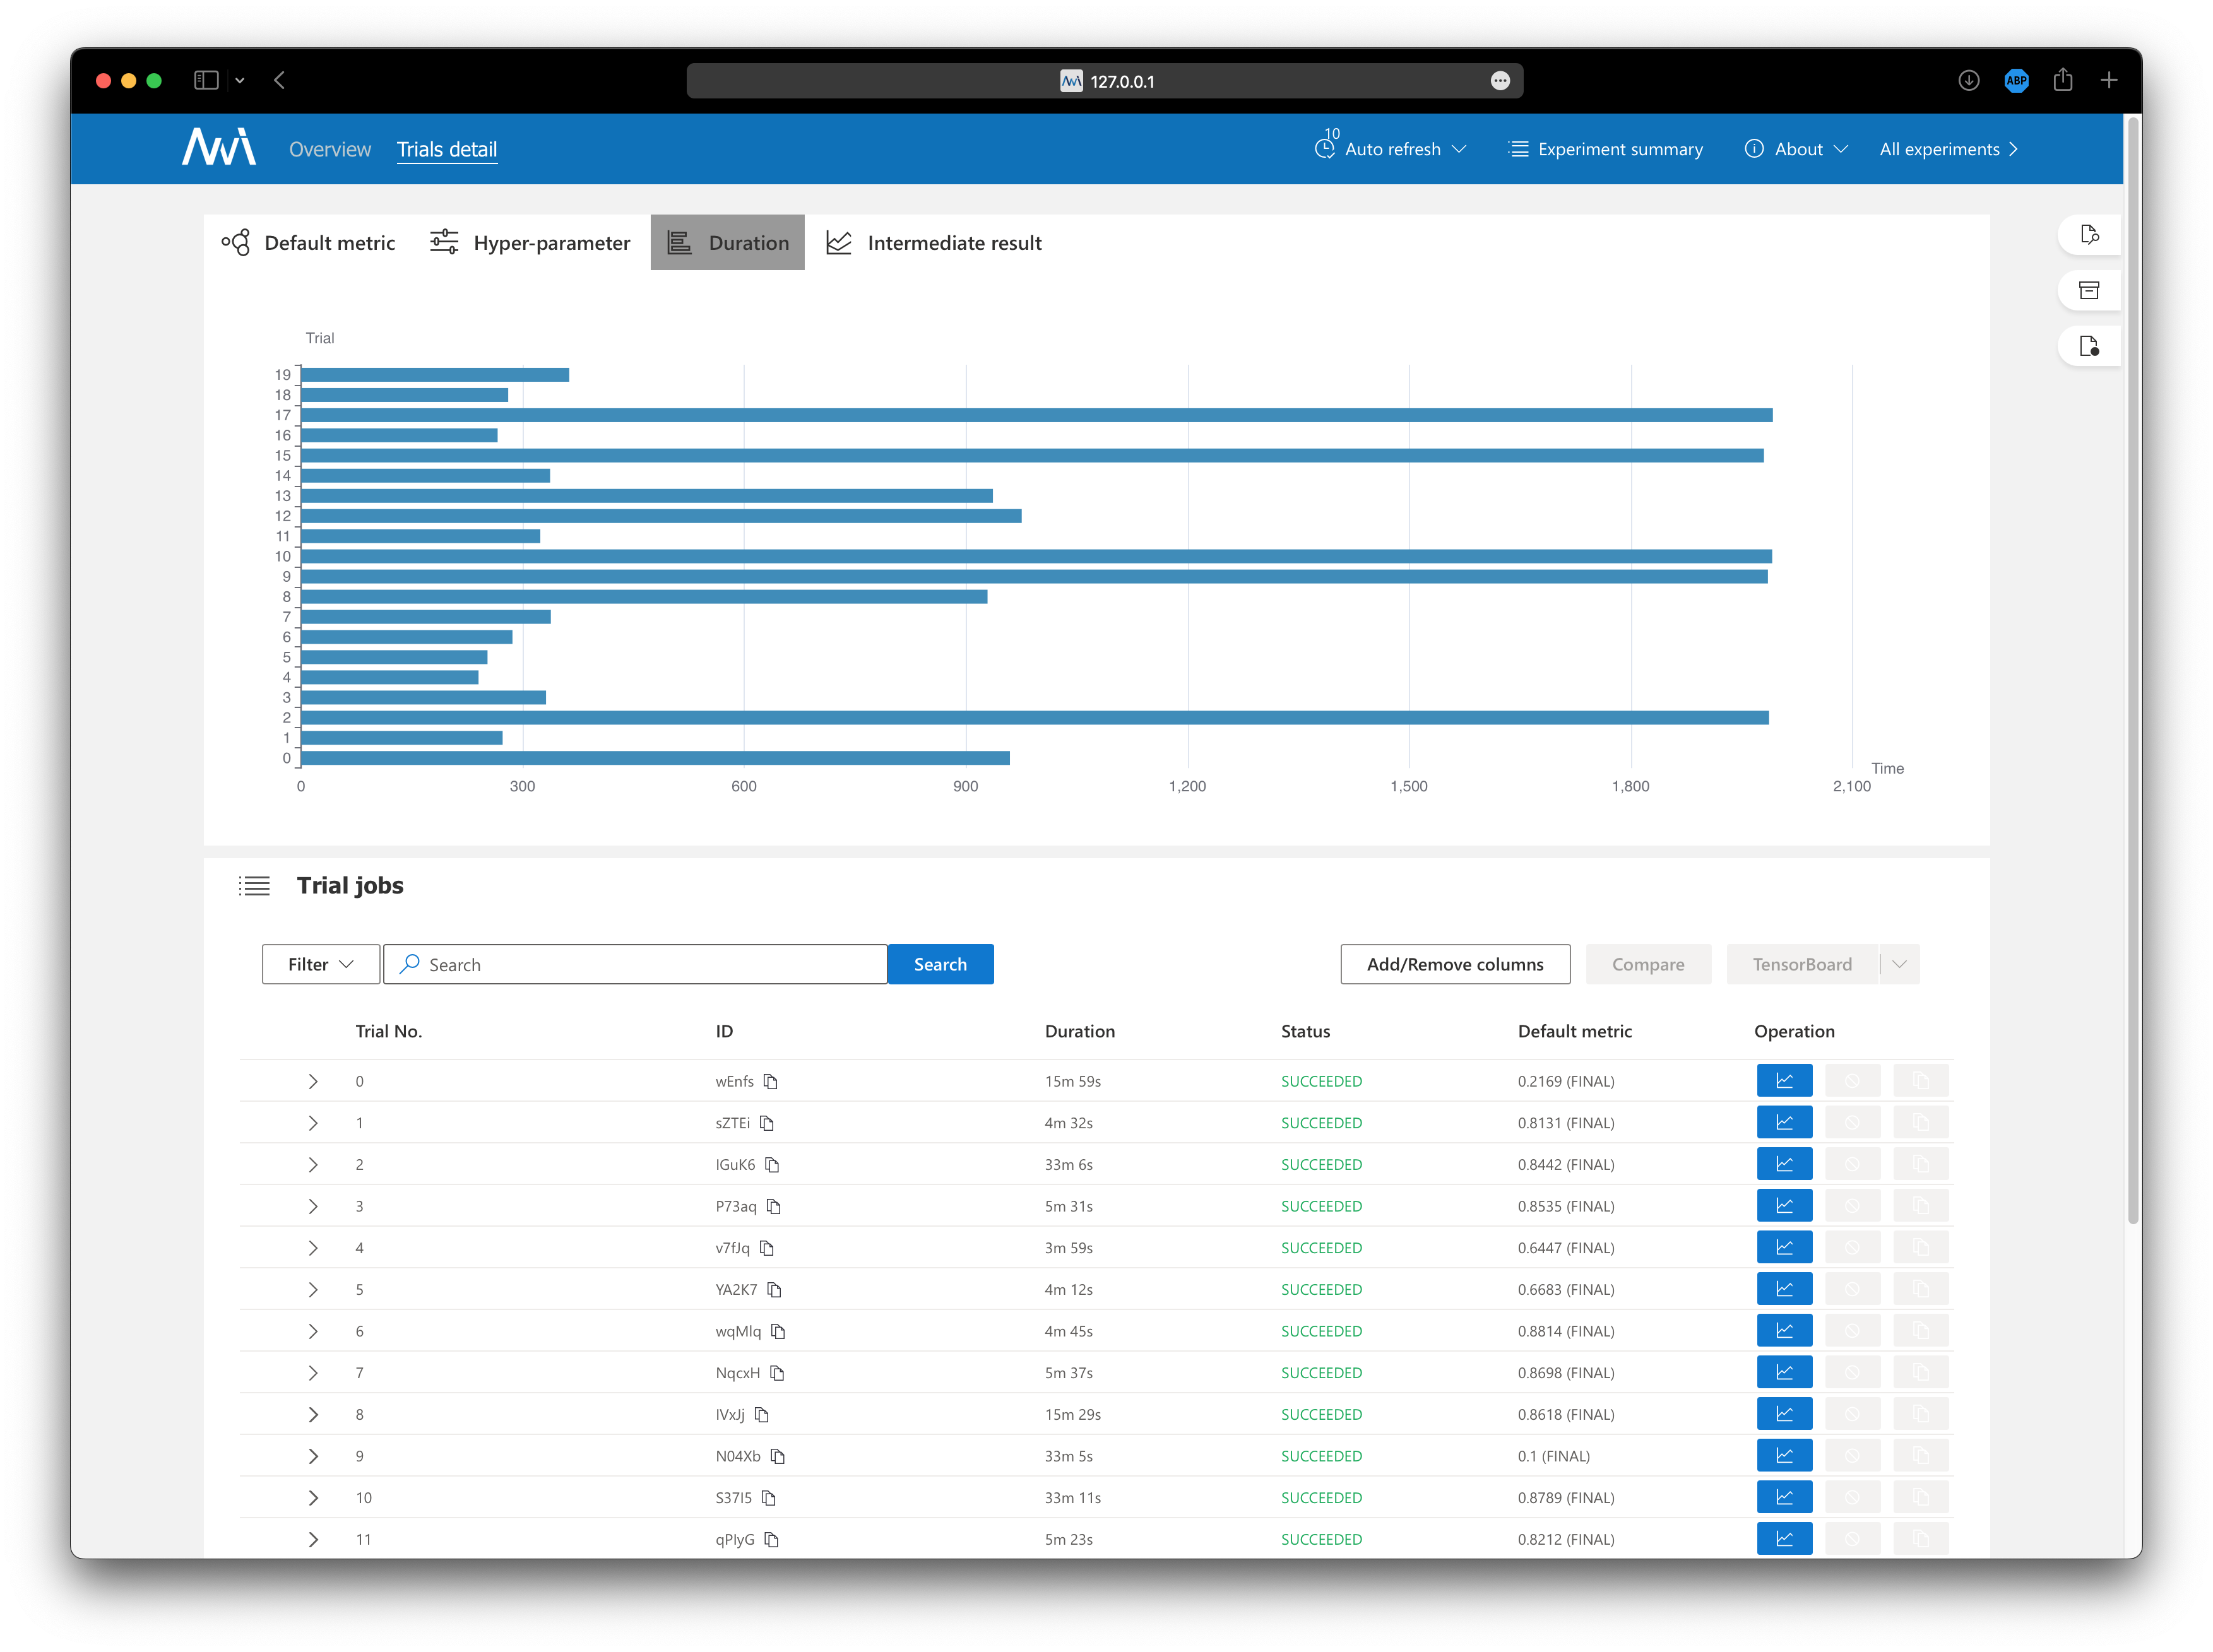
\includegraphics[width=3.5in]{../proj3/figures/mlp_hyperband_batch_latency.png}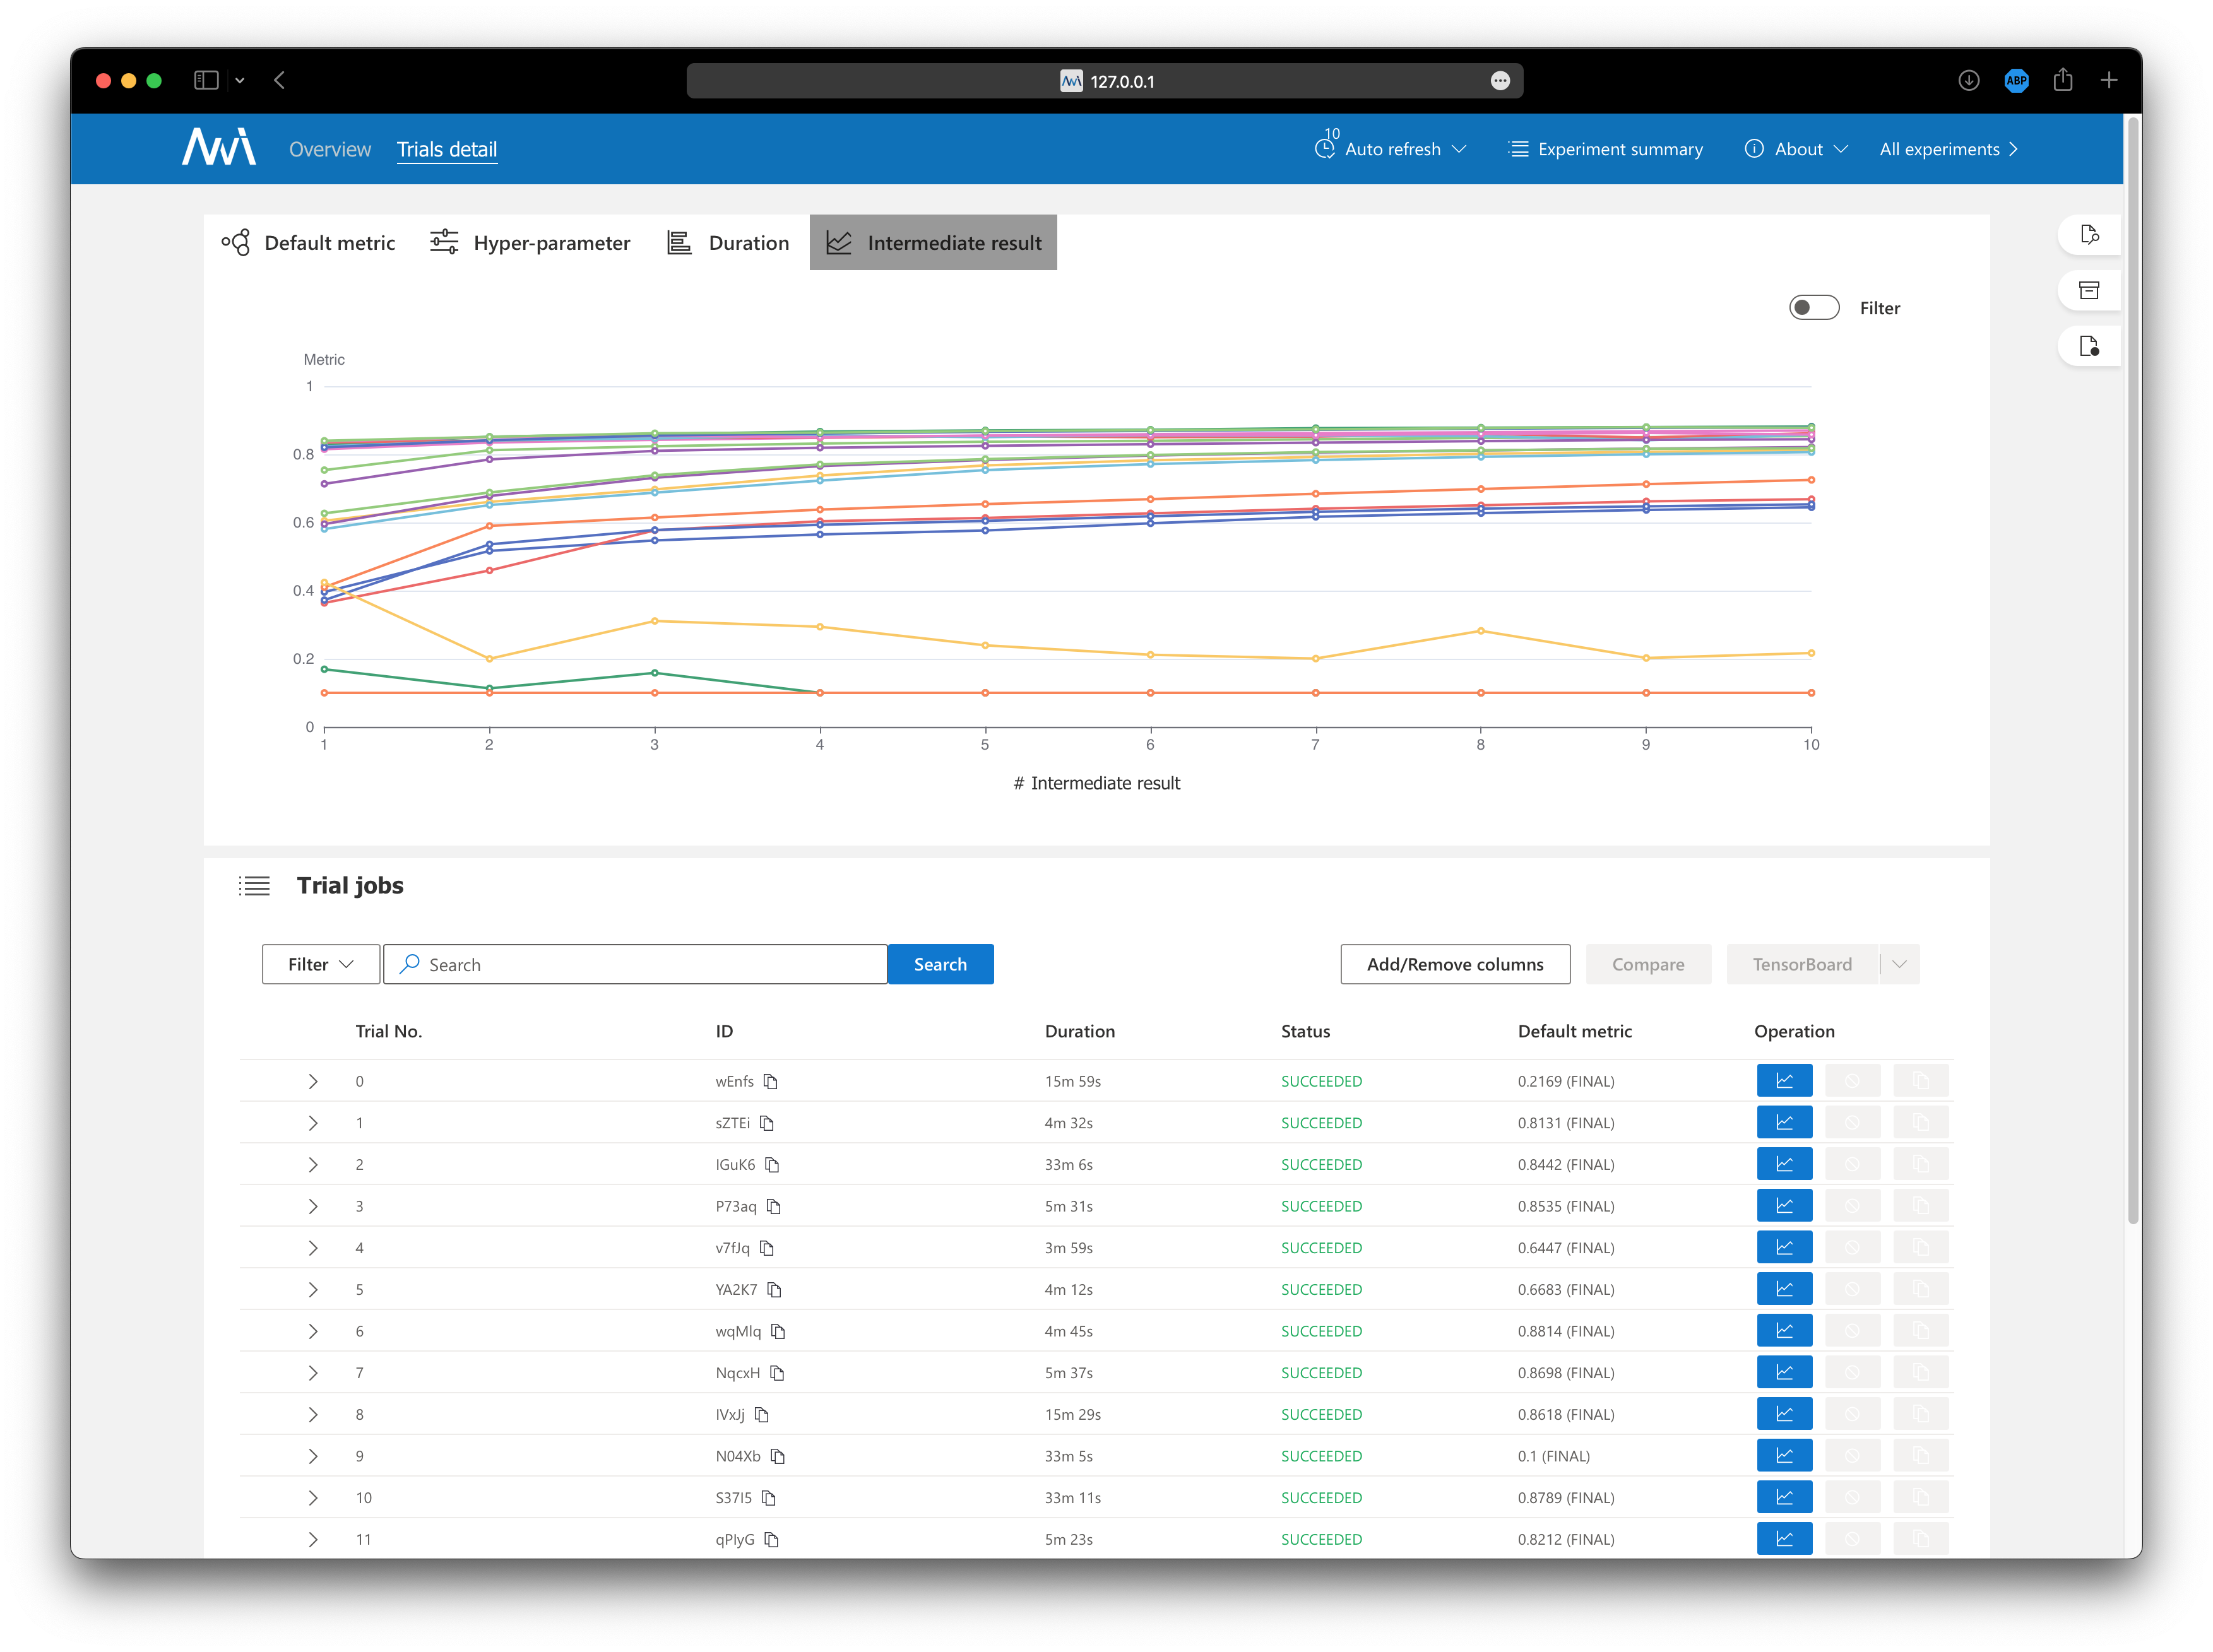
\includegraphics[width=3.5in]{../proj3/figures/mlp_hyperband_batch_intermediate.png}}
    \caption{MLP with Hyperband Tuner on Learning Rate, Momentum, Feature Size, and Batch Size}
    \label{fig:mlp-hyperband-batch}
\end{figure}
\begin{figure}
    \centerline{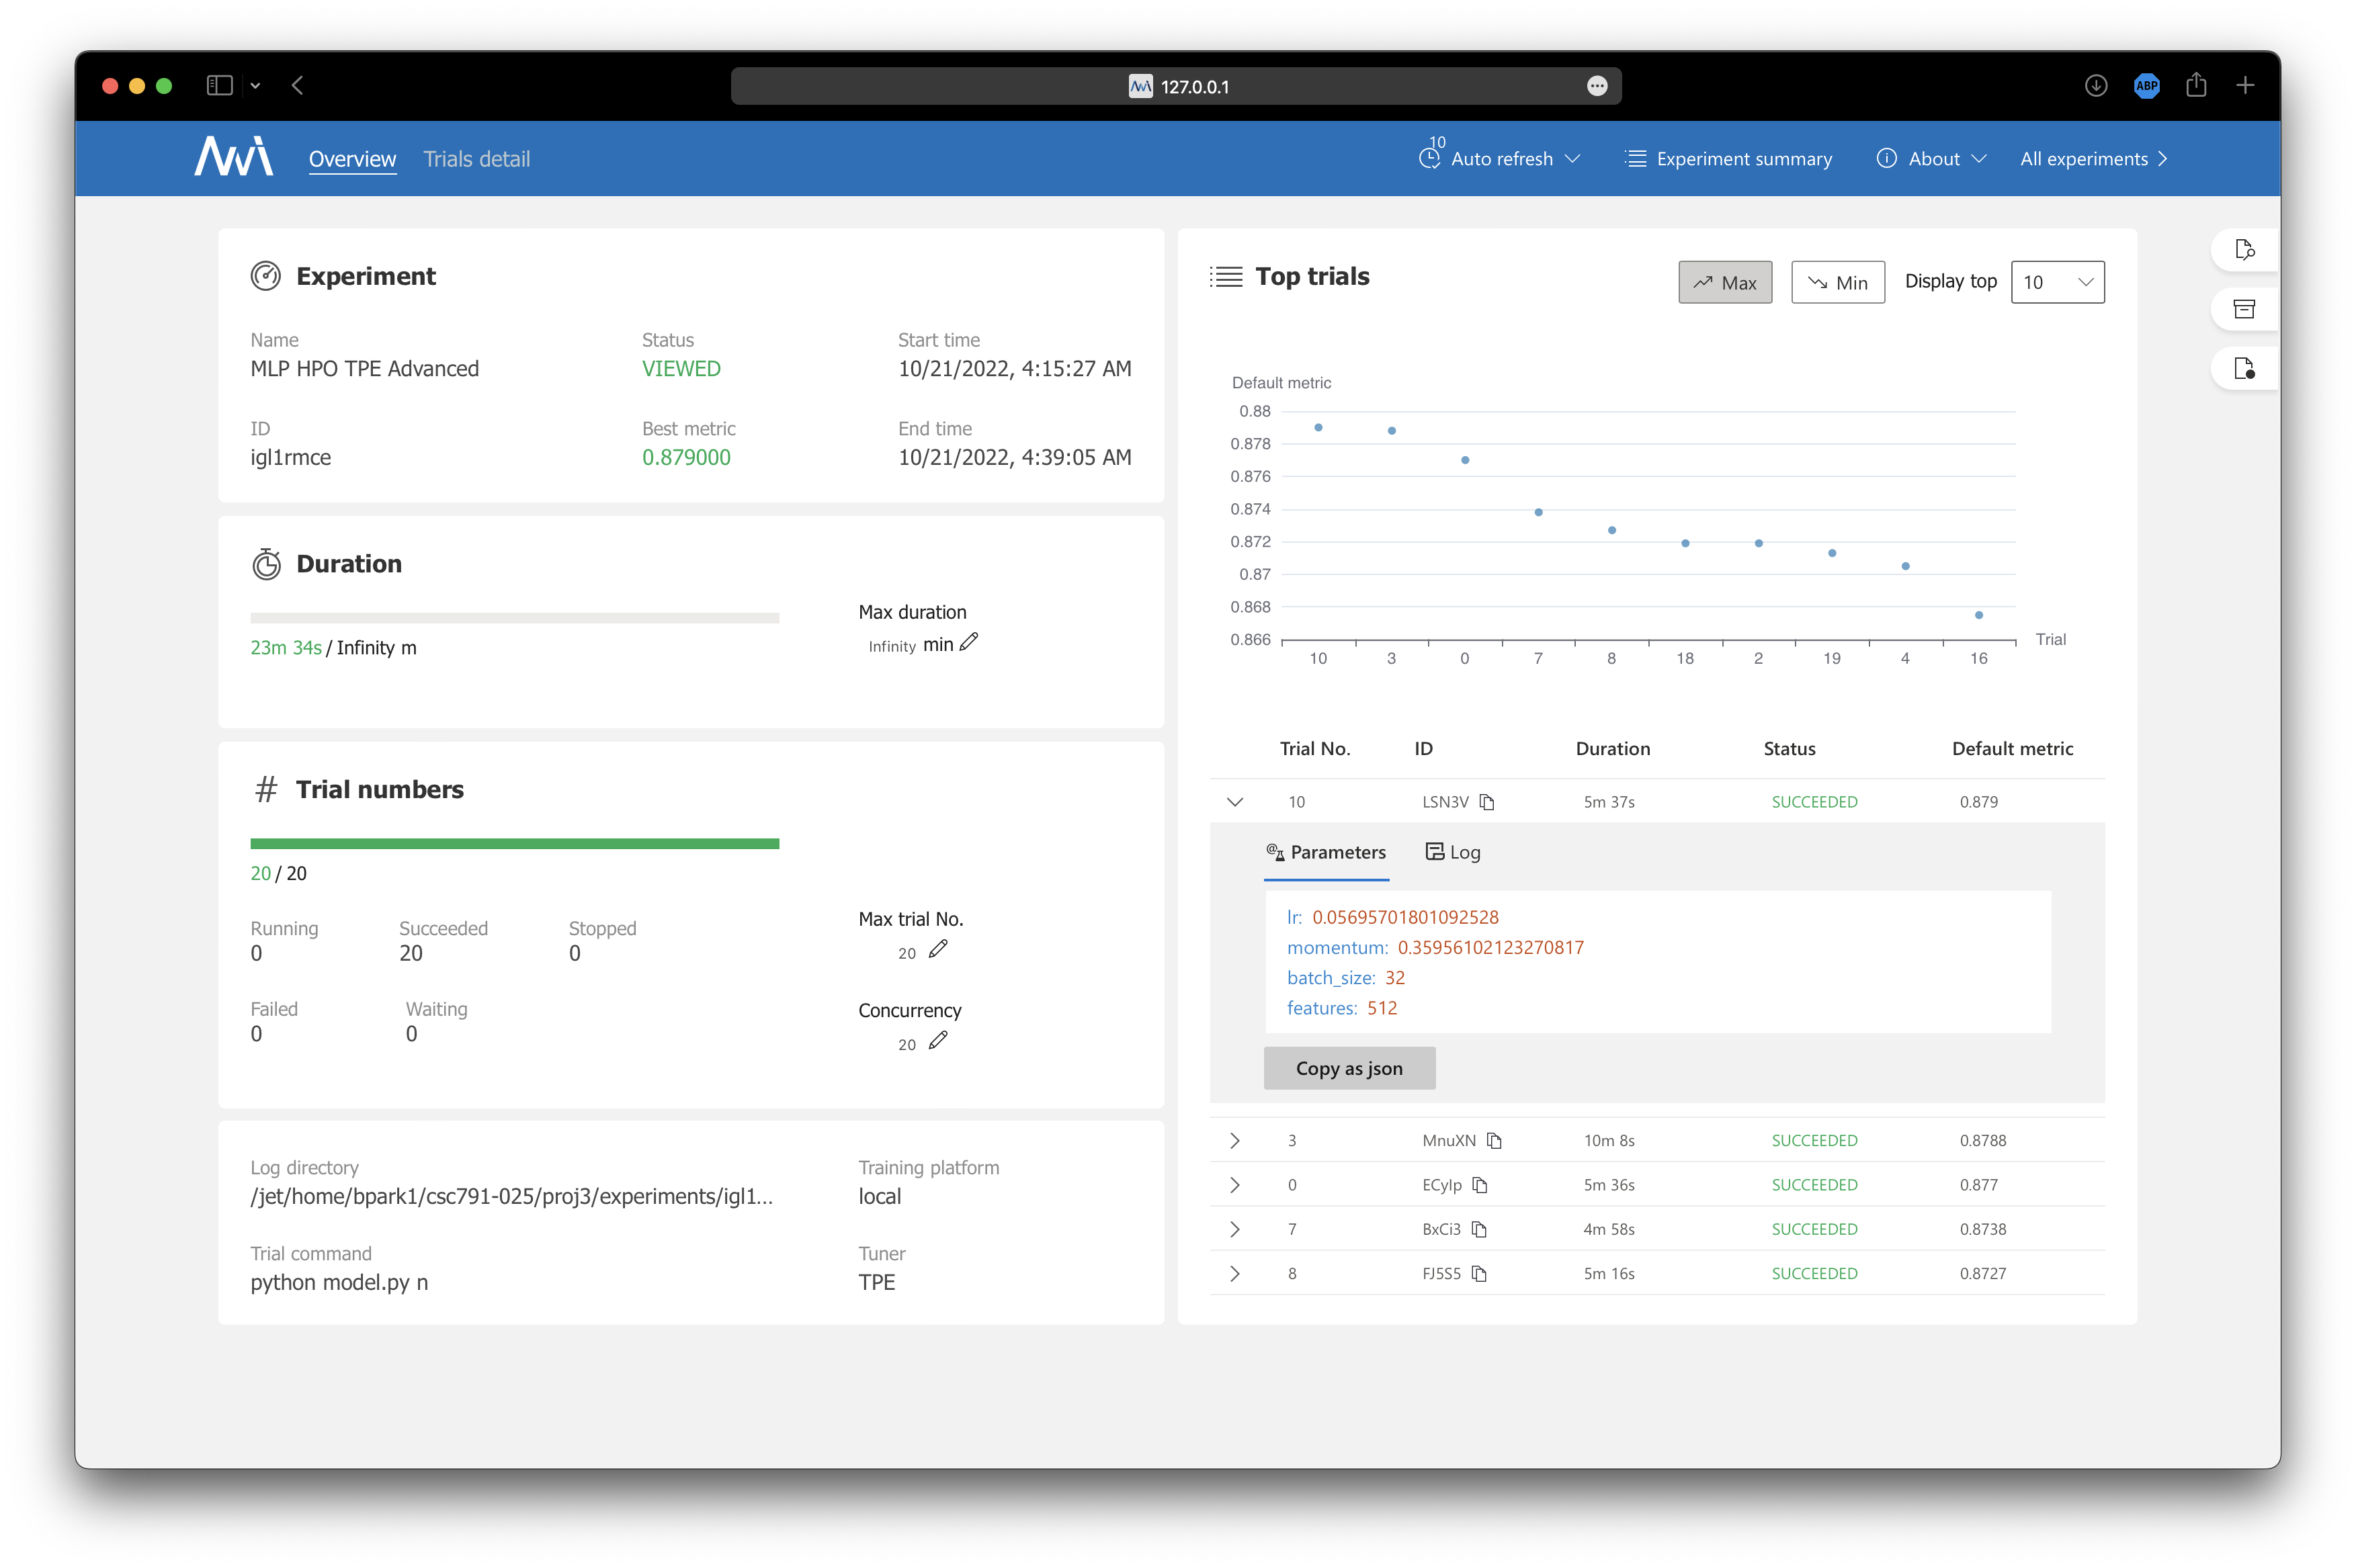
\includegraphics[width=3.5in]{../proj3/figures/mlp_tpe_batch_advanced_overview.png}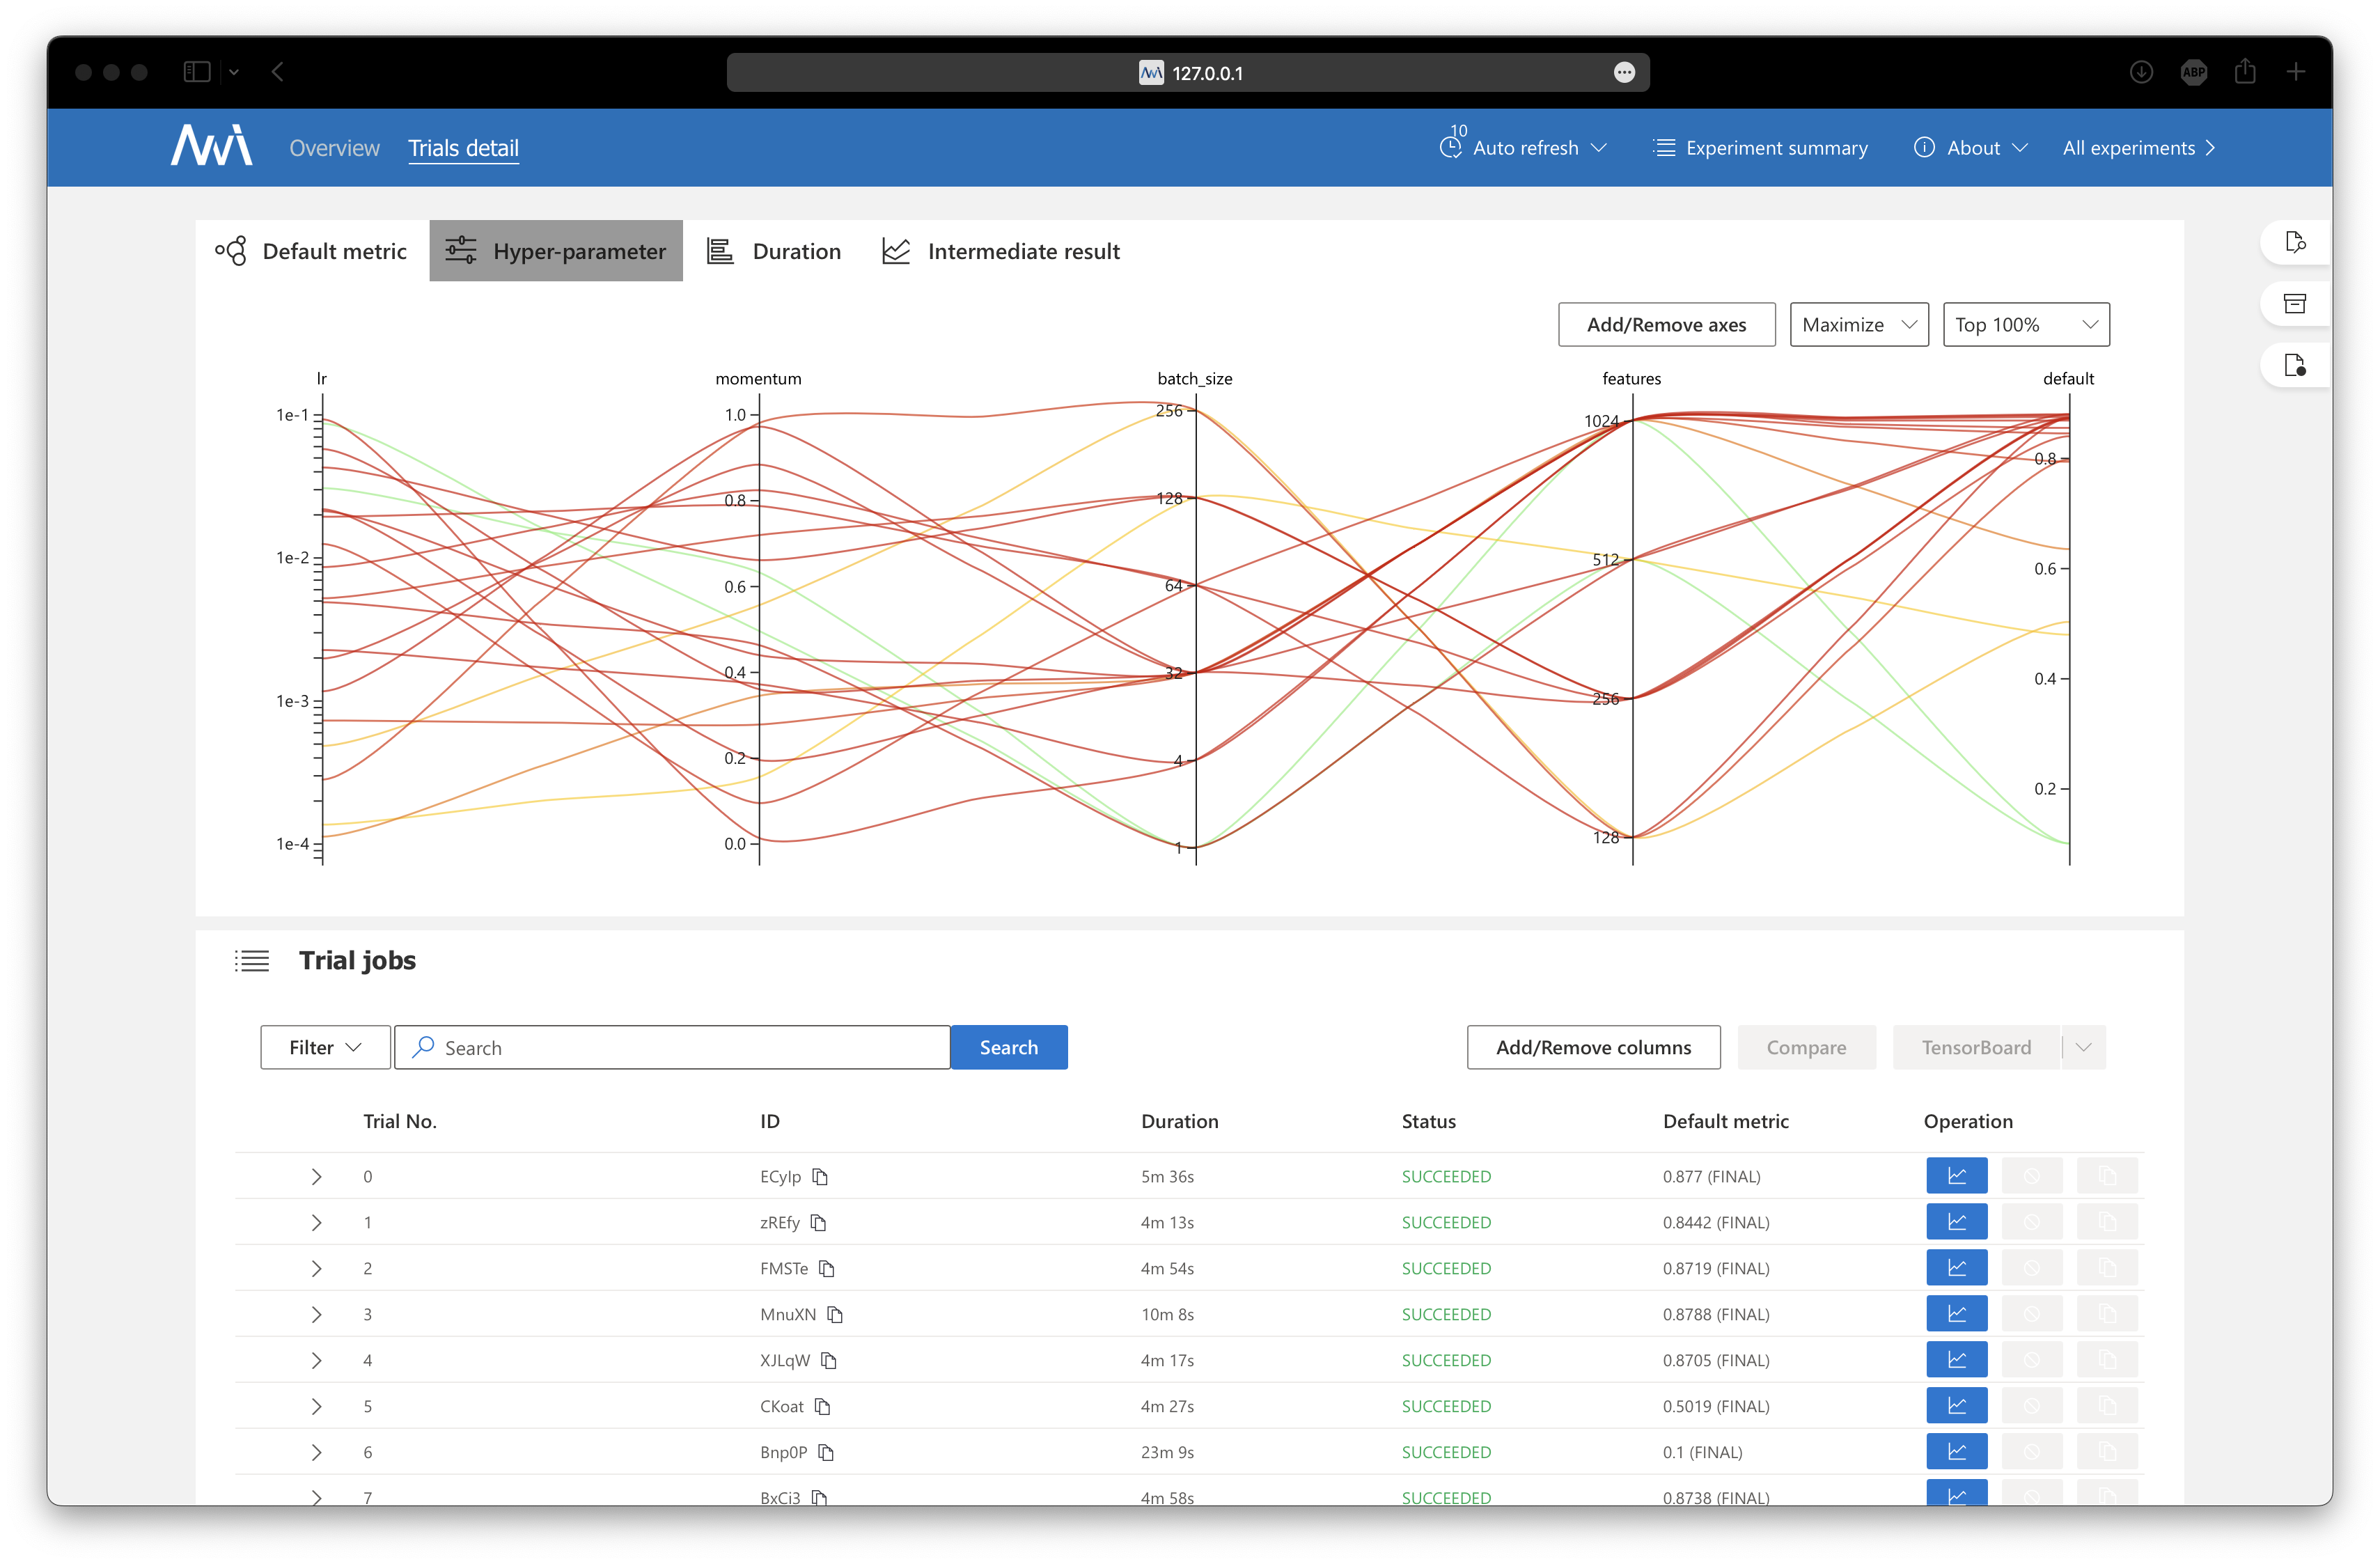
\includegraphics[width=3.5in]{../proj3/figures/mlp_tpe_batch_advanced_hyperparameter.png}}
    \centerline{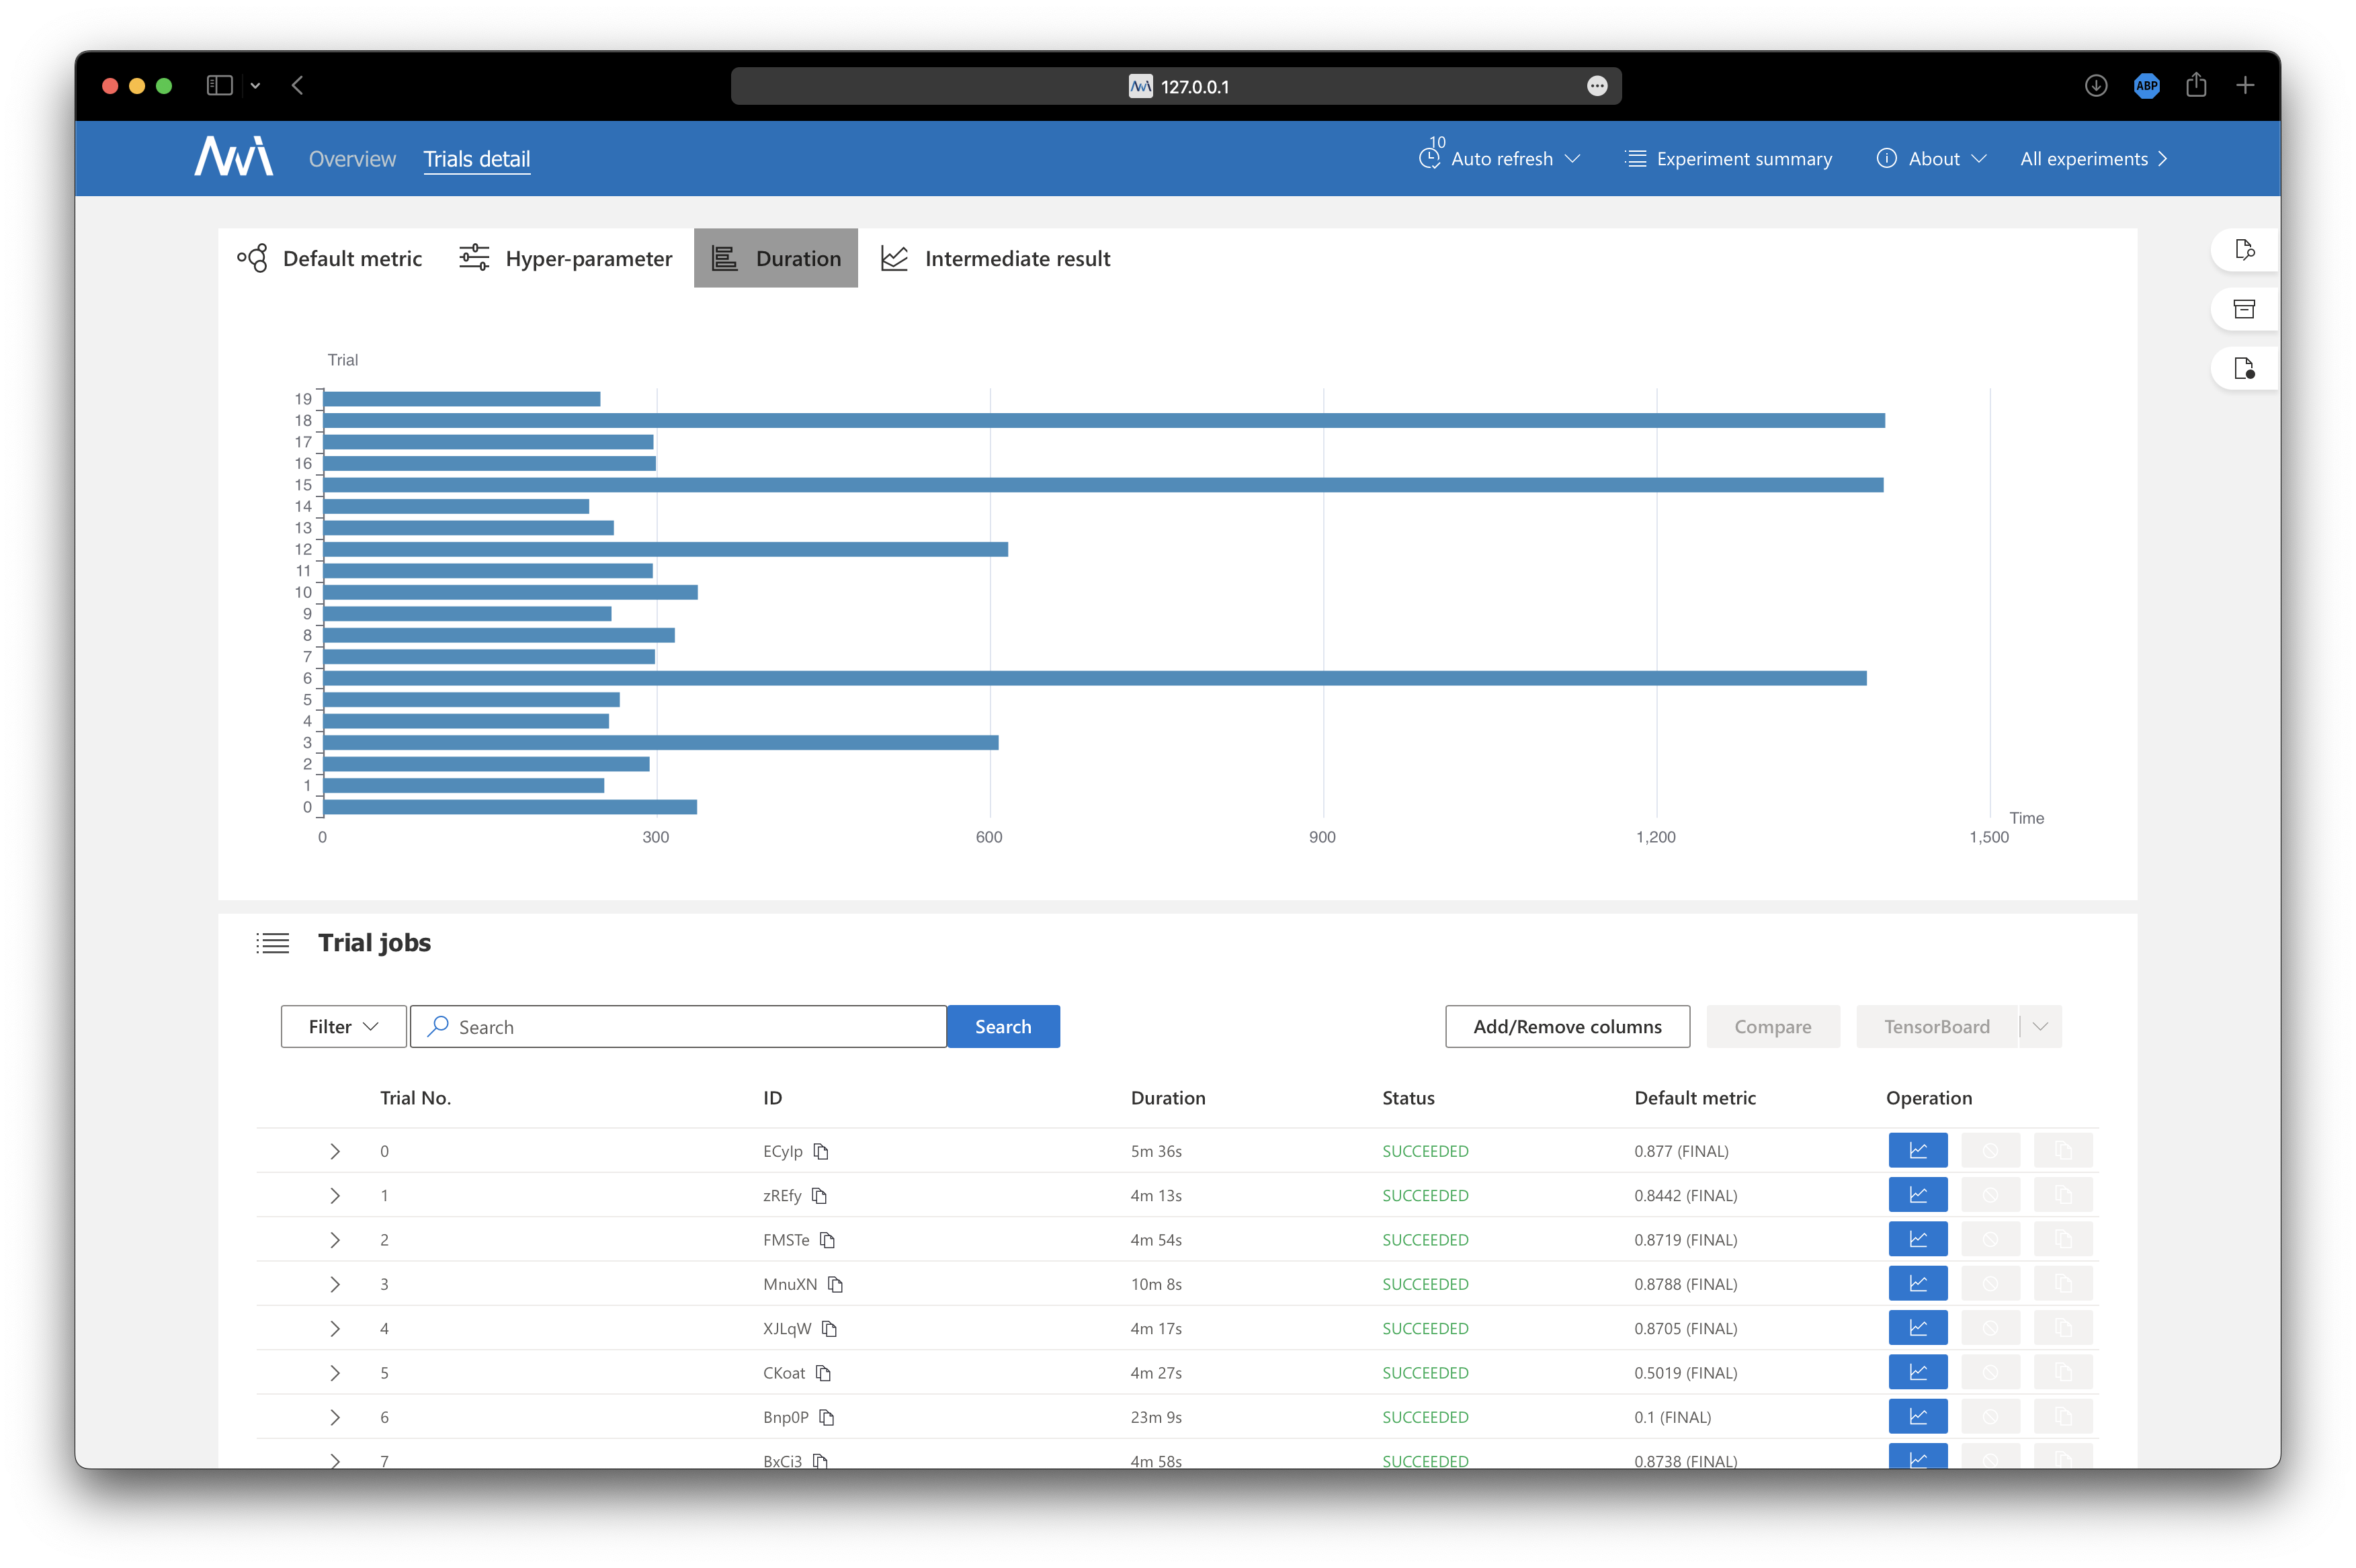
\includegraphics[width=3.5in]{../proj3/figures/mlp_tpe_batch_advanced_latency.png}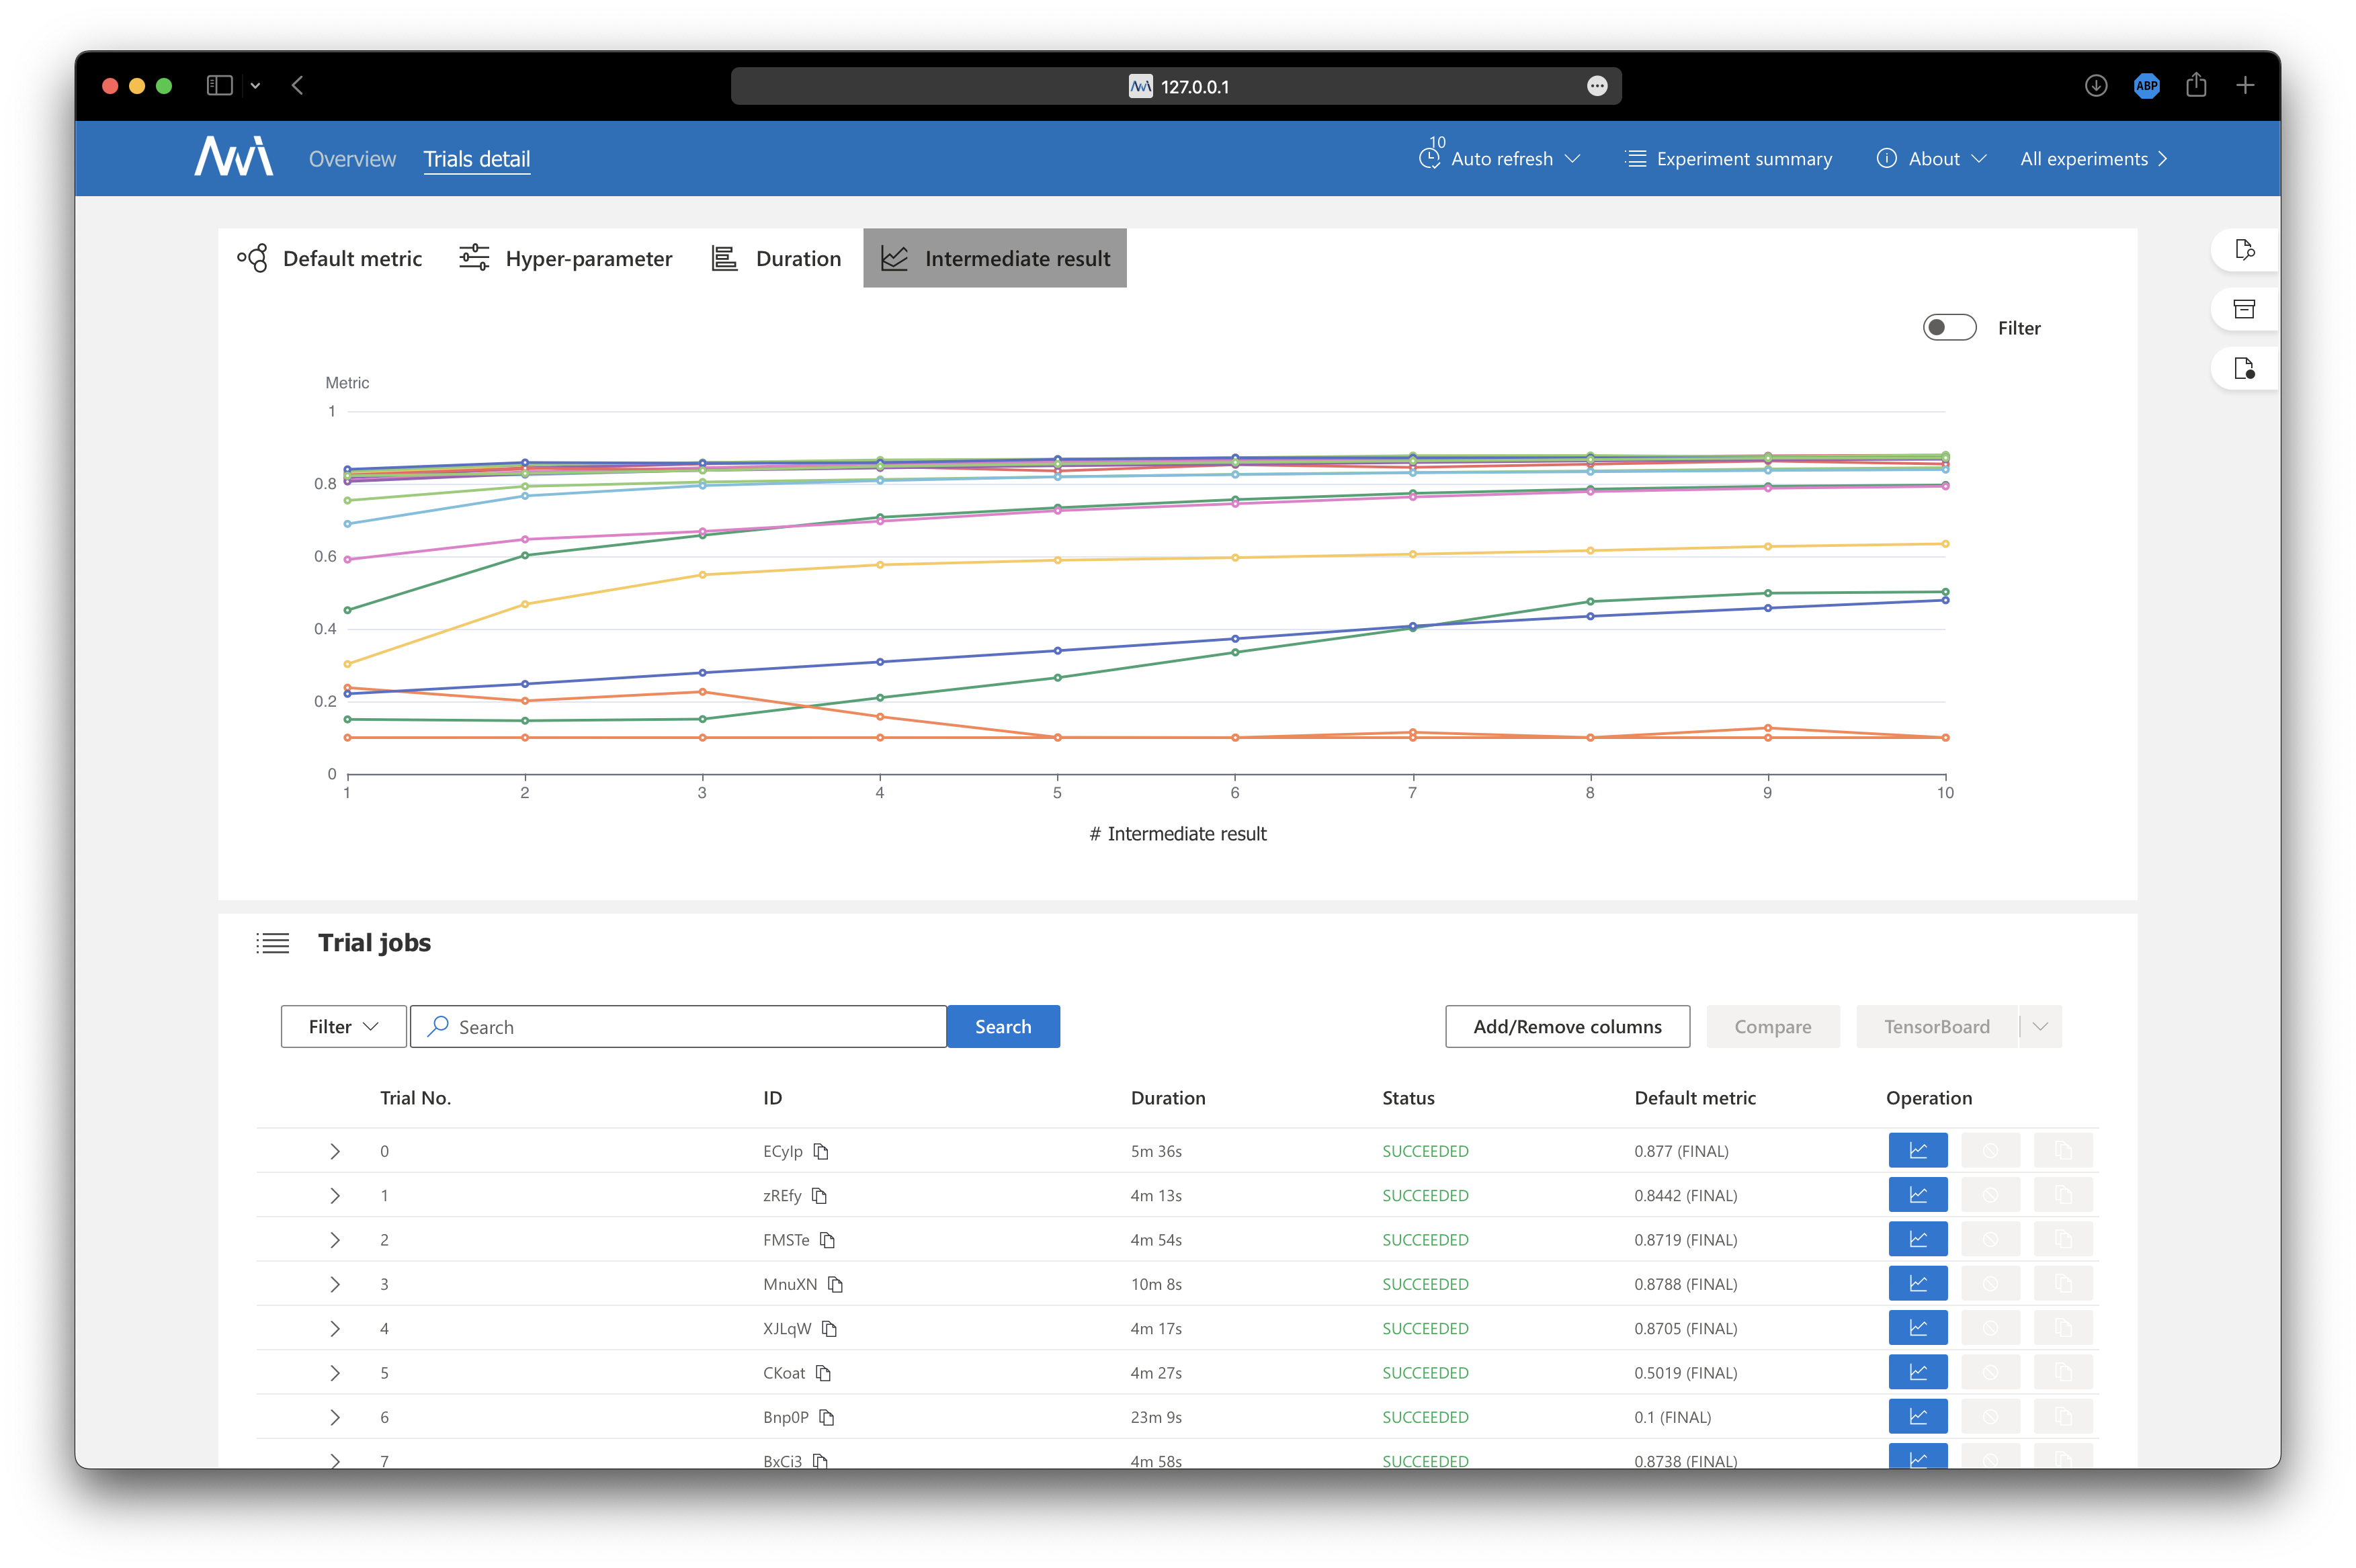
\includegraphics[width=3.5in]{../proj3/figures/mlp_tpe_batch_advanced_intermediate.png}}
    \caption{MLP with TPE Tuner on Learning Rate, Momentum, Feature Size, and Batch Size and Advanced HPO Configurations}
    \label{fig:mlp-tpe-batch-advanced}
\end{figure}
\begin{figure}
    \centerline{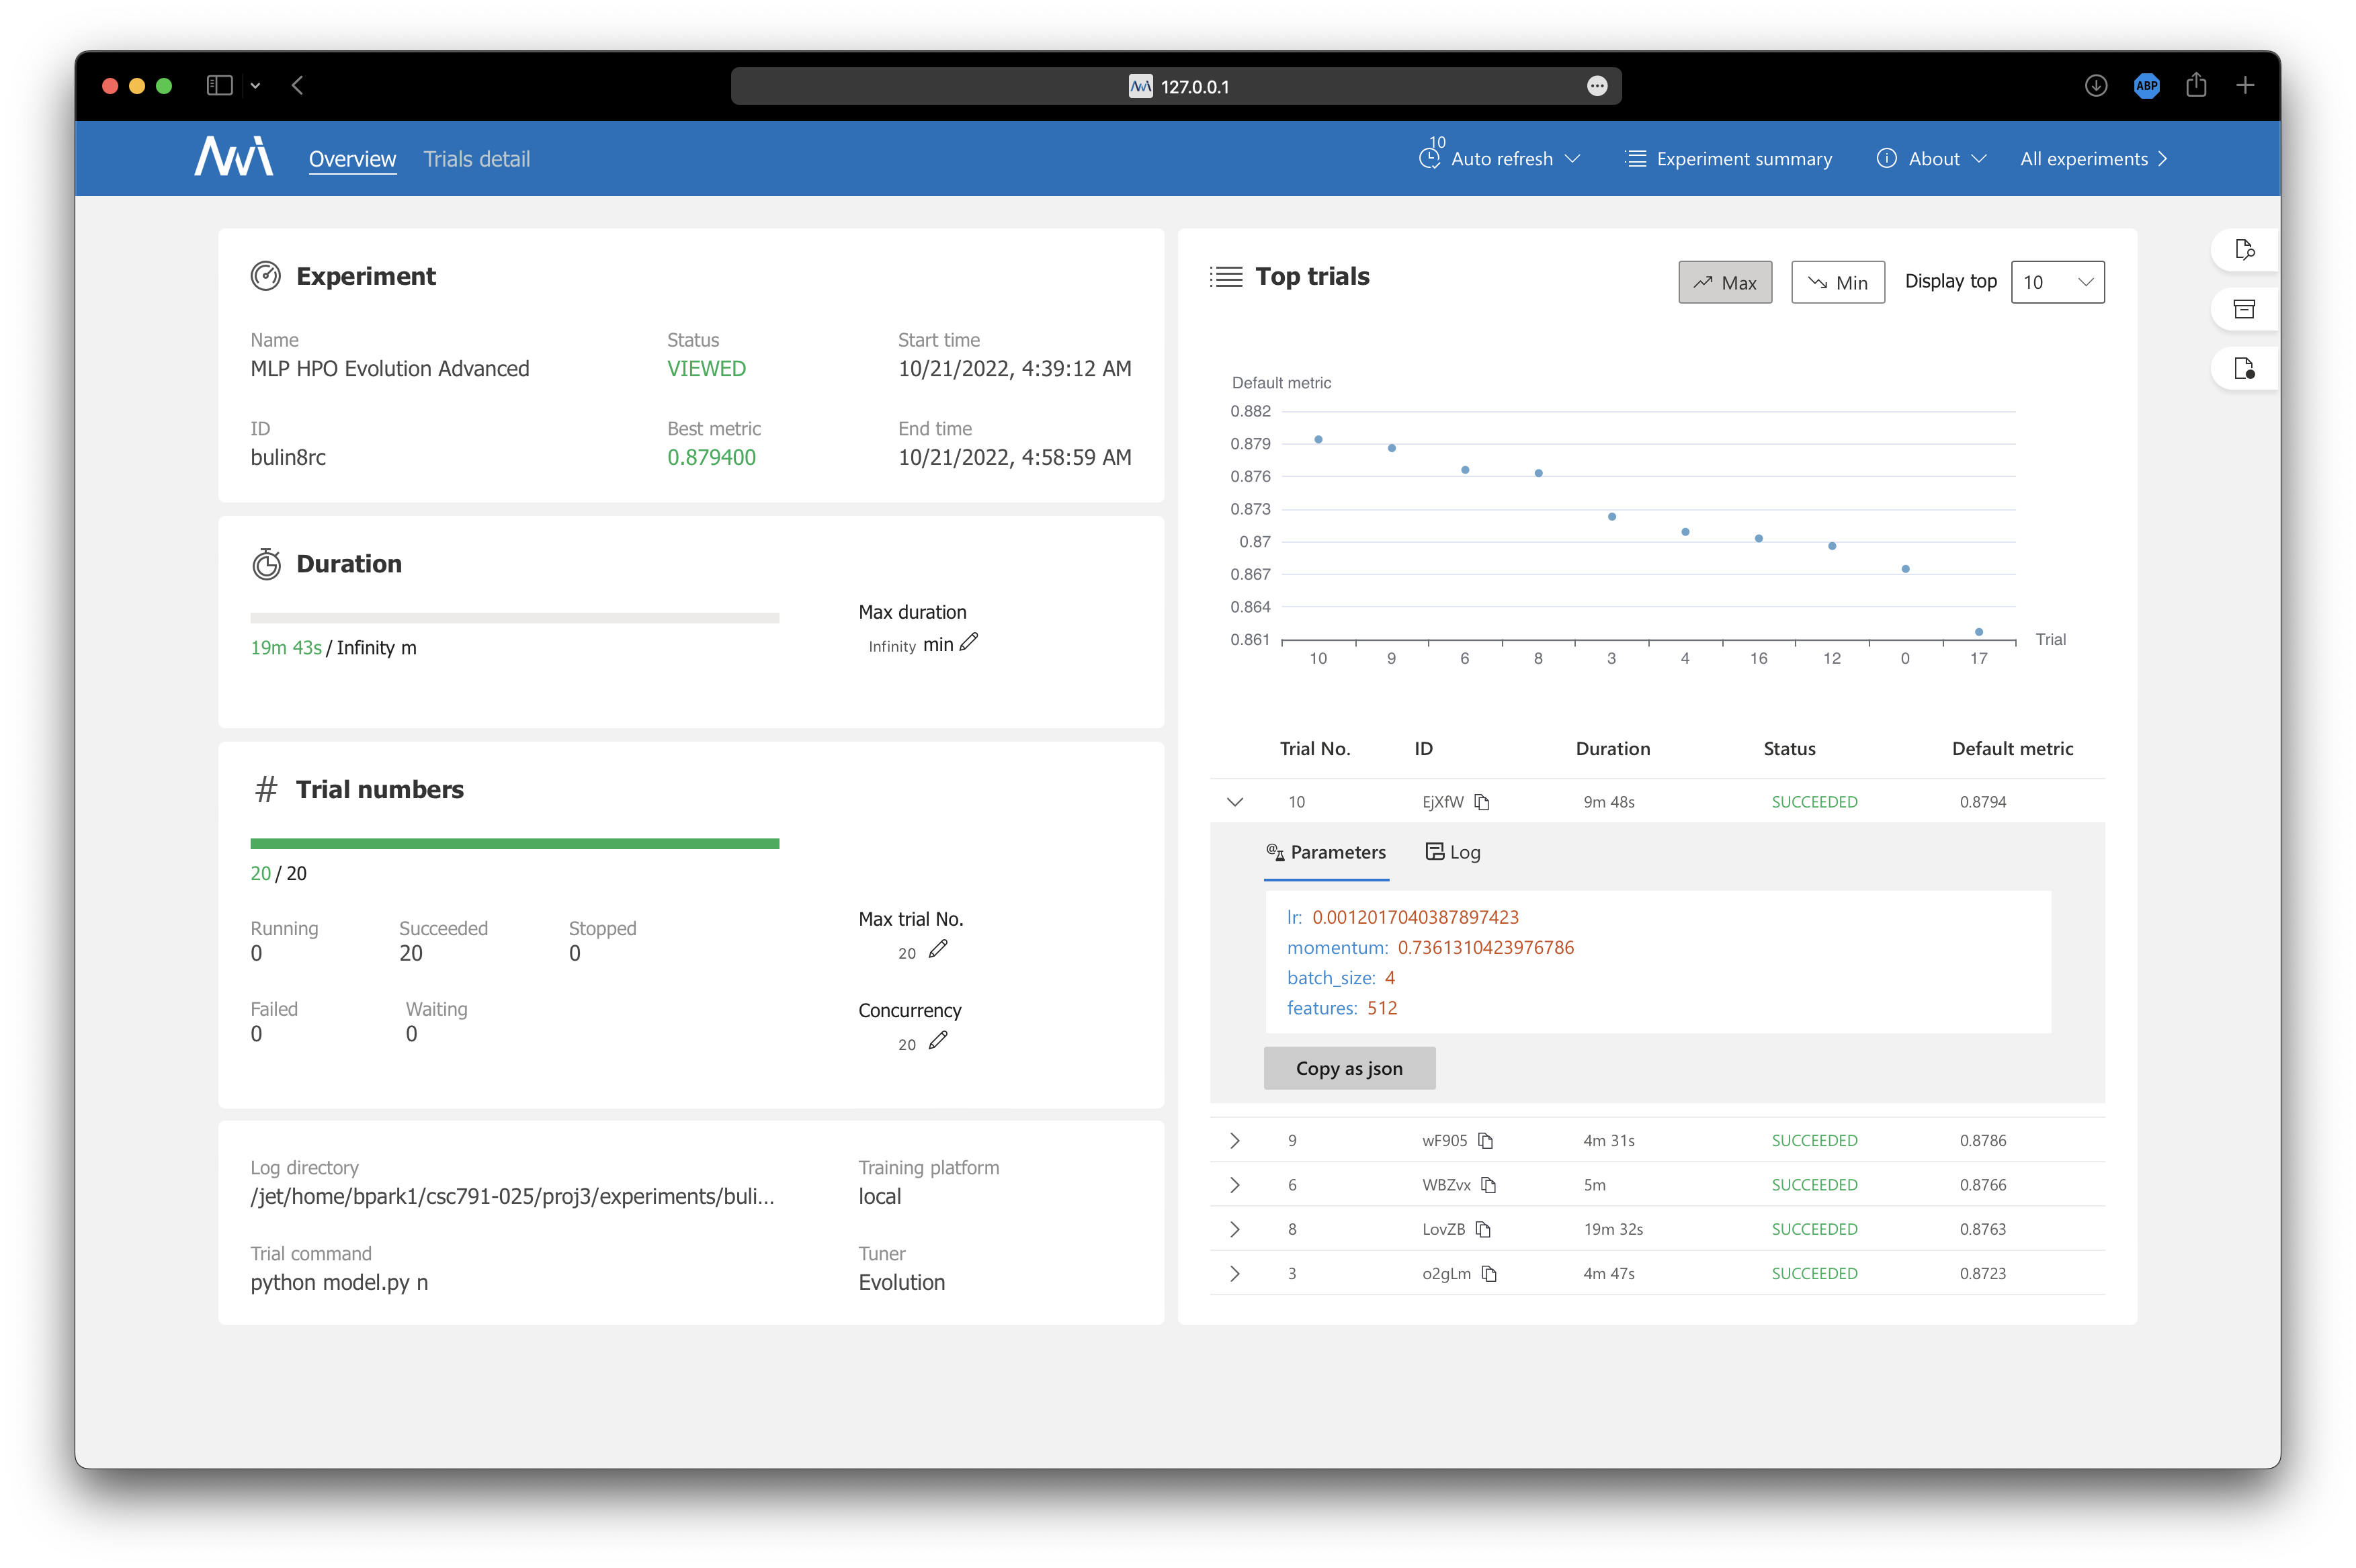
\includegraphics[width=3.5in]{../proj3/figures/mlp_evolution_batch_advanced_overview.png}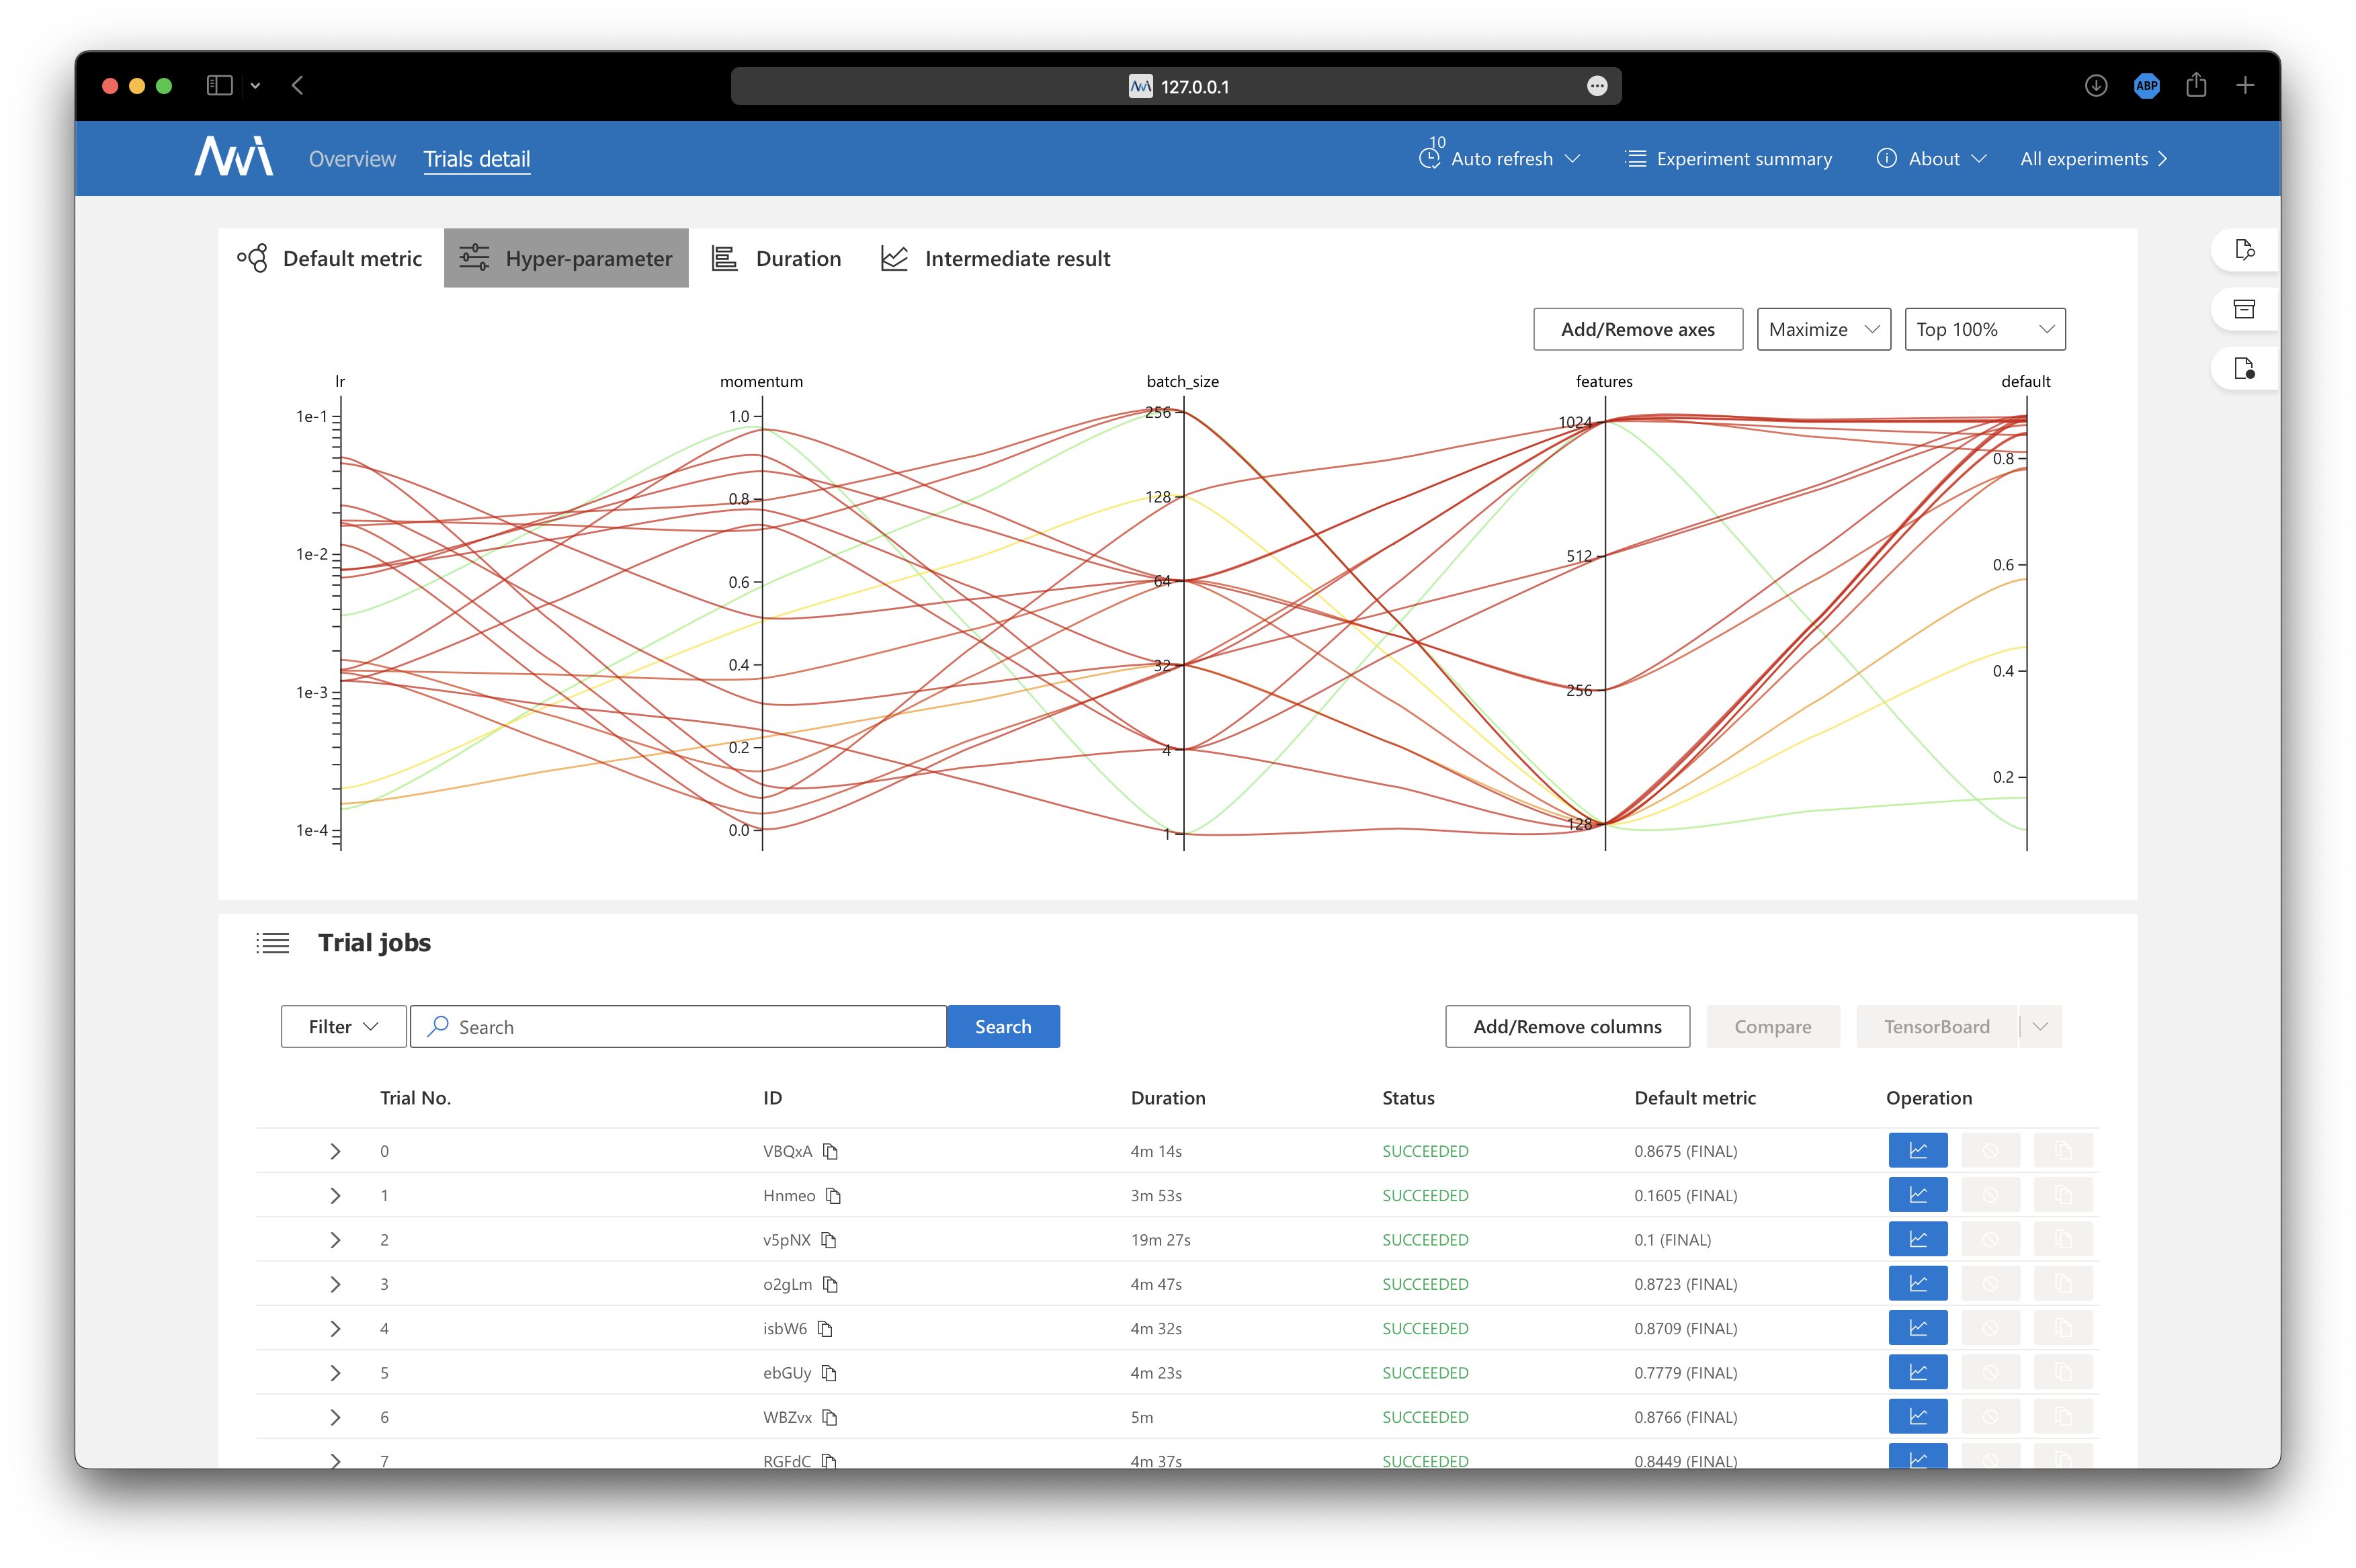
\includegraphics[width=3.5in]{../proj3/figures/mlp_evolution_batch_advanced_hyperparameter.png}}
    \centerline{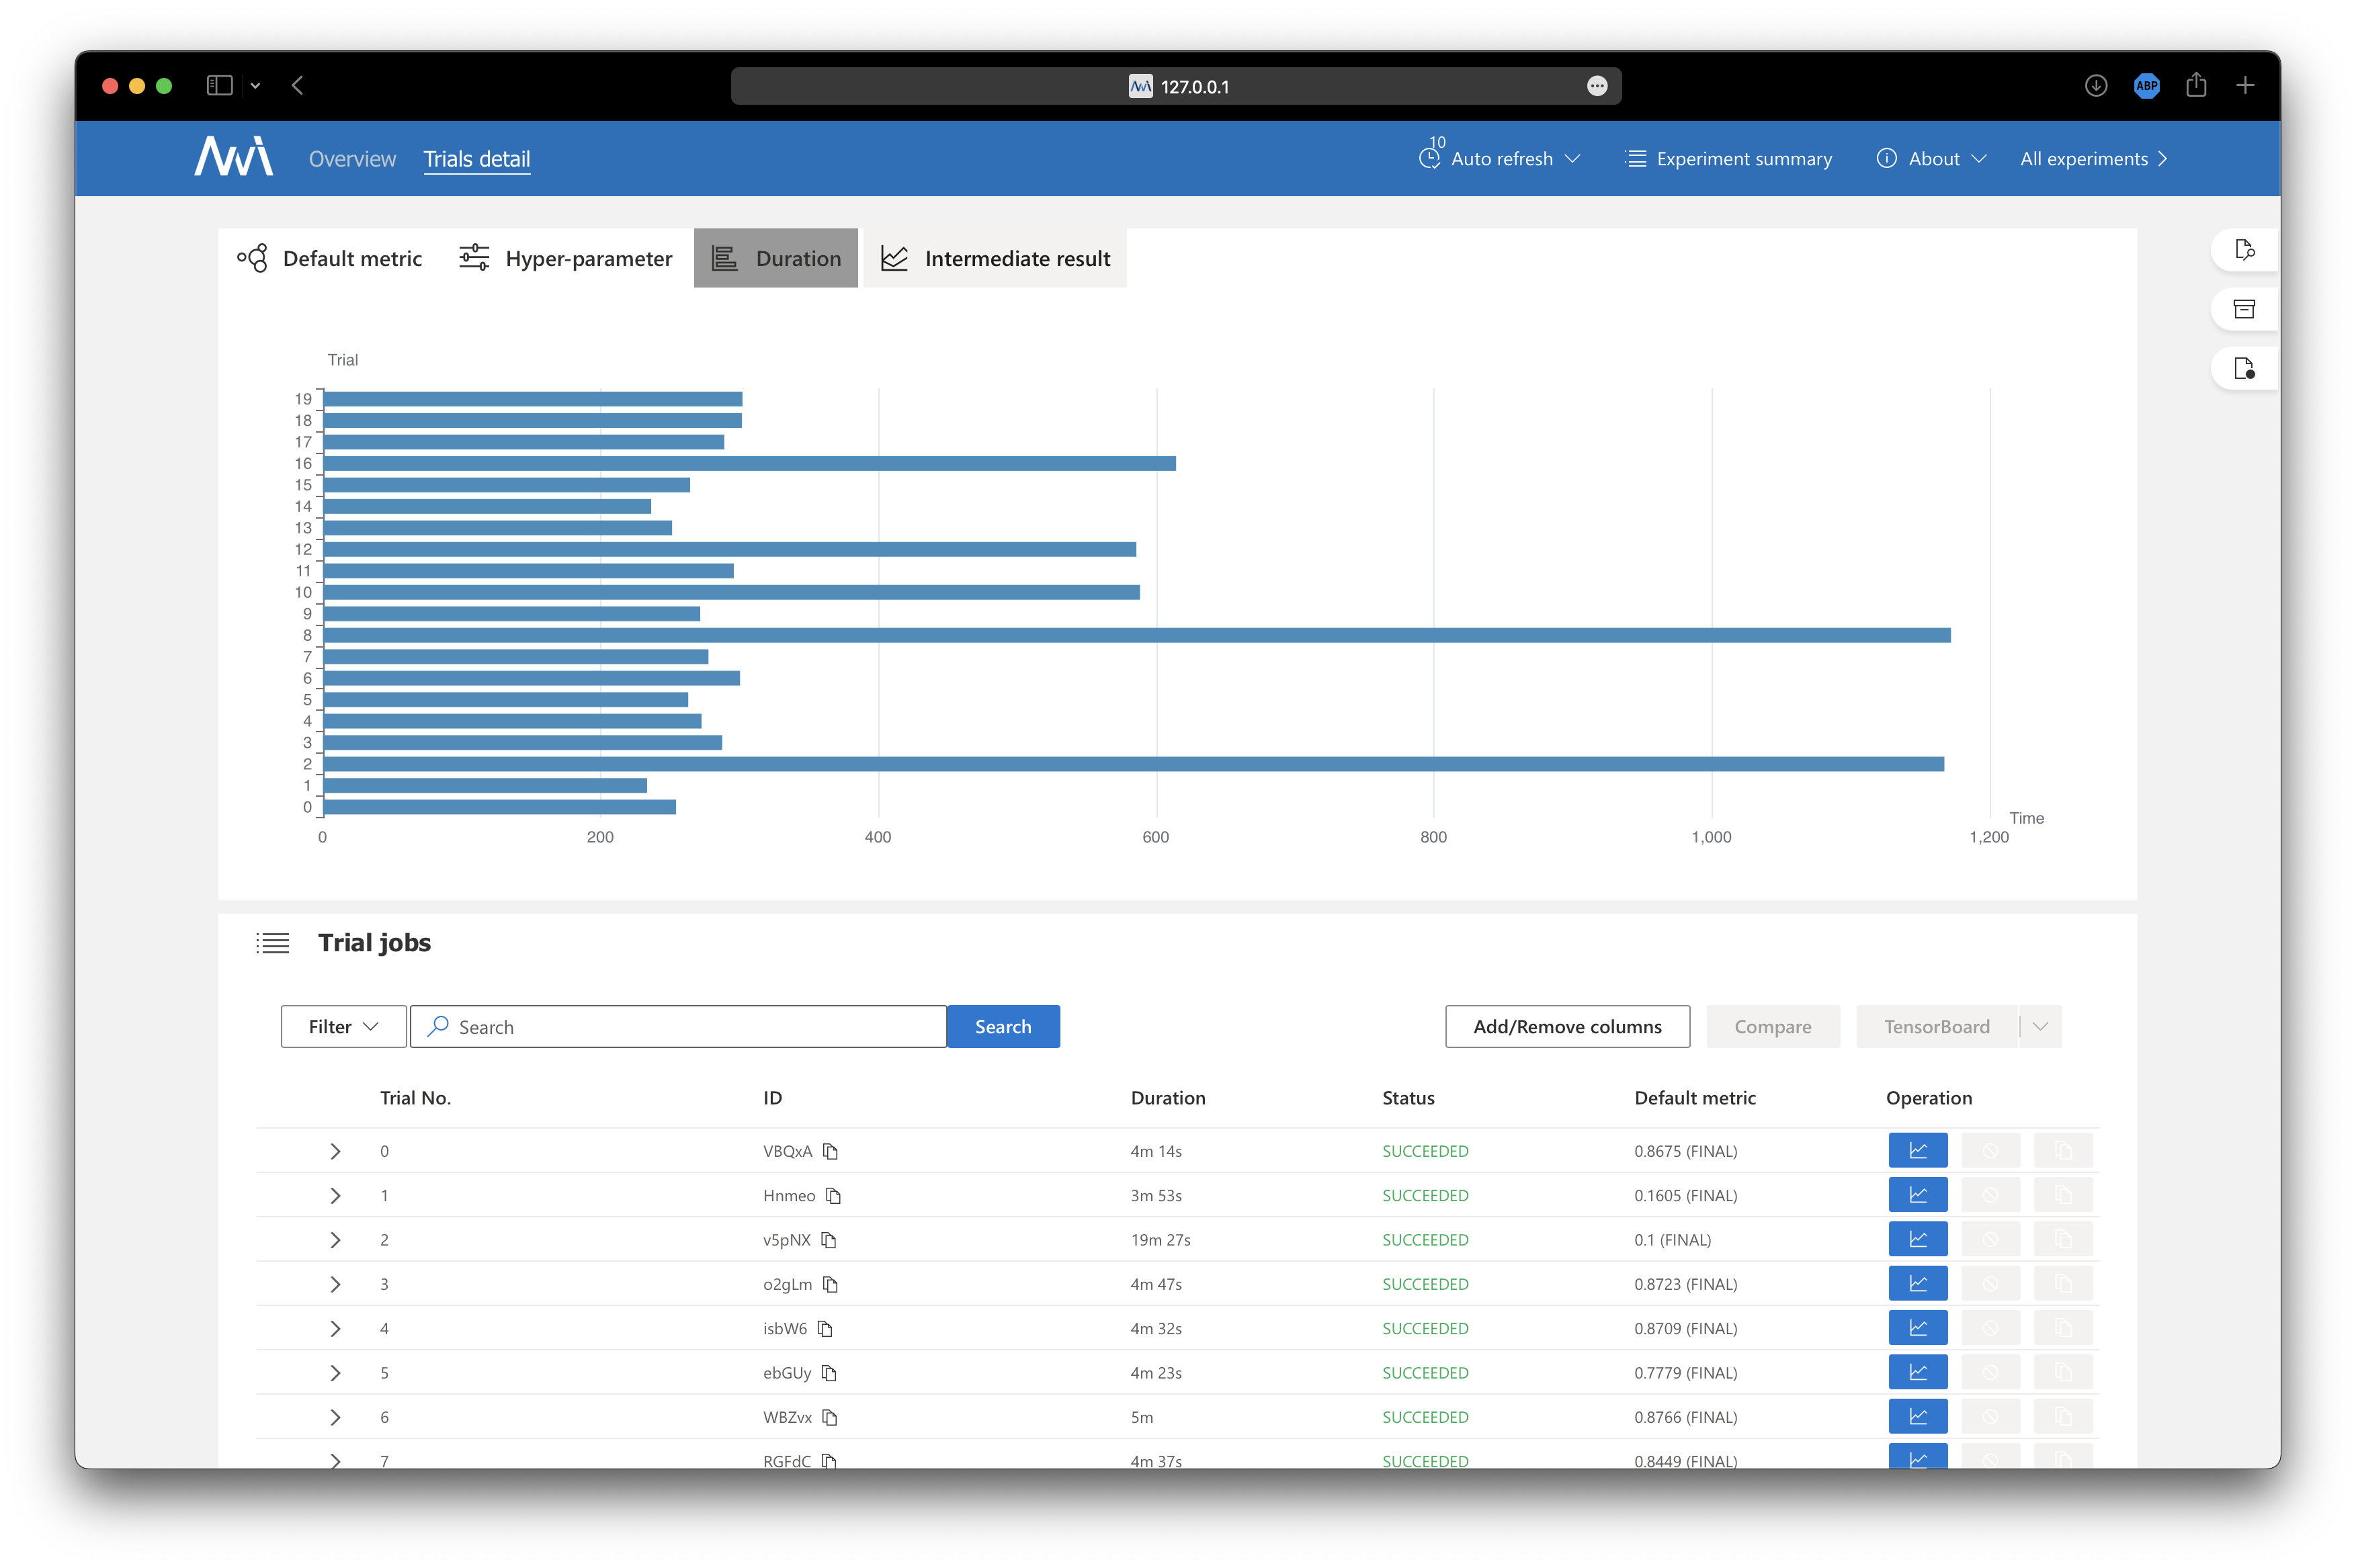
\includegraphics[width=3.5in]{../proj3/figures/mlp_evolution_batch_advanced_latency.png}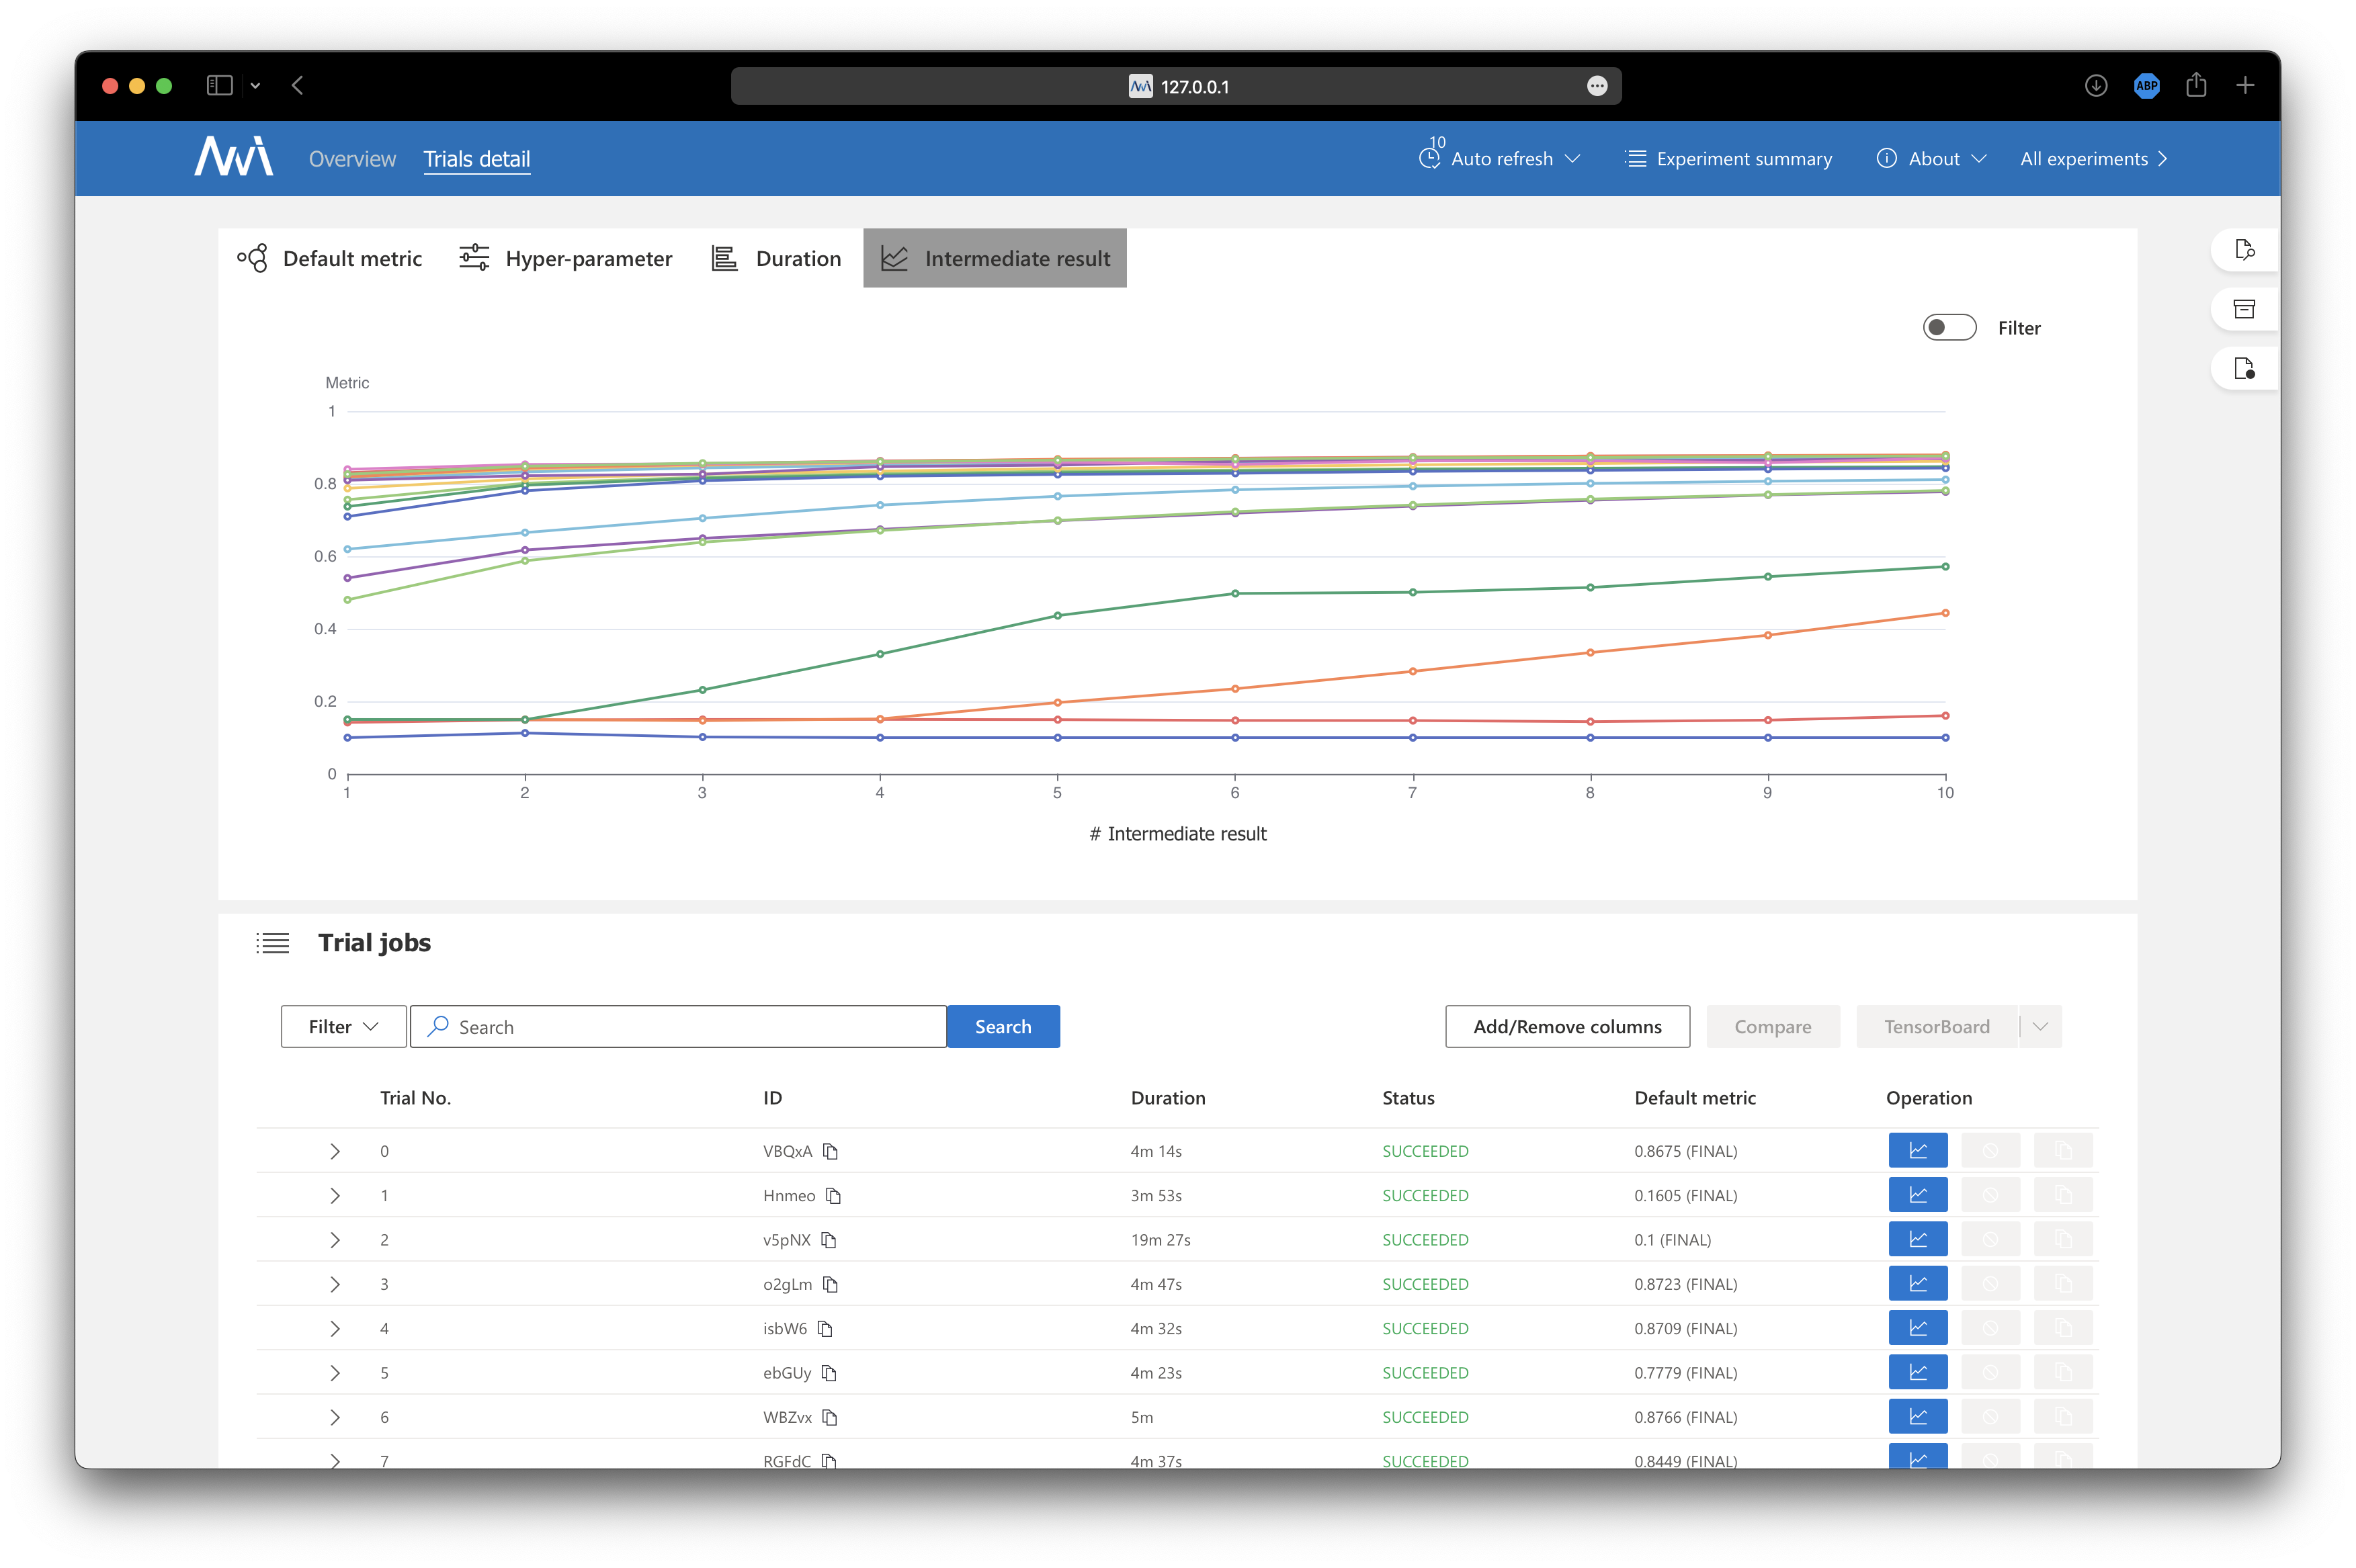
\includegraphics[width=3.5in]{../proj3/figures/mlp_evolution_batch_advanced_intermediate.png}}
    \caption{MLP with Evolution Tuner on Learning Rate, Momentum, Feature Size, and Batch Size and Advanced HPO Configurations}
    \label{fig:mlp-evolution-batch-advanced}
\end{figure}
\begin{figure}
    \centerline{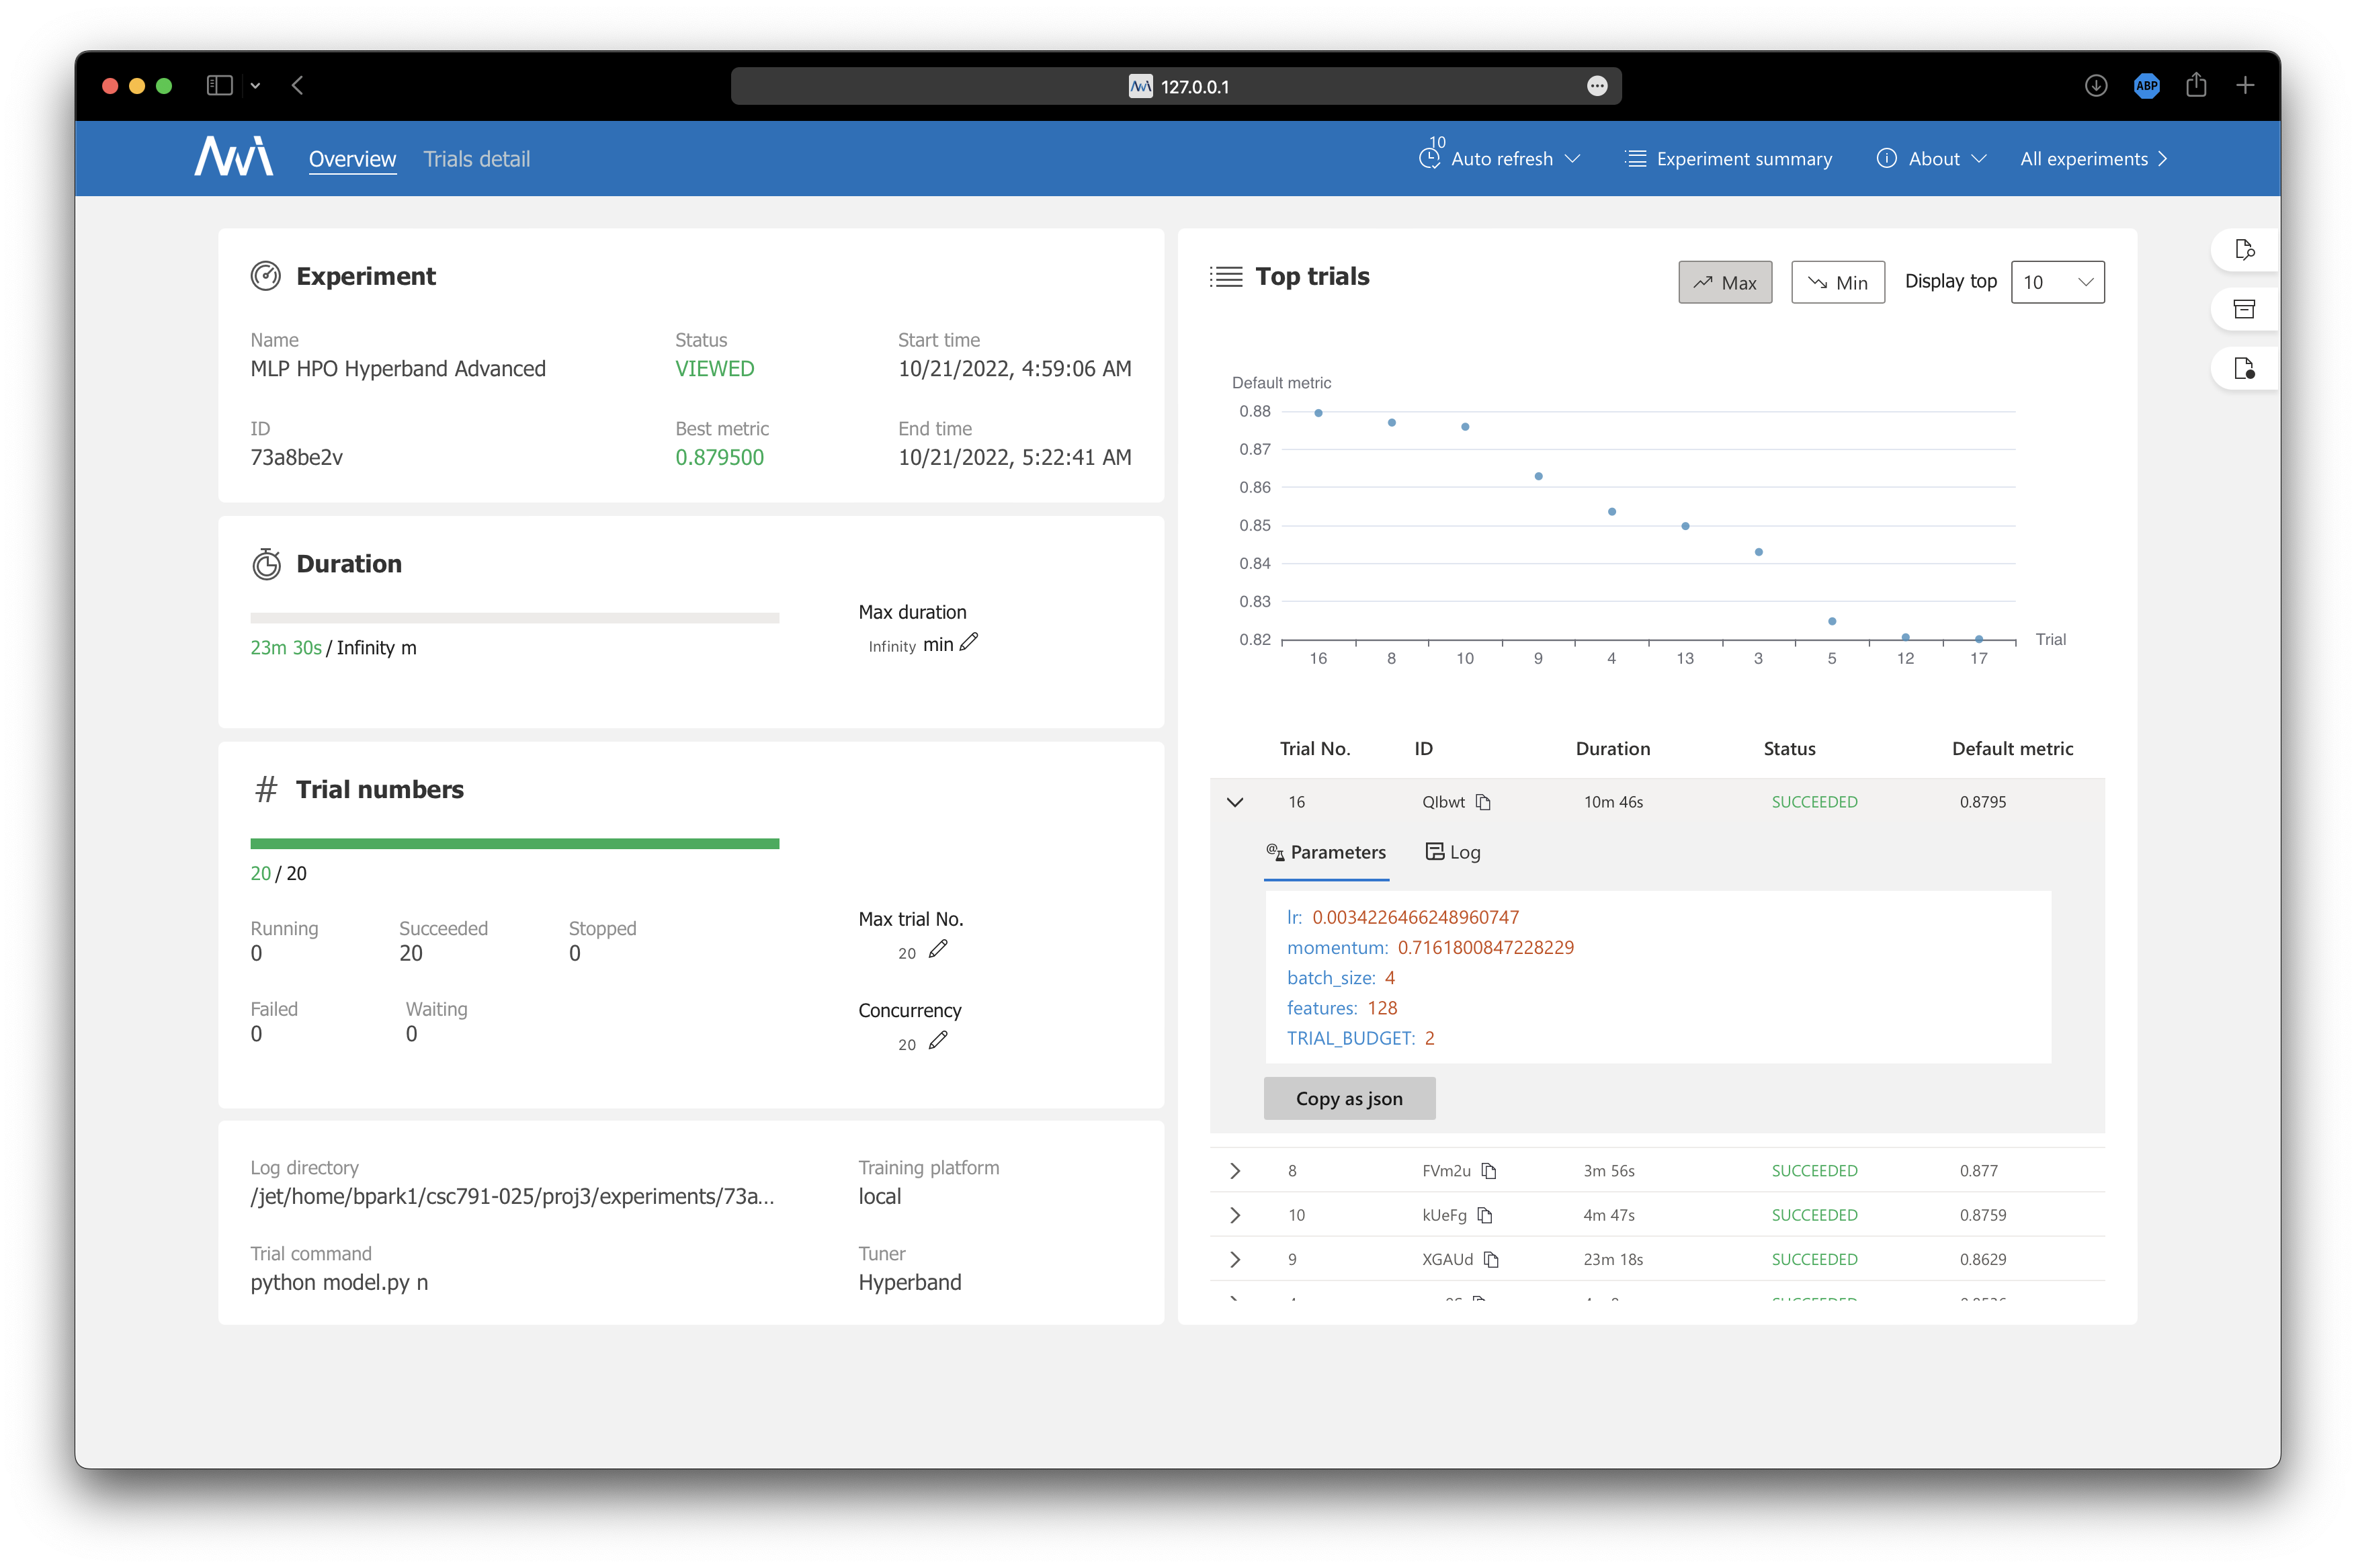
\includegraphics[width=3.5in]{../proj3/figures/mlp_hyperband_batch_advanced_overview.png}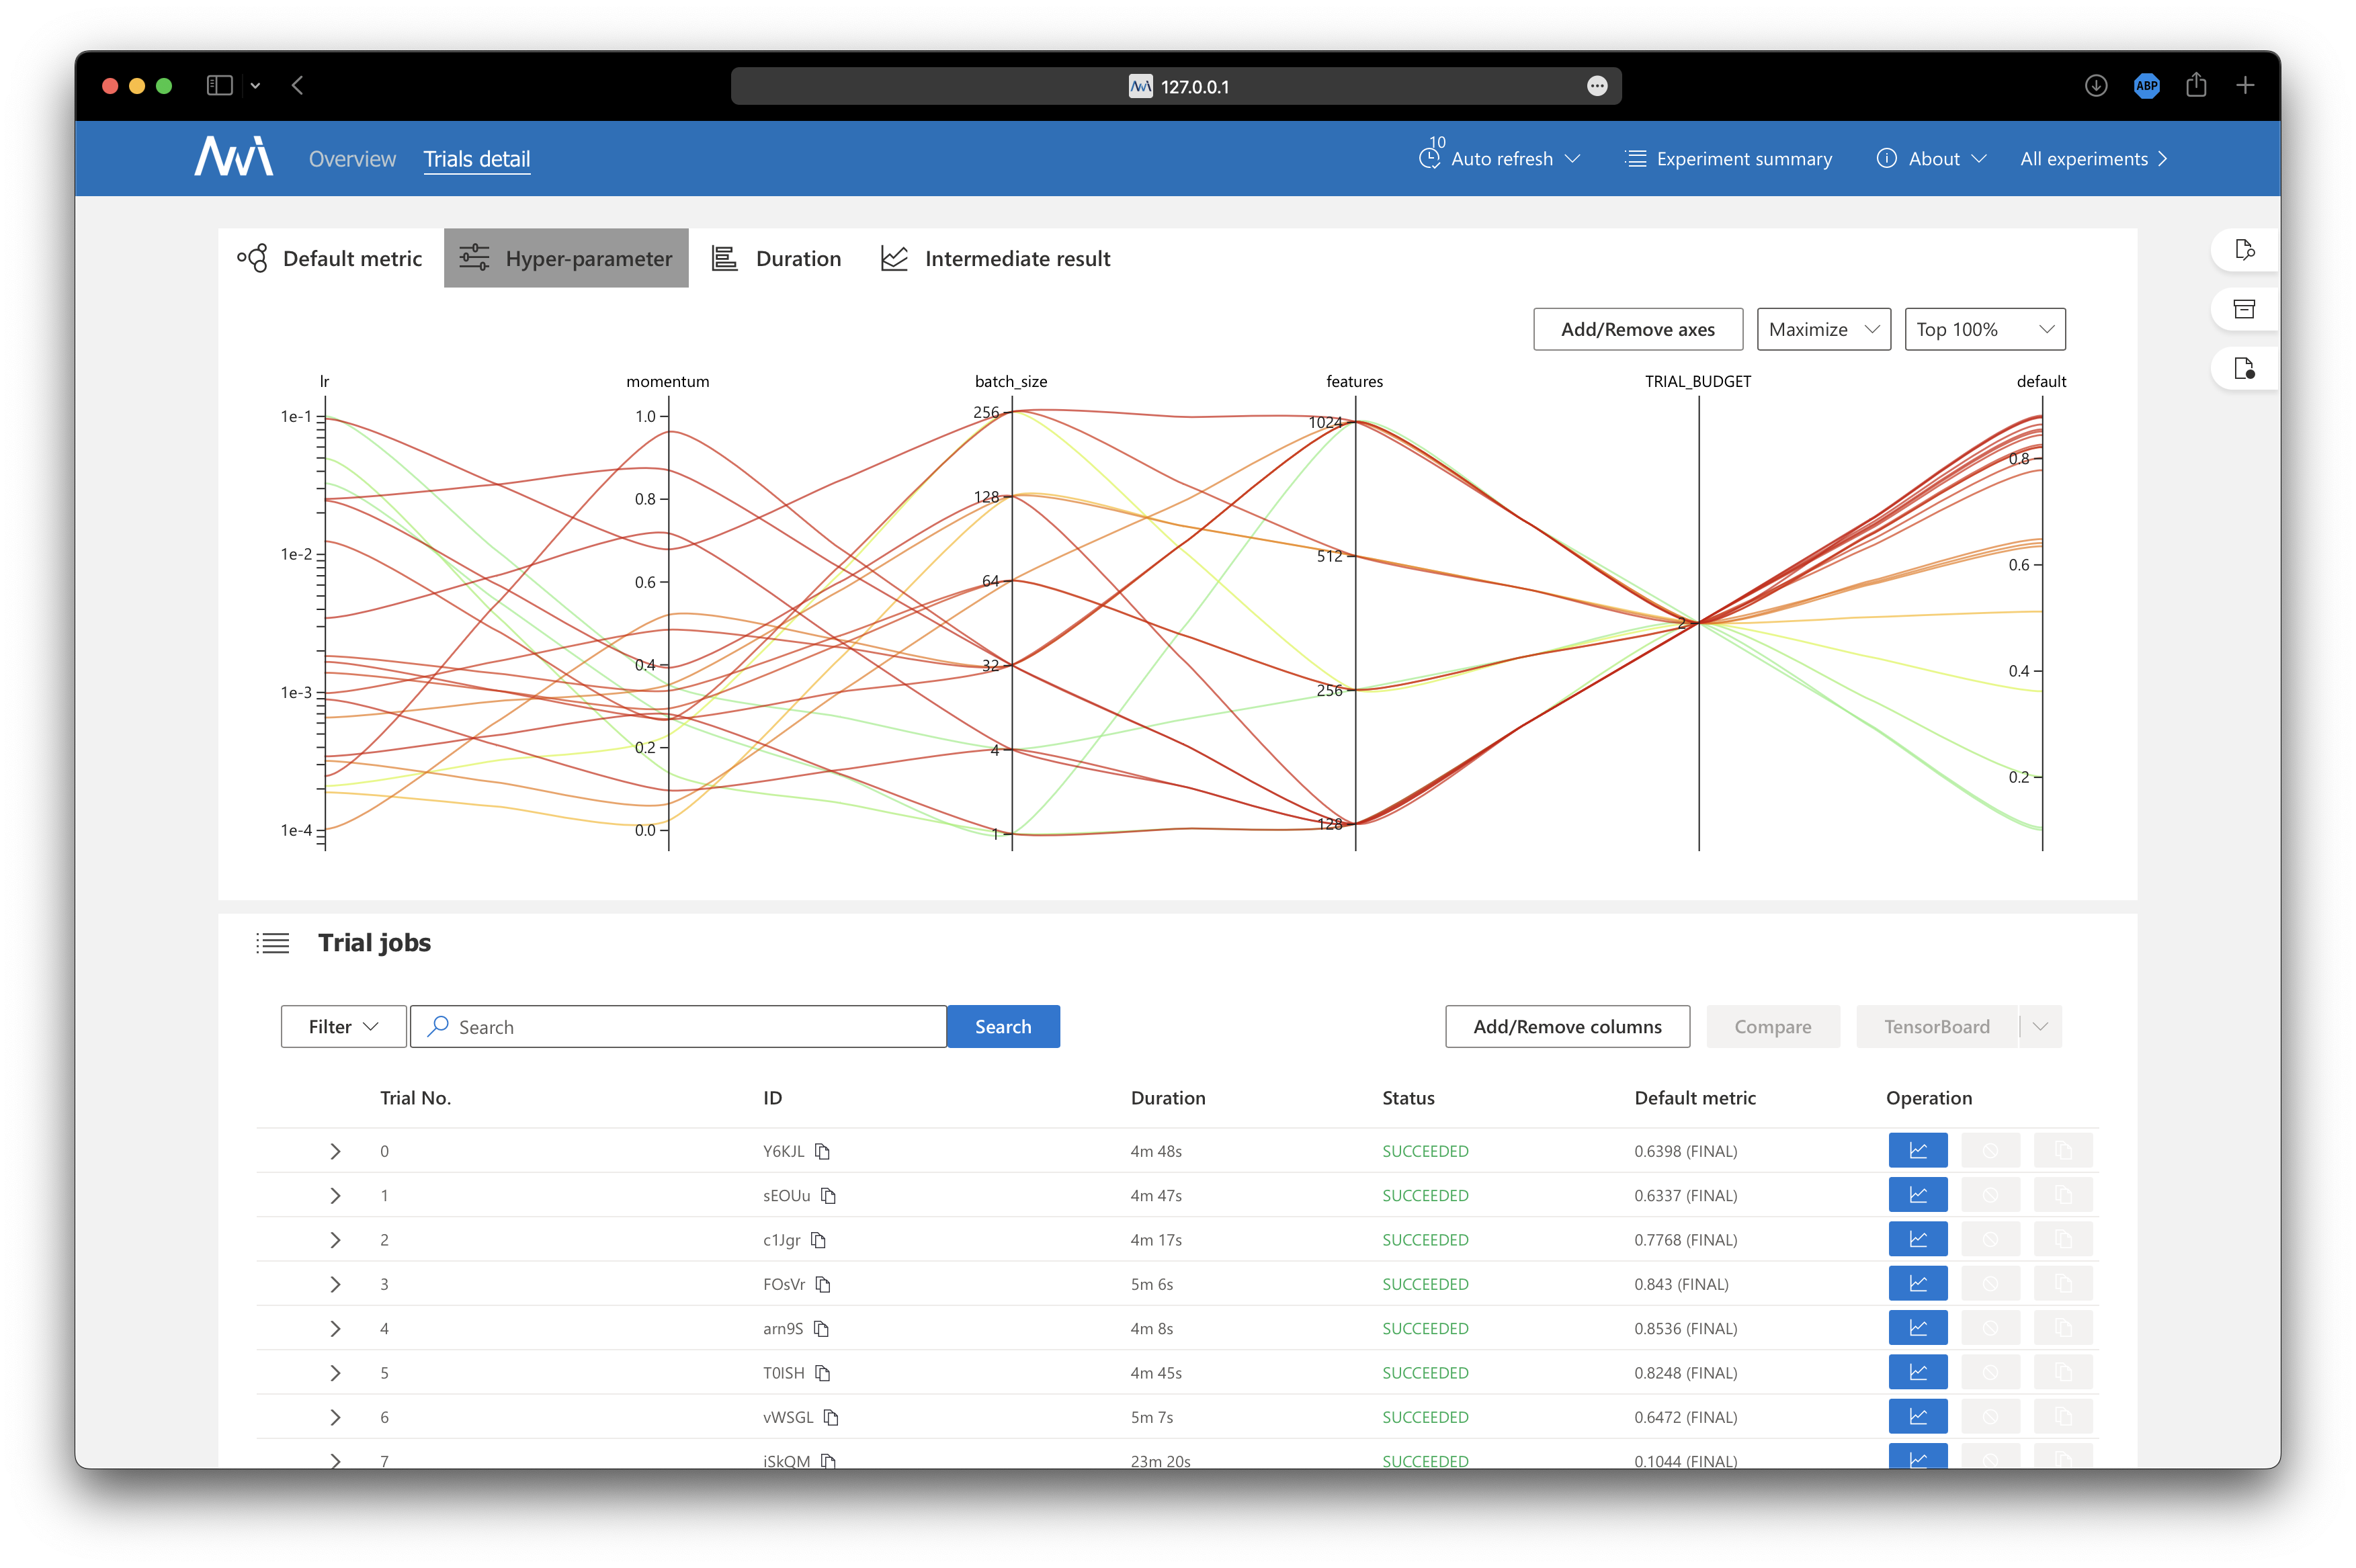
\includegraphics[width=3.5in]{../proj3/figures/mlp_hyperband_batch_advanced_hyperparameter.png}}
    \centerline{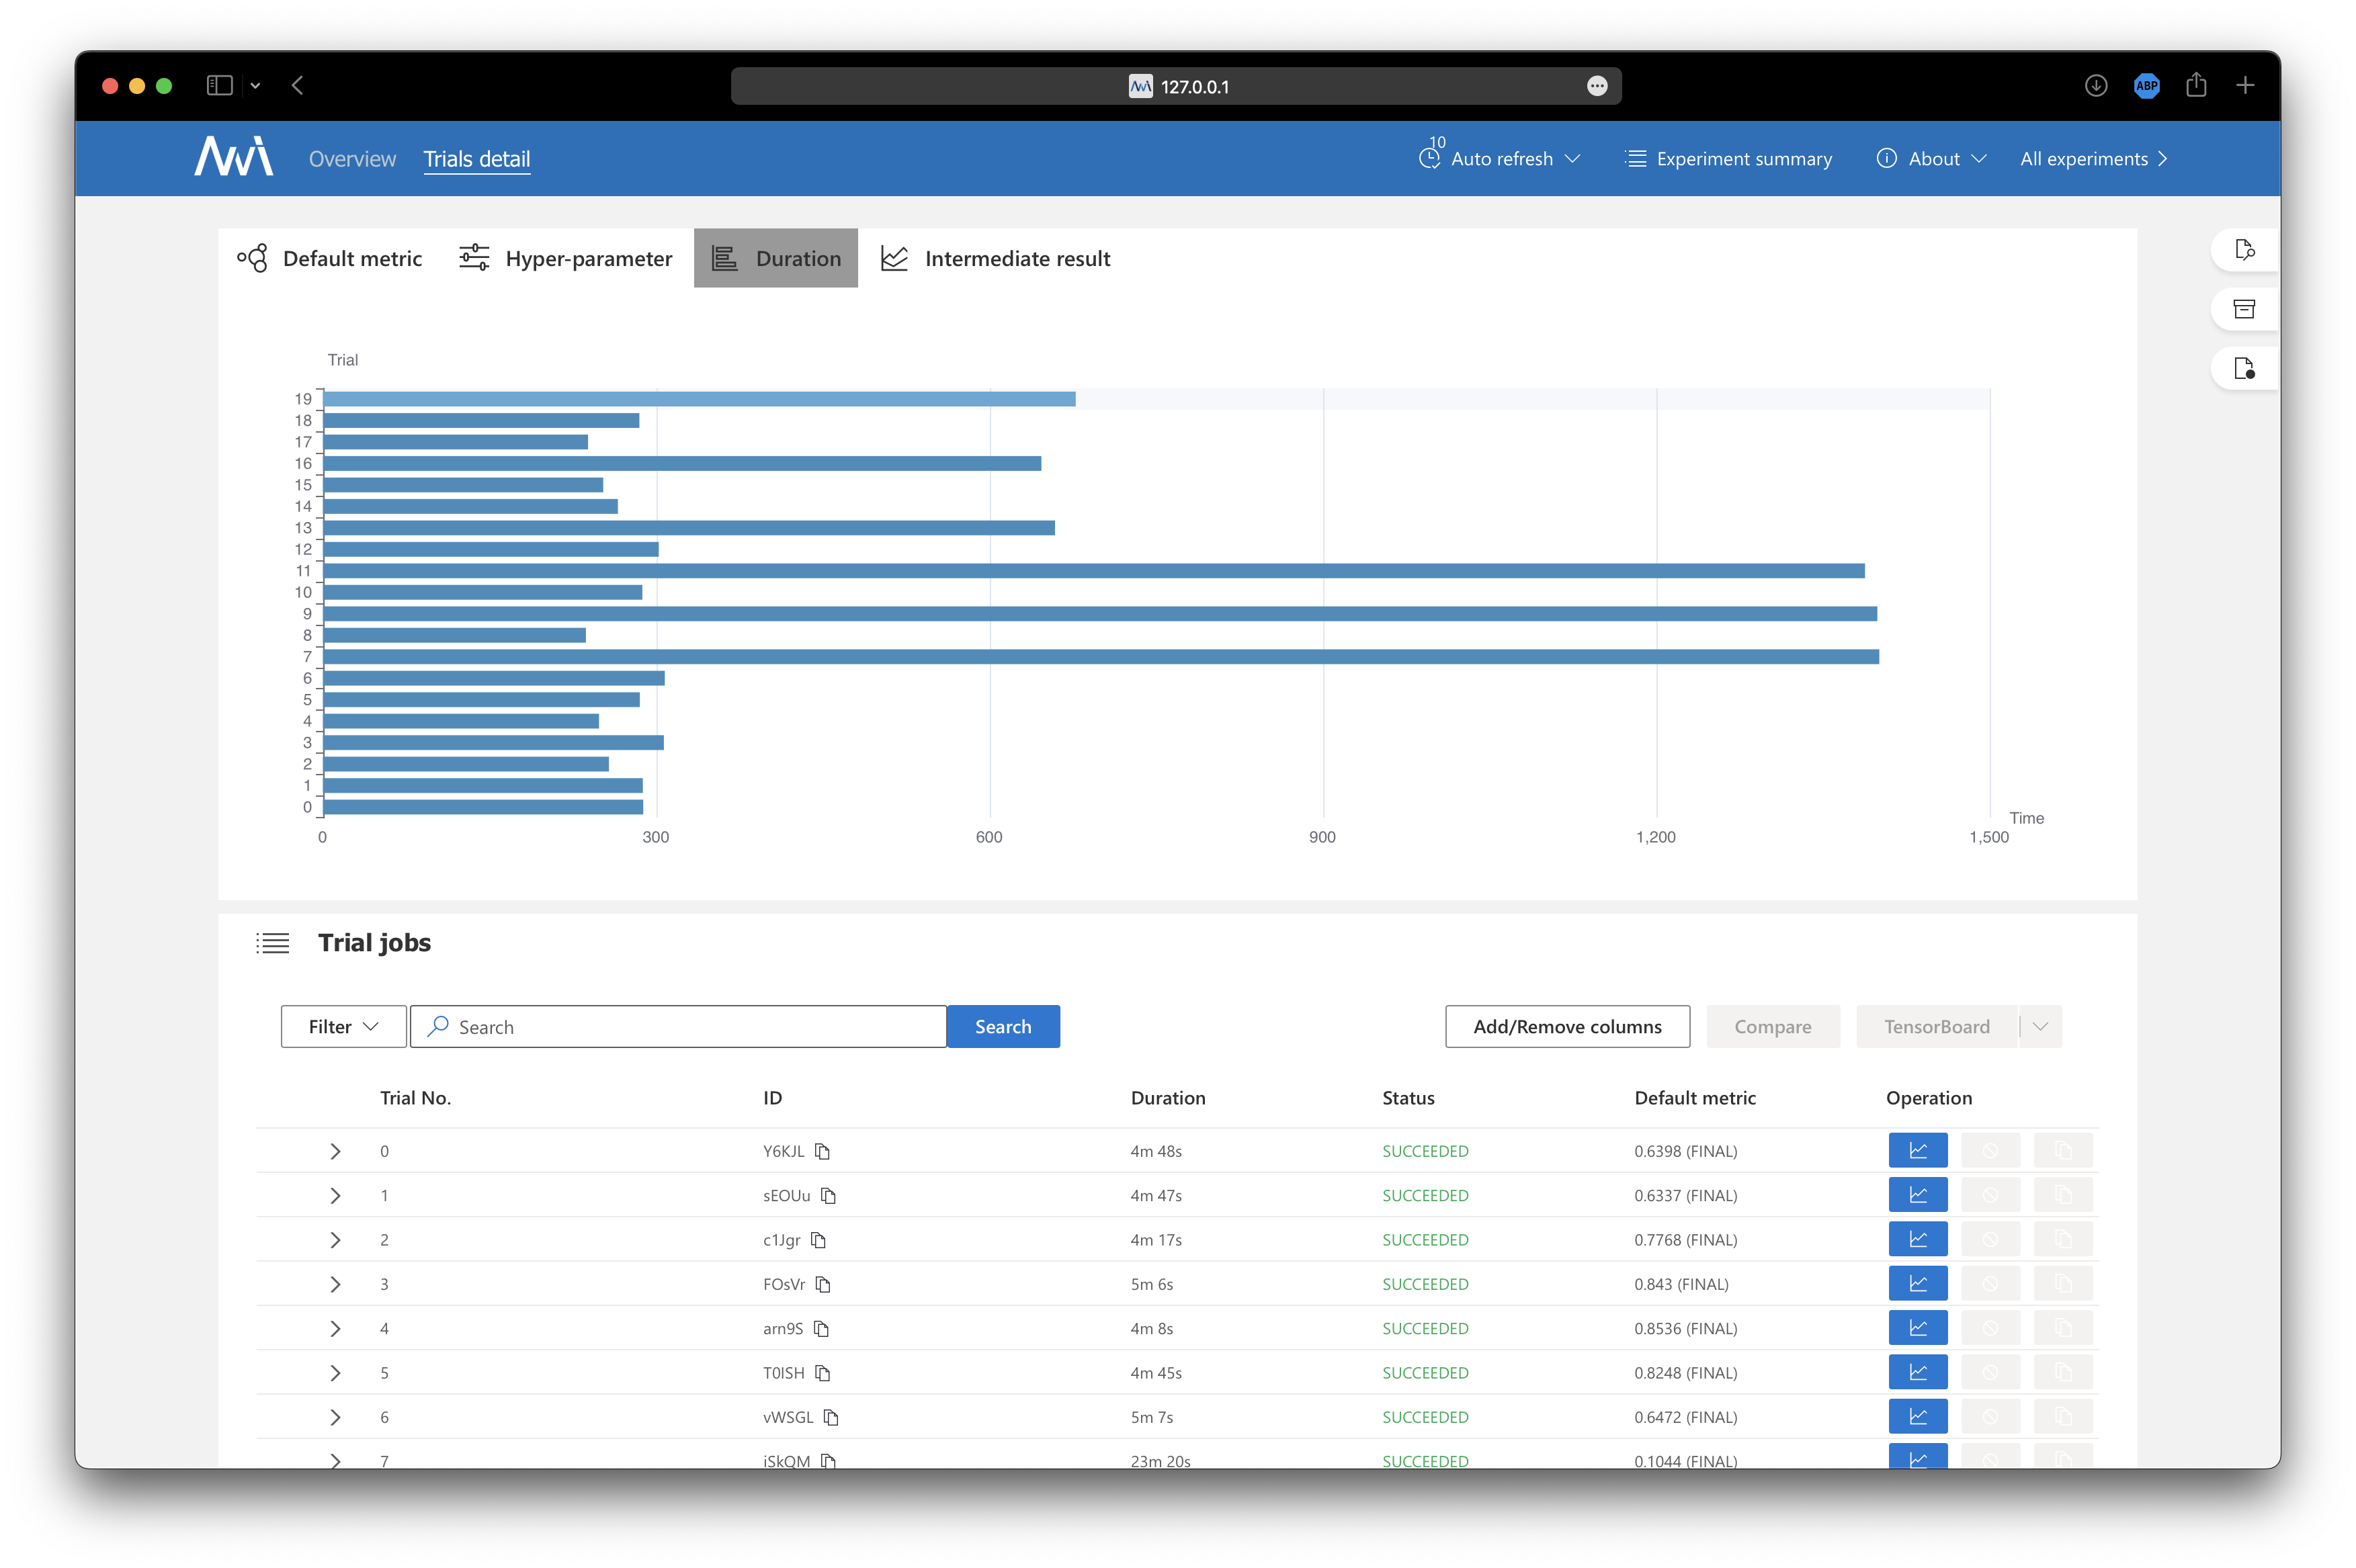
\includegraphics[width=3.5in]{../proj3/figures/mlp_hyperband_batch_advanced_latency.png}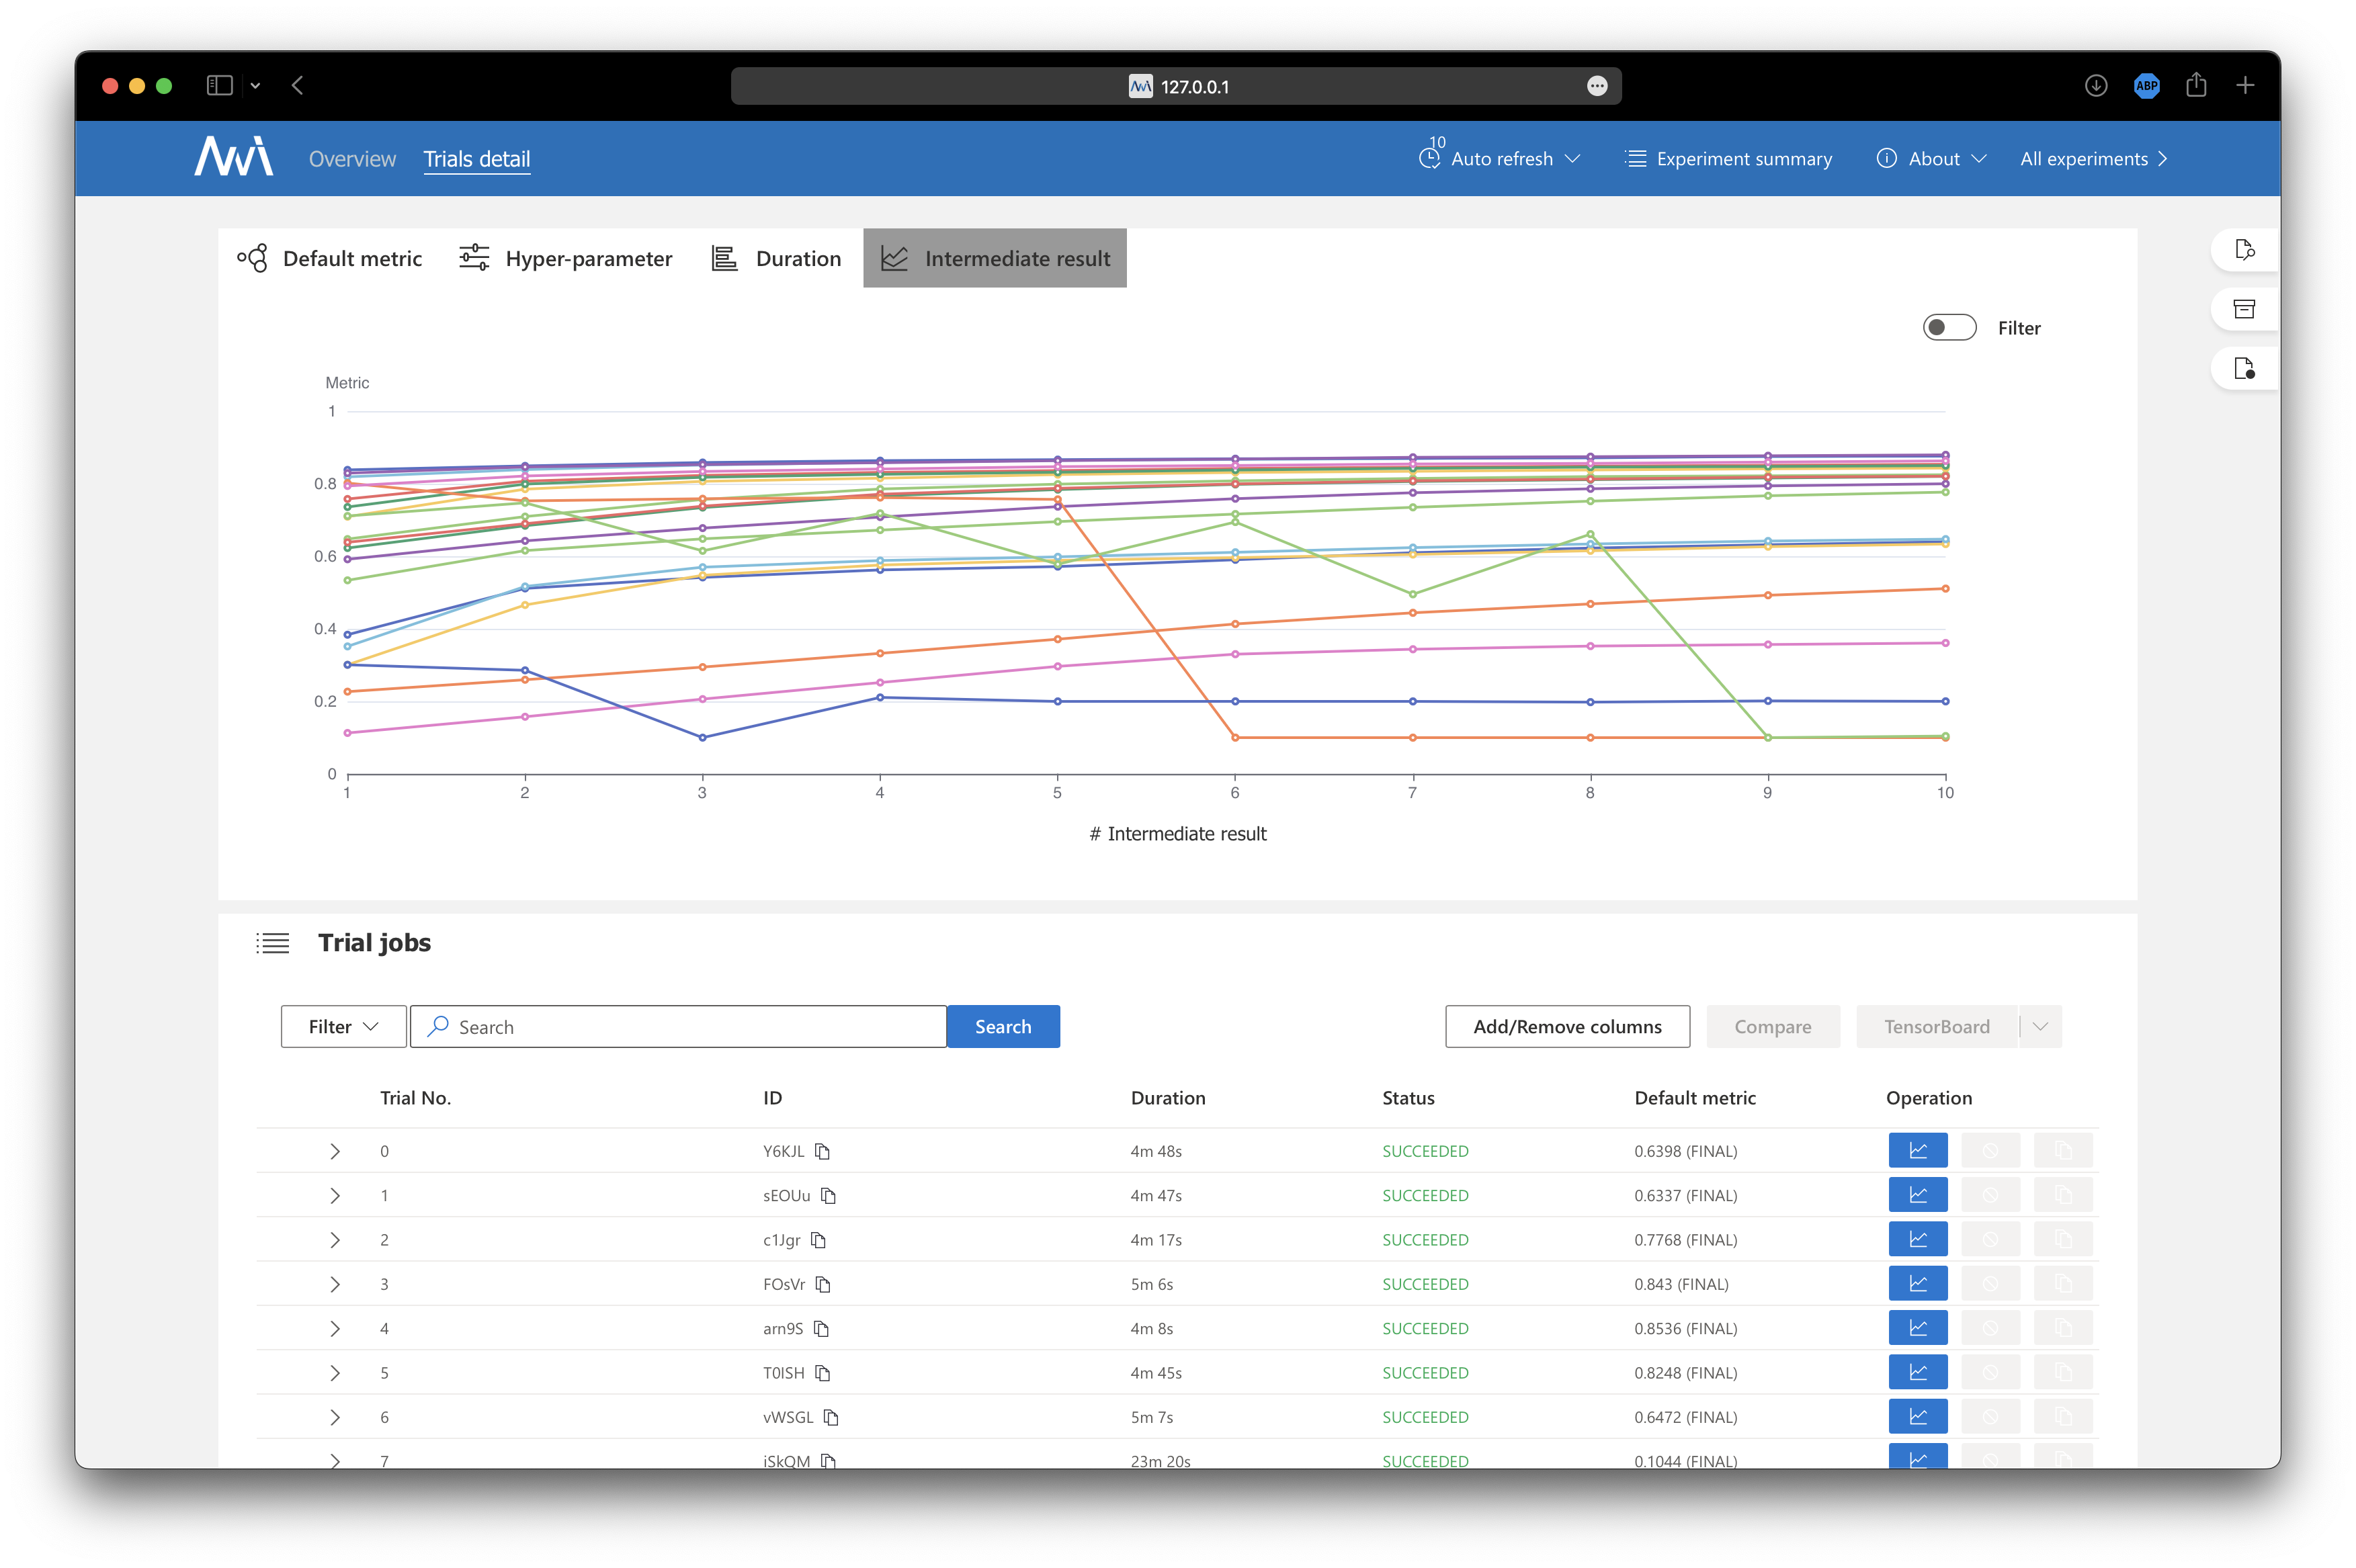
\includegraphics[width=3.5in]{../proj3/figures/mlp_hyperband_batch_advanced_intermediate.png}}
    \caption{MLP with Hyperband Tuner on Learning Rate, Momentum, Feature Size, and Batch Size and Advanced HPO Configurations}
    \label{fig:mlp-hyperband-batch-advanced}
\end{figure}
\begin{figure}
    \centerline{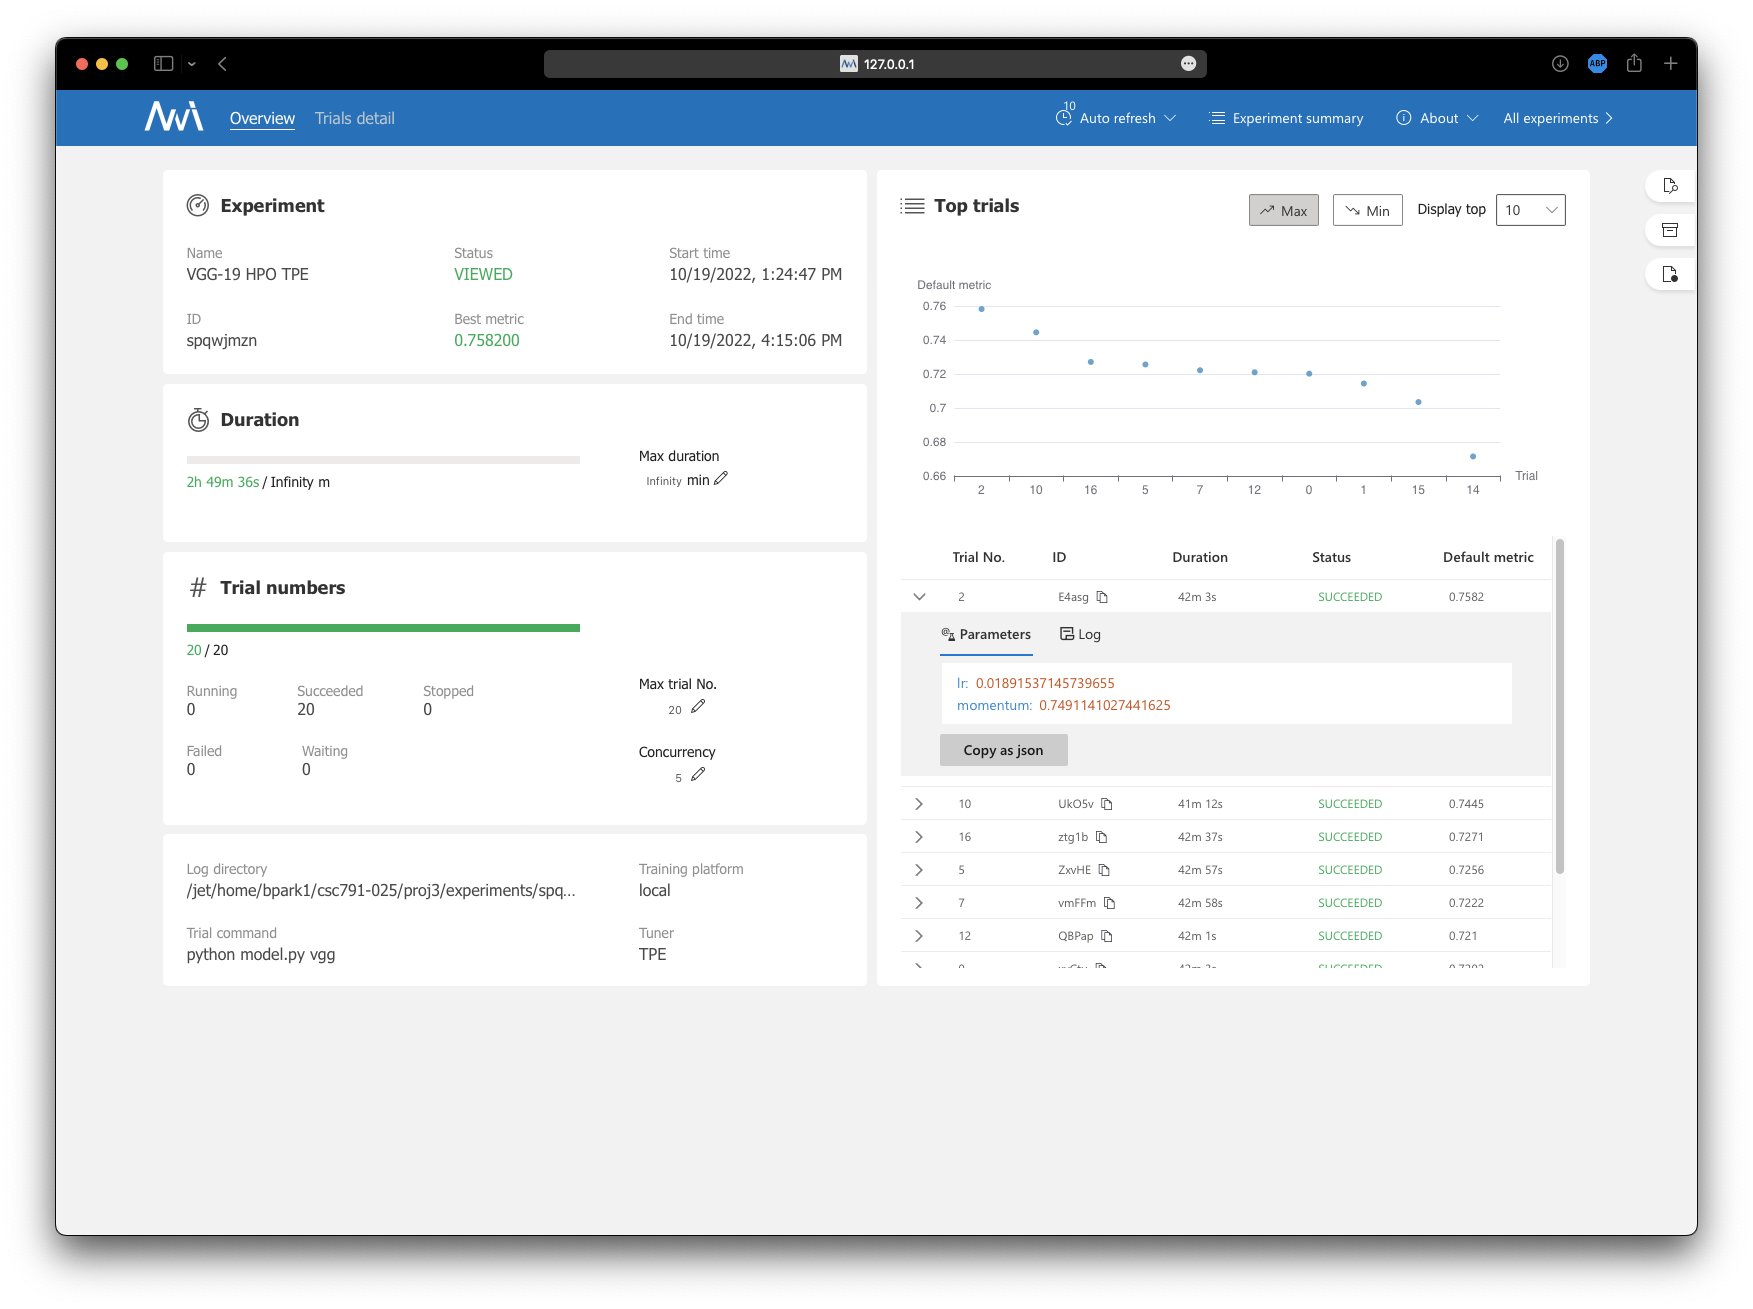
\includegraphics[width=3.5in]{../proj3/figures/vgg_tpe_overview.png}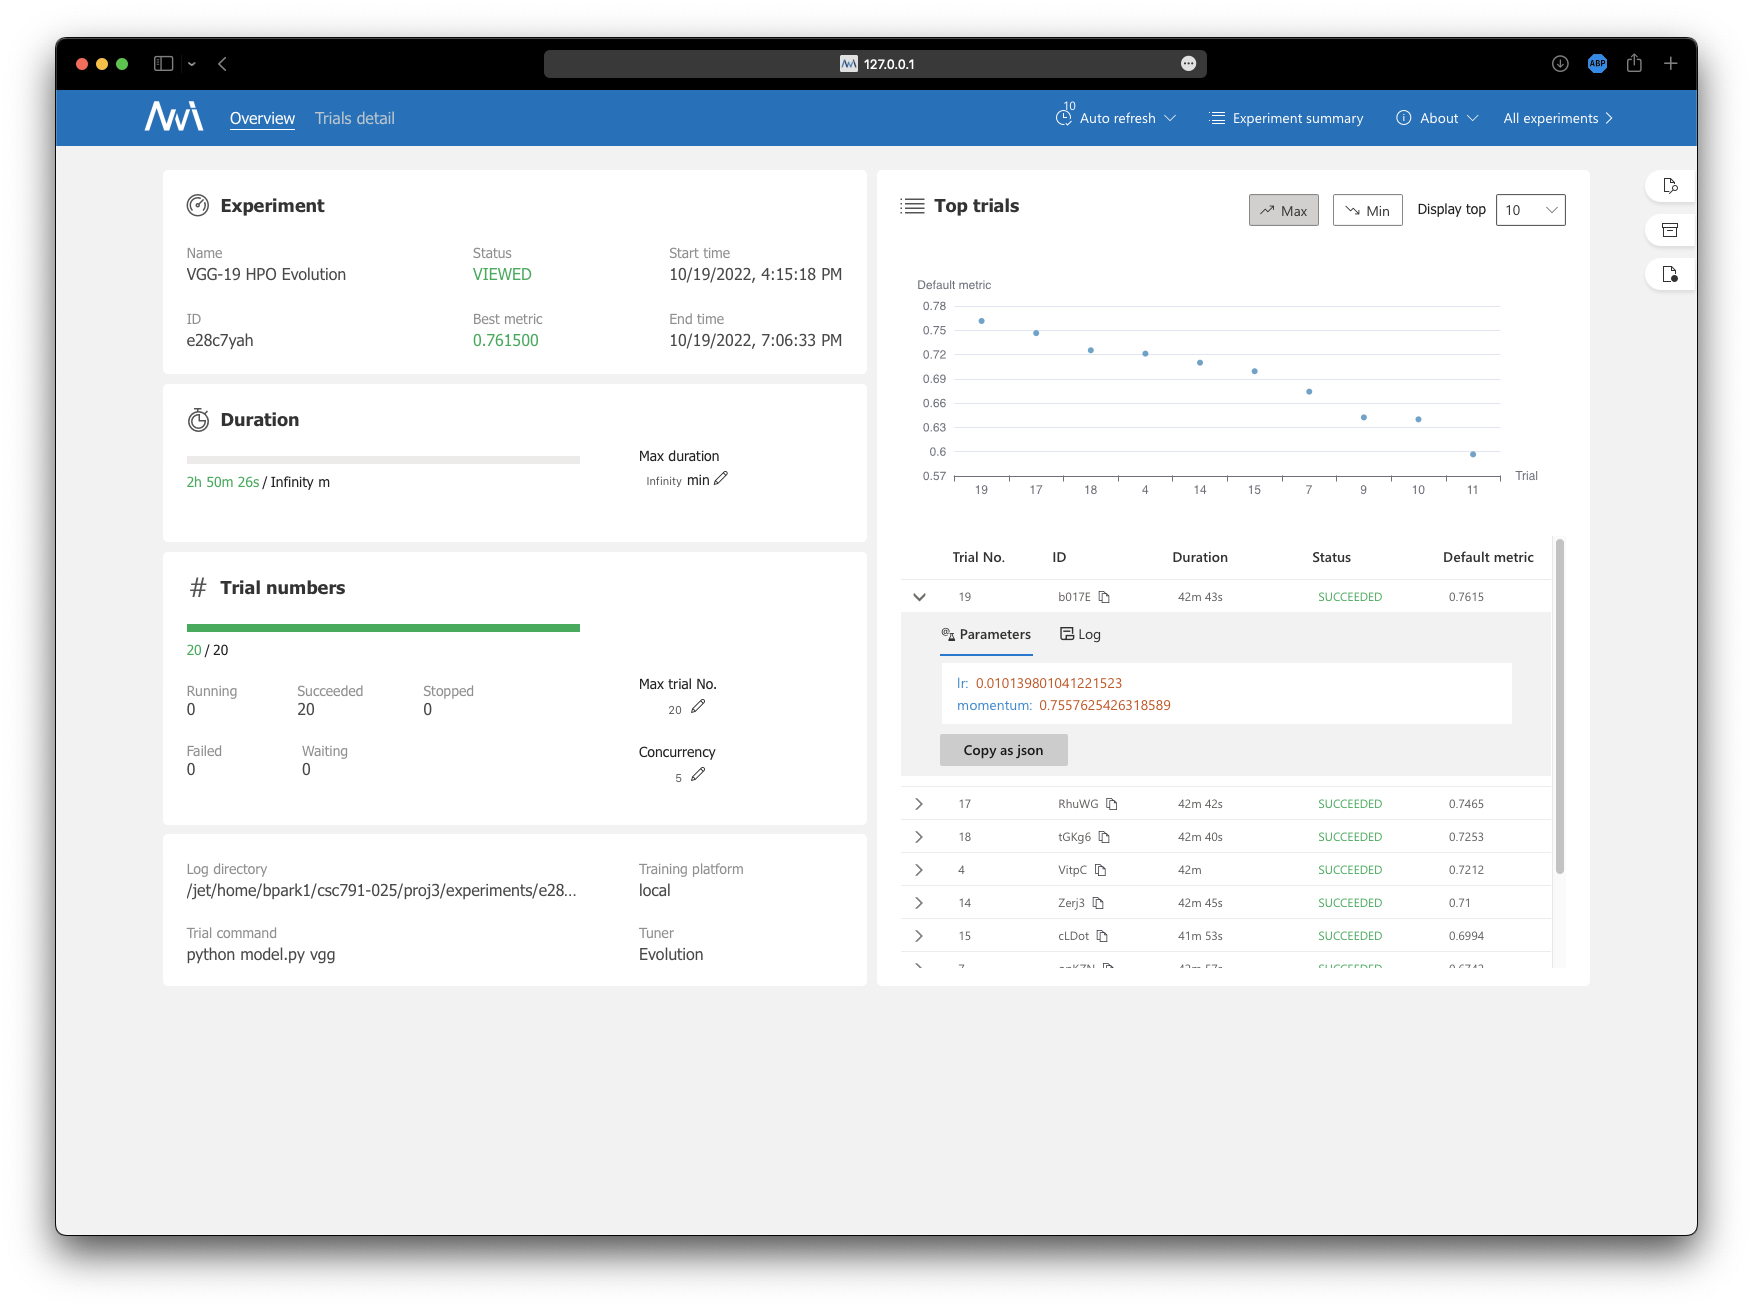
\includegraphics[width=3.5in]{../proj3/figures/vgg_evolution_overview.png}}
    \centerline{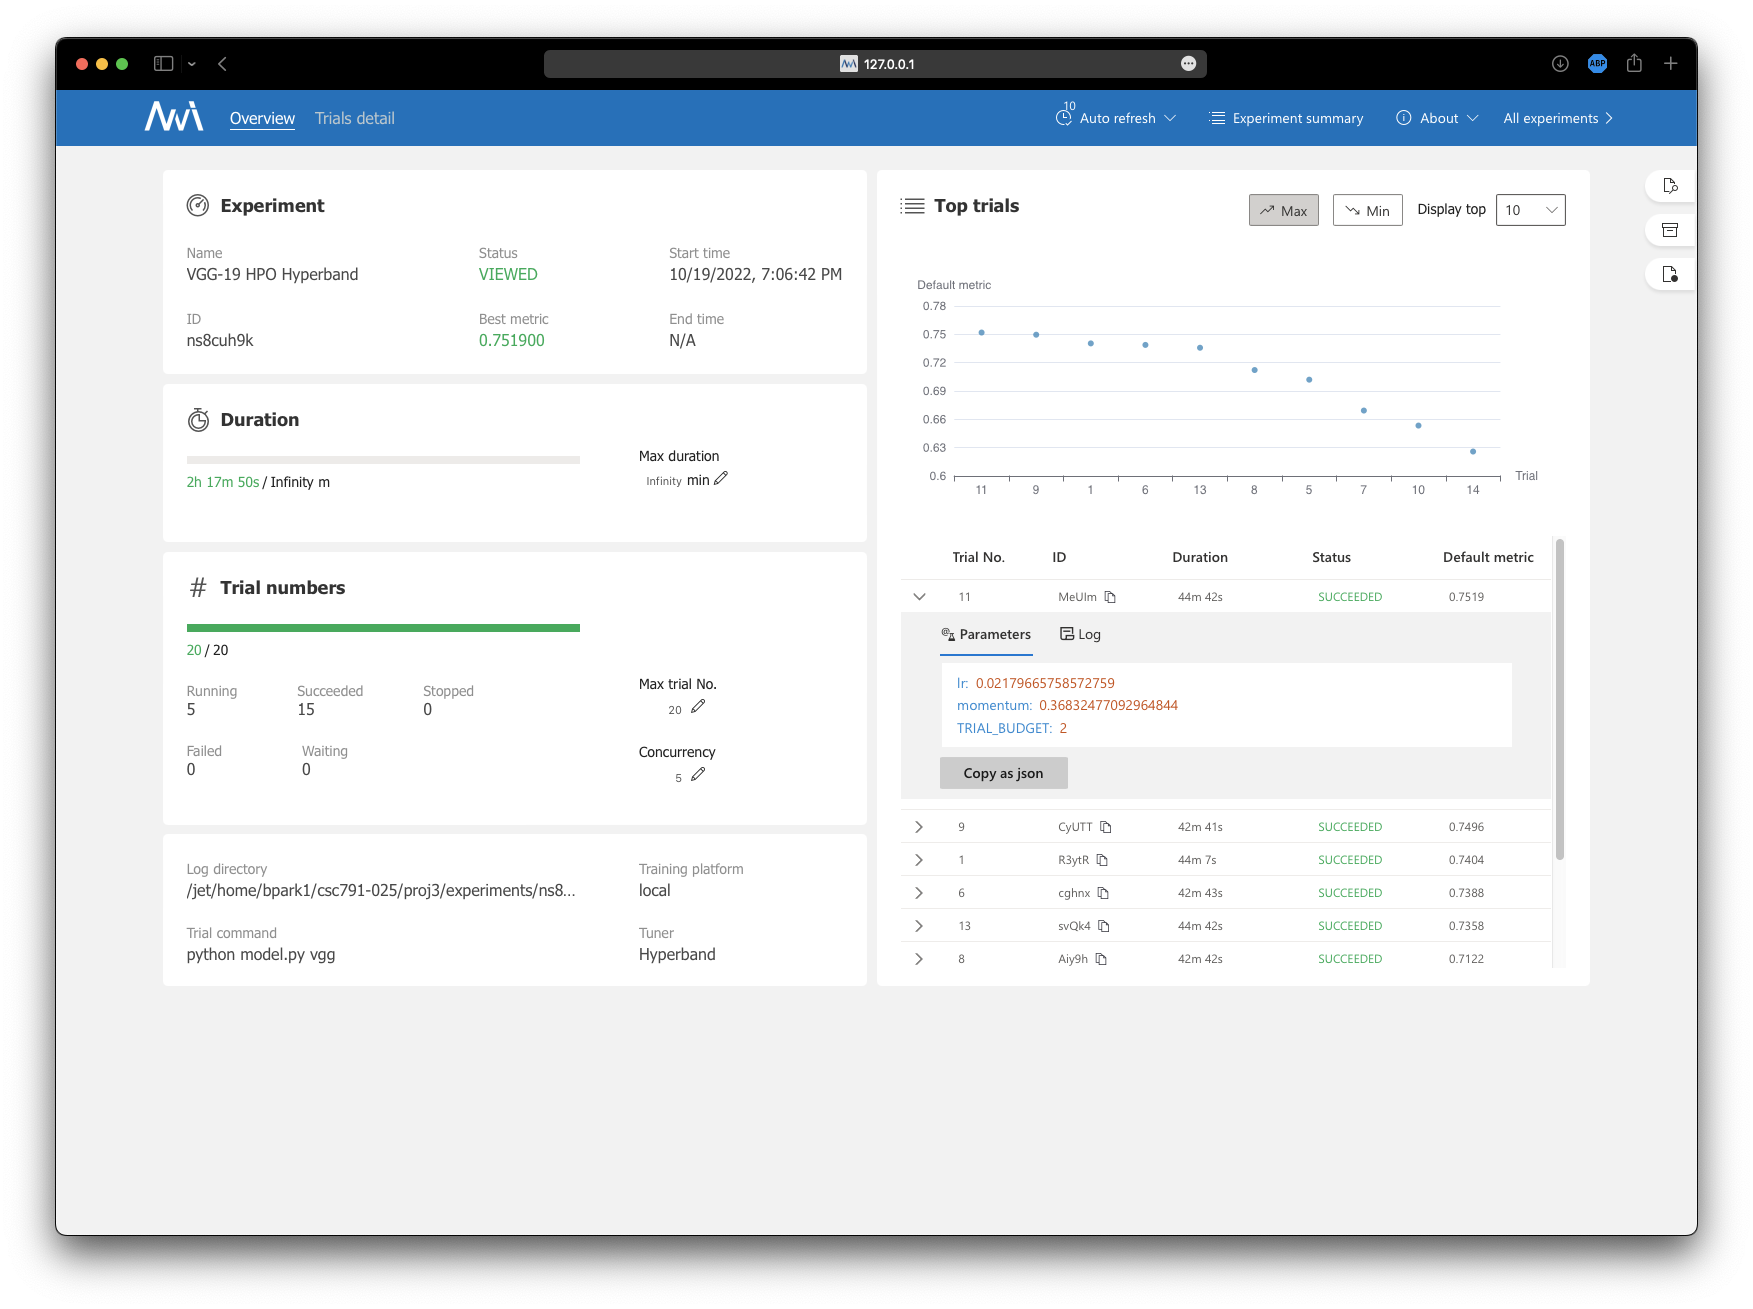
\includegraphics[width=3.5in]{../proj3/figures/vgg_hyperband_overview.png}}
    \caption{VGG HPOs on Learning Rate and Momentum}
    \label{fig:vgg-all}
\end{figure}

\end{document}
